\documentclass[thesissizeB5,twoside,onecolumn,10pt]{MechThesis}
%\documentclass[thesissizeG5]{MechThesis}
%
% Default options:
% [thesissizeG5,twoside,onecolumn,10pt,reqno,tbtags,globalpagenum,final]
%
%
% Available options:
% - size: [a4paper, letterpaper, thesissisze, thesissizeA4, thesissizeG5]
% - printing: [twoside, oneside]
% - columns: [onecolumn, twocolumns]
% - font size: [8pt, 9pt, 10pt, 11pt, 12pt]
% - position of equation numbers: [leqno, reqno]
% - split-equations numbers: [tbtags, centertags]
% - page numbers in papers: [globalpagenum, paperpagenum]
% - editing: [final, draft, printA4, cropmarks]
% - papers cover: [happyadvisor] (use it if you have more than 8 papers)
%
%
% Packages
%
% insert in this file any additional package
% Insert HERE any additional packages

\usepackage{graphicx} % Enhanced support for graphics

% Useful packages (not required):
%
% \usepackage{listings} % Typeset source code listings using LaTeX
% \usepackage{longtable} % Allow tables to flow over page boundaries
% \usepackage{mathrsfs} % Support for using RSFS fonts in maths
% \usepackage{psfrag} % Replace strings in encapsulated PostScript figures
% \usepackage{rotating} % Rotation tools, including rotated full-page floats
% \usepackage{showframe} % Draw a page-layout diagram
\usepackage[normalem]{ulem} % Package for underlining
\usepackage{mylines}
\usepackage{myplots}
\usepackage{tikz}
\usepackage{soul}
\usepackage{printlen}
\usepackage{framed}
\usepackage{nomencl}
\usepackage{multicol}
\usepackage{multirow}
\usepackage{color}

\usepackage{epstopdf, epsfig}
\usepackage{booktabs}
\usepackage{array}
\usepackage{calc}
\usepackage{microtype}
\usepackage{lscape}
\usepackage{esint,upgreek}
\usepackage{amsmath,amsfonts}
% for algorithm:
\usepackage{algorithm2e}
\RestyleAlgo{ruled}
% \usepackage{times}
% \usepackage{blindtext}

%%%%%%%%%%%%%%%%%%%%%%%%%%%%%%%%%%%%%%%%%%%%%
\usepackage[normalem]{ulem}
\usepackage{color}
\usepackage{mylines}
\usepackage{myplots}

\usepackage{lipsum}
\usepackage{cuted}
\usepackage{bm}
\usepackage{esint,upgreek,stackengine}
\usepackage[makeroom]{cancel}
\usepackage[T1]{fontenc}
\usepackage{lmodern}
\usepackage{pdfpages}
\usepackage{wrapfig}
\stackMath

%===============================================================================
%                        DO NOT TOUCH WHAT FOLLOWS
%===============================================================================
%
% The following packages are required by the MechThesis class
%
\usepackage[utf8]{inputenc} % Accept different input encodings
\usepackage[swedish,english]{babel} % Multilingual support for Plain TeX or LaTeX
\usepackage{microtype} % Subliminal refinements towards typographical perfection
\usepackage{natbib} % Flexible bibliography support
\usepackage[hidelinks]{hyperref} % Extensive support for hypertext in LaTeX
\usepackage{caption} % Correct figures and tables caption width
\usepackage{etoolbox} % Make robust some counters that are made fragile by `calc`
\robustify\setcounter
\robustify\addtocounter
\robustify\setlength
\robustify\addtolength
%
% The following packages are loaded by MechThesis.cls and need not to be loaded
% in this file:
% - color
% - amsmath
% - amsfonts
% - amssymb
% - amsthm
% - amsgen
% - crop        (if [printA4] or [cropmarks] options are used)
% - fp          (if [happyadvisor] option is used)

%===============================================================================
%                        USER-DEFINED COMMANDS
%===============================================================================
%
%% Plots style
\newcommand{\lsy}[3]{\mbox{(\kern-.4em\lineSymbolRGB[#3]{#1}{.8pt}{#2}{4pt}\kern-.4em)}}
\newcommand{\sy}[2]{\mbox{(\kern-.25em\SymbolRGB[solid]{#1}{.8pt}{#2}{4pt}\kern-.25em)}}
\newcommand{\lcap}[2]{~\,{\kern-1em\protect\mylcap{#1}{#2}}}

%% Color definition
\newcommand{\lincW}[1]{\textcolor{#1}{\rule[3pt]{.4cm}{2pt}}}
\newcommand{\lsq}[1]{{\protect\lincW{#1}}}
\definecolor{blue}{rgb}{0,0,1}
\definecolor{red}{rgb}{1,0,0}
\definecolor{black}{rgb}{0,0,0}
\definecolor{grey}{rgb}{0.5,0.5,0.5}
\definecolor{green}{rgb}{0.0,0.5,0.0}


\definecolor{fd01}{rgb}{0,0,0}
\definecolor{fd04}{rgb}{0.0862,0.3686,0.5172}
\definecolor{fd08}{rgb}{0.0000,0.6980,0.4235}
\definecolor{fd16}{rgb}{1.0000,0.8941,0.0000}
\definecolor{conv}{rgb}{1.0000,0.9098,0.7215}
\definecolor{pool}{rgb}{0.8078,0.3607,0.1372}
\definecolor{prel}{rgb}{0.6627,0.7098,0.3137}
\definecolor{batc}{rgb}{0.4549,0.4470,0.8784}
\definecolor{relu}{rgb}{0.7764,0.8274,0.3058}
\definecolor{subp}{rgb}{0.9294,0.8117,0.8156}
\definecolor{leak}{rgb}{0.2941,0.5921,0.5960}
\definecolor{full}{rgb}{0.7450,0.9882,0.7294}

\definecolor{FCN-POD}{rgb}{0.227,0.454,0.674}
\definecolor{fcn}{rgb}{0.925,0.513,0.207}
\definecolor{epod}{rgb}{0.313,0.607,0.239}

%% Review commands
\newcommand{\hlrev}[1]{{\color{magenta}\textbf{#1}}} % new added texts
\newcommand{\hlrevdd}[2]{\revd{#1} \hlrev{#2}}

\usepackage[percent]{overpic}
\usepackage{amsmath}

% For captions
\DeclareRobustCommand\full  {\tikz[baseline=-0.6ex]\draw[thick] (0,0)--(0.5,0);}
\DeclareRobustCommand\dashed{\tikz[baseline=-0.6ex]\draw[thick,dashed] (0,0)--(0.54,0);}

%
% Commands
%
% insert in this file any additional command
% Insert HERE any additional commands


% as examples here are some commands from the JFM template:
%
\newcommand\etal{\mbox{\textit{et al.}}}
\newcommand\etc{etc.\ }
\newcommand\eg{e.g.\ }

\providecommand\bnabla{\boldsymbol{\nabla}}
\providecommand\bcdot{\boldsymbol{\cdot}}

\newcommand\nRe{\mbox{$\mathrm{Re}$}}  % Reynolds number
\newcommand\nPr{\mbox{$\mathrm{Pr}$}} % Prandtl number, cf TeX's \Pr product
\newcommand\nPe{\mbox{$\mathrm{Pe}$}}  % Peclet number
\newcommand\nSt{\mbox{$\mathrm{St}$}}  % Stanton or strouhal
\newcommand\nNu{\mbox{$\mathrm{Nu}$}}  % Nusselt
\newcommand\nBi{\mbox{$\mathrm{Bi}$}}  % Biot
\newcommand\nFo{\mbox{$\mathrm{Fo}$}}  % Biot


\newcounter{boxlblcounter}  
\newcommand{\makeboxlabel}[1]{\fbox{#1}\hfill}% \hfill fills the label box
\newenvironment{boxlabel}
  {\begin{list}
    {\arabic{boxlblcounter}}
    {\usecounter{boxlblcounter}
     \setlength{\labelwidth}{3em}
     \setlength{\labelsep}{0em}
     \setlength{\itemsep}{2pt}
     \setlength{\leftmargin}{1.5cm}
     \setlength{\rightmargin}{2cm}
     \setlength{\itemindent}{0em} 
     \let\makelabel=\makeboxlabel
    }
  }
{\end{list}}


%-------------------------------------------------------------------------------
% Thesis information
%-------------------------------------------------------------------------------
%
\title[Convective heat transfer control in turbulent boundary layers]% Title used in the abstract (optional)
{% Title of the thesis
	Convective heat transfer control in turbulent boundary layers
}%

\author{Rodrigo Castellanos Garc\'ia de Blas}% Author

\affiliation
{%	Author's affiliation
	%Bioengineering and 
	Aerospace Engineering Department, Universidad Carlos III de Madrid\\
	Avenida de la Universidad, 30, Legan\'es, Spain
}%

\titel
{% Spanish title for Resumen
	Control de transferencia de calor convectivo en capa l\'imite turbulenta
}%

\anslutning
{% Author's swedish affiliation (for swedish abstract)
	Departamento de Ingenier\'ia Aeroespacial, Universidad Carlos III de Madrid\\
	Avenida de la Universidad, 30, Legan\'es, España
}%

\date{Legan\'es}{October}{2022}% City, Month, Year

\info{% Defence information (in spanish)
	Esta tesis se distribuye bajo licencia “Creative Commons \textbf{Reconocimiento – No Comercial – Sin Obra Derivada}”.\\[\baselineskip]
	%
	
\includegraphics{figures/creativecommons.pdf}
	\\[\baselineskip]% Cover info (comment if no cover image is used)
	%
	{\it Cover:} Picture by Pascal Meier in Unsplash.
	%
}


%===============================================================================
%===============================================================================
%                            BEGIN DOCUMENT
%===============================================================================
%===============================================================================

% \includeonly{overview}

\begin{document}
%===============================================================================
% Frontmatter
%===============================================================================
%
%\includepdf[pages=-]{frontpage/portada_v2_B5_front.pdf}

\frontmatter

%-------------------------------------------------------------------------------
% Cover page
%-------------------------------------------------------------------------------
%
\makecoverpage

%-------------------------------------------------------------------------------
% Dedication (comment if none)
%-------------------------------------------------------------------------------
%
\dedication{
\vspace{3cm}
\flushright{\textit{A mis padres y hermana, gracias por ser y dejarme ser...}}
\vspace{9cm}
\flushright{
	\textit{Probably it has no sense to talk about the cause of anything.\\
	You cannot talk about the cause of a chicken. [...] \\
	You cannot talk about the cause of turbulence. \\
	The cause of turbulence is probably the Big Bang. \\
	The cause of the chicken is probably also the Big Bang}\\
\vspace{1cm}
\flushright Javier Jiménez Sendín}}% \\
%\begin{minipage}[c]{0.45\linewidth}
%\begin{scriptsize}
%	"Monte-Carlo Science", \textit{Seminar Series on Aerospace Science and Technology}, Universidad Carlos III de Madrid [20$^{\text{th}}$ May, 2021]
%\end{scriptsize}
%\end{minipage} }}%


% ===============================================================================
% Acknowledgments
% ===============================================================================
\begin{acknowledgements}
%
% \begin{small}
The work enclosed in this thesis has been partially supported by the Universidad Carlos III de Madrid through a PIPF
scholarship awarded on a competitive basis, and by the following research projects: ARTURO (Active contRol of Turbulence for sUstainable aiRcraft propulsiOn), ref. PID2019-109717RB-I00/AEI/10.13039/501100011033, funded by the Spanish State Research Agency (SRA); the 2020 Leonardo Grant for Researchers and Cultural Creators AEROMATIC (Active flow control of aerodynamic flows with machine learning), funded by the BBVA Foundation with grant number IN[20]\_ING\_ING\_0163; and GloWing Starting Grant, funded by the European Research Council (ERC), under grant agreement ERC-2018.StG-803082.\\

You are reading the feelings of a 27-year-old boy after four exhausting years of work, learning, pain, passion, desperation, self-development, anxiety, ambition, disillusionment, and, above all fun. It is due to these ups rather than to the downs that I want to express my gratitude to everyone supporting me during this long and ardours adventure. It is then a must to start with my advisors. Stefano, and Andrea, if I am right now writing these lines is because of you two. Stefano, you are the closest to an \textit{academic father} to me, you are my true mentor and reference to follow. I appreciate your support, not only in my academic work but in my daily life in general. Thanks for your patience, your unstoppable effort to make me improve and your willingness to listen to me anytime. Andrea, you are one of the most special human beings that I have ever met, in all possible senses of the word special. You have the capability of driving me crazy while teaching me at the same time. You are a tireless source of ideas, problems, fun and knowledge at the same time. Thanks for being like you are and, please, keep being so for the rest of your life. You may not realise, but you two are creating a \textit{school} with a bunch of henchmen after you. Talking about henchmen and goons, it is the turn of my friend and advisor in the shadows, Marco. You are the toughest but the most willing guy I know in this world. This rare but effective combination is why I want to thank you because you have been a real pillar and stable point during my doctorate path. Thanks for helping and teaching me in the lab, and thanks for letting me help you. If my experiments did not crash, it was because Marco fixed them while shouting and cursing.

Let me travel now to the Netherlands, to Delft in particular. This is what I did almost 4 years ago, without any idea about what I was going to do there but hoping to learn something to make the trip worthwhile. There I met Marios and his gang of PhD students who welcomed me as one of them for almost 6 months. Marios, thank you very much for your effort, patience and knowledge. You convinced me of staying on the dark side of academia when I was still unsure of myself. I am also tremendously thankful to Theo. I will always repeat in my mind \textit{lunchemos} and \textit{cafemos}. You are one of my closest friends, you are really \textit{samsing}. Thanks to Beto, Kaisheng, Hongxin and Gulia for making my stay in the lab a very pleasant time.

I would like to thank you, Bernd and Guy, for being so proactive and willing to help. You taught me and introduced me to the amazing world of machine learning control and you trusted me. Thank you for your support and the rich discussion. I really hope to keep working together in the future.

Estoy especialmente agradecido a mi gran amigo Carlos. Tú me acogiste y me enseñaste cuando era un traidor, y me has seguido enseñando y apoyando desde entonces, especialmente en los últimos meses de doctorado. Gracias por contar conmigo y por hacer planes a futuro en los que quieres que esté. Además, no me puedo olvidar de Gonzalo, con quien formarnos el equipo de las \textit{cibercerves}. Carlos, Gonzalo, no sabéis cuánto bien me hicisteis en uno de los peores momentos por los que he pasado. Una simple llamada me sacaba del pozo en el que estaba.

Es turno ahora de los currelas que me han sacado las castañas del fuego. Gracias a Gianfranco por ser `el ingeniero' que puso en marcha mi tesis. Gian, amigo, eres un tipo enorme, muy valioso en lo personal y lo profesional, gracias. A los Minions, Juancho e Issac. Chavales, vosotros sí que sois de lo que no hay. Gracias por no decir que \textit{no} a nada de lo que os propongo, por animarme cuando estaba rozando el suelo y por mantenerme espabilado cuando las cosas iban bien. Espero seguir disfrutando de vuestra compañía, ya sea en el trabajo o en el Abanades con un panini los jueves. Otro especial gracias a Miguel (y por extensión a su hermano). No me conocías de nada y me brindaste toda tu ayuda desde el primer momento. Simplemente gracias por estar dispuesto, por ser el técnico al otro lado del teléfono cuando te necesitábamos y gracias, sobre todo, por ser mi amigo.

Gracias a mis compañeros de despacho en la universidad. El \textit{triángulo de las bermudas} perdurará, gracias Juanma y Manu por ser mis mejores compañeros y amigos. Gracias a Caye, por alegrarnos las estancias en el despacho con tus cánticos espontáneos. Gracias a todos los compañeros de cervezas, Luca, Sensei Cini, Besu Griego, Iván (el Rubio). Pepa pig os agradece todos los grandes momentos.

Gracias a mi amiga María. Aunque nunca lograré enseñarte matemáticas, estoy orgulloso de lo que haces, de quien eres y te estoy muy agradecido por mantenerme vivo estos años. Gracias a mi amigo de vida, Varito. Aunque nos distanciemos, es increíble ver como seguimos teniendo siempre un rato para charlar desde los tres años.

Gracias a mis compañeros en el INTA. Gracias Alex y Javi por estar siempre dispuestos a echar una mano, por comprenderme y por animarme. En especial, gracias a Jaime, te has convertido en un gran amigo en pocos meses y me has hecho quererme un poco más. Jaime, eres un tío muy grande y vas a llegar muy lejos, espero que te acuerdes de mi cuando estés sentado a la mesa con Bezos y compañía. También quiero agradecer a Esther por su comprensión y por darme la oportunidad de trabajar con ella, formando un gran equipo y aprendiendo mucho en un campo nuevo para mi hasta ahora.

Gracias a Irene por haberme impulsado desde los 18 años. Ire, tú me has enseñado a ser como soy y tú me has motivado a estar donde estoy. Gracias por haber compartido conmigo 7 preciosos años, y gracias por seguir siendo mi gran amiga.

Es imposible nombrar a todas aquellas personas que me han apoyado y animado estos últimos años. Os pido disculpas si no os veis reflejados en estas líneas, pero sabed que estoy tremendamente agradecido.

Gracias a mi familia. A mis primos y tíos, en especial a mi tío Javi, el \textit{manager}, y a mi primo Giovanni. Gracias Giova por comprenderme y por escucharme, por animarme a hacer planes chulos y por esas cervecitas tan ricas a las que me vas a invitar por ser tu primo favorito. Gracias a mis abuelos. A Felipe, el yayo, a quien le habría encantado estar hoy aquí para verme siendo doctor. A mi yaya y a mi abuela, las mujeres más fuertes que he conocido. Y a mi abuelo, por estar siempre cerca, cuidándome y queriéndome por encima de todo.

A mi hermana. Pauli, a pesar de nuestros más y nuestros menos, debes saber que eres muy importante para mí. Gracias por ser la peor y la mejor de las hermanas. Gracias por haberme hecho crecer. Y, sobre todo, gracias por quererme como tú lo haces.

Acabo agradeciendo a las personas más importantes en mi vida, a mis padres. Mamá, papá, mirad lo que he conseguido. Esto es por vosotros. Gracias por ser, estar y dejarme ser desde que era un niño. Vuestro apoyo no tiene medida y nunca podré expresar mi gratitud.

% \end{small}
\end{acknowledgements}



%-------------------------------------------------------------------------------
% Abstract (English)
%-------------------------------------------------------------------------------
%
\clearpage \newpage
\ \thispagestyle{empty}
\begin{abstract}
	\noindent 
	The sustainable development of our society opens up concerns in several fields of engineering, including energy management, production, and the impact of our technology, being thermal management a common issue to be addressed. The investigation reported in this manuscript focuses on understanding, controlling and optimizing the physical processes involving convective heat transfer in turbulent wall-bounded flows. The content is divided into two main blocks, namely the investigation of classic open-loop active-control techniques to control heat transfer, and the technological development of machine-learning strategies to enhance the performance of flow control in the field of convective heat transfer. 
	
    The first block focuses on actuator technology, applying dielectric-barrier discharge (DBD) plasma actuators and a pulsed slot jet in crossflow (JICF), respectively, to control the convective heat transfer in a turbulent boundary layer (TBL) over a flat plate. In the former, an array of DBD plasma actuators is employed to induce pairs of counter-rotating, streamwise-aligned vortices embedded in the TBL to reduce heat transfer downstream of the actuation. The whole three-dimensional mean flow field downstream of the plasma actuator is reconstructed from stereoscopic particle image velocimetry (PIV). Infrared thermography (IR) measurements coupled with a heated thin foil provide ensemble-averaged convective heat transfer distributions downstream of the actuators. The combination of the flow field and heat transfer measurements provides a complete picture of the fluid-dynamic interaction of plasma-induced flow with local turbulent transport effects. The plasma-induced streamwise vortices are stationary and confined across the spanwise direction due to the action of the plasma discharge. The opposing plasma discharge causes a mass- and momentum-flux deficit within the boundary layer, leading to a low-velocity region that grows in the streamwise direction and which is characterised by an increase in displacement and momentum thicknesses. This low-velocity ribbon travels downstream, promoting streak-alike patterns of reduction in the convective heat transfer distribution. Near the wall, the plasma-induced jets divert the main flow due to the DBD-actuator momentum injection and the suction on the surrounding fluid by the emerging jets. The stationarity of the plasma-induced vortices makes them persistent far downstream, reducing the convective heat transfer.
    
    Conversely, the target of the second paper in this first block is to enhance convective heat transfer rather than reduce it. A fully modulated, pulsed, slot JICF is used to perturb the TBL. The slot-jet actuator, flush-mounted and aligned in the spanwise direction, is controlled based on two design parameters, namely the duty cycle ($DC$) and the pulsation frequency ($f$). Heat transfer and flow-field measurements are performed to characterise the control performance using IR thermography and planar PIV, respectively. A parametric study on $f$ and $DC$ is carried out to assess their effect on the heat transfer distribution. The vorticity fields are reconstructed from the Proper Orthogonal Decomposition (POD) modes, retrieving phase information. The flow topology is considerably altered by the jet pulsation, even compared to the case of a steady jet. The results show that both the jet penetration in the streamwise direction and the overall Nusselt number increase with increasing $DC$. However, the frequency at which the Nusselt number is maximised is independent of the duty cycle. A wall-attached jet rises from the slot accompanied by a pair of counter-rotating vortices that promote flow entrainment and mixing. Eventually, a simplified model is proposed which decouples the effect of $f$ and $DC$ in the overall heat transfer enhancement, with a good agreement with experimental data. The cost of actuation is also quantified in terms of the amount of injected fluid during the actuation, leading to conclude that the lowest duty cycle is the most efficient for heat transfer enhancement among the tested set.
	
    The second block of the thesis splits into a comparative assessment of machine learning (ML) methods for active feedback flow control and an application of linear genetic algorithms to an experimental convective heat transfer enhancement problem. First, the comparative study is carried out numerically based on a well-established benchmark problem, the drag reduction of a two-dimensional Kármán vortex street past a circular cylinder at a low Reynolds number ($Re=100$). The flow is manipulated with two blowing/suction actuators on the upper and lower side of a cylinder. The feedback employs several velocity sensors. Two probe configurations are evaluated: 5 and 11 velocity probes located at different points around the cylinder and in the wake. The control laws are optimized with Deep Reinforcement Learning (DRL) and Linear Genetic Programming Control (LGPC). Both methods successfully stabilize the vortex alley and effectively reduce drag while using small mass flow rates for the actuation. DRL features higher robustness with respect to variable initial conditions and noise contamination of the sensor data; on the other hand, LGPC can identify compact and interpretable control laws, which only use a subset of sensors, thus allowing reducing the system complexity with reasonably good results.
    
    The gained experience and knowledge of machine-learning methods motivated the last study enclosed in this thesis, which utilises linear genetic algorithm control (LGAC) to identify the best actuation parameters in an experimental application. The actuator is a set of six slot jets in crossflow aligned with the freestream. An open-loop optimal periodic forcing is defined by the carrier frequency ($f$), the duty cycle ($DC$) and the phase between actuators ($\phi$) as control parameters. The control laws are optimised with respect to the unperturbed TBL and the steady-jet actuation. The cost function includes wall convective heat transfer and the cost of the actuation, thus leading to a multi-objective optimisation problem. Surprisingly, the LGAC algorithm converges to the same frequency and duty cycle for all the actuators. This frequency is equivalent to the optimal frequency reported in the second study of the first block of this thesis. The performance of the controller is characterised by IR thermography and PIV measurements. The action of the jets considerably alters the flow topology compared to the steady-jet actuation,  yielding a slightly asymmetric flow field.  The phase difference between multiple jet actuation has shown to be very relevant and the main driver of flow asymmetry. A POD analysis concludes the shedding phenomena characterising the steady-jet actuation, while the optimised controller exhibits an elongated large-scale structure just downstream of the actuator.
    
    The investigation carried out in this thesis sheds some light on the application of different flow control strategies to the field of convective heat transfer. From the utilisation of plasma actuators and a single jet in cross flow to the development of sophisticated control logic, the results point to the exceptional potential of machine learning control in unravelling unexplored controllers within the actuation space. Ultimately, this work demonstrates the viability of employing sophisticated measurement techniques together with advanced algorithms in an experimental investigation, paving the way towards more complex applications involving feedback information.
		%
		\keywords{Convective heat transfer, flow control, machine learning, jet in cross flow, plasma actuator, turbulent boundary layer, reinforcement learning, genetic programming, genetic algorithms.}
		%
\end{abstract}


%-------------------------------------------------------------------------------
% Resumen
%-------------------------------------------------------------------------------
%
\clearpage \newpage
\ \thispagestyle{empty}
\begin{abstrakt}

	\noindent El desarrollo sostenible de nuestra sociedad abre preocupaciones en varios campos de la ingeniería, incluyendo la gestión de la energía, la producción y el impacto de nuestra tecnología, siendo la gestión térmica un tema común a tratar. La investigación que se presenta en este manuscrito se centra en la comprensión, el control y la optimización de los procesos físicos que implican la transferencia de calor por convección en flujos turbulentos de pared. El contenido se divide en dos bloques principales: la investigación de las técnicas clásicas de control activo de lazo abierto para controlar la transferencia de calor, y el desarrollo tecnológico de estrategias de aprendizaje automático para mejorar el rendimiento del control del flujo en el campo de la transferencia de calor por convección. 
    
    
    El primer bloque se centra en la tecnología de los actuadores, aplicando actuadores de plasma de descarga de barrera dieléctrica (dielectric barrier dicharge, DBD) y un chorro con forma de ranura pulsado en flujo cruzado (jet in crossflow, JICF), respectivamente, para controlar la transferencia de calor por convección en una capa límite turbulenta (turbulent boundary layer, TBL) sobre una placa plana. En el primero, se emplea un conjunto de actuadores de plasma DBD para inducir pares de vórtices contra-rotativos, alineados con la corriente e incrustados en la TBL para reducir la transferencia de calor aguas abajo de la actuación. El campo de flujo medio tridimensional completo aguas abajo del actuador de plasma se reconstruye a partir de la velocimetría de imagen de partículas estereoscópica (particle image velocimetry, PIV). Las mediciones de termografía infrarroja (IR) junto a una fina lámina calentada proporcionan distribuciones de transferencia de calor convectiva promediadas aguas abajo de los actuadores. La combinación de las mediciones del campo de flujo y de la transferencia de calor proporciona una imagen completa de la interacción fluido-dinámica del flujo inducido por el plasma con los efectos locales de transporte turbulento. Los vórtices en el sentido de la corriente inducidos por plasma son estacionarios y están confinados transversalmente debido a la acción de la descarga de plasma. La descarga de plasma en oposición causa un déficit de flujo de masa y de momento dentro de la capa límite, lo que conduce a una región de baja velocidad que crece en la dirección de la corriente y que se caracteriza por un aumento de los espesores de desplazamiento y de momento. Esta zona de baja velocidad se desplaza corriente abajo, promoviendo patrones de reducción similares a rayas en los que se reduce la transferencia de calor por convección. Cerca de la pared, los chorros inducidos por el plasma desvían el flujo principal debido a la inyección de momento del actuador DBD y a la succión sobre el fluido circundante por parte de los chorros emergentes. La estacionariedad de los vórtices inducidos por el plasma los hace persistentes aguas abajo, reduciendo la transferencia de calor por convección.
    
    Por el contrario, el objetivo del segundo trabajo de este primer bloque es mejorar la transferencia de calor por convección en lugar de reducirla. Se utiliza un JICF, pulsado y con forma de ranura, totalmente modulado para perturbar la TBL. El actuador de chorro, montado a ras y alineado en la dirección transversal, se controla en base a dos parámetros de diseño, a saber, el ciclo de trabajo ($DC$) y la frecuencia de pulsación ($f$). Se realizan mediciones de la transferencia de calor y del campo de flujo para caracterizar el rendimiento del control mediante termografía IR y PIV planar, respectivamente. Se lleva a cabo un estudio paramétrico de $f$ y $DC$ para evaluar su efecto en la distribución de la transferencia de calor. Los campos de vorticidad se reconstruyen a partir de los modos de descomposición ortogonal adecuada (POD), recuperando la información de fase. La topología del flujo se ve considerablemente alterada por la pulsación del chorro, incluso en comparación con el caso de un chorro estacionario. Los resultados muestran que tanto la penetración del chorro en la dirección de la corriente como el número Nusselt global aumentan con el incremento de $DC$. Sin embargo, la frecuencia a la que se maximiza el número Nusselt es independiente del ciclo de trabajo. Un chorro adherido a la pared sale de la ranura acompañado de un par de vórtices contrarrotantes que promueven el arrastre y la mezcla del flujo. Finalmente, se propone un modelo simplificado que desacopla el efecto de $f$ y $DC$ en la mejora global de la transferencia de calor, con un buen acuerdo con los datos experimentales. También se cuantifica el coste de la actuación en términos de la cantidad de fluido inyectado durante la actuación, llegando a la conclusión de que el ciclo de trabajo más bajo es el más eficiente para la mejora de la transferencia de calor entre el conjunto probado.

    El segundo bloque de la tesis se divide en una evaluación comparativa de los métodos de aprendizaje automático (machine learning, ML) para el control activo del flujo por retroalimentación y una aplicación de algoritmos genéticos lineales a un problema experimental de mejora de la transferencia de calor por convección. En primer lugar, el estudio comparativo se realiza numéricamente a partir de un problema de referencia bien establecido: la reducción de la resistencia aerodinámica de una calle de vórtices de Kármán bidimensional tras un cilindro circular a un número de Reynolds bajo ($Re=100$). El flujo se manipula con dos actuadores de soplado/succión en la parte superior e inferior de un cilindro. La retroalimentación emplea varios sensores de velocidad. Se evalúan dos configuraciones de sondas: 5 y 11 sondas de velocidad situadas en diferentes puntos alrededor del cilindro y en la estela. Las leyes de control se optimizan con el aprendizaje profundo por refuerzo (Deep Reinforcement Learning, DRL) y el control por programación genética lineal (Linear Genetic Programming Control, LGPC). Ambos métodos estabilizan con éxito la calle de vórtices y reducen de manera efectiva la resistencia al tiempo que usan caudales másicos pequeños para la actuación. El DRL se caracteriza por una mayor robustez con respecto a la variación de la condición inicial y a la contaminación por ruido de los datos de los sensores; por otro lado, el LGPC puede identificar leyes de control compactas e interpretables, que sólo utilizan un subconjunto de sensores, lo que permite reducir la complejidad del sistema con resultados razonablemente buenos.

    La experiencia adquirida y el conocimiento de los métodos de aprendizaje automático motivaron el último estudio incluido en esta tesis, que utiliza el control por algoritmo genético lineal (Linear Genetic Algorithm Control, LGAC) para identificar los mejores parámetros de actuación en una aplicación experimental. El actuador es un conjunto de seis chorros con forma de ranura en flujo cruzado y alineados con la corriente principal. Se define una ley de forzado periódica en lazo abierto mediante la frecuencia portadora ($f$), el ciclo de trabajo ($DC$) y la fase entre actuadores ($\phi$) como parámetros de control. Las leyes de control se optimizan con respecto a la TBL no perturbada y la actuación de chorro constante. La función de coste incluye la transferencia de calor por convección de la pared y el coste de la actuación, lo que da lugar a un problema de optimización multiobjetivo. Sorprendentemente, el algoritmo LGAC converge a la misma frecuencia y ciclo de trabajo para todos los actuadores. Esta frecuencia es equivalente a la frecuencia óptima reportada en el segundo estudio del primer bloque de esta tesis. El rendimiento del controlador se caracteriza mediante termografía IR y mediciones PIV. La acción de los chorros altera considerablemente la topología del flujo en comparación con la actuación de los chorros constantes, dando lugar a un campo de flujo ligeramente asimétrico. La diferencia de fase entre la actuación de múltiples chorros ha demostrado ser muy relevante y el principal impulsor de la asimetría del flujo. Un análisis POD concluye los fenómenos de desprendimiento de vórtices que caracterizan la actuación de chorro constante, mientras que el controlador optimizado muestra una estructura alargada a gran escala justo aguas abajo del actuador.
    
    La investigación llevada a cabo en esta tesis arroja algo de luz sobre la aplicación de diferentes estrategias de control de flujo en el campo de la transferencia de calor por convección. Desde la utilización de actuadores de plasma y un único chorro en flujo cruzado hasta el desarrollo de una sofisticada lógica de control, los resultados apuntan al excepcional potencial del control por aprendizaje automático para desentrañar controladores inexplorados dentro del espacio de actuación. En última instancia, este trabajo demuestra la viabilidad de emplear sofisticadas técnicas de medición junto con algoritmos avanzados en una investigación experimental, allanando el camino hacia aplicaciones más complejas que implican información de retroalimentación.

    %
    \palabrasclave{Transferencia de calor por convección, control de flujo, aprendizaje automático, chorro en flujo cruzado, actuador de plasma, capa límite turbulenta, aprendizaje por refuerzo, programación genética, algoritmos genéticos.}
    %
\end{abstrakt}


%-------------------------------------------------------------------------------
% Preface page
%-------------------------------------------------------------------------------
%
\clearpage \newpage
\ \thispagestyle{empty}
\begin{preface}
This dissertation deals with the control of convective heat transfer enhancement in wall-bounded flows under turbulent conditions, exploring active control techniques and the incorporation of model-free algorithms based on machine learning.
%
A brief introduction of the basic concepts and methods is presented in the first part.
%
The second part contains four scientific journal publications under the umbrella of this dissertation and an additional methodological article which is relevant for the herein presented investigation.
%
The papers are adjusted to comply with the present thesis format for consistency, but their contents have not been altered as compared with their original counterparts.
\end{preface}


%-------------------------------------------------------------------------------
% Division of work between authors
%-------------------------------------------------------------------------------
%
\begin{divisionofwork}
	The desciption of the individual author contributions is presented by means of CRediT \footnote{Brand, A., Allen, L., Altman, M., Hlava, M. and Scott, J. (2015), Beyond authorship: attribution, contribution, collaboration, and credit. Learned Publishing, 28: 151-155. https://doi.org/10.1087/20150211}. CRediT (Contributor Roles Taxonomy) provides an accurate and detailed description of the authors' diverse contributions to the published work.% A summarised description of the CRediT categories is provided in Table~\textit{CRediT}.

%-----------------------------------------------
\paperitem % Uncertainty analysis
	\textbf{RC:} Methodology, Software, Validation, Formal analysis, Investigation, Data Curation, Writing - Original Draft, Writing - Review \& Editing, Visualization;
	\textbf{AG:} Methodology, Software, Formal analysis, Investigation, Writing - Original Draft, Writing - Review \& Editing, Visualization;
	\textbf{CSV:} Conceptualization, Methodology, Software, Writing - Original Draft, Writing - Review \& Editing, Supervision;
	\textbf{SD:} Conceptualization, Methodology, Software, Resources, Writing - Original Draft, Writing - Review \& Editing, Supervision, Project administration, Funding acquisition.

%-----------------------------------------------
\paperitem % Plasmas
	\textbf{RC:} Conceptualization, Methodology, Software, Validation, Formal analysis, Investigation, Data Curation, Writing - Original Draft, Writing - Review \& Editing, Visualization;
	\textbf{TM:} Conceptualization, Methodology, Software, Validation, Formal analysis, Investigation, Data Curation, Writing - Original Draft, Writing - Review \& Editing, Visualization;
	\textbf{SD:} Conceptualization, Methodology, Writing - Review \& Editing, Supervision, Project administration, Funding acquisition;
	\textbf{AI:} Conceptualization, Methodology, Writing - Review \& Editing, Supervision, Project administration, Funding acquisition;
	\textbf{MK:} Conceptualization, Methodology, Software, Resources, Writing - Review \& Editing, Visualization, Supervision, Project administration, Funding acquisition;

%-----------------------------------------------
\paperitem % Slot jet in crossflow
	\textbf{RC:} Methodology, Software, Validation, Formal analysis, Investigation, Data Curation, Writing - Original Draft, Writing - Review \& Editing, Visualization, Project administration;
	\textbf{GS:} Software, Validation, Investigation, Writing - Original Draft, Writing - Review \& Editing, Visualization;
	\textbf{MR:} Methodology, Validation, Investigation, Writing - Review \& Editing, Supervision;
	\textbf{AI:} Conceptualization, Methodology, Investigation, Resources, Writing - Review \& Editing, Supervision, Project administration, Funding acquisition;
	\textbf{SD:} Conceptualization, Methodology, Validation, Resources, Writing - Review \& Editing, Supervision, Project administration, Funding acquisition.

%-----------------------------------------------
\paperitem % LGPC vs RL
	\textbf{RC:} Conceptualization, Methodology, Software, Validation, Formal analysis, Investigation, Data Curation, Writing - Original Draft, Writing - Review \& Editing, Visualization, Project administration;
	\textbf{GCM:} Software, Formal analysis, Writing - Original Draft, Writing - Review \& Editing, Visualization;
	\textbf{IF:} Methodology, Software, Writing - Original Draft, Writing - Review \& Editing, Visualization;
	\textbf{BN:} Conceptualization, Resources, Writing - Review \& Editing, Supervision, Funding acquisition;
	\textbf{AI:} Conceptualization, Resources, Writing - Review \& Editing, Supervision, Project administration, Funding acquisition;
	\textbf{SD:} Conceptualization, Resources, Writing - Original Draft, Writing - Review \& Editing, Supervision, Project administration, Funding acquisition;
		
\paperitem % LGAC in TBL for HTE
	\textbf{RC:} Conceptualization, Methodology, Software, Validation, Formal analysis, Investigation, Data Curation, Writing - Original Draft, Writing - Review \& Editing,
Visualization, Project administration ;
	\textbf{AI:} Conceptualization, Methodology, Resources, Writing - Review \&
Editing, Supervision, Project administration, Funding acquisition;
	\textbf{SD:} Conceptualization, Methodology, Software, Validation, Investigation, Resources, Writing - Review \& Editing, Supervision, Project administration, Funding acquisition.\\%

\vspace{1cm}
\noindent Acronyms correspond to:
\begin{itemize}
    \item[RC] Rodrigo \textbf{Castellanos}. Universidad Carlos III de Madrid. \small{\textit{PhD Candidate}}.
    \item[SD] Stefano \textbf{Discetti}. Universidad Carlos III de Madrid. \small{\textit{Advisor and Tutor}}. 
    \item[AI] Andrea \textbf{Ianiro}. Universidad Carlos III de Madrid. \small{\textit{Advisor}}.
    \item[MR] Marco \textbf{Raiola}. Universidad Carlos III de Madrid.
    \item[CSV] Carlos \textbf{Sanmiguel-Vila}. Universidad Carlos III de Madrid.
    \item[AG] Alejandro \textbf{G\"uemes}. Universidad Carlos III de Madrid.
    \item[GS] Gianfranco \textbf{Salih}. Universidad Carlos III de Madrid.
    \item[IF] Ignacio \textbf{de la Fuente}. Universidad Carlos III de Madrid.
    \item[MK] Marios \textbf{Kotsonis}. Technische Universiteit Delft.
    \item[TM] Theodoros \textbf{Michelis}. Technische Universiteit Delft.
    \item[BN] Bernd R. \textbf{Noack}. Harbin Institute of Technology.
    \item[GCM] Guy Y. \textbf{Cornejo Maceda}. Harbin Institute of Technology.
\end{itemize}


%\begin{table}
%\centering
%\begin{tabular}{>{\raggedright\arraybackslash}p{0.25\linewidth-2\tabcolsep}
%>{\raggedright\arraybackslash}p{0.75\linewidth-2\tabcolsep}}
%\toprule
%\tiny{Term} & \tiny{Definition } \\
%\midrule
%\tiny{Conceptualization} & \tiny{Ideas; formulation or evolution of overarching research goals and aims } \\
%\tiny{Methodology} & \tiny{Development or design of methodology; creation of models} \\
%\tiny{Software} & \tiny{Programming, software development; designing computer programs; implementation of the computer code and supporting algorithms; testing of existing code components} \\
%\tiny{Validation} & \tiny{Verification, whether as a part of the activity or separate, of the overall replication/ reproducibility of results/experiments and other research outputs} \\
%\tiny{Formal analysis} & \tiny{Application of statistical, mathematical, computational, or other formal techniques to analyze or synthesize study data} \\
%\tiny{Investigation} & \tiny{Conducting a research and investigation process, specifically performing the experiments, or data/evidence collection} \\
%\tiny{Resources} & \tiny{Provision of study materials, reagents, materials, patients, laboratory samples, animals, instrumentation, computing resources, or other analysis tools} \\
%\tiny{Data Curation} & \tiny{Management activities to annotate (produce metadata), scrub data and maintain research data (including software code, where it is necessary for interpreting the data itself) for initial use and later reuse} \\
%\tiny{Writing - Original Draft} & \tiny{Preparation, creation and/or presentation of the published work, specifically writing the initial draft (including substantive translation)} \\
%\tiny{Writing - Review \& Editing} & \tiny{Preparation, creation and/or presentation of the published work by those from the original research group, specifically critical review, commentary or revision – including pre-or postpublication stages} \\
%\tiny{Visualization} & \tiny{Preparation, creation and/or presentation of the published work, specifically visualization/ data presentation} \\
%\tiny{Supervision} & \tiny{Oversight and leadership responsibility for the research activity planning and execution, including mentorship external to the core team} \\
%\tiny{Project administration} & \tiny{Management and coordination responsibility for the research activity planning and execution} \\
%\tiny{Funding acquisition} & \tiny{Acquisition of the financial support for the project leading to this publication} \\
%\bottomrule
%\end{tabular}
%\caption*{CRediT: Description of CRediT categories based on Brand et al. (2015), Learned Publishing 28(2).}
%\end{table}
\end{divisionofwork}

%-------------------------------------------------------------------------------
% Additional publications (comment if none)
%-------------------------------------------------------------------------------
%
\clearpage \newpage
\ \thispagestyle{empty}
\clearpage
\begin{otherpublications}
	The following papers, although related to the field of aerospace engineering, are not included in this thesis.\\

  \paperitem%
    {Bombardieri, R., Cavallaro, R., Castellanos, R. \& Auricchio, F.}% Authors
    {2021}% Year
    {On the dynamic fluid–structure stability response of an innovative airplane configuration}% Title
    {J. Fluids Struct.}% Journal
    {105}% Volume
    {}% Number
    {103347}% Pages

\vspace{0.3cm}

	\paperitem%
		{Mantec{\'o}n, R., Rufo-Mart{\'i}n, C., Castellanos, R. \& Diaz-Alvarez, J.}% Authors
		{2022}% Year
		{Experimental assessment of thermal gradients and layout effects on the mechanical performance of components manufactured by fused deposition modeling}% Title
		{Rapid Prototyp. J.}% Journal
		{28}% Volume
		{8}% Number
		{1598-1608}% Page
\end{otherpublications}

%-------------------------------------------------------------------------------
% Conferences (comment if none)
%-------------------------------------------------------------------------------
\begin{conferences}
	Part of the work in this thesis has been presented at the following international conferences. The presenting author is underlined.

%----------------------------------------
  \conferenceitem%
    {Bombardieri, R., \underline{Cavallaro, R.}, Castellanos, R. \& Auricchio, F.}% Authors
    {2019}% Year
    {Studies on Lateral-directional Coupled Flight Dynamics and Aeroelasticity of a PrandtlPlane}% Title
    {AIAA Scitech 2019 Forum}% Conference
    {San Diego, USA}% Location

%----------------------------------------
  \conferenceitem%
    {\underline{Castellanos, R.}, Michelis, T., Discetti, S., Ianiro, A. \& Kotsonis, M.}% Authors
    {2020}% Year
    {Turbulent convective heat transfer control with plasma actuators}% Title
    {73rd Annual Meeting of the APS Division of Fluid Dynamics}% Conference
    {Chicago, USA (online)}% Location

%----------------------------------------
  \conferenceitem%
    {\underline{Castellanos, R.}, Michelis, T., Discetti, S., Ianiro, A. \& Kotsonis, M.}% Authors
    {2021}% Year
    {Active Control of Turbulent Convective Heat Transfer with Plasma Actuators}% Title
    {iTi Conference in Turbulence}% Conference
    {Bertinoro, Italy (online)}% Location

%----------------------------------------
	\conferenceitem%
		{\underline{Foroozan, F.}, Güemes, A., Castellanos, R., Raiola, M., Ianiro, A., \& Discetti, S.}% Authors
		{2021}% Year
		{Correlation between wall and flow fields in turbulent boundary layer: a synchronized measurement}% Title
		{19th International Symposium on Flow Visualization}% Conference
		{Shanghai, China (online)}% Location

%----------------------------------------
	\conferenceitem%
		{\underline{Castellanos, R.}, Michelis, T., Discetti, S., Ianiro, A. \& Kotsonis, M.}% Authors
		{2021}% Year
		{Streamwise-plasma-actuator vortex generators for heat transfer control}% Title
		{19th International Symposium on Flow Visualization}% Conference
		{Shanghai, China (online)}% Location

%----------------------------------------
	\conferenceitem%
		{\underline{Salih, G.}, Castellanos, R., Raiola, M., Ianiro, A., \& Discetti, S.}% Authors
		{2021}% Year
		{Active flow control of turbulent boundary layer with a crossflow slot jet}% Title
		{19th International Symposium on Flow Visualization}% Conference
		{Shanghai, China (online)}% Location

%----------------------------------------
	\conferenceitem%
		{\underline{Castellanos, R.}, Salih, G., Raiola, M., Ianiro, A., \& Discetti, S.}% Authors
		{2021}% Year
		{Pulsed slot jets in crossflow for heat transfer enhancement}% Title
    {13th International ERCOFTAC Symposium on Engineering, Turbulence, Modeling and Measurements}% Conference
    {Rhodes, Greece}% Location

%----------------------------------------
	\conferenceitem%
		{\underline{Castellanos, R.}, de la Fuente, I. Cornejo-Maceda, G. Y., Noack, R. R., Ianiro, A., \& Discetti, S.}% Authors
		{2021}% Year
		{Machine Learning flow control in the few sensors limit}% Title
    {74rd Annual Meeting of the APS Division of Fluid Dynamics}% Conference
    {Phoenix, USA}% Location

%----------------------------------------
	\conferenceitem%
		{\underline{Castellanos, R.}, Salih, G., Raiola, M., Ianiro, A., \& Discetti, S.}% Authors
		{2022}% Year
		{Pulsed jets in cross-flow for convective heat transfer enhancement}% Title
    {1st Spanish Fluid Mechanics Conference}% Conference
    {C\'{a}diz, Spain}% Location

%----------------------------------------
	\conferenceitem%
		{\underline{Foroozan, F.}, Güemes, A., Castellanos, R., Raiola, M., Ianiro, A., \& Discetti, S.}% Authors
		{2022}% Year
		{Synchronized measurements of wall and flow fields in a turbulent boundary layer}% Title
    {1st Spanish Fluid Mechanics Conference}% Conference
    {C\'{a}diz, Spain}% Location

%----------------------------------------
	\conferenceitem%
		{\underline{Bowen-Varela, J.}, Castellanos, R., Farzamnik, E., Gorgues, A., Ianiro, A., \& Andr\'{e}, E.}% Authors
		{2022}% Year
		{Nonlinear interpolation of steady transonic flows via manifold learning and neural
networks}% Title
    {1st Spanish Fluid Mechanics Conference}% Conference
    {C\'{a}diz, Spain}% Location

%----------------------------------------
	\conferenceitem%
		{Güemes, A., Mart\'{i}n, A. Castellanos, R., Flores, O. \& \underline{Discetti, S.}}% Authors
		{2022}% Year
		{Active drag reduction in minimal flow units via deep reinforcement learning}% Title
    {1st Spanish Fluid Mechanics Conference}% Conference
    {C\'{a}diz, Spain}% Location

%----------------------------------------
	\conferenceitem%
		{\underline{Gorgues, A.}, Castellanos, R., Bowen-Varela, J. \& Andr\'{e}s E.}% Authors
		{2022}% Year
		{Tree based comparative prediction of steady transonic flows over a wing}% Title
    {8th European Congress on Computational Methods in Applied Sciences and Engineering}% Conference
    {Oslo, Norway}% Location

%----------------------------------------
	\conferenceitem%
		{\underline{Castellanos, R.}, Bowen-Varela, J., Gorgues, A. \& Andr\'{e}s E.}% Authors
		{2022}% Year
		{An assessment of reduced-order and machine learning models for steady transonic flow prediction on wings}% Title
    {33rd Congress of the International Council of the Aeronautical Sciences}% Conference
    {Stockholm, Sweden}% Location
\end{conferences}

%-------------------------------------------------------------------------------
% Table of contents
%-------------------------------------------------------------------------------
%
\tableofcontents


%===============================================================================
% Part I: Overview and summary
%===============================================================================
%
\mainmatter

\part{Overview and summary}

%-------------------------------------------------------------------------------
% Overview and summary
%
\graphicspath{{imgs/}}

%===============================================================================
% Introduction
%===============================================================================
%
%===============================================================================
\chapter{Introduction}\label{ch01}
%===============================================================================

%From the control of fire by early humans around one million years ago to the development of artificial intelligence or genome editing in current times, the evolution of knowledge is not only driven by the intrinsic curiosity of humans but also by the real needs of society. Engineering, in particular, has been at the head of technological development in recent times, applying scientific and mathematical principles to practical ends. The technological advancements in the last century is behind the economical development, the welfare state and the increased life expectancy of modern society. As of today, the most challenging engineering problems relates to energy resources, transportation development and efficiency, and the application of artificial intelligence to every-day tasks. 
%According to the American Heritage Dictionary of the English language, engineering is \textit{the application of scientific and mathematical principles to practical ends}.

The current socioeconomic environment moves around three fundamental pillars, namely energy, pollutant emissions and data. Among the top 15 most valued companies in the world\footnote{Based on \href{https://www.tradingview.com/markets/world-economy/worlds-largest-companies/}{\textit{tradingview statistics}} from September 2022}, 6 devote their commercial activity to data somehow while 3 are related to the energy sector. The role of thermal management has become a great concern in each of these three fundamental pillars.
Energy and climate change evolve hand in hand. The European Commission aims at becoming a carbon-neutral region by 2050 \citep{EUC2018}\footnote{Available online in  \href{https://eur-lex.europa.eu/legal-content/EN/TXT/?uri=CELEX\%3A52018DC0773}{\textit{EUR-Lex} [last update: September 2022].}}, while the global electricity demand is expected to double in the following 20 years according to the International Energy Agency. Aligned with these statements, renewable energies have recently become relevant research and industrial field. Among the technological challenges to scale up the wind turbine sector, heat transfer issues are a notable affair \citep{Sunden2017heatwind}, such as the bearing overheating being responsible for more than 87\% of the registered failures \citep{Ren2021windturb}.
Similarly, the thermal management in data and super-computing centres implies around 35\% of their energy consumption \citep{Nadjahi2018DCcooling}. Every cooling strategy is based on forced convection mechanisms such as air or liquid flows on electronic components, submerged cooling, heat pipes or direct impingement of fluids to name a few.  
A figure of merit of today's efficiency of the European industrial fabric is the total waste in heat potential, estimated to be around 300 TWh/year \citep{Papapetrou2018thermalloss}. Optimizing and controlling heat transport can not only reduce the heat losses induced by convectional refrigeration and heating systems but also upgrade the performance of heat recovery systems \citep{Xu2019LHrecovery} to improve the industry's sustainability.

%Heat transfer and energy transport processes have become a serious engineering concern during the last century, being one of the most relevant research fields in modern technology. 
The need to comprehend, forecast, and optimise physical processes involving energy production and exchange has been fueling research for decades. From the pioneer investigations of Fourier and Newton to the present time, heat transfer studies have dealt with a myriad of applications, aiming at comprehending the physical process behind thermal energy transport. Today, the control and optimisation of these processes, both in natural phenomena and industrial applications, keep fascinating physicists and engineers. In fluid flows, controlling heat transfer by convection is especially challenging since relative macroscopic motion within the flow may modify the transport rate. \\

In fluid flows, the mechanism behind thermal energy transport strongly depends on the flow regime, either laminar or turbulent. Turbulence is ubiquitously present in natural and man-made flows. It is considered one of the most relevant unsolved problems in physics and mathematics. There is no consensus on a rigorous and unique definition of turbulence; nonetheless, most of the descriptions and studies of turbulence coincide with common flow patterns and structures describing its dynamics. In his attempt to define turbulence, \citet{batchelor1953theory} states that
%
% \begin{quote}
   ``\textit{... under suitable conditions,} [...] \textit{some of these motions} (referring to fluid flows) \textit{are such that the velocity at any given time and position in the fluid is not found to be the same when it is measured several times under seemingly identical conditions. In these motions the velocity takes random values which are not determined by the ostensible, or controllable, or, `macroscopic' data of the flow, although we believe that the average properties of the motion are determined uniquely by the data. Fluctuating motions of this kind are said to be turbulent.}''
% \end{quote}
%
Summing up, turbulence could be defined as a nonlinear, chaotic, high-dimensional phenomenon, involving a wide range of spatial and temporal scales with mutual interactions. The current knowledge of turbulence \citep[see e.g.][]{pope2000} builds upon the gained experience during the last centuries. From the observations of water vortices by Leonardo Da Vinci in 1500 passing through the investigations by Boussinesq, Richardson, Kolmogorov, Reynolds or von Kármán, turbulence still is an open research question.

Turbulent flows are accurately modelled by a system of partial differential equations, namely the Navier-Stokes (N-S) equations. Notwithstanding, there is no analytical solution to this system of equations, so the investigation of turbulence relies on experiments and numerical simulations. Despite the recent development of computational resources and methods, the numerical integration of the N-S equations by Direct Numerical Simulations \citep[DNS,][]{Moin1998DNS} becomes unattainable when flows at high Reynolds numbers are considered. On the other hand, the experimental investigation relies on data acquisition techniques that commonly lack sufficient spatial or temporal resolution to resolve all the desired scales, thus providing a partial representation of the flow field. These measurement techniques may also be intrusive (like hot-wire anemometry), adding disturbances to the flow, and are commonly hard to be implemented in a real-time environment for flow control applications either due to their hardware complexity (as particle image velocimetry) or due to nature of the technique itself (such as oil film interferometry). Hence, controlling turbulence becomes a highly complex task. The nonlinearity of the system, its high dimensionality, the time-delayed response, and the frequency crosstalk pose significant challenges for modelling, predicting, real-time control, and measuring and interpreting the physical phenomena driving the flow. 

Classical turbulence control based on linear control theory attempts to approximate the dynamics of specific problems with a linearisation of the N-S equation \citep{Sipp2010linearcontrol}. In some problems, it is possible to identify a certain degree of determinism of turbulence within its stochasticity. Within the chaos of turbulence, it is possible to identify patterns, namely the so-called coherent structures. \citet{jimenez2018cs} defined coherent structures as ”eddies with enough internal dynamics to behave relatively autonomously from any remaining incoherent part of the flow”. In wall-bounded flows, such coherent structures appear in the near-wall region. The classical interpretation of energy dissipation in turbulent flows proposed by \citet{Richardson1920} and extended by \citet{Kolmogorov1941}, explains that the coherent structures transport the bulk of energy, eventually dissipated at the smallest scales. Convective heat transfer is generally dominated by large-scale motion. Nonetheless, very close to the wall diffusion plays an important role. As an example of model-based flow control targeting coherent structures, the classical work by \citet{Choi1994} introduces opposition control to act against the quasi-streamwise vortices embedded within the boundary layer to reduce drag. On the opposite, heat transfer enhancement in turbulent wall-bounded flows can be achieved by promoting mixing, commonly achieved by inducing quasi-steady streamwise vortices with vortex generators or obstacles \citep{jacobi1995}.  Controlling coherent structures focuses on the large scales that carry the bulk of energy; however, turbulence control may also focus on the near-wall region where the energy dissipates \citep[see e.g.][]{Jimenez1994nwcontrol}. For convective heat transfer management, controlling large-scale motions is the preferred alternative \citep{webb2005enhanced} due to their larger time scales and the fact that they are easier to detect. The identification and classification of coherent structures offer the possibility of reducing the dimensionality of the system. Reduced-Order Models \citep[ROM,][]{noack2011ROMcontrol}, gathering the principal features of the flow, could be used to construct the fluid motion with a low-order interpretation of the equations of fluid motion. The simplification of the system dynamics through a ROM enables the design of model-based flow control \citep[see e.g.][]{Rowley2006control} strategies with a profound understanding of the control performance.

Controlling turbulence in a realistic environment is not a simple task. Real-world applications of flow control do not commonly enjoy the privilege of describing the dynamics of their flow by simplified models. Modern turbulence control evolves toward model-free approaches, in which the flow-control problem is formulated as an optimization problem. The irruption of artificial intelligence and its unavoidable application to fluid mechanics offer novel strategies for complex control logic design \citep{BruntonNoack2015review}. Machine Learning Control \citep[MLC,][]{duriez2017book} gathers the machine-learning-based algorithms used for flow control applications both in a numerical and experimental environment. This new approach comes with new challenges and opportunities that the turbulence control scientific community is to address in the incoming years. In this regard, the purpose of this thesis is to investigate novel flow control techniques in a field of major interest in recent times as it is convective heat transfer in turbulent flows.
 
%===============================================================================
% - Objectives:
%===============================================================================
\section{Objectives}
%
The main objective of this dissertation is the following:
%
\begin{quote}
Investigation and development of sophisticated control techniques to deal with turbulent wall-bounded flows in the pursuit of convective heat transfer management.
\end{quote}
%
\noindent The achievement of this statement is, however, atomised into several sub-objectives:
%
\begin{itemize}
\item Application and development of data-acquisition and data-processing techniques to understand the physical phenomena in experimental investigations.
\item Application and development of actuators for active control of heat transfer, focusing on plasma actuators and pulsed jets in crossflow.
\item Investigation of artificial-intelligence algorithms to develop the control logic in flow control problems.
\item Development and implementation of model-free algorithms to enhance convective heat transfer.
\end{itemize}
%
The present thesis is mainly experimental, requiring the use of several data-acquisition and data-processing techniques such as particle image velocimetry, hot-wire anemometry and infrared thermography, among others. For this purpose, custom-made heat-flux sensors and other systems are designed and manufactured to measure the convective heat transfer distribution at the wall. The target of the thesis is first envisioned as active open-loop control. Two different types of actuators are explored to generate the control actuation: dielectric-barrier-discharge plasma actuators and jets in crossflow. Additionally, a detailed study of model-free algorithms for the control logic is investigated, in particular evolutionary algorithms and reinforcement learning. As a result, the know-how, the algorithms, and the experimental apparatus developed under the scope of this thesis pave the way towards the experimental implementation of machine-learning-control algorithms to tune heat transfer in turbulent flows in feedback, closed loop.

%===============================================================================
% - Thesis structure:
%===============================================================================
\section{Thesis structure}
%
The manuscript is structured in two parts. Part I introduces the topic and scope in Chapter~\ref{ch01} and continues with a review of the state of the art. Chapter~\ref{ch02} reviews the concept of heat transfer, focusing on the convection method and the available active techniques for heat transfer control in turbulent flows, particularly, plasma actuators and jets in crossflow. Chapter~\ref{ch03} describes the turbulence control problem and presents a revision of the most relevant learning-based algorithms for flow control, aiming attention at evolutionary algorithms and reinforcement learning. Finally, Chapter~\ref{ch04} summarizes the main contributions and conclusions of this thesis.

Part II contains the original contributions that have been produced during the development of this thesis. The work is divided into 5 papers: a first methodological paper (\textbf{Paper 1}) in which an uncertainty quantification (UQ) tool for TBL characterisation with PIV/EPTV measurements is presented, and four research articles under the scope and objectives of this dissertation. The methodological paper, although not aligned with the thesis topic itself, is included due to the relevance of the UQ tool, which is employed in all the carried-out experimental studies throughout the thesis.
In regards to the research articles, the first (\textbf{Paper 2}) investigates the use of dielectric-barrier-discharge plasma actuators to control convective heat transfer. An effective strategy to reduce heat transfer is presented based on the generation of stationary streamwise vortices.
The second article (\textbf{Paper 3}) presents a parametric study on the pulsation parameters of a spanwise-aligned jet in crossflow. The paper concludes that there is a characteristic frequency of the system at which heat transfer enhancement is maximised due to the formation of large-scale turbulent structures in the near-wall region, and a simplified model for decoupling pulsation parameters is proposed. 
The third contribution (\textbf{Paper 4}) exposes a comparative assessment of linear genetic algorithms against deep reinforcement learning in the low sensor limit and with the presence of noise. This study is the precursor of the last paper.
Finally, the last contribution (\textbf{Paper 5}) evaluates the performance of linear genetic algorithm control to enhance convective heat transfer by optimising a set of control parameters.
The aforementioned papers are listed below.\\

\noindent {\bf  Paper~1. Methodological.} \\
\noindent {\sc  Castellanos, R., Sanmiguel Vila, C., G\"uemes, A. \& Discetti, S.}{, 2021. }{\it  \let \\=~On the uncertainty of boundary-layer parameters from Ensemble PTV data . }{{Meas. Sci. Technol.}}{ {\bf  32}}{ (8)}{, 084006}.

%-------------------------------------------------------------------------------
\noindent {\bf  Paper~2.} \\
\noindent {\sc  Castellanos, R., Michelis, T., Discetti, S., Ianiro, A. \& Kotsonis, M.}{, 2022. }{\it  \let \\=~Reducing turbulent convective heat transfer with streamwise plasma vortex generators. }{{Exp. Therm. Fluid Sci.}}{ {\bf  134}}{, 110596}.

%-------------------------------------------------------------------------------
\noindent {\bf  Paper~3.}\\
\noindent {\sc  Castellanos, R., Salih, G., Raiola, M., Ianiro, I. \& Discetti, S.}{, 2022. }{\it  \let \\=~Heat transfer enhancement in turbulent boundary layers with a pulsed slot jet in crossflow. }{{Appl. Therm. Eng.}}{ {\bf  Under review}}.

%-------------------------------------------------------------------------------
\noindent {\bf  Paper~4.} \\
{\sc  Castellanos, R., Cornejo-Maceda, G. Y., de la Fuente, I., Noack, B. R., Ianiro, I. \& Discetti, S.}{, 2022. }{\it  \let \\=~Machine learning flow control with few sensor feedback and measurement noise. }{{Phys. Fluids}}{ {\bf  34}}{ (4)}{, 047118}.

%-------------------------------------------------------------------------------
\noindent {\bf  Paper~5.}\\
{\sc  Castellanos, R., Ianiro, I. \& Discetti, S.}{, 2022. }{\it  \let \\=~Genetically-inspired convective heat transfer enhancement. }{{Exp. Therm. Fluid Sci.}}{ {\bf  Submitted}}.

\clearpage \newpage
\ \thispagestyle{empty}

% \noindent\textbf{Paper 1} (Methodological): \textit{On the uncertainty of boundary-layer parameters from Ensemble PTV data.}

% \noindent\textbf{Paper 2}: \textit{Reducing turbulent convective heat transfer with streamwise plasma vortex generators.}

% \noindent\textbf{Paper 3}: \textit{Heat transfer enhancement in turbulent boundary layers with a pulsed slot jet in crossflow.}

% \noindent\textbf{Paper 4}: \textit{Machine learning flow
% control with few sensor feedback and measurement noise.}

% \noindent\textbf{Paper 5}: \textit{Genetically-inspired convective heat transfer enhancement.}
%
%===============================================================================
% Methodology
%===============================================================================
%
%===============================================================================
\chapter{Heat transfer}\label{ch02}
%===============================================================================
%
\begin{quote}
\textit{... there is an absolute waste of mechanical energy available to man, when heat is allowed to pass from one body to another at a lower temperature, by any means not fulfilling his} (Carnot's) \textit{criterion of a ``perfect thermo dynamic engine''. As it is most certain that Creative Power alone can either call into existence or annihilate mechanical energy, the "waste" referred to cannot be annihilation, but must be some transformation of energy. ...}

\begin{flushright}
William \citet{Thomson1852energy}, Lord Kelvin (1824–1907) \\
\end{flushright}

\end{quote}
\vspace{1cm}

In this chapter, a brief overview of heat transfer discipline and methods is provided, followed by a review of the most spread strategies for heat transfer control. The focus lies on the control strategies used in this thesis: plasma actuators and jets in crossflow.

\section{Overview of heat transfer processes}
% Definition
The first law of thermodynamics states that energy transport occurs by two basic mechanisms: heat and work transfer. There is no classical definition of heat transfer as a physical phenomenon since this term is commonly used to denote the discipline that studies the exchange of thermal energy through and by matter. A simplified interpretation of heat transfer is given by \citet{bergman2011fundamentals} and reads ``Heat transfer (or heat) is thermal energy in transit due to a spatial temperature difference''. In other words, heat transfer is the thermal energy transport consequence of a temperature difference or gradient.

% Methods
Thermodynamics literature agrees that there are three fundamental heat transfer mechanisms, namely conduction, convection and radiation \citep{bejan1948HT,eckert1959HMT,bergman2011fundamentals,Lienhard2020HT}. If a temperature difference develops on a stationary medium, either a solid or a quiescent fluid, heat transfer occurs via \textit{conduction} across the medium. \textit{Convection}, on the contrary, is the mechanism of thermal energy exchange between the surface of a solid and a moving fluid, or even among the fluid itself when it is moving. Ultimately, \textit{radiation} is the mechanism whereby solid and fluid substances radiate thermal energy to the surrounding space (or other media) in the form of electromagnetic waves. A schematic representation of these mechanisms is provided in figure~\ref{fig:HTmethods} where $q''$ is the heat flux, $T$ is the temperature, $U$ is velocity, and subscripts $\infty$ and $\mathrm{w}$ refer to the free stream and the wall surface, respectively.

\begin{figure}
    \centering
    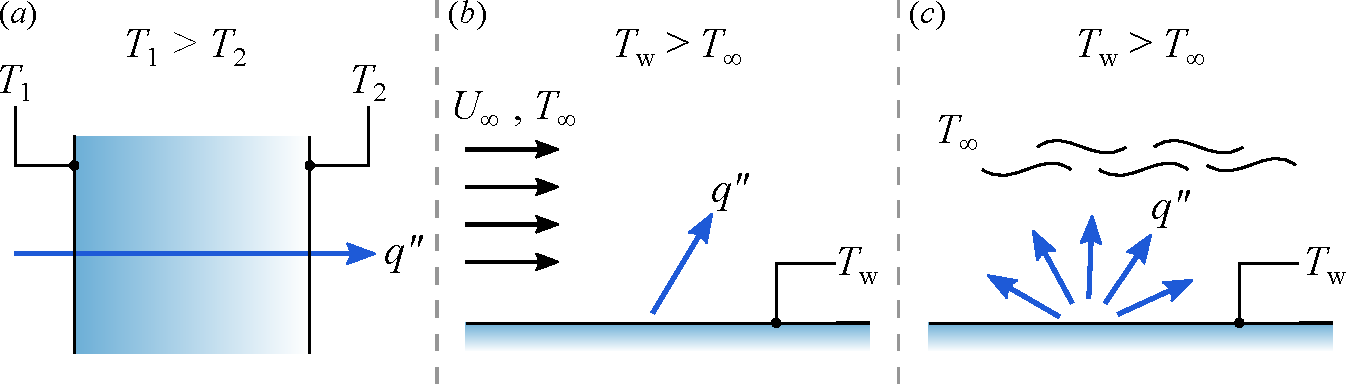
\includegraphics[width = 0.8\linewidth]{figures/dibujo_heat.pdf}
    \caption{Heat transfer mechanisms. (a) Conduction through a solid or a stationary fluid, (b) Convection from a wall to a moving fluid, (c) Radiation from a wall to the surrounding space. Figure adapted from \citet{bergman2011fundamentals}.}
    \label{fig:HTmethods}
\end{figure}

% Convection: the most complex
\citet{Gebhart1971HT} explains that the only physical mechanisms by which heat is transferred through and by the matter are conduction and radiation. However, if conditions occur in a moving medium, as is the case of fluids, the diffusion of thermal energy does not only happen at a microscopic level by the exchange of internal energy among molecules but also by the macroscopic motion of the moving medium. Eventually, this complex process is referred to as convection. Necessarily, convection becomes an additional heat transfer process to explain thermal energy transport in fluid flows. The study of convection includes all the mechanisms of conduction and radiation as well as those of the motion of fluids. Consequently, convection becomes the most challenging of the modes of transport within the field of heat transfer.

% Importance of heat transfer
Heat transfer gathers principles from thermal diffusion, electromagnetic radiation and fluid motion, including theories and knowledge from other branches of science. The study of heat transfer requires the mastery of many concepts and methods of analysis in several disciplines, with a crucial role in countless natural and industrial processes. The impact of thermal energy management on the current socio-economic environment is already discussed in Chapter~\ref{ch01}. Nonetheless, this is not a recent concern of modern science and engineering. In his communication to the Royal Society in 1852 (header of this chapter), Lord Kelvin concludes that there is a universal tendency in nature to the dissipation of mechanical energy, heat transfer being the mechanism driving this process. However, Lord Kelvin did not yet consider the dissipation of energy by convective heat transfer. 

%--------------------------------------------------------------------------------------------------
\subsubsection*{Heat transfer in fluid flows: Convection}

Convection is the heat transfer method of fluids par excellence. Depending on the nature of the fluid motion, convection may be classified into two different types. On the one hand, \textit{forced convection} occurs when the fluid motion is induced by external sources, such as a pump, a blower or the atmospheric wind. Forced convection is the predominant kind in both natural and industrial processes, as is the case of wall-bounded flows, jet shear layers or atmospheric flows. On the other hand, \textit{natural convection} happens when the motion is a direct consequence of buoyancy effects due to the temperature-induced density change within the fluid. A classic example of natural convection is the so-called Rayleigh–Bénard convection \citep{Bodenschatz2000RBC}.
%As an example, \citet{sanmiguelvila2016hconv} studied the onset of horizontal convection experimentally by differential heating on the bottom wall of an encapsulated fluid, and \citet{Shishkina2011Rayleight} applied model-free control strategies to control RBC in a two-dimensional domain. 
% From a flow-control standpoint,

This work focuses on the forced convection in wall-bounded flows, in which the mainstream exchanges energy with the wall surface, as depicted in figure~\ref{fig:dibujo_ThBL}. Two essential concepts are to be introduced, namely the boundary layer and turbulence. As defined in Chapter~\ref{ch01} and expanded in Chapter~\ref{ch04}, turbulence is a flow regime characterised by its nonlinear, chaotic and high-dimensional nature. Additionally, the \textit{boundary-layer} (BL) concept is the baseline of modern fluid mechanics, developed by Ludwig Prandtl in 1904 \citep{prandtl1904BL}. Upon the motion of fluid over a solid surface, a thin layer of air develops at the interface in which the fluid adjusts its velocity from that of the free stream to that of the solid. This region is characterised by strong velocity gradients along the wall-normal direction; hence, viscous effects dominate the flow. This region is commonly known as hydrodynamic, or velocity, boundary layer, and its thickness is denoted by $\delta$. 
Similarly, for incompressible flows, the thermal BL develops when the wall temperature $T_\mathrm{w}$ differs from that of the free stream $T_\infty$, inducing a temperature gradient normal to the wall. The development of velocity and thermal boundary layers is driven by momentum and thermal diffusivity, which are related by a dimensionless group named the Prandtl number ($\nPr$), which relates the kinematic viscosity $\nu$ and the thermal diffusivity $\alpha$ as
\begin{equation}
    Pr = \frac{\text{Momentum diffusivity}}{\text{Thermal diffusivity}} = \frac{\nu}{\alpha}
\end{equation}

The Prandtl number can be used to determine the relation between velocity and thermal BL thicknesses ($\delta$ and $\delta_t$, respectively). As illustrated in figure~\ref{fig:dibujo_ThBL}, for $\nPr >1$, $\delta > \delta_t$, meaning that the flow is dominated by the diffusion of momentum whereas for $\nPr < 1$, the flow is dominated by thermal diffusion so that $\delta < \delta_t$.

\begin{figure}
    \centering
    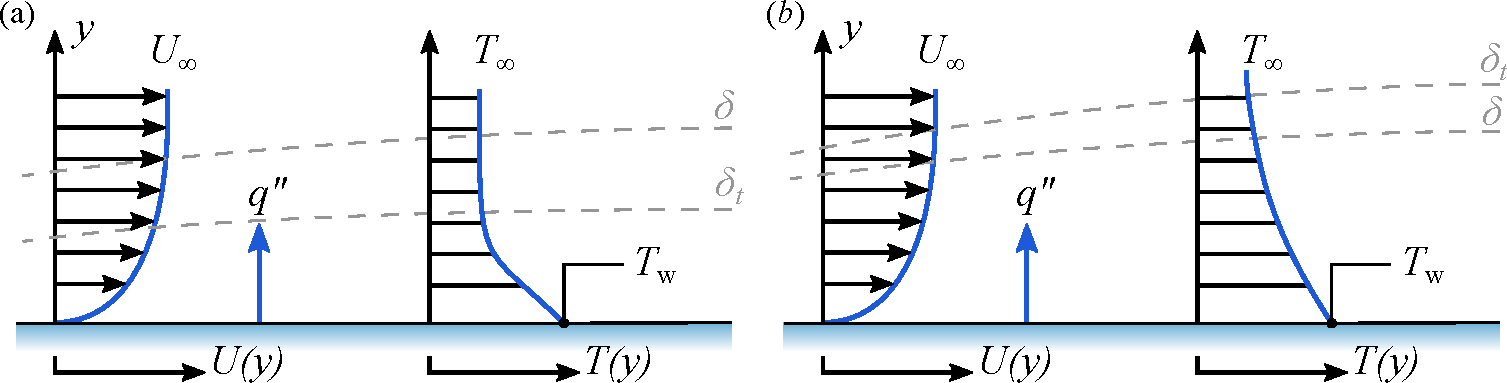
\includegraphics[width = 0.8\linewidth]{figures/dibujo_ThBL.pdf}
    \caption{Boundary layer development on a flat plate with convective heat transfer. (a) Thermal boundary layer thinner than the velocity boundary layer ($Pr > 1$); (b) Thermal boundary layer thicker than the velocity boundary layer ($Pr < 1$). The symbols correspond to wall-normal coordinate $y$, wall temperature $T_\mathrm{w}$, heat flux from the wall $q''$, and freestream velocity and temperature $U_\infty$,$T_\infty$, respectively.}
    \label{fig:dibujo_ThBL}
\end{figure}

Recalling the definition by \citet{Gebhart1971HT}, discussed above, convection is comprised of the energy dissipation due to random molecular motion and the bulk energy transfer due to the motion of the fluid at a macroscopic scale. These mechanisms are referred to as \textit{diffusion} and \textit{advection}, respectively. In turbulent boundary layers (TBLs), advection is dominated by the motion of coherent structures. From a thermodynamical perspective, coherent structures can be defined as fluid volumes moving collectively and with similar thermodynamic properties. The molecules composing the coherent structures retain their random motion through which diffusion is accomplished; hence the total thermal energy transport results from the superposition of random molecular motion on the microscopic scale and bulk fluid motion on the macroscopic scale. In other words, convective heat transfer is the cumulative effect of diffusion and advection. Diffusion is predominant in the near-wall region, where large eddies vanish into smaller scales dissipating energy. At the surface boundary, where the flow velocity adjusts to that of the wall, heat is transferred by diffusion only. The bulk energy transport is carried out by large structures within the boundary layer, exchanging heat with the free stream as well.

Regardless of the nature of the convection heat transfer process, the convective heat flux $q''~(\mathrm{W/m}^2)$ between the fluid and the boundary surface is determined from Newton's law of cooling, namely
\begin{equation}\label{eq:Newton_cooling}
    q'' = h(T_\mathrm{w} - T_{\mathrm{aw}})
\end{equation}
where the parameter $h~(\mathrm{W/m}^2\cdot\mathrm{K})$ is referred to as the convection heat transfer coefficient, and $T_{\mathrm{aw}}$ is the adiabatic wall temperature. The adiabatic wall temperature is a reference temperature of the fluid at which the heat transfer between the fluid and the wall is null. Its value depends on the flow conditions. For incompressible flows, as considered throughout this dissertation, the adiabatic wall temperature practically coincides with that of the undisturbed stream, i.e. $T_{\mathrm{aw}} \approx T_\infty$. Instead, for compressible flows, the reader is referred to \citet{Germain1955taw}, in which an extensive analysis and formulation are available.

Equating the heat conducted from the wall by the fluid by Fourier's law of thermal conductivity to the same heat transfer expressed in terms of a convection mechanism by Newton's law of cooling, the following relation is achieved:
\begin{equation}\label{eq:cond_conv}
    -k \left. \frac{\partial T}{\partial y} \right|_{y = 0} \equiv h(T_\mathrm{w}-T_\infty)
\end{equation}
where $k$ is the thermal conductivity of the fluid. The left-hand side in Eq.~\eqref{eq:cond_conv} represents the heat removed from the wall since no fluid flows through the wall. This relation can be expressed in dimensionless form as
\begin{equation}\label{eq:Nu}
    \left. \frac{\partial \left( \frac{T_\mathrm{w}-T}{T_\mathrm{w}-T_\infty}\right)}{\partial (y/\ell)} \right|_{y/\ell = 0} = \frac{h\ell}{k} \equiv \nNu_\ell.
\end{equation}
being $\ell$ a characteristic length of the flow under consideration, and $\nNu_\ell$ the Nusselt number based on $\ell$. The Nusselt number, as defined in Eq.~\eqref{eq:Nu}, may be interpreted as the ratio of heat transfer rate by convection to that of pure conduction through the medium. This dimensionless group is a classical form to refer to the convective heat transfer; however, it must not be mistaken with the Biot number ($\nBi = h\ell/k_\mathrm{w}$, being $k_\mathrm{w}$ the thermal conductivity of the solid wall), which is the ratio of the internal conductive resistance of a solid to the boundary layer convective resistance.

The study of convective heat transfer in fluid flows reduces to the determination of $h$. For experimental investigations, measuring heat fluxes at the wall requires both heat-flux sensors and temperature transducers. Papers 2, 3 and 5 in Part II of this manuscript, rely on the same methodology consisting of a heated-thin-foil sensor together with infrared thermography to acquire temperature. The heated-thin-foil is thermally thin \citep{astarita2012infrared}, i.e. it can be considered isothermal across its thickness since the Biot number is small for all the proposed problems ($\nBi < 0.1$). This non-intrusive measurement technique captures the distribution of convective heat flux on a surface. The interested reader is referred to the methodology section of Papers 2, 3 and 5 in Part II. 
%the Fourier number ($\nFo = \alpha_{s}/fs_{s}^2$, where $\alpha_{s}$ is the thermal diffusivity of the sensor, $s_{s}$ is the sensor thickness and $f$ is the IR camera sampling frequency, much larger than the inverse of the time scale of the phenomenon) is larger than unity; consequently, according to [20] the temperature distribution along the thickness of the printed circuit board is linear.
%-----------------------------------------------------------------------------------------
\subsubsection*{Analogy between Momentum and Heat Transfer}

The transport of momentum and energy in turbulent flows is based on similar mechanisms. The transport equations of these two quantities resemble each other. In their dimensionless form, the equations are analogous, depending on a few parameters, namely the Reynolds number \nRe, the Prandtl number \nPr, and the Nusselt number \nNu~(or the Stanton number \nSt, later introduced). There exist several versions of the momentum and heat transfer analogy. The most relevant are briefly described below, avoiding the mathematical process to obtain them for brevity. The interested reader is referred to the wide variety of textbooks on heat and mass transfer that cope with this topic \citep[\eg][]{bergman2011fundamentals,Lienhard2020}.

The first attempt to formulate this similarity was the famous Reynolds analogy. \citet{reynolds1874analogy} suggested that the concentration, velocity and temperature distributions should have a similar form, proposing a simplified mathematical rule that relates momentum and heat transfer processes.
\begin{equation}\label{eq:Re_analogy_aux}
    \frac{h}{\rho U_\infty c_p} = \frac{1}{2}\frac{\tau_w}{1/2\rho U_\infty^2}
\end{equation}

The right-hand side in Eq.\eqref{eq:Re_analogy_aux} represents the dimensionless representation of the wall shear stress $\tau_w$ (the Fanning friction factor $f = 2\tau_w / \rho U_\infty^2$), whereas the left-hand side of Eq.\eqref{eq:Re_analogy_aux} is a dimensionless group referred to as the Stanton number (\nSt) that measures the ratio of heat transferred to the fluid ($h$) to the fluid thermal capacity ($\rho U_\infty c_p$ being $\rho$ the fluid density, $U_\infty$ its velocity, and $c_p$ its isobaric specific heat). In other words, \nSt~describes the relationship between the heat transfer and the shear force at the wall, which translates into a geometric similarity between the velocity boundary layer and the thermal boundary layer. Hence, the Stanton number directly refers to $\nNu$, $\nPr$ and $\nRe$, relating momentum and thermal processes. The definition and physical interpretation of the Stanton number reads
\begin{equation} \label{eq:Stanton}
    \nSt = \frac{\text{Actual heat flux to the fluid}}{\text{Maximum possible enthalpy change}} = \frac{h\cancel{\Delta T}}{\rho U_\infty c_p\cancel{\Delta T}} = \frac{\nNu}{\nPr\nRe}
\end{equation}

Developing Eq.\eqref{eq:Re_analogy_aux}, Reynolds' analogy in its classical form reads as
\begin{equation}\label{eq:Re_analogy}
    \nSt = \frac{f}{2} \qquad \text{Reynolds analogy \citep{reynolds1874analogy}}
\end{equation}

Similarly, \citet{prandtl1910beziehung}, unaware of the pioneering work by \citet{reynolds1874analogy}, pointed out that the velocity and temperature differential equations are identical when the thermal and momentum diffusivities are equal. Both Reynolds' and Prandtl's analogies are valid for the simplified case of a boundary layer that develops on a flat plate under zero-pressure-gradient (ZPG) conditions and in the limit of $\nPr = 1$. Soon an unsuccessful attempt by \citet{taylor1916conditions} tried to formulate a generalized analogy for cases with $\nPr \neq 1$. \citet{colburn1933analogy} explored the relevance of the Prandtl number on the turbulent transport similarity. By combining energy and momentum transport equations within a turbulent boundary layer on a flat plate, the group $\nSt\nPr^{2/3}$ arises, which is defined as the $j$-factor. This analogy is an extension of classical Reynold's analogy, which is commonly known as the $j$-factor or Chilton-Colburn analogy \citep{Chilton1934Jfactor},
\begin{equation}\label{q:jfacto_analogy}
    \frac{f}{2} = j = \nSt\nPr^{2/3} = \frac{\nNu}{\nRe\nPr^{1/3}}
\end{equation}

The validity of these analogies is nonetheless restricted only to the boundary layer flow on a flat plate under ZPG conditions. Several authors aimed at developing more general models to relate heat and momentum transport; however, most of them rely on empirical coefficients or are case-dependent. For the reader's interest, an extensive review of heat-momentum analogies is presented by \citet{churchill1997critique}. %The above discussion is intended to present to the reader the concept of the heat and momentum transfer analogy, the principle of similarity between these two mechanisms and the definition of the Stanton number. Understanding these concepts enables exploring solutions for heat transfer control in other fields such as skin-fiction reduction, mixing enhancement or wake suppression. Furthermore, Paper 1 in Part II of this thesis leverages the Reynolds analogy to investigate an approach to reducing heat transfer in turbulent boundary layers.

%================================================================================================
%- Heat transfer control:
%================================================================================================
\section{Strategies for heat transfer control}

Heat transfer control is the discipline that explores thermal management strategies with the target of altering the mechanisms behind thermal energy transport. This discipline is commonly known as \textit{heat transfer enhancement} since most efforts are aimed at increasing the heat transfer capabilities of the system. Heat transfer enhancement is present in many industrial and research areas, such as space satellites' thermal management by radiation, conduction mechanisms in solar panels or convective heat fluxes in heat exchangers of engines. In this section, the focus lies on convective heat transfer control, performance quantification criteria, and the strategies to achieve enhancement. 

For an enhanced surface in single-phase flows, the ``basic performance characteristic'' is the $j-$factor from the Chilton-Colburn analogy, together with the friction factor, $f$, as a function of the Reynold number, $\nRe$. A straightforward possibility to quantify the performance enhancement is to calculate the ratios $j/j_0$ and $f/f_0$, where the subscript $0$ is for the reference condition. Although it depends on the enhancement strategy in use, commonly $f > f_0$ under the same $\nRe$. Thus, this approach does not accurately quantify the actual performance improvement, subject to specific operating constraints. Considering $j/j_0$ may yield unfair comparisons since the enhanced flow condition is allowed to operate at a higher pressure drop than the reference. In other words, the reference flow condition could achieve higher $h$ if operated at higher $\nRe$ to balance the pressure drop to that of the enhanced case. Therefore, the additional energy required to promote the enhanced heat transfer condition must be quantified to determine the performance fairly.

In the literature, there exist several measures of \textit{performance} for heat transfer enhancement strategies. It is worth noting that heat transfer enhancement is a discipline strongly related to the design, study and optimisation of heat exchangers. Based on the discussion by \citet{manglik2003heat}, the performance evaluation criteria (PEC) for single-phase flows strongly depend on the objective of the enhancement. A general formulation is proposed by both \citet{manglik2003heat} and \citet{webb2005enhanced} that relates the change in heat transfer coefficient $h$ for a heat transfer surface $A$ with the required pumping power $P$. This classical interpretation for heat transfer enhancement reads,
\begin{equation}\label{eq:PEC}
    \frac{hA/h_{0} A_{0}}{(P/P_{0})^{1/3}(A/A_{0})^{2/3}} = \frac{j/j_{0}}{(f/f_{0})^{1/3}},
\end{equation}
The general PEC is driven by the three variables on the left-hand side, namely ($hA/h_0A_0$), ($P/P_0$), and ($A/A_0$). By setting one of the variables as the objective, the remaining two are considered operating constraints, fixing their values to 1.0. In this work, the PEC in Eq.~\eqref{eq:PEC} is adjusted to the case of a turbulent boundary layer flow in which the thermal energy transfer process is mainly driven by a change in temperature between the mainstream and the wall. Consequently, the heating/cooling area and the Reynolds number are unaltered when applying the heat transfer enhancement technique, $A/A_0 = 1$. Therefore, the main objective of the herein considered problems is to control the value of $h$, while the power requirement is envisioned as a penalty term in the objective function. A deeper discussion on the formulation of the optimisation problem is provided in Chapter~\ref{ch03}.

The heat transfer control problem is then classified into different categories, depending on whether the objective is to enhance or reduce heat transfer and on the type of control strategy in use. For the latter, literature differentiates between \textit{passive} and \textit{active} techniques \citep[\eg][]{webb2005enhanced}. Passive flow control techniques are those that perform the actuation regardless of an external power supply. This is commonly achieved by geometry alteration of the surface such as roughness elements \citep{Hwang1995roughness,Hechuan2018ratchet}, obstacles \citep{mallor2018cubes}, riblets \citep{Mallor2019ribPOD}, or vortex generators \citep{Awais2018review,Ke2019VG}. Despite the undoubted effectiveness of passive elements, these devices are constantly present in the flow field, inducing a continuous pressure drop that translates into an undesired skin-friction augmentation. The inability to trigger the control action when desired or to adjust the control authority also deteriorates the performance of passive elements. Active control techniques cope with all the enumerated weaknesses at the cost of an external power supply to perform the actuation on the flow. There are countless active flow control devices such as continuous \citep{puzu2019jet} or synthetic \citep{Giachetti2018synjet} jets in crossflow, plasma actuators \citep{roy2008plasma}, electromagnetic forcing \citep{Kenjere2008EMheat} or moving walls by electroactive materials \citep{Leal2013rev_electroactive}, to name a few. Active control has gained interest in the flow control and heat transfer communities during the last decades due to its outstanding versatility in the control design, from the actuator to its control logic. Furthermore, the incursion of sophisticated algorithms into flow control triggers the possibility of exploring unconventional flow control strategies, adjusting their authority upon the requirements of the flow according to a pre-stated objective.

In this work, the focus lies on a specific mechanism through which heat transfer enhancement is achieved in turbulent flows, which consists of inducing streamwise vortices embedded in the boundary layer \citep{jacobi1995}. The resulting near-wall coherent structures prevail over a significant downstream distance, promoting cross-stream momentum transfer within the boundary layer. This actuation facilitates the transport of high-momentum fluid from the outer region towards the wall, exacerbating heat transfer and turbulent mixing. Classical, passive heat transfer enhancement methods exploiting this principle are wall-mounted obstacles and vortex generators. 
%For the latter, there are three basic recommendations to design the VG: longitudinal vortices are more effective than transversal vortices; (2) delta winglets outperform rectangular winglets; and (3) optimum angles of attack lies in the range $[30^\circ,45^\circ]$.
Vortex generators (VG) are widely used in the aeronautical industry as a passive element to promote turbulence transition on adverse-pressure gradient flows \citep{Lin2002reviewVG} and in heat transfer enhancement applications such as heat exchangers \citep{Awais2018review}.  Regarding wall-mounted obstacles, the work by \citet{Chyu1996obstacles} investigates the flow topology and heat transfer distribution around several obstacle shapes. A horseshoe vortex develops upstream with the corresponding streamwise counter-rotating vortex pair extending downstream at both sides. At the downstream side of the obstacle, the flow separates and recirculates, yielding a reduction of convective heat transfer at the wall. The flow re-attaches further downstream with an impinging flow known as the arch-shaped vortex. According to \citet{Chyu1996obstacles}, the cubes are the best shape for heat transfer enhancement purposes upstream of the obstacle. However, they present a strong recirculation area as demonstrated by \citet{nakamura2001cube}. \citet{mallor2018cubes} aimed to solve this issue by perforating the wall-mounted cubes similar to the perforated fins in channel flow used by \citet{Hwang1995roughness}. Perforated cubes not only reduce the recirculation region but also increase the maximum Nusselt number at the wall due to the impingement of the flow coming through the perforation. It is worth noting that the flow around an obstacle resembles that induced by other active elements as the jets in cross flow \citep{fric_roshko_1994}. A detailed description of jets in cross flow reads in section~\ref{ss:JICF}.

On the contrary, few contributions exist regarding heat transfer reduction in turbulent boundary layers. The early and extensive study by \citet{Moffat1984review} investigates a TBL when submitted to different perturbations such as acceleration, deceleration, roughness and surface curvature, among others. Although this study may seem obsolete, it pointed out several basic flow mechanisms to modify the Stanton number that have been later better explained and exploited for flow control, such as the opposition control \citep{Choi1994}. In that respect, the contributions in skin-friction drag reduction are counted by hundreds, which could be extrapolated to convective heat transfer reduction by invoking the analogy between momentum and heat transfer described above. Most effective flow control techniques to reduce momentum flux must interrupt the bursting cycle's self-sustaining regenerative process \citep{hamilton1995,Jimenez1999,schoppa2002}. Typically, the cycle envisions the generation of low-speed streaks by the lift-up effect of fast-advecting streamwise vortices \citep{Butler1993streak} within the boundary layer. Then, the transient growth of the streaks collapses in the regeneration of streamwise vortices \citep{hamilton1995,schoppa2002}. The so-called opposition control \citep[\eg][]{Choi1994,Stroh2015,Fukagata2003oppcontrol} is the most classical approach used to reduce skin-friction drag, which aims at damping coherent structures in the near-wall region. Another classical approach is the generation of embedded streamwise vortices within the turbulent boundary layer, as proposed by \citet{Schoppa1998}. A 20\% drag reduction in a turbulent channel upon generating large-scale counter-rotating streamwise vortices by wall jets. In contradiction to the above discussion for heat transfer enhancement, the large-scale swirl motion merges streaks into a larger streak envelope with reduced strength, thus cancelling the generation of streamwise vortices in the last part of the bursting cycle and reducing drag \citep{schoppa2002}. The heat transfer footprint of streamwise vortices embedded in a TBL is investigated by \citet{Zhang1993heatJICF}, concluding that those vortices that are deeply embedded with a reduced size and strength are the ones that could be used to reduce heat transfer and skin friction. Similar experimental investigations use jets vortex generators \citep{iuso2002} or body forces by plasma actuators \citep{cheng_wong_hussain_schroder_zhou_2021} to induce large-scale vortical motion that effectively reduces skin-friction drag.\\

The following sections provide a detailed description of the active flow control techniques used in this thesis. Plasma actuators are employed in Paper 2 to reduce heat transfer whereas jets in cross flow are tuned in Papers 3 and 5 to maximise the convective heat transfer.

%------------------------------------------------------------------------------------------
\subsection{Plasma actuators}\label{ss:PA}

The term \textit{Plasma} was first coined by \citet{Langmuir1928plasma} to denote an electrically-neutral ionised gas. Since then, the term plasma has been used in physics to define when substances feature charge equilibrium, generally known as the \textit{fourth state of matter}. Hence, plasma is a gaseous system of free-floating charged species that mutually interact, providing outstanding electromagnetic response of the plasma cloud and good electrical conductivity. The study of plasma and its applications have received overwhelming attention in the past, especially in flow control, space propulsion, material science and medicine, among others. The interested reader is referred to the extensive work by \citet{fridman2008plasma} to delve into plasma physics.

The production and preservation of a plasma discharge come hand in hand with several technological challenges due to the considerable energy requirement for promoting gas ionisation and the degradation of materials nearby the plasma cloud. The ionisation of a given volume of gas is usually achieved by applying an electric field, which is generated by either direct current (DC) or alternating current (AC) voltage. There is a minimum required voltage to sustain electron-ion pairs in the gas, the \textit{breakdown voltage} $E_b$, which depends on several factors like the driving frequency, the temperature and pressure of the gas, or the chemical composition of the gas \citep{Kunhardt1980breakdown,kunhardt1983electrical}. For the particular case at standard atmospheric conditions using air as a gas, the produced plasma is characterised by incomplete ionisation and no thermal equilibrium. Hence, the energy provided by the electric field is mainly stored in the free electrons, which translates into a relatively low temperature, given the name of \textit{cold plasma} \citep{Yamamoto2007plasma}. This kind of plasma is typically used in flow control applications as later proposed in this thesis.

The plasma actuators are devices that generate plasma to induce body forces in a specific manner. According to the extensive review by \citet{Kotsonis2015review}, plasma actuators are the modern technological implementation of Aristotle's concept of the \textit{unmoved mover}. The plasma actuator is a static device that can induce motion in the surrounding fluid without moving parts or the injection of a secondary stream. There are several alternatives for plasma actuators such as alternating current dielectric barrier discharge (AC-DBD) \citep{Roth1998dbd}, direct current corona (DC-corona) \citep{Leger2001corona}, nanosecond pulsed dielectric barrier discharge (ns-DBD) \citep{Roupassov2009nsplasma}, and arc filament actuators \citep{Samimy2004arcfilament}. In the following, only AC-DBD plasma actuators are considered, which is the kind used in this thesis.

\begin{figure}
    \centering
    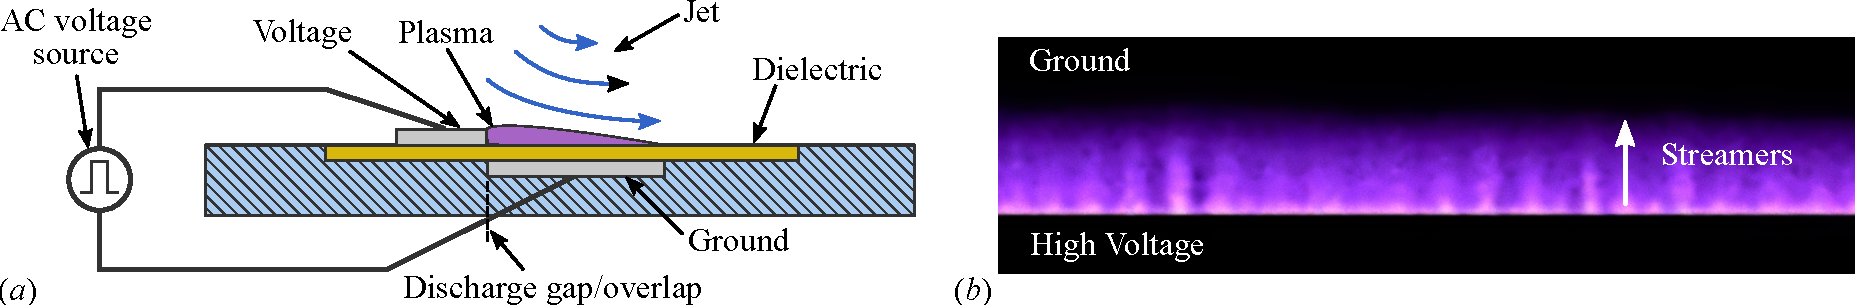
\includegraphics[width = 0.99\linewidth]{figures/schematic_plasma.pdf}
    \caption{AC-DBD plasma actuator. (a) Schematic of a typical cross-section of an asymmetric AC-DBD plasma actuator. (b) Top-view photograph of the purple glow on a DBD plasma actuator.}
    \label{fig:schematic_plasma}
\end{figure}

The specific dielectric-barrier-discharge configuration consists of two electrodes separated by a dielectric material. One of the electrodes is referred to as \textit{encapsulated}, which is commonly grounded and covered by the dielectric material. The remaining electrode is known as \textit{exposed}, since it is in direct contact with the surrounding fluid. The latter is connected to a high-voltage supply that is used to reach the breakdown voltage to generate plasma. Note, however that the opposite configuration with a high-voltage \textit{encapsulated} electrode and a grounded \textit{exposed} electrode is also possible. For a single plasma actuator configuration in which only one plasma plume is produced, the electrodes arrange as shown in figure~\ref{fig:schematic_plasma}(a). Upon the application of high voltage (HV), charge tends to accumulate on the surface of the dielectric material, yielding filamentary micro discharges, also known as streamers \citep{Kogelschatz2002filamentary} (figure~\ref{fig:schematic_plasma},b). These streamers change the capacitance of the dielectric barrier, reversing the local electric field and, thus, terminating themselves \citep{Eliasson1991streamers}. Based on this phenomenon, a continuous plasma discharge requires the application of variable voltage, either in the alternating or pulsating form \citep{michelis2017boundary}. Although the application of DC voltage is possible by substituting the dielectric barrier with a resistive barrier \citep{Laroussi2002resistive}, the most typical configuration of DBD actuators employs AC voltage, as shown in figure~\ref{fig:schematic_plasma}. For an AC-DBD plasma actuator working in air, the plasma is characterised by the back-and-forth motion of heavy ions, following the AC polarity inversion. This motion promotes collisions among the heavy-charged species (positive and negative ions), which results in a momentum exchange with the surrounding air \citep{Kotsonis2015review}. The resultant electric field and, thus, discharge are asymmetric due to the electrode arrangement. Consequently, the momentum exchange produces an uneven body force that directs from the exposed to the covered electrode, which induces a wall-tangent motion of the fluid. The resultant wall-jet structure, also referred to as \textit{ionic wind} \citep{Benard2014review}, injects fluid at a velocity which does not typically exceed $10\mathrm{m/s}$ \citep{Moreau2007review}.

Flow control strategies based on plasma actuators received much interest during the last few decades, still being very promising due to their electric nature. As the Aristotelian \textit{unmoved mover}, plasma actuators do not need movable parts to induce a fluid motion. At the same time, these devices feature a high-frequency response, being fully controllable in terms of amplitude and frequency within their operating limits. From a practical standpoint, plasma actuators require low power to operate, and their manufacturing is rather simple. In addition, they are very versatile in terms of geometrical patterns, extension, and thickness, which makes them very suitable to be flush-mounted devices with minimal flow disturbance while inducing body forces in the desired region direction and shape. Besides their control authority restricting their application to high Reynolds numbers, the aforementioned factors make DBD plasma actuators good choices for controlling aerodynamic flows such as laminar-to-turbulent transition \citep{Grundmann2008cancelTS,kotsonis2015control} and separation \citep{Little2010airfoilplasma,Michelis2015track}. A thorough summary of flow control studies based on DBD-plasma actuators is provided by the extensive reviews by \citet{Moreau2007review}, \citet{Corke2010}, \citet{Benard2014review}, and \citet{Kotsonis2015review}.

Plasma actuators have also been used to control the momentum fluxes within turbulent flows, especially for skin-friction reduction. A common approach consists of inducing spanwise travelling waves or spanwise oscillations. This strategy relies on the classic drag-reduction methodology proposed by \citet{Schoppa1998}, which aims at generating streamwise vortices embedded in a boundary layer to reduce momentum fluxes at the wall. In this regard, the experimental study of \citet{Whalley2014} employs a set of different plasma actuators to investigate the effect of co- and counter-rotating streamwise vortices in a turbulent boundary layer. They conclude that the formation of the spanwise travelling wave enables the formation of wide ribbons of low-speed streamwise velocity within the viscous sublayer, which locally reduces skin friction. Likewise, \citet{jukes2006TBLcontrol} achieved a strong skin-friction drag reduction downstream of the plasma actuator. These so-called ``plasma streamwise vortex generators'' (PSVGs) consist of a single or an array of plasma actuators aligned with the flow direction. Hence, the momentum injection by the actuators is normal to the mainstream, which leads to twisting and folding of the flow that eventually transforms into a streamwise vortex \citep{jukes2013plasmaVG}. The use of streamwise-aligned plasma actuators has been investigated in laminar \citep[e.g.,][]{jukes2013plasmaVG,serpieri2017} and turbulent boundary layers \citep[e.g.,][]{Jukes2006, Whalley2010DBDvortex, Wittig2019VGplasma} with promising results as a skin-friction drag reduction technique. 

Regarding heat transfer control, DBD plasma actuator applications are rather unexplored. It is worth noting that, despite the non-thermal nature of cold plasma, the plasma discharge locally produces thermal energy that may lead to a thermal footprint. Nonetheless, most of the produced heat diffuses through the dielectric and is not released to the fluid flow \citep{Rodrigues2018,Jukes2006}. The DBD plasma actuator proposed in this thesis resembles to that studied by \citet{Whalley2014}, \citet{Wittig2019VGplasma}, and, especially, \citet{cheng_wong_hussain_schroder_zhou_2021} (see figure~\ref{fig:dbd_actuator}). According to \citet{Wicks2015}, for opposing plasma discharges, streamwise vorticity generates upon the re-orientation of wall-normal vorticity from the actuators and spanwise vorticity from the boundary-layer, towards the streamwise direction. The reason behind this choice is that, contrary to conventional spanwise-aligned actuators, injecting momentum in the free stream direction to energise or weaken the boundary layer, the generation of streamwise vortices could potentially reduce turbulent fluxes at the wall. The research in Paper 2 thus aims at reducing convective heat transfer with an array of plasma actuators streamwise vortex generators. 

\begin{figure}
    \centering
    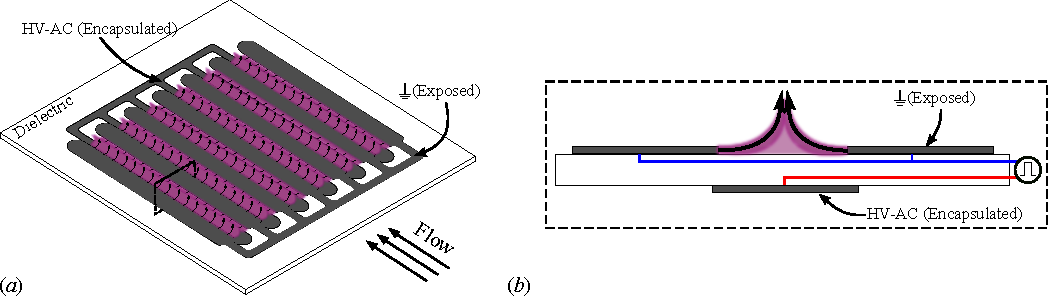
\includegraphics[width = 0.99\linewidth]{figures/dbd_actuator.pdf}
    \caption{Schematic representation of the DBD-plasma actuator array used in Paper 2. (a) Tri-dimensional representation of the array, and (b) cross-section of a pair of actuators.}
    \label{fig:dbd_actuator}
\end{figure}

As shown in figure~\ref{fig:dbd_actuator}, an array of DBD plasma actuators is considered in this thesis. Each actuator shares the encapsulated electrode with its adjacent. A total of 6 linear bi-directional actuators is used to ensure spanwise uniformity of the plasma-induced control. In this particular case, the air-exposed electrode is grounded while the encapsulated electrode beneath the dielectric material is connected to a stable high-voltage supply. As described in Paper 2 of this thesis, the actuator generates a sequence of opposing wall jets tangent to the surface in the spanwise direction, inducing pairs of counter-rotating streamwise vortices. In the recent study by \citet{cheng_wong_hussain_schroder_zhou_2021}, pairs of streamwise counter-rotating vortices are induced by plasma, merging with natural TBL streaks and interrupting the turbulence regeneration cycle, thus reducing skin friction. Invoking Reynolds' analogy of momentum and energy fluxes in turbulent boundary layers, the methodology proposed in Paper 2 exploits the same principles for an effective reduction of convective heat transfer in a turbulent boundary layer.

%------------------------------------------------------------------------------------------
\subsection{Jets in crossflow}\label{ss:JICF}

The jet in crossflow (JICF), or transverse jet, is a complex flow configuration present far and wide in natural processes and engineering applications. It is possible to find JICF in natural phenomena such as volcanic eruptions or the merge of a river and its tributary, although they are most commonly studied due to their relevance in the engineering field like for film cooling of turbine blades or thrust vector control for missiles, to name a few. Thus, the jet in crossflow can be adapted to the application, with several possible alternatives in nozzle size and shape, pulsation, inclination of the injection plane or injected fluid, for instance. The extensive field of application and variations of JICF requires a deep understanding of the flow topology, mixing, structural and sometimes reactive features to accurately design the operating and control conditions \citep{Karagozian2014revJICF}.

The utilisation of transverse jets for flow control is still an active research field with constant technological development and practical applications. It is well-agreed that a jet stream interacting with a crossflow provides better mixing capabilities than a free jet or a mixing layer \citep{kamotani1972experiments, broadwell1984structure}. The complex interaction of the jet flow with the freestream induces a web of flow structures and vortex systems that must be properly understood and managed for an effective flow-control purpose. The canonical configuration of a steady round jet perpendicular to a crossflow has been widely studied in the last decades \citep{kamotani1972experiments, fric_roshko_1994, kelso1996experimental, broadwell1984structure, smith1998mixing} due to its relevance in several engineering fields, especially in air-breathing engines. 

Following the seminal research work by \citet{fric_roshko_1994} and the extensive reviews by \citet{Mahesh2013revJICF} and \citet{Karagozian2014revJICF}, four main vortical structures are distinguished, as illustrated in figure~\ref{fig:JICF}. Upon the interaction of the freestream flow with the jet stream, small coherent structures develop in the form of ring-like vortices, commonly known as shear-layer vortices, which dominate the upstream formation of the jet column and are found to have the same direction of vorticity and similar length scales as the boundary layer formed inside the jet. These vortical structures are said to be formed from instabilities in the jet's shear layer, particularly on Kelvin-Helmholtz instabilities near the jet exit \citep{fric_roshko_1994, kelso1996experimental}. It is worth noting that the jet shear-layer instability found on free and transverse jets are significantly different in nature and formation characteristics \citep{megerian2007transverse}. Second, dominating the jet cross-section, a counter-rotating vortex pair (CVP) is produced in the near-field region of the jet \citep{kamotani1972experiments}. This large vortical structure is responsible for the pressure difference between the downstream and upstream sides of the jet exit and the vorticity evolution in the shear layer of the jet stream \citep{andreopoulos1984experimental, cortelezzi2001formation}. The formation of the CVP is attributed to the roll-up of vortex rings in the near-field region of the flow. The interaction among the vortex rings, as well as their roll-up and deformation, can be influenced by changes in flow conditions, such as the crossflow velocity, jet velocity and boundary layer thickness and have a significant impact on the entrainment of the crossflow into the near-field of the jet \citep{smith1998mixing,kamotani1972experiments,cortelezzi2001formation}. Third, a system of horseshoe vortices wraps around the jet base \citep{Krothapalli1990HSvort} due to the interaction between the mainstream boundary layer and the transverse flow exiting the jet \citep{kelso1995horseshoe}. These trailing vortices resemble those formed in flows around wall-mounted cylinders but can also oscillate and coalesce with other structures in the flow, leading to an unsteady regime under certain flow conditions \citep{kelso1995horseshoe}. Last, smaller-scale structures build up downstream of the jet column primarily attached to the wall and contain fluid of the wall boundary layer that entrains into the jet stream \citep{fric_roshko_1994}. The formation mechanism of the wake vortices is fundamentally different from those found in the flow around solid cylinders as the vortices are not shed directly from the jet but originate in the wall boundary layer. Periodic separation of the wall boundary layer caused by adverse pressure gradients induces an upward release of fluid and vorticity that generates column-like structures rising from the wall \citep{fric_roshko_1994}. These coherent structures contribute to the transverse jet's complex structure and mixing characteristics \citep{smith1998mixing}. The horseshoe vortex and the CVP, in particular, play a key role since they add to the mean flow while the wake and shear vortices mainly affect the fluctuating dynamics of the jet \citep{karagozian1986analytical}.

\begin{figure}
    \centering
    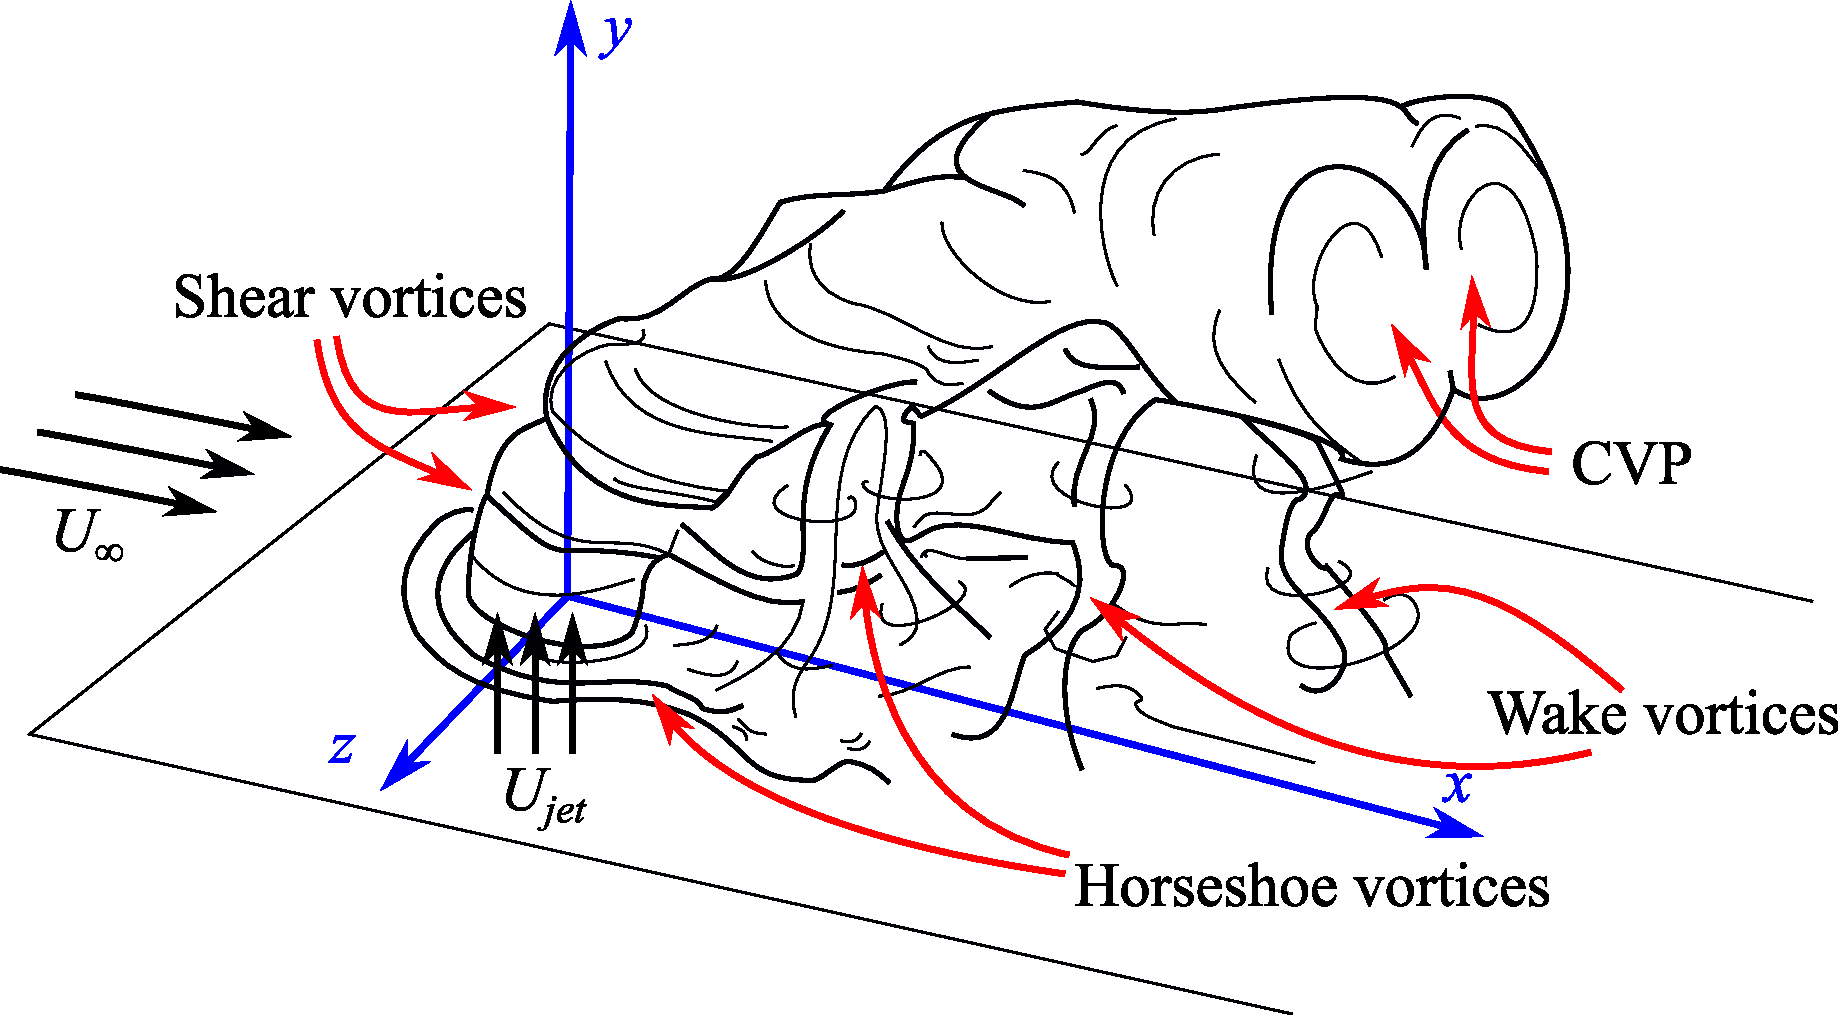
\includegraphics[width = 0.7\linewidth]{figures/JICF.pdf}
    \caption{Vortical structures for a round jet injecting steady fluid into a normal crossflow. Adapted from \citet{Karagozian2014revJICF}.}
    \label{fig:JICF}
\end{figure}

The mixing enhancement is the most common target when the JICF is used as a flow control actuator. This application is reported in the classic work by \citet{smith1998mixing}, which shows that the mixing enhancement narrows to the near-field region of the flow dominated by the CVP's structural formation and not to the far-field region where the CVP is fully developed. Regarding heat transfer enhancement applications, \citet{puzu2019jet} investigated the influence of the CVP and horseshoe vortices downstream of the jet injection. They report that the secondary mixing by the combined effect of the collapse of the CVP and the merge of the horseshoe vortices leads to a local convective heat transfer enhancement due to better entrainment and mixing within the boundary layer. Nonetheless, there is consensus that the pulsation or modulation of the JICF considerably improves its mixing performance compared to the steady jet. This matter is discussed in the experiments by \citet{vermeulen1992mixing, johari1999penetration, eroglu2001structure, MCLOSKEY2002, Johari2006scaling}, to name a few. \citet{vermeulen1992mixing} reported a considerable increase in the mixing area, penetration, and overall mixing by acoustically exciting a jet into a hot crossflow. They also concluded that the collapse of the structures and the interaction promoting mixing are displaced upstream, with higher mixing rates in the downstream vicinity of the injection. On the other hand, \citet{johari1999penetration} considered a fully-modulated JICF (valve-actuated) to study the effect of the frequency and duty cycle on the mixing properties, demonstrating that a short injection time (also referred to as pulse width) provides a higher mixing performance and dilution. The experiments by \citet{eroglu2001structure} and \citet{MCLOSKEY2002} focus on the induced perturbations on the vortical structures by the pulsation, finding that square-wave excitation generates distinct vortex rings. Most of the investigations of flow control with pulsed JICF agree on the importance of tuning the control strategy to find the optimal configuration that amplifies or optimises the desired flow feature \citep{shapiro2006optimization}. However, there is no universal objective function to drive the optimisation of pulsation due to the dependency on the flow and pulsation conditions, which are found to be apparatus-dependant \citep{MCLOSKEY2002}. The interested reader is referred to the extensive review article by \citet{karagozian2010transverse} covering the jet in crossflow and its control.

Besides the undeniable suitability of pulsed JICF for several flow control applications, there is still a profound lack of consensus on the flow structures, the dynamics and the correct scaling that characterise this flow configuration \citep{Sau2010optJICF}. The \textit{formation number} \citep{gharib1998scalingVR} is used in some studies \citep[e.g.][]{MCLOSKEY2002,shapiro2006optimization} to express the optimal pulsation condition, although this parameter was conceived for quiescent flows. \citet{Johari2006scaling} proposes the \textit{stroke ratio} and \textit{duty cycle} to scale the pulsed JICF together with a classification of induced structures such as hairpin vortices, vortex rings with or without trailing columns or turbulent puffs; nonetheless, \citet{Sau2008dynamicsVRICF} refuted this idea, demonstrating its validity just for quiescent flow conditions. The regime map suggested by \citet{Sau2010optJICF} builds upon two dimensionless parameters, namely the \textit{ring velocity ratio} and the \textit{stroke ratio}, gathering the effects of the pulsation frequency, duty cycle, modulation, and pulsed energy. For small ring velocity ratios, i.e. low injection velocities compared to the crossflow, the induced structures develop as hairpin vortices that progressively get closer as the stroke ratio is increased. There are two possibilities for high values of the ring velocity ratio: isolated vortex rings and vortex rings followed by a trailing column of vorticity, which depend on a low or high value of the stroke ratio, respectively. This map seems to reasonably fit with previous existing literature, showing that the optimal pulsation of JICF may be explained in terms of their vortex rings and that the optimal experimental conditions are seen to collapse on the same optimal curve. Howbeit, most of the engineering and technological studies that explore the utilization of pulsed JICF get behind the Strouhal number, $\mathrm{St}$, to characterise the modulation of the jet. In this regard, Paper 3 and Paper 5 of this thesis rely on the duty cycle and the Strouhal number as the scaling parameters to define the control action.

A simplified schematic of the pneumatic system used in Paper 3 and Paper 5 to generate the JICF is illustrated in figure~\ref{fig:schematic_pneumatic}. A pressurised air supply provides the jet stream. The air is filtered to avoid spurious oil or solid particles from entering the experimental setup. The control of the jet stream is performed in two steps. First, a pressure relief valve controls the absolute pressure on the system, which is always lower than that provided by the air compressor. This condition guarantees a constant operating pressure regardless of the jet actuation parameters. Second, a flowmeter and controller are used to monitor the flow condition, namely mass and volumetric flow rates, temperature, density and pressure. A settling chamber is used to prevent the flow meter and the pressure relief valve from spurious pressure waves induced by the ram effect at the solenoid valve. Eventually, a slot jet diffuser is used to progressively transition from a round shape of the pressurized line to the final rectangular shape at the jet exit.

\begin{figure}
    \centering
    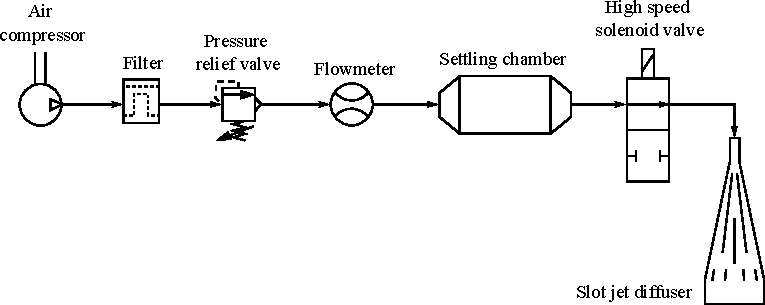
\includegraphics[width = 0.95\linewidth]{figures/schematic_pneumatic.pdf}
    \caption{Schematic of the experimental apparatus to control the jet in crossflow in the investigations of Paper 3 and Paper 5.}
    \label{fig:schematic_pneumatic}
\end{figure}

The dynamical behaviour and the flow topology of a non-circular JICF are very similar to those described above \citep{liscinsky1996crossflow, plesniak2005scalar}, especially in the far-field region of the flow. The interested reader is referred to the classic review by \citet{Gutmark1999noncirc}, where several investigations of flow control with non-circular jets are reported. In particular, the spanwise slot JICF has been investigated both experimentally and numerically for the steady-blowing configuration, and with jet modulation \citep[see e.g.][]{park1999, Krogstad2000slitjet, steinfurth2021CFslot}. The recent series of studies of pulsed slot jets in quiescent flow conditions \citep{steinfurth2020quiescentslot}, normal to a crossflow \citep{steinfurth2021CFslot}, and with an inclination angle of the injection plane with respect to the crossflow \citep{Steinfurth2021pulsedjet} shed some light on the flow structures for this kind of geometry. The flow configuration in Paper 3 resembles that investigated by \citet{Steinfurth2021pulsedjet}, in which the spanwise slot jet injects air at $30^\circ$ with respect to the wall. The inclination yields the jet stream to remain attached to the wall due to a Coand\v{a} effect and a local pressure deficit. A leading vortex develops downstream of the wall-attached jet, which eventually transforms into a half-ring vortex. On the other hand, the configuration used in Paper 5 looks like that in \citet{cheng2021skin} which combines several slot jets aligned with the freestream to promote skin-friction reduction in a turbulent boundary layer. 

\clearpage \newpage
\ \thispagestyle{empty}
%===============================================================================
\chapter{Control logic design}\label{ch03}
%===============================================================================
%
\begin{quote}
    \begin{flushright}
        \textit{Any sufficiently advanced technology \\
        is indistinguishable from magic.}\\
        \vspace{0.2cm}
        Arthur C. \citet{Clarke1968law3} \\
    \end{flushright}
\end{quote}
\vspace{1cm}

The design of the control logic and the formulation of the optimisation problem is described in this chapter. A brief introduction to model-base and model-free algorithms for flow control is provided, focusing on the two machine-learning-based algorithms used in this thesis: linear evolutionary algorithms and deep reinforcement learning.

\section{Turbulence flow control}

Turbulent flow control is a sub-field that intersects the study of turbulence and the application of control techniques. Three common strategies are found to control turbulence: aerodynamics shape optimisation, passive and active control. The reader is referred to Chapter~\ref{ch02} for an introduction to passive and active methods for heat transfer control in turbulent flows. Nonetheless, several other challenges are to be tackled, such as the proper selection of the flow control system (plant), meaningful sensing, the effective objective function or the control logic. In this following, a brief description of a general flow control problem is provided.

The mechanisms driving momentum and energy transports targeted by flow-control strategies greatly depend on the laminar or turbulent regime on which the fluid flow develops. Besides the appreciable understanding of turbulence, it is still hard to agree on a single, self-sustained definition of turbulence. The classic and complete definition by \citet{Bradshaw1971turbulence} reads,
%
\begin{quote}
    “turbulence is a three-dimensional time-dependent motion in which vortex stretching causes velocity fluctuations to spread to all wavelengths between a minimum determined by viscous forces and a maximum determined by the boundary conditions of the flow. It is the usual state of fluid motion except at low Reynolds numbers”.
\end{quote}
%
This rationale provides three main pillars upon which any turbulence flow control must build: the chaotic nature of turbulence, the existence of a wide range of scales in both space and time, and the three-dimensionality of the phenomena. Since the long-established study by \citet{Richardson1920}, and its extension by \citet{Kolmogorov1941}, it is well-known that the large-scale motion produces the energy that progressively flows through the spectral pipeline to the smallest eddies where it is dissipated into heat. In the particular case of a turbulent boundary layer, an effective control strategy to reduce turbulent fluxes tends to interrupt a self-sustained cycle involving near-wall turbulent structures \citep{hamilton1995,Jimenez1999, schoppa2002}, such as the opposition control for streak suppression \citep{Choi1994}. Hence, the cancellation or exacerbation of large-scale turbulent structures could effectively control physical phenomena such as reduction of skin-friction drag or heat and mixing enhancement.

The design of an optimal control strategy for turbulent flows is an ambitious venture. As discussed by \citet{cornejomacedaPhD}, there are three factors that affect the design of the turbulence flow control problem and its optimality:
%
\begin{itemize}
    \item \textbf{High-dimensionality}: the existence of a wide range of scales in time and space sets a strong requirement for flow reconstruction from simulation or experimental data. High time and space resolution data is required, rendering the problem sensing very costly;
    \item \textbf{Time-delayed response}: mainly related to the a non-negligible transient time between sensing and actuation command;
    \item \textbf{Frequency crosstalk}: modelling and predicting the flow becomes critical when there is a nonlinear interaction between modes.
\end{itemize}
%
Regarding the control logic, literature distinguishes between model-based and model-free algorithms. On the one hand, the model-based approach has shown its effectiveness when the flow control configurations can be modelled based on first- or second-order dynamics \citep{Rowley2006control}. Based on linear control theory, the main idea behind model-based algorithms is linearising the flow dynamics around a specific state of interest \citep{Kim2007linearcontrol,Sipp2010linearcontrol}. It is also common to project the dynamics on a reduced-order subspace composed of several dominant non-normal global stability eigenmodes \citep{akervik2007galerkin}. Some successful examples of model-based control are the opposition control \citep{Choi1994, Fukagata2003oppcontrol}, two-frequency crosstalk \citep{Glezer2005control,luchtenburg2009galerkin}, phasor control to stabilise oscillations \citep{pastoor2008control}, and quasi-steady response to quasi-steady actuation \citep{Pfeiffer2018robustcontrol}, to name a few. Notwithstanding, model-based approaches still grapple with turbulent flows, since linear control theory omits nonlinear interactions among modes \citep{BruntonNoack2015review}. Furthermore, the experimental investigation of turbulence control comes along with several technological constraints, such as the placement, quantity and type of sensors and actuators, which are regularly outlined from experience and engineering wisdom \citep{Cattafesta2011revFC}. The hitherto available measurement techniques provide a sparse representation of the flow state either due to insufficient time or spatial resolution. These additional constraints make model-based approaches often unpractical for in-time control \citep{cornejomacedaPhD}.

Model-free approaches, on the other hand, can derive optimised actuation commands for a certain flow configuration with a sparse representation of the state. These algorithms do not rely on any simplified or reduced-order model but consider the flow system as a black-box model that only attends to the actuation command and the sensor signals. Deriving optimal control laws based on model-free approaches is a complex enterprise, which requires the utilization of sophisticated regression techniques, based for instance on machine learning algorithms. Still, the non-convexity of the feasible solution space for the actuation design also challenges the model-free optimisation of turbulence control. In experiments, the problem is often simplified by selecting a reduced number of actuation parameters with adaptive variations either based on temporal evolution or sensor signal. Common model-free strategies for turbulence control are the evolutionary algorithms \citep{Koumoutsakos2001evolcontrol} and genetic algorithms \citep{Benard2016ga}, the extremum and slope-seeking control method \citep{Krstic2000extremumseek, Becker2007extseek, Gelbert2012extseek} and physics-based methods \citep{pastoor2008control,Zhang2004control}. 

The control logic proposed in the different analyses of this thesis is based on model-free approaches. The application of machine learning techniques to the field of fluid mechanics and flow control is a trending topic nowadays that continuously updates the state of the art. The comparative assessment presented in the Paper 4 of this thesis deals with two of the most prominent model-free control techniques from the machine learning literature, namely Reinforcement Learning (RL) \citep{sutton2018reinforcement} and Genetic Programming (GP) \citep{Koza1994gp}. On the other hand, the experimental flow control study described in Paper 5 employs linear generic algorithm control (LGAC) \citep{Benard2016ga} to find optimal open-loop control laws for heat transfer enhancement in a turbulent boundary layer. A brief description of the fundamentals of evolutionary algorithms and reinforcement learning is provided at the end of this chapter.

%------------------------------------------------------------------------------------------------
\subsection{Flow control as an optimisation problem}\label{ss:optproblem}
Solving the flow control problem based on a model-free algorithm is not a simple task. A common approach is to formulate it as an optimisation problem, in which the control law for each actuator is optimised based on a certain objective function while complying with either physical or technological constraints. The fluid system to be controlled, referred to as \textit{plant} from now on, is treated as a black-box model. The plant can represent several scenarios such as \citep{cornejomacedaPhD},
%
\begin{itemize}
    \item \textbf{Dynamical system}: defined as a system of equations, such as for instance the differential equations describing the Lorenz system.
    \item \textbf{Numerical simulation}: the computational resolution of a discretised system of equations, such as the Euler equations, the Reynolds Average Navier Stokes, or the direct numerical simulation of the N-S equations. This kind of plant usually provides a complete image of the flow state with no noise or disturbances affecting the sensing or actuation command.
    \item \textbf{Real fluid flow in a controlled environment}: the flow configuration is replicated in a controlled facility such as wind tunnels, free jets in a laboratory environment, channels, etc. The realistic environment of the experiment comes alongside external noise and disturbance affecting the flow state itself, as well as the measurements.
    \item \textbf{Real fluid flow}: direct testing of industrial applications such as a car, an aircraft, a heat exchanger or a jet engine in real-life conditions;
\end{itemize}
%
The control of the plant is achieved by the utilisation of actuators, whose number and type will strongly depend on the flow configuration and the target of the optimisation. In Chapter~\ref{ch02}, several actuators used in heat transfer control applications are introduced, especially those under consideration in this thesis: plasma actuators and jets in crossflow. Besides their working principle, all the actuators aim at disturbing the flow in a certain way to exacerbate or cancel out the desired effect on the fluid flow. The actuation command is a vectorial quantity, $\bm{b}(t) = (b_1, \ldots ,b_{N_b})^T$, with as many elements as the number of actuators under consideration $N_b$. When the actuation command is driven by feedback information of the state, the control is said to be of the \textit{closed-loop} kind; otherwise, the actuation is commonly based on fixed or time-dependent parameter with no system information, which is known as \textit{open-loop} control. Both approaches are explored in this thesis, the former in Paper 4 and the latter in Paper 5. 

The following formulation of the flow control problem is presented in its most complete form, considering feedback information $\bm{s}$, actuation parameters $\bm{\theta}$ and time-dependent functions $\bm{h}$. The sensing information is a vectorial quantity, $\bm{s}(t) = (s_1, \ldots ,s_{N_s})^T$, with as many elements as sensors in use $N_s$. On the other hand, the number of control parameters $N_p$ and time-dependent functions $N_h$ is fully dependant on the problem at hand. We define a control parameter $\theta_i$ as a constant quantity affecting the controller somehow as could be the frequency or the duty cycle of a modulated flow, for example. Regarding the functions $\bm{h}(t)$, they are used to refer to time-dependent information that does not depend on the sensing, as it could be harmonic functions of a certain phenomenon. The actuation command is related to these three vectorial quantities as follows,
%
\begin{equation}
    \bm{b}(t) = \bm{K}(\bm{s}(t),\bm{h}(t);\bm{\theta})
\end{equation}
%
The function $\bm{K}: \mathbb{X} \mapsto \mathbb{K}$  maps the input space $\mathbb{X}$, comprising the parameters, sensors and harmonic functions, to the control-law space $\mathbb{K}$. 

The optimal $\bm{K}$ derives from the optimisation of a certain objective function. In fluid mechanics, the targeted objective functions in flow control problems usually relate to the minimization of drag, mixing enhancement, heat transfer enhancement or separation control, to name a few. The goal of the control problem is defined in the cost function $J$, which commonly decouples on physical phenomena on the plant $J_a$ and a penalisation term of the required energy for controlling such phenomena $J_b$,
%
\begin{equation}
    J = J_a(\bm{b}) + \alpha J_b(\bm{b})
\end{equation}

The cost function is a scalar quantity that depends on the performance of the control. From an optimisation standpoint, the flow control problem becomes a minimisation problem in which the optimal control $\bm{K^*}$ yields the minimum value of the cost function $J$ over the search space $\mathbb{K}$. The relevance of the penalisation term in the cost function can be customarily tuned by the parameter $\alpha$. A large value of $\alpha$ prioresses the energy consumption required by the actuation, which commonly leads to low, or even negligible, control intensity. The correct balance between both terms depends on the flow configuration under consideration and is commonly based on experience and engineering wisdom. Thus, the flow control problem reads as follows
%
\begin{equation}\label{eq:Optproblem}
    \begin{aligned}
        \bm{K}^{*} = \underset{{\bm{K} \in \mathbb{K}}}{\arg\min}~~ J(\bm{K})
    \end{aligned}
\end{equation}

This optimisation problem is a non-convex optimisation problem, which could be interpreted as a regression problem of the second kind since the optimal solution is not known. The distinction between regression models of the first and second kind was first introduced by \citet{Fisk1967reg}. The regression problems of the first kind are those in which a full representation of the plant is assumed by a transfer function $\bm{P}$ so that it is possible to relate the response of all the possible actions for every state. Hence, the regression problem consists of inverting the model of the plant, $\bm{P^{-1}}$, achieving a direct mapping of the sensors and the actuation command. Conversely, the regression problem of the second kind does not assume any knowledge of the plant dynamics. Since the optimal solution is unknown, this kind of problem relies just on the control performance, namely the cost function $J$. The interested reader is referred to the long-established work by \citet{Fisk1967reg} for a deep description of the regression of the second kind, and to the thesis by \citet{cornejomacedaPhD} for a more friendly and visual description of both problems.

% %%%%%%%%%%%%%%%%%%%%%%%%%%%%%%%%%%%%%%%%%%%%%%%%%%%%%%%%%%%%%%%%%%%%%%%%%%%%%%%%%%
\section{Reinforcement Learning}

\textit{Learning by doing} is, surely, the most intuitive, simple and common way of learning in nature and society. Like a kid practising how to ride a bike or a lion training for hunting, Reinforcement Learning (RL) is a computational approach to interactive learning. The RL learner, known as the agent, learns a mapping function between observations and actions with the specific target of maximising certain reward. This is a \textit{trial-and-error} process, through which the agent determines the intrinsic nature of the phenomena under control and, somehow, predicts the expected reward upon future actions. According to the categories proposed by \citet{BruntonNoackKoumoutsakos2020}, reinforcement learning is considered a \textit{semi-supervised learning} approach. Contrary to supervised learning, in which the labelled data is available to train the model, semi-supervised learning only counts on partially labelled data or, in the case of RL, on the interactions of the machine with the environment.  

This section introduces the essential principles of RL, its elements and the considered algorithm for training are introduced in this section. The herein explanation is mainly retrieved from the pioneering work by \citet{sutton2018reinforcement}, and the recent reviews on RL applied to fluid mechanics by \citet{Garnier2021RLrev} and \citet{Viquerat2021RLrev}. The curious reader is referred to these literature contributions for a profound understanding of this matter.

%---------------------------
\subsection{Basic elements, principles, and mathematical foundation}\label{ss:RLbasic}
%
Reinforcement learning is a class of mathematical methods for problem-solving based on decision-making \citep{sutton2018reinforcement}, which involve the goal-directed interactions of an agent with the environment \citep{BruntonNoackKoumoutsakos2020}. This interaction splits into (1) the observations from the environment, (2) the application of an action based on the previous observations, and (3) the quantification of the performance. Although RL models the interactions with the environment as a Markov decision process, similarly to dynamic programming \citep{Bellman1952dyprog}, there is no need to model the dynamics of the environment.

The typical learning loop for RL is illustrated in figure~\ref{fig:RL_loop} and executes as follows \citep{Viquerat2021RLrev}:
%
\begin{itemize}
    \item Assume the time instant $t$ at which the environment is defined by its state $s_t \in \mathcal{S}$;
    \item the agent commands an action $a_t \in \mathcal{A}$ based on the observation of the current state, which could be a full $s_t$ or partial observation $w_t$ (subset of $s_t$, taken from sensing for instance);
    \item the environment evolves from $s_t$ to $s_{t+1} \in \mathcal{S}$ upon the action of the agent;
    \item the agent receives a reward $r_t \in \mathcal{R}$ for the previous actuation, and a new observation $s_{t+1}$ (or $w_{t+1}$).
\end{itemize}
%
\begin{figure}
    \centering
    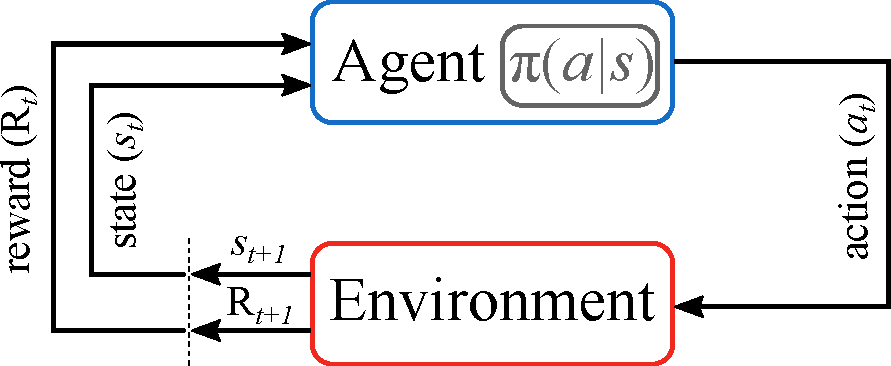
\includegraphics[width = 0.6\linewidth]{figures/RL_loop.pdf}
    \caption{Schematic of the typical learning loop for reinforcement learning agent. [Adapted from \citet{sutton2018reinforcement}]}
    \label{fig:RL_loop}
\end{figure}

In the previous description of the learning loop, $\mathcal{S}$, $\mathcal{A}$, and $\mathcal{R}$ correspond to the set of states, actions and rewards, respectively. These steps correspond to one cycle of the learning loop. The learning process extends for several cycles until a termination state is reached. The succession of cycles provides a repertory of actions and state observations ($s_t$ from now on for simplicity) that define a trajectory $\tau = (s_0,a_0,s_1,a_1,\dots)$. For each state, the agent looks for the optimal action to maximise its cumulative reward along the whole trajectory. In general, the targeted quantity is the discounted cumulative reward along a trajectory \citep{Viquerat2021RLrev}, defined as:
%
\begin{equation}
    R(\tau) = \sum_{t=0}^T \gamma^t r_t,
\end{equation}
%
where $T$ is the final time of the trajectory, and  $\gamma \in [0,1]$ is a discount factor to balance the relative importance of present and future rewards. The expected return is maximised through two possible approaches, namely value-based and policy-based methods. The former consist of determining the \textit{value function} \citep{sutton2018reinforcement} of a state-action pair, which is used to derive the following action to take at each state, while the latter directly aims at optimising a parameterised policy, which drives the agent performance.

A particularly successful application of RL is the resolution of games. The pioneering effort by \citet{Tesauro1992difflearn} describes a backgammon learner, in which the program started from no knowledge and trained by playing. After a million iterations, the program reached a performance similar to the best three human players in the world and won the computer backgammon olympiad \citep{BruntonNoackKoumoutsakos2020}. Recently, the development of neural networks allowed the application of RL to more complex games, such as Go \citep{mnih2015DRL} and the AI gym \citep{mnih2015DRL,Silver2016go}. RL is, however, a costly method due to the long learning process required to reach good performance. The acceleration of the learning process is a must for the application of RL to demanding scenarios, such as experiments and simulations of fluid flows \citep{Verma2018swimDRL}.

The agent does not only focus on revealing patterns in the environment dynamics or its actions but also aims at maximising the long-term rewards, which is the ultimate objective of RL methods. The long-term credit assignment (LTCA) implies assuming a certain relation between agent actions and environment rewards, which is derived from the trajectory of states and actions $\tau$. LTCA is still a major concern in RL. A common solution consists in modifying the original sparsely rewarded objective by adding highly rewarded sub-objectives \citep{schaul2015app}. Another challenge of RL is the correct use of information from experience by the agent when updated during the learning process \citep{Novati2019gliding}. In this regard, a proper tuning between \textit{exploration} and \textit{exploitation} is recommended. The agent must be able to find the optimal action by exploiting past experience while exploring alternative actions within the available solution space. Nonetheless, this is a common problem of several model-free algorithms.\\

Deep reinforcement learning (DRL) emerges from applying deep neural networks to model the agent. An artificial neural network (ANN), or simply neural network (NN), is a network of connected computational units, known as neurons, distributed in different layers that provides universal approximation capabilities \citep{Hornik1989MLP,Siegelmann1995NN}. For a fully connected network, each neuron receives input from all the neurons in the previous layer and feeds to all the neurons in the following layer. The neurons first compute the weighted sum of their inputs and, then, add a bias, which accounts for the output features that are independent of the input data. Eventually, the result from each neuron passes through a non-linear activation function that determines whether and to what extent the calculated value influences the final output. In DRL, NNs are trained to effectively map the relation between observations and actions \citep{rabault2019DRL}. This training process consists of the progressive adjustment of the biases and weights of the neural network towards the minimisation of a well-posed loss function that quantifies the network performance. The interested reader is referred to \citet{Goodfellow2016book} throughout the description of DRL.

In fluid mechanics, DRL has been recently applied to several problems to determine the parameters of control laws, such as swimming of fish schoolings \citep{gazzola2014RL}, control of unmanned aerial vehicles \citep{bohn2019DRL}, and optimization of glider trajectory taking ascendance \citep{reddy_learning_2016}. Most recently, DRL has been also applied to feedback-loop flow control like the wake control of a cylinder in simulations \citep{rabault2019DRL,rabault2019JFM} and in experiments \citep{Fan2020}, the tuning of the heat transport in a two-dimensional Rayleigh–Benard convection \citep{Beintema2020controlRBC}, and the wake stabilization past a cylinder by imposing a rotation on two control cylinders located at both sides \citep{Xu2020joh}.

\subsection{Policy-based methods} \label{ss:policymethods}
%
Policy methods rely on a \textit{policy} to drive the decision-making process of the agent. The final goal is to optimise the policy to maximise the expected discounted cumulative reward. The policy $\pi(a|s)$ is a mapping function based on a probability distribution over actions given a state rather than on a value function. Compared to value-based methods, policy-based methods ensure a better convergence, deal with high-dimensional action spaces, and exhibit great capabilities for learning stochastic policies \citep{Viquerat2021RLrev}. 

In fluid mechanics, most of the up-to-date applications of reinforcement learning prefer policy gradient methods, in which the parameterised policy $\pi_\theta(a|s)$ is optimised through a gradient ascent algorithm. The optimisation problem builds around the objective function, which is generally based on the expected discounted cumulative reward,
%
\begin{equation}
    J(\theta) = {\underset{\tau \sim \pi_\theta}{\mathbb{E}}}\left[ R(\tau) \right]
\end{equation}
%
to find the optimal set of parameters $\theta^*$ that maximises $J(\theta)$, namely
%
\begin{equation}
    \theta^* = {\underset{\theta}{\arg\max}}~{\underset{\tau \sim \pi_\theta}{\mathbb{E}}}\left[ R(\tau) \right]
\end{equation}

The optimisation problem could be directly solved by gradient ascent algorithm, considering an estimation of the policy gradient $\nabla_\theta J(\theta)$. The gradient with respect to the policy parameters $\theta$ is, however, a complex quantity to be determined. The common approach follows the log-probability trick \citep{Williams1992ML}, which derived $\nabla_\theta J(\theta)$ as an expected value that can be evaluated:
%
\begin{equation}
    \nabla_\theta J(\theta) = {\underset{\tau \sim \pi_\theta}{\mathbb{E}}}\left[ \sum_{t=0}^T \nabla_\theta \log(\pi_\theta(a_t|s_t)) R(\tau) \right],
\end{equation}

The evaluated gradient updates the policy parameters ($\theta \leftarrow \theta + \lambda  \nabla_\theta J(\theta)$, being $\lambda$ the learning rate) and the process repeats until convergence. The performance of policy gradient methods is jeopardised by the learning rate, which determines the step size in the gradient direction \citep{Viquerat2021RLrev}. Low learning rates translate into a long training process with no practical convergence whereas an excessive value of the learning rate could pass without heeding through the global optima, collapsing in a sub-optimal policy with poor performance. Proximal policy optimization \citep[PPO,][]{schulman_proximal_2017} relies on an effective heuristic to avoid destructive updates of the policy, i.e. it ensures restrained updates of the policy $\pi_\theta$, with respect to the previous $\pi_{\theta_{\text{old}}}$. The PPO method has drawn a lot of interest in the DRL community because of its increased learning stability and generally stable behaviour concerning hyperparameters. In fluid mechanics, early attempts to apply DRL for flow control focused on the simple problem of a shedding wake of a cylinder in simulations \citep{rabault2019JFM} and in experiments \citep{Fan2020}.

%------------------------------------------------------------------------------------------------
\section{Evolutionary Algorithms}

Optimization (and search) algorithms could be defined as learning algorithms featured by the determination of a probability distribution containing the relevant design aspects to optimise a given environment phenomenon \citep{BruntonNoackKoumoutsakos2020}. This conception was first envisioned by \citet{Schwefel1977}, introducing the concept of evolution strategies (ES) that later expanded to genetic algorithms \citep[GAs,][]{holland1992adaptation} and genetic programming \citep[GP,][]{Koza1994gp}, giving rise to the category of Evolutionary Algorithms (EA) in computational intelligence. Evolutionary algorithms or strategies build on the adaptation and progressive improvement of a set of candidate solutions inspired by biological evolution. Each potential solution is defined as an \textit{individual}, composing the \textit{population} that progressively evolves from one generation to the next. Darwin's ``evolution of species'' theory and its most recent updates and corrections describe the natural mechanisms governing the adaptation capability of individuals. The three main working principles of evolutionary algorithms derive from this knowledge \citep{duriez2017book,cornejomacedaPhD}, namely 
%
\begin{itemize}
    \item \textbf{survival of the best}: the most fitting or most performing individual, based on the environment requirements, prevails in the following generation. This mechanism guarantees the quality of incoming populations;
    \item \textbf{crossover}: mechanism to diversify the population by recombining individuals, which exploits the most performing features of the individuals;
    \item \textbf{mutation}: purely exploitative mechanism in which new individuals or features come up, ensuring uniqueness and freshness in following generations.
\end{itemize}
%
The recombination and mutation of individuals is a stochastic mechanism that guarantees the continuous exploitation and exploration of the most performing individuals within the solution space. Therefore, evolutionary algorithms may be thought of as crossbreeds between Monte Carlo sampling techniques, which explore the search space, and gradient search strategies, which exploit the best features toward a minimum.

Evolutionary algorithms can be used for flow control applications solving the optimisation problem in section~\ref{ss:optproblem}. The performance of each control law described by each individual is modelled by the cost function $J$ and the generation of individuals depends on the input data and the kind of algorithm. Under the umbrella of evolutionary algorithms, there is a wide variety of techniques to solve different types of problems. Some well-established examples are the genetic algorithms (GA) \citep{holland1992adaptation}, covariance matrix adaptation evolution strategy \citep{Hansen1996cmaes} or genetic programming (GP) \citep{Koza1994gp}. In this thesis, both GP and GA are considered in Papers 4 and 5, respectively. Both techniques stand on the same principle, mimicking natural processes; however, the definition of the individuals is different. GA identify the optimal individual as the best set of control parameters within the solution space, whereas GP derives a control law as a function of the input data, namely the sensor information. The control law provided by GP is commonly more complex and variable in time since it adjusts based on the state of the plant. GP represents a potent regression approach capable of re-discovering and combining flow control techniques without the need for physics knowledge in the circumstances of multi-frequency forcing and direct feedback control \citep{cornejomaceda2019pamm}.

GAs have been recently used to reduce the skin-friction drag in a TBL by optimising the phase delay among six streamwise-aligned slot jets \citep{Yu2021GA_drag_slot_jets},  to control the wake of a bluff body based on multi-frequency forcing \citep{minelli2020lgac}, and to optimise the performance of a spiral double-pipe heat exchanger \citep{Tian2020GAheatexchanger}, to name a few. In the field of heat transfer, the extensive review by \citet{Gosselin2009GareviewHT} describes many other successful applications of GA control. On the other hand, GP derives laws of low to medium complexity, such as the phasor control, threshold-level based control, periodic or multi-frequency forcing, including jet mixing optimization with pulsed jets at the nozzle exit \citep{zhou2020artificial}, drag reduction past bluff bodies \citep{li2019prf}, shear flow separation control \citep{gautier2015MLC}, reduction of vortex-induced vibrations of a cylinder \citep{Ren2019pof}, mixing layer control \citep{Parezanovic2016jfm}, and wake stabilization of complex shedding flows \citep{raibaudo2019pof}, among others.\\

The following section focuses on genetic programming, in particular in the Linear-based Genetic Programming (LGP) algorithm proposed by \citet{li2017GP} due to its greater degree of complexity compared to a classic GA. A brief description of the method and the learning process is provided. The interested reader on GAs is referred to \citet{holland1992adaptation} and \citet{Wahde2008book}.

\subsection{Genetic Programming}\label{ss:GP}
%
Genetic programming is an optimisation algorithm that proposes solution candidates as a computer program \citep{Koza1994gp}. These programs define the solutions in the form of a mathematical function of the input data, which could be used for several purposes such as fitting a surface, control laws or conditional decision making. In this section, this method is briefly introduced based on \citet{Wahde2008book}, \citet{duriez2017book} and \citet{cornejomacedaPhD}.

The internal representation of the mathematical function describing the control law is crucial to correctly applying the genetic operators. The classic classification distinguishes
%
\begin{itemize}
    \item \textbf{tree-based genetic programming}: the control law builds on a tree in which the nodes are the operators and the leaves are the operands \citep{duriez2017book}.
    \item \textbf{linear genetic programming (LGP)}: the control law is defined as a sequence of unitary or binary mathematical operations encoded in a matrix \citep{brameier2007linear}.
\end{itemize}
%
Despite sharing the same fundamental principle of operation, LGP is preferred in this thesis for its simplicity regarding multiple-input-multi-output (MIMO) control, since LGP deals with different input data and defines several control laws with only one matrix, and genetic operators, because mutation and crossover operations apply on the same matrix with simple combination or modification of individuals.

Linear genetic programming control (LGPC) is the application of LGP to solve control problems, deriving control laws as mathematical functions of the input data. The individuals, namely the control laws, are defined based on instructions, a register of variables and a set of constants \citep{duriez2014MLC}. The instructions combine input data through basic operations $(+,-,\times,\div,\sin,\text{exp},\text{\etc})$ to produce the control commands as outputs. Each individual, and its instructions, are represented by a 4-column matrix in which every row corresponds to an instruction. Columns 1 and 2 contain the register indices of the arguments, column 3 is the operator index, and column 4 is the output register. The registers are crucial in terms of memory management, distinguishing two types: \textit{variable registers} that can be overwritten during the execution of an instruction, commonly employed for intermediate calculations; and \textit{constant registers} that are preserved while the algorithms access the matrix data, which contain data of the problem or random constants. A potential problem of the matrix representation of the individual is the repetition of the same mathematical function after applying all the instructions, i.e. there is no unique matrix representation for a certain control law. A numerical test is performed before the evaluation of individuals in which repeated instances are discarded and replaced by a new one.

The combination of arguments and operators may yield instructions without any impact on the resultant control command, which is named \textit{introns}. These introns become crucial in the process of building relevant structures \citep{cornejomacedaPhD}. Nonetheless, the crossover and mutation operators may `activate' these instructions leading to an alteration of the resultant control law \citep{duriez2017book}. In principle, any mathematical function could be represented in matrix form if a sufficient number of instructions is considered together with a proper diversity in the operators' library. Not only that, but the library of input data plays a key role when building the proper control law. Eventually, the diversity of both libraries determines the complexity of the feasible solution space in the optimisation problem. \\

The LGPC process is described in the following as illustrated in figure~\ref{fig:GPC_algorithm}. The first step consists of a Monte Carlo optimisation through which a random sampling of individuals is used to generate the first population. Then, a tournament selection is carried out on the most performing individuals on which the genetic operations are performed to build the new generations. This process is repeated till convergence or when the stropping criterion is reached. Replication and elitism ensures the memory of the learning process while crossover and mutation exploit and explore over the solution space. The operator is chosen based on their respective probabilities ($P_c,P_m,P_r$), which are user-defined parameters that can be tuned to strengthen either the exploration or exploitation nature of the algorithm.

\begin{figure}
    \centering
    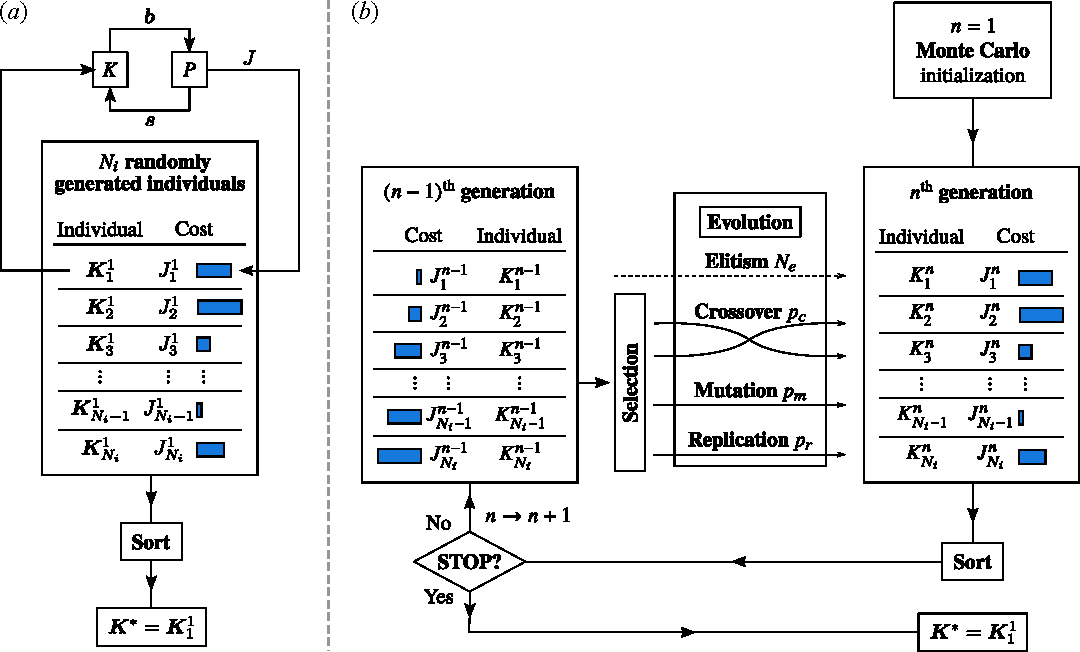
\includegraphics[width=0.99\linewidth]{figures/GPC_algorithm.pdf}
    \caption{(a) Monte Carlo sampling of the first generation. (b) Linear evolutionary algorithm. Each generation is built from the previous based on the genetic operators. \textit{Figures reproduced from \citet{cornejomacedaPhD} with permission of the author.}}
    \label{fig:GPC_algorithm}
\end{figure}

\subsubsection*{Monte Carlo optimisation}
Monte Carlo optimisation could, in principle, solve the flow control without the need for the evolutionary part; however, for a solution space with infinite dimensions, a multitude of individuals is required to ensure convergence toward the global optimum of the problem. LGPC considerably reduces the number of evaluations required for convergence, which becomes a limiting factor in real-life applications. The Monte Carlo optimization process provides the $N_i$ individuals of the first generation in the LGPC process by a random selection of operators and input data from the available libraries. Figure~\ref{fig:GPC_algorithm}(a) illustrate the Monte Carlo process for controlling a plant $P$ with the control law $K$ and control command $b$ (the reader is referred to section~\ref{ss:optproblem} for the definition of symbols). The maximum number of instructions and the number of variable and constant registers are user-defined parameters that the Monte Carlo sampling needs to comply with. The individuals are then evaluated and sorted based on their cost $J$. Eventually, the outcome of the algorithm is the most performing individual, i.e. the individual with the lowest cost.

\subsubsection*{Selection}
The genetic operations to build the incoming generations are performed on a certain set of individuals selected in a tournament selection process. The best $N_t$ individuals in the population are selected. The one that performs the best among them is picked with a probability of $P_t$. If not chosen, the same probability $P_t$ is used to select the second best and the process is repeated if needed for all the tournament individuals until the selection of the least performing. The user-defined parameters $N_t$ and $P_t$ influence the so-called \textit{selection pressure}, which is the degree to which high performers are chosen over low performers \citep{Wahde2008book}. Papers 4 and 5 in this thesis, for GP and GA respectively, follow the recommendations from \citet{duriez2017book}, setting $N_t = 7$ for a population of $N_i = 100$ individuals and $P_t = 1$.

\subsubsection*{Crossover for exploitation}
Crossover recombines individuals to extract the relevant features in the population. Thus, this is an exploitation operator through which two matrices split in two and swap, yielding two new individuals, namely the \textit{offsprings}.

\subsubsection*{Mutation for exploration}
The mutation is an exploitative operator to explore other features for a better control law. Each instruction has a certain probability to be randomly modified, which changes the matrix and, hence, leads to a new individual.

\subsubsection*{Replication and elitism for memory}
The most relevant features within a population are to be maintained for the incoming generation. Replication is the operator that copies individuals, ensuring the reminiscence of good individuals while enabling their future recombination. Similarly, the most performing individual during the process is always present in the latest generation due to elitism operator, preventing the loss of talent throughout the generations.

%
%===============================================================================
% Main contributions and Conclusions
%===============================================================================
%
%===============================================================================
\chapter{Main contributions and conclusions}\label{ch04}
%===============================================================================
%
The control of turbulence is a trendy research field with a potential expansion during the last decade thanks to the technological development hand in hand with novel algorithms based on artificial intelligence. This thesis aims at answering some of the numerous research questions within this exciting research area. This chapter gathers the main contributions and conclusions of the scientific publications performed in fulfilment of the objectives of this dissertation. For a more profound understanding and a detailed discussion of the results, the reader is referred to the appended papers in Part II of the present document.

The research work under the scope of this thesis deals with the control of turbulent boundary layers to manage the convective heat transfer at the wall. Starting from the exploration of well-known actuation mechanisms in other applications, such as skin-friction reduction or mixing enhancement, two parametric studies were performed to shed light on the flow mechanisms behind wall heat fluxes. As described in Chapter~\ref{ch02}, among the variety of available actuation systems, both plasma actuators and jets in crossflow were considered. In paper 2, a spanwise array of streamwise DBD-plasma vortex generators is used to reduce heat transfer. The experimental results confirm a considerable alteration of the flow topology due to the formation of pairs of counter-rotating streamwise vortices embedded in the boundary layer. An effective 10\% reduction in convective heat transfer is achieved. On the other hand, the spanwise slot jet in Paper 3 is used to enhance heat transfer. After the parametric study on the pulsation parameters, a simplified model is proposed decoupling the effect of the carrier frequency and duty cycle. A characteristic frequency of the system is found at which heat transfer enhancement is magnified. Although the justification of the optimality remains an open research question, flow field measurements revealed the development of large-scale turbulent structures in the near-wall region, which promote entrainment and mixing, hence enhancing heat transfer.

Seeking a more sophisticated control logic, the performance of machine-learning-based algorithms is evaluated in Paper 4. This article compares deep reinforcement learning and linear genetic programming control on a benchmark problem to assess their performance when varying the initial condition provided to the controller and in the presence of noise. In general, DRL outperforms LGPC; however, LGPC achieves significantly more compact and interpretable control laws, identifying subsets of the probes as being relevant to defining control actions. The numerical investigation concludes that RL and LGPC are up-and-coming flow control techniques, although LGPC seems more robust and implementable for practical applications. Based on this gained experience, Paper 5 deals with an experimental TBL control for heat transfer enhancement in which the control logic is given by linear genetic algorithms. The open-loop control problem can find the same characteristic frequency as in Paper 3, which corroborates its importance to maximize heat transfer.

%===============================================================================
%- Paper Highlights
%===============================================================================
\section{Paper highlights}
%-------------------------------------------------------------------------------
This section highlights the contributions of each of the papers included in the present thesis.\\

\noindent {\bf  Paper~1. Methodological.} \\
\noindent {\sc  Castellanos, R., Sanmiguel Vila, C., G\"uemes, A. \& Discetti, S.}{, 2021. }{\it  \let \\=~On the uncertainty of boundary-layer parameters from Ensemble PTV data . }{{Meas. Sci. Technol.}}{ {\bf  32}}{ (8)}{, 084006}.

\begin{itemize}
 \item An uncertainty quantification framework for turbulent boundary layer characterisation based on ensemble particle tracking velocimetry (EPTV) measurements is developed for the first time.
  \item The effect of systematic errors due to finite spatial resolution and of random error due to convergence are investigated under different window sizes.
  \item The uncertainty on the TBL parameters depends on the bin size used in the EPTV process expressed in wall units.
\end{itemize}
\vspace{.5cm}

%-------------------------------------------------------------------------------
\noindent {\bf  Paper~2.} \\
\noindent {\sc  Castellanos, R., Michelis, T., Discetti, S., Ianiro, A. \& Kotsonis, M.}{, 2022. }{\it  \let \\=~Reducing turbulent convective heat transfer with streamwise plasma vortex generators. }{{Exp. Therm. Fluid Sci.}}{ {\bf  134}}{, 110596}.

\begin{itemize}
  \item A turbulence control experimental investigation is presented based on a spanwise array of streamwise DBD-plasma actuators vortex generators. The plasma actuators induce the formation of pairs of streamwise counter-rotating vortices embedded in the turbulent boundary layer. 
  \item The plasma-induced vortices considerably alter the topology of the incoming flow. The geometry of the plasma actuator, together with its suction-injection mechanism, encloses the vortices in the spanwise direction, making them stationary and persistent far downstream.
  \item Heat transfer is effectively reduced downstream of the actuation with a maximum average reduction of 9\% in the Stanton number. The Stanton number scales with the 2/7 power of the momentum coefficient.
\end{itemize}
\vspace{.5cm}

%-------------------------------------------------------------------------------
\noindent {\bf  Paper~3.}\\
\noindent {\sc  Castellanos, R., Salih, G., Raiola, M., Ianiro, I. \& Discetti, S.}{, 2022. }{\it  \let \\=~Heat transfer enhancement in turbulent boundary layers with a pulsed slot jet in crossflow. }{{Appl. Therm. Eng.}}{ {\bf  Under review}}.

\begin{itemize}
    \item A spanwise jet in crossflow is used to enhance convective heat transfer at the wall within a turbulent boundary layer. A parametric study on the pulsation frequency and the duty cycle is performed.
    \item The duty cycle is the parameter driving the injection of air and hence scales the overall heat transfer enhancement. Lower duty cycles lead to more cost-effective actuations for the maximization of convective heat transfer.
    \item The convective heat transfer enhancement can be decoupled into two independent functions of the pulsation parameters.
    \item A characteristic frequency of the dynamic system that maximizes the heat transfer is found.
    \item The jet in crossflow induces a wall-tangent jet and a pair of counter-rotating vortices that increase momentum fluxes in the lower region of the boundary layer.
\end{itemize}
\vspace{.5cm}

%-------------------------------------------------------------------------------
\noindent {\bf  Paper~4.} \\
{\sc  Castellanos, R., Cornejo-Maceda, G. Y., de la Fuente, I., Noack, B. R., Ianiro, I. \& Discetti, S.}{, 2022. }{\it  \let \\=~Machine learning flow control with few sensor feedback and measurement noise. }{{Phys. Fluids}}{ {\bf  34}}{ (4)}{, 047118}.

\begin{itemize}
  \item Wake control based on Deep Reinforcement Learning (DRL) and Linear Genetic Programming Control (LGPC) is assessed for a two-dimensional K\'{a}rm\'{a}n vortex street past a cylinder. Similar performance is observed in the absence of noise and for the fixed initial condition.
  \item DRL shows higher robustness to variable initial conditions and noise contamination of the sensor data.
  \item  LGPC identifies compact and interpretable control laws, which only use a subset of sensors, thus allowing reducing the system complexity with reasonably good results.
\end{itemize}
\vspace{.5cm}

%-------------------------------------------------------------------------------%
\noindent {\bf  Paper~5.} \\
{\sc  Castellanos, R., Ianiro, I. \& Discetti, S.}{, 2022. }{\it  \let \\=~Genetically-inspired convective heat transfer enhancement. }{{Exp. Therm. Fluid Sci.}}{ {\bf  Submitted}}.

\begin{itemize}
    \item Machine learning control is used to optimise the convective heat transfer enhancement in a turbulent boundary layer on a flat plate.
    \item The optimised control outperforms the steady-jet actuation with less power requirement.
    \item The best control law induces an asymmetry in the flow field caused by the phase between actuators.
    \item A characteristic pulsation frequency of the dynamic system that maximizes the heat transfer is found. Such frequency is approximately the inverse of the characteristic travel time of large-scale turbulent structures convected within the buffer layer.
\end{itemize}
%-------------------------------------------------------------------------------

%===============================================================================
%- Future work
%===============================================================================-
\section{Future work}
%-------------------------------------------------------------------------------
Despite the insightful discussion and explanation of the physical phenomena behind heat transfer processes in the aforementioned investigations, the ultimate contribution of this thesis is proof of the feasible implementation of sophisticated machine-learning algorithms in an experimental environment together with complex measurement techniques for turbulence. Although DRL, LGPC and LGAC have been previously tested in experimental investigations, Paper 5 is the first study in which IR thermography is used to update the controller. The sophistication of the experimental apparatus and the software orchestrating the learning loop foreshadows the unavoidable implementation of a feedback signal for real-time closed-loop control.

Several interesting research lines may arise from the conclusions drawn in this thesis. Some of the possible future investigations are listed below:

\begin{itemize}
    \item The implementation of closed-loop control in which the actuation is driven by the feedback signal provided by sensors. For this purpose, it is already planned to use microphones embedded in the wall and placed upstream of the slot jets. The training process is divided into two loops: the learning loop, in which the controller is updated based on the cost function, and the control loop, in which the instantaneous actuation is adjusted based on the sensor signal. In the latter, the agent or control law is unaltered and runs in real-time, while the former is the actual learning cycle of the algorithm, which is not required to be real-time for certain applications as shown in Paper 5.
    \item Although this thesis is mainly experimental, it is interesting to test other control algorithms in a numerical environment. The numerical simulations are a perfect test bench for sophisticated algorithms. In particular, two possible control logics are proposed: (1) the use of three-dimensional convolutional neural networks to envision more complex control laws; and (2) the implementation of a reduced-order modelling together with a machine learning control algorithm, pursuing the best control law in the low-dimensional subspace.
    \item Application of the gained experience and knowledge to other flow configurations. In particular, it is already planned to implement the control on two base flows: a turbulent jet, targeting noise reduction, and a bluff body for wake suppression and drag reduction. 
\end{itemize}
%
%===============================================================================
% References
%===============================================================================
%
\bibliographystyle{jfm}
\bibliography{overview/overview}
%
\IfFileExists{overview/overview.bbl}{\graphicspath{{imgs/}}

%===============================================================================
% Introduction
%===============================================================================
%
%===============================================================================
\chapter{Introduction}\label{ch01}
%===============================================================================

%From the control of fire by early humans around one million years ago to the development of artificial intelligence or genome editing in current times, the evolution of knowledge is not only driven by the intrinsic curiosity of humans but also by the real needs of society. Engineering, in particular, has been at the head of technological development in recent times, applying scientific and mathematical principles to practical ends. The technological advancements in the last century is behind the economical development, the welfare state and the increased life expectancy of modern society. As of today, the most challenging engineering problems relates to energy resources, transportation development and efficiency, and the application of artificial intelligence to every-day tasks. 
%According to the American Heritage Dictionary of the English language, engineering is \textit{the application of scientific and mathematical principles to practical ends}.

The current socioeconomic environment moves around three fundamental pillars, namely energy, pollutant emissions and data. Among the top 15 most valued companies in the world\footnote{Based on \href{https://www.tradingview.com/markets/world-economy/worlds-largest-companies/}{\textit{tradingview statistics}} from September 2022}, 6 devote their commercial activity to data somehow while 3 are related to the energy sector. The role of thermal management has become a great concern in each of these three fundamental pillars.
Energy and climate change evolve hand in hand. The European Commission aims at becoming a carbon-neutral region by 2050 \citep{EUC2018}\footnote{Available online in  \href{https://eur-lex.europa.eu/legal-content/EN/TXT/?uri=CELEX\%3A52018DC0773}{\textit{EUR-Lex} [last update: September 2022].}}, while the global electricity demand is expected to double in the following 20 years according to the International Energy Agency. Aligned with these statements, renewable energies have recently become relevant research and industrial field. Among the technological challenges to scale up the wind turbine sector, heat transfer issues are a notable affair \citep{Sunden2017heatwind}, such as the bearing overheating being responsible for more than 87\% of the registered failures \citep{Ren2021windturb}.
Similarly, the thermal management in data and super-computing centres implies around 35\% of their energy consumption \citep{Nadjahi2018DCcooling}. Every cooling strategy is based on forced convection mechanisms such as air or liquid flows on electronic components, submerged cooling, heat pipes or direct impingement of fluids to name a few.  
A figure of merit of today's efficiency of the European industrial fabric is the total waste in heat potential, estimated to be around 300 TWh/year \citep{Papapetrou2018thermalloss}. Optimizing and controlling heat transport can not only reduce the heat losses induced by convectional refrigeration and heating systems but also upgrade the performance of heat recovery systems \citep{Xu2019LHrecovery} to improve the industry's sustainability.

%Heat transfer and energy transport processes have become a serious engineering concern during the last century, being one of the most relevant research fields in modern technology. 
The need to comprehend, forecast, and optimise physical processes involving energy production and exchange has been fueling research for decades. From the pioneer investigations of Fourier and Newton to the present time, heat transfer studies have dealt with a myriad of applications, aiming at comprehending the physical process behind thermal energy transport. Today, the control and optimisation of these processes, both in natural phenomena and industrial applications, keep fascinating physicists and engineers. In fluid flows, controlling heat transfer by convection is especially challenging since relative macroscopic motion within the flow may modify the transport rate. \\

In fluid flows, the mechanism behind thermal energy transport strongly depends on the flow regime, either laminar or turbulent. Turbulence is ubiquitously present in natural and man-made flows. It is considered one of the most relevant unsolved problems in physics and mathematics. There is no consensus on a rigorous and unique definition of turbulence; nonetheless, most of the descriptions and studies of turbulence coincide with common flow patterns and structures describing its dynamics. In his attempt to define turbulence, \citet{batchelor1953theory} states that
%
% \begin{quote}
   ``\textit{... under suitable conditions,} [...] \textit{some of these motions} (referring to fluid flows) \textit{are such that the velocity at any given time and position in the fluid is not found to be the same when it is measured several times under seemingly identical conditions. In these motions the velocity takes random values which are not determined by the ostensible, or controllable, or, `macroscopic' data of the flow, although we believe that the average properties of the motion are determined uniquely by the data. Fluctuating motions of this kind are said to be turbulent.}''
% \end{quote}
%
Summing up, turbulence could be defined as a nonlinear, chaotic, high-dimensional phenomenon, involving a wide range of spatial and temporal scales with mutual interactions. The current knowledge of turbulence \citep[see e.g.][]{pope2000} builds upon the gained experience during the last centuries. From the observations of water vortices by Leonardo Da Vinci in 1500 passing through the investigations by Boussinesq, Richardson, Kolmogorov, Reynolds or von Kármán, turbulence still is an open research question.

Turbulent flows are accurately modelled by a system of partial differential equations, namely the Navier-Stokes (N-S) equations. Notwithstanding, there is no analytical solution to this system of equations, so the investigation of turbulence relies on experiments and numerical simulations. Despite the recent development of computational resources and methods, the numerical integration of the N-S equations by Direct Numerical Simulations \citep[DNS,][]{Moin1998DNS} becomes unattainable when flows at high Reynolds numbers are considered. On the other hand, the experimental investigation relies on data acquisition techniques that commonly lack sufficient spatial or temporal resolution to resolve all the desired scales, thus providing a partial representation of the flow field. These measurement techniques may also be intrusive (like hot-wire anemometry), adding disturbances to the flow, and are commonly hard to be implemented in a real-time environment for flow control applications either due to their hardware complexity (as particle image velocimetry) or due to nature of the technique itself (such as oil film interferometry). Hence, controlling turbulence becomes a highly complex task. The nonlinearity of the system, its high dimensionality, the time-delayed response, and the frequency crosstalk pose significant challenges for modelling, predicting, real-time control, and measuring and interpreting the physical phenomena driving the flow. 

Classical turbulence control based on linear control theory attempts to approximate the dynamics of specific problems with a linearisation of the N-S equation \citep{Sipp2010linearcontrol}. In some problems, it is possible to identify a certain degree of determinism of turbulence within its stochasticity. Within the chaos of turbulence, it is possible to identify patterns, namely the so-called coherent structures. \citet{jimenez2018cs} defined coherent structures as ”eddies with enough internal dynamics to behave relatively autonomously from any remaining incoherent part of the flow”. In wall-bounded flows, such coherent structures appear in the near-wall region. The classical interpretation of energy dissipation in turbulent flows proposed by \citet{Richardson1920} and extended by \citet{Kolmogorov1941}, explains that the coherent structures transport the bulk of energy, eventually dissipated at the smallest scales. Convective heat transfer is generally dominated by large-scale motion. Nonetheless, very close to the wall diffusion plays an important role. As an example of model-based flow control targeting coherent structures, the classical work by \citet{Choi1994} introduces opposition control to act against the quasi-streamwise vortices embedded within the boundary layer to reduce drag. On the opposite, heat transfer enhancement in turbulent wall-bounded flows can be achieved by promoting mixing, commonly achieved by inducing quasi-steady streamwise vortices with vortex generators or obstacles \citep{jacobi1995}.  Controlling coherent structures focuses on the large scales that carry the bulk of energy; however, turbulence control may also focus on the near-wall region where the energy dissipates \citep[see e.g.][]{Jimenez1994nwcontrol}. For convective heat transfer management, controlling large-scale motions is the preferred alternative \citep{webb2005enhanced} due to their larger time scales and the fact that they are easier to detect. The identification and classification of coherent structures offer the possibility of reducing the dimensionality of the system. Reduced-Order Models \citep[ROM,][]{noack2011ROMcontrol}, gathering the principal features of the flow, could be used to construct the fluid motion with a low-order interpretation of the equations of fluid motion. The simplification of the system dynamics through a ROM enables the design of model-based flow control \citep[see e.g.][]{Rowley2006control} strategies with a profound understanding of the control performance.

Controlling turbulence in a realistic environment is not a simple task. Real-world applications of flow control do not commonly enjoy the privilege of describing the dynamics of their flow by simplified models. Modern turbulence control evolves toward model-free approaches, in which the flow-control problem is formulated as an optimization problem. The irruption of artificial intelligence and its unavoidable application to fluid mechanics offer novel strategies for complex control logic design \citep{BruntonNoack2015review}. Machine Learning Control \citep[MLC,][]{duriez2017book} gathers the machine-learning-based algorithms used for flow control applications both in a numerical and experimental environment. This new approach comes with new challenges and opportunities that the turbulence control scientific community is to address in the incoming years. In this regard, the purpose of this thesis is to investigate novel flow control techniques in a field of major interest in recent times as it is convective heat transfer in turbulent flows.
 
%===============================================================================
% - Objectives:
%===============================================================================
\section{Objectives}
%
The main objective of this dissertation is the following:
%
\begin{quote}
Investigation and development of sophisticated control techniques to deal with turbulent wall-bounded flows in the pursuit of convective heat transfer management.
\end{quote}
%
\noindent The achievement of this statement is, however, atomised into several sub-objectives:
%
\begin{itemize}
\item Application and development of data-acquisition and data-processing techniques to understand the physical phenomena in experimental investigations.
\item Application and development of actuators for active control of heat transfer, focusing on plasma actuators and pulsed jets in crossflow.
\item Investigation of artificial-intelligence algorithms to develop the control logic in flow control problems.
\item Development and implementation of model-free algorithms to enhance convective heat transfer.
\end{itemize}
%
The present thesis is mainly experimental, requiring the use of several data-acquisition and data-processing techniques such as particle image velocimetry, hot-wire anemometry and infrared thermography, among others. For this purpose, custom-made heat-flux sensors and other systems are designed and manufactured to measure the convective heat transfer distribution at the wall. The target of the thesis is first envisioned as active open-loop control. Two different types of actuators are explored to generate the control actuation: dielectric-barrier-discharge plasma actuators and jets in crossflow. Additionally, a detailed study of model-free algorithms for the control logic is investigated, in particular evolutionary algorithms and reinforcement learning. As a result, the know-how, the algorithms, and the experimental apparatus developed under the scope of this thesis pave the way towards the experimental implementation of machine-learning-control algorithms to tune heat transfer in turbulent flows in feedback, closed loop.

%===============================================================================
% - Thesis structure:
%===============================================================================
\section{Thesis structure}
%
The manuscript is structured in two parts. Part I introduces the topic and scope in Chapter~\ref{ch01} and continues with a review of the state of the art. Chapter~\ref{ch02} reviews the concept of heat transfer, focusing on the convection method and the available active techniques for heat transfer control in turbulent flows, particularly, plasma actuators and jets in crossflow. Chapter~\ref{ch03} describes the turbulence control problem and presents a revision of the most relevant learning-based algorithms for flow control, aiming attention at evolutionary algorithms and reinforcement learning. Finally, Chapter~\ref{ch04} summarizes the main contributions and conclusions of this thesis.

Part II contains the original contributions that have been produced during the development of this thesis. The work is divided into 5 papers: a first methodological paper (\textbf{Paper 1}) in which an uncertainty quantification (UQ) tool for TBL characterisation with PIV/EPTV measurements is presented, and four research articles under the scope and objectives of this dissertation. The methodological paper, although not aligned with the thesis topic itself, is included due to the relevance of the UQ tool, which is employed in all the carried-out experimental studies throughout the thesis.
In regards to the research articles, the first (\textbf{Paper 2}) investigates the use of dielectric-barrier-discharge plasma actuators to control convective heat transfer. An effective strategy to reduce heat transfer is presented based on the generation of stationary streamwise vortices.
The second article (\textbf{Paper 3}) presents a parametric study on the pulsation parameters of a spanwise-aligned jet in crossflow. The paper concludes that there is a characteristic frequency of the system at which heat transfer enhancement is maximised due to the formation of large-scale turbulent structures in the near-wall region, and a simplified model for decoupling pulsation parameters is proposed. 
The third contribution (\textbf{Paper 4}) exposes a comparative assessment of linear genetic algorithms against deep reinforcement learning in the low sensor limit and with the presence of noise. This study is the precursor of the last paper.
Finally, the last contribution (\textbf{Paper 5}) evaluates the performance of linear genetic algorithm control to enhance convective heat transfer by optimising a set of control parameters.
The aforementioned papers are listed below.\\

\noindent {\bf  Paper~1. Methodological.} \\
\noindent {\sc  Castellanos, R., Sanmiguel Vila, C., G\"uemes, A. \& Discetti, S.}{, 2021. }{\it  \let \\=~On the uncertainty of boundary-layer parameters from Ensemble PTV data . }{{Meas. Sci. Technol.}}{ {\bf  32}}{ (8)}{, 084006}.

%-------------------------------------------------------------------------------
\noindent {\bf  Paper~2.} \\
\noindent {\sc  Castellanos, R., Michelis, T., Discetti, S., Ianiro, A. \& Kotsonis, M.}{, 2022. }{\it  \let \\=~Reducing turbulent convective heat transfer with streamwise plasma vortex generators. }{{Exp. Therm. Fluid Sci.}}{ {\bf  134}}{, 110596}.

%-------------------------------------------------------------------------------
\noindent {\bf  Paper~3.}\\
\noindent {\sc  Castellanos, R., Salih, G., Raiola, M., Ianiro, I. \& Discetti, S.}{, 2022. }{\it  \let \\=~Heat transfer enhancement in turbulent boundary layers with a pulsed slot jet in crossflow. }{{Appl. Therm. Eng.}}{ {\bf  Under review}}.

%-------------------------------------------------------------------------------
\noindent {\bf  Paper~4.} \\
{\sc  Castellanos, R., Cornejo-Maceda, G. Y., de la Fuente, I., Noack, B. R., Ianiro, I. \& Discetti, S.}{, 2022. }{\it  \let \\=~Machine learning flow control with few sensor feedback and measurement noise. }{{Phys. Fluids}}{ {\bf  34}}{ (4)}{, 047118}.

%-------------------------------------------------------------------------------
\noindent {\bf  Paper~5.}\\
{\sc  Castellanos, R., Ianiro, I. \& Discetti, S.}{, 2022. }{\it  \let \\=~Genetically-inspired convective heat transfer enhancement. }{{Exp. Therm. Fluid Sci.}}{ {\bf  Submitted}}.

\clearpage \newpage
\ \thispagestyle{empty}

% \noindent\textbf{Paper 1} (Methodological): \textit{On the uncertainty of boundary-layer parameters from Ensemble PTV data.}

% \noindent\textbf{Paper 2}: \textit{Reducing turbulent convective heat transfer with streamwise plasma vortex generators.}

% \noindent\textbf{Paper 3}: \textit{Heat transfer enhancement in turbulent boundary layers with a pulsed slot jet in crossflow.}

% \noindent\textbf{Paper 4}: \textit{Machine learning flow
% control with few sensor feedback and measurement noise.}

% \noindent\textbf{Paper 5}: \textit{Genetically-inspired convective heat transfer enhancement.}
%
%===============================================================================
% Methodology
%===============================================================================
%
%===============================================================================
\chapter{Heat transfer}\label{ch02}
%===============================================================================
%
\begin{quote}
\textit{... there is an absolute waste of mechanical energy available to man, when heat is allowed to pass from one body to another at a lower temperature, by any means not fulfilling his} (Carnot's) \textit{criterion of a ``perfect thermo dynamic engine''. As it is most certain that Creative Power alone can either call into existence or annihilate mechanical energy, the "waste" referred to cannot be annihilation, but must be some transformation of energy. ...}

\begin{flushright}
William \citet{Thomson1852energy}, Lord Kelvin (1824–1907) \\
\end{flushright}

\end{quote}
\vspace{1cm}

In this chapter, a brief overview of heat transfer discipline and methods is provided, followed by a review of the most spread strategies for heat transfer control. The focus lies on the control strategies used in this thesis: plasma actuators and jets in crossflow.

\section{Overview of heat transfer processes}
% Definition
The first law of thermodynamics states that energy transport occurs by two basic mechanisms: heat and work transfer. There is no classical definition of heat transfer as a physical phenomenon since this term is commonly used to denote the discipline that studies the exchange of thermal energy through and by matter. A simplified interpretation of heat transfer is given by \citet{bergman2011fundamentals} and reads ``Heat transfer (or heat) is thermal energy in transit due to a spatial temperature difference''. In other words, heat transfer is the thermal energy transport consequence of a temperature difference or gradient.

% Methods
Thermodynamics literature agrees that there are three fundamental heat transfer mechanisms, namely conduction, convection and radiation \citep{bejan1948HT,eckert1959HMT,bergman2011fundamentals,Lienhard2020HT}. If a temperature difference develops on a stationary medium, either a solid or a quiescent fluid, heat transfer occurs via \textit{conduction} across the medium. \textit{Convection}, on the contrary, is the mechanism of thermal energy exchange between the surface of a solid and a moving fluid, or even among the fluid itself when it is moving. Ultimately, \textit{radiation} is the mechanism whereby solid and fluid substances radiate thermal energy to the surrounding space (or other media) in the form of electromagnetic waves. A schematic representation of these mechanisms is provided in figure~\ref{fig:HTmethods} where $q''$ is the heat flux, $T$ is the temperature, $U$ is velocity, and subscripts $\infty$ and $\mathrm{w}$ refer to the free stream and the wall surface, respectively.

\begin{figure}
    \centering
    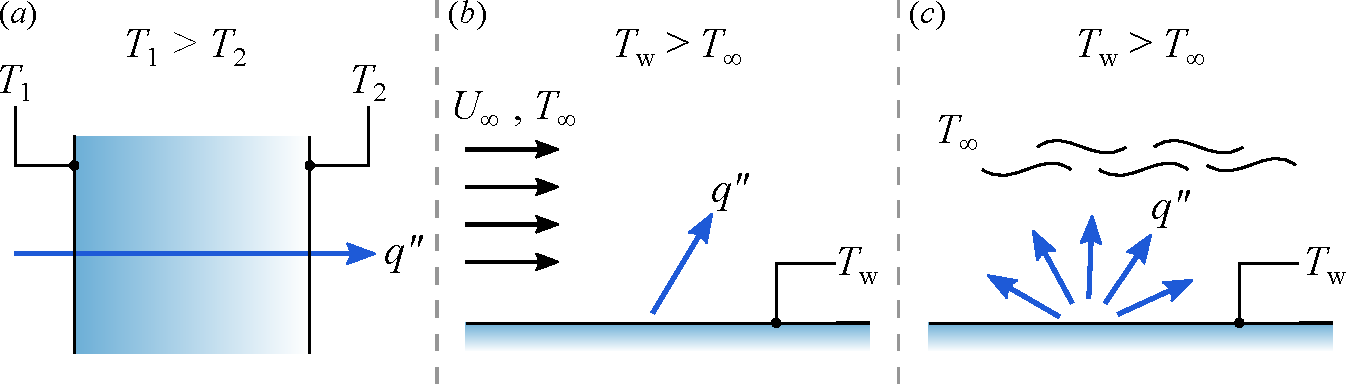
\includegraphics[width = 0.8\linewidth]{figures/dibujo_heat.pdf}
    \caption{Heat transfer mechanisms. (a) Conduction through a solid or a stationary fluid, (b) Convection from a wall to a moving fluid, (c) Radiation from a wall to the surrounding space. Figure adapted from \citet{bergman2011fundamentals}.}
    \label{fig:HTmethods}
\end{figure}

% Convection: the most complex
\citet{Gebhart1971HT} explains that the only physical mechanisms by which heat is transferred through and by the matter are conduction and radiation. However, if conditions occur in a moving medium, as is the case of fluids, the diffusion of thermal energy does not only happen at a microscopic level by the exchange of internal energy among molecules but also by the macroscopic motion of the moving medium. Eventually, this complex process is referred to as convection. Necessarily, convection becomes an additional heat transfer process to explain thermal energy transport in fluid flows. The study of convection includes all the mechanisms of conduction and radiation as well as those of the motion of fluids. Consequently, convection becomes the most challenging of the modes of transport within the field of heat transfer.

% Importance of heat transfer
Heat transfer gathers principles from thermal diffusion, electromagnetic radiation and fluid motion, including theories and knowledge from other branches of science. The study of heat transfer requires the mastery of many concepts and methods of analysis in several disciplines, with a crucial role in countless natural and industrial processes. The impact of thermal energy management on the current socio-economic environment is already discussed in Chapter~\ref{ch01}. Nonetheless, this is not a recent concern of modern science and engineering. In his communication to the Royal Society in 1852 (header of this chapter), Lord Kelvin concludes that there is a universal tendency in nature to the dissipation of mechanical energy, heat transfer being the mechanism driving this process. However, Lord Kelvin did not yet consider the dissipation of energy by convective heat transfer. 

%--------------------------------------------------------------------------------------------------
\subsubsection*{Heat transfer in fluid flows: Convection}

Convection is the heat transfer method of fluids par excellence. Depending on the nature of the fluid motion, convection may be classified into two different types. On the one hand, \textit{forced convection} occurs when the fluid motion is induced by external sources, such as a pump, a blower or the atmospheric wind. Forced convection is the predominant kind in both natural and industrial processes, as is the case of wall-bounded flows, jet shear layers or atmospheric flows. On the other hand, \textit{natural convection} happens when the motion is a direct consequence of buoyancy effects due to the temperature-induced density change within the fluid. A classic example of natural convection is the so-called Rayleigh–Bénard convection \citep{Bodenschatz2000RBC}.
%As an example, \citet{sanmiguelvila2016hconv} studied the onset of horizontal convection experimentally by differential heating on the bottom wall of an encapsulated fluid, and \citet{Shishkina2011Rayleight} applied model-free control strategies to control RBC in a two-dimensional domain. 
% From a flow-control standpoint,

This work focuses on the forced convection in wall-bounded flows, in which the mainstream exchanges energy with the wall surface, as depicted in figure~\ref{fig:dibujo_ThBL}. Two essential concepts are to be introduced, namely the boundary layer and turbulence. As defined in Chapter~\ref{ch01} and expanded in Chapter~\ref{ch04}, turbulence is a flow regime characterised by its nonlinear, chaotic and high-dimensional nature. Additionally, the \textit{boundary-layer} (BL) concept is the baseline of modern fluid mechanics, developed by Ludwig Prandtl in 1904 \citep{prandtl1904BL}. Upon the motion of fluid over a solid surface, a thin layer of air develops at the interface in which the fluid adjusts its velocity from that of the free stream to that of the solid. This region is characterised by strong velocity gradients along the wall-normal direction; hence, viscous effects dominate the flow. This region is commonly known as hydrodynamic, or velocity, boundary layer, and its thickness is denoted by $\delta$. 
Similarly, for incompressible flows, the thermal BL develops when the wall temperature $T_\mathrm{w}$ differs from that of the free stream $T_\infty$, inducing a temperature gradient normal to the wall. The development of velocity and thermal boundary layers is driven by momentum and thermal diffusivity, which are related by a dimensionless group named the Prandtl number ($\nPr$), which relates the kinematic viscosity $\nu$ and the thermal diffusivity $\alpha$ as
\begin{equation}
    Pr = \frac{\text{Momentum diffusivity}}{\text{Thermal diffusivity}} = \frac{\nu}{\alpha}
\end{equation}

The Prandtl number can be used to determine the relation between velocity and thermal BL thicknesses ($\delta$ and $\delta_t$, respectively). As illustrated in figure~\ref{fig:dibujo_ThBL}, for $\nPr >1$, $\delta > \delta_t$, meaning that the flow is dominated by the diffusion of momentum whereas for $\nPr < 1$, the flow is dominated by thermal diffusion so that $\delta < \delta_t$.

\begin{figure}
    \centering
    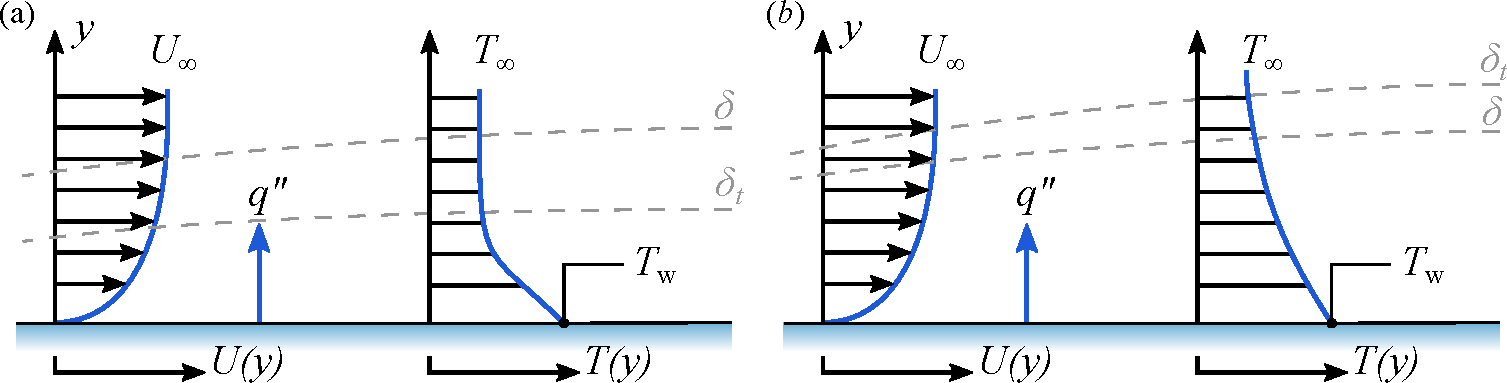
\includegraphics[width = 0.8\linewidth]{figures/dibujo_ThBL.pdf}
    \caption{Boundary layer development on a flat plate with convective heat transfer. (a) Thermal boundary layer thinner than the velocity boundary layer ($Pr > 1$); (b) Thermal boundary layer thicker than the velocity boundary layer ($Pr < 1$). The symbols correspond to wall-normal coordinate $y$, wall temperature $T_\mathrm{w}$, heat flux from the wall $q''$, and freestream velocity and temperature $U_\infty$,$T_\infty$, respectively.}
    \label{fig:dibujo_ThBL}
\end{figure}

Recalling the definition by \citet{Gebhart1971HT}, discussed above, convection is comprised of the energy dissipation due to random molecular motion and the bulk energy transfer due to the motion of the fluid at a macroscopic scale. These mechanisms are referred to as \textit{diffusion} and \textit{advection}, respectively. In turbulent boundary layers (TBLs), advection is dominated by the motion of coherent structures. From a thermodynamical perspective, coherent structures can be defined as fluid volumes moving collectively and with similar thermodynamic properties. The molecules composing the coherent structures retain their random motion through which diffusion is accomplished; hence the total thermal energy transport results from the superposition of random molecular motion on the microscopic scale and bulk fluid motion on the macroscopic scale. In other words, convective heat transfer is the cumulative effect of diffusion and advection. Diffusion is predominant in the near-wall region, where large eddies vanish into smaller scales dissipating energy. At the surface boundary, where the flow velocity adjusts to that of the wall, heat is transferred by diffusion only. The bulk energy transport is carried out by large structures within the boundary layer, exchanging heat with the free stream as well.

Regardless of the nature of the convection heat transfer process, the convective heat flux $q''~(\mathrm{W/m}^2)$ between the fluid and the boundary surface is determined from Newton's law of cooling, namely
\begin{equation}\label{eq:Newton_cooling}
    q'' = h(T_\mathrm{w} - T_{\mathrm{aw}})
\end{equation}
where the parameter $h~(\mathrm{W/m}^2\cdot\mathrm{K})$ is referred to as the convection heat transfer coefficient, and $T_{\mathrm{aw}}$ is the adiabatic wall temperature. The adiabatic wall temperature is a reference temperature of the fluid at which the heat transfer between the fluid and the wall is null. Its value depends on the flow conditions. For incompressible flows, as considered throughout this dissertation, the adiabatic wall temperature practically coincides with that of the undisturbed stream, i.e. $T_{\mathrm{aw}} \approx T_\infty$. Instead, for compressible flows, the reader is referred to \citet{Germain1955taw}, in which an extensive analysis and formulation are available.

Equating the heat conducted from the wall by the fluid by Fourier's law of thermal conductivity to the same heat transfer expressed in terms of a convection mechanism by Newton's law of cooling, the following relation is achieved:
\begin{equation}\label{eq:cond_conv}
    -k \left. \frac{\partial T}{\partial y} \right|_{y = 0} \equiv h(T_\mathrm{w}-T_\infty)
\end{equation}
where $k$ is the thermal conductivity of the fluid. The left-hand side in Eq.~\eqref{eq:cond_conv} represents the heat removed from the wall since no fluid flows through the wall. This relation can be expressed in dimensionless form as
\begin{equation}\label{eq:Nu}
    \left. \frac{\partial \left( \frac{T_\mathrm{w}-T}{T_\mathrm{w}-T_\infty}\right)}{\partial (y/\ell)} \right|_{y/\ell = 0} = \frac{h\ell}{k} \equiv \nNu_\ell.
\end{equation}
being $\ell$ a characteristic length of the flow under consideration, and $\nNu_\ell$ the Nusselt number based on $\ell$. The Nusselt number, as defined in Eq.~\eqref{eq:Nu}, may be interpreted as the ratio of heat transfer rate by convection to that of pure conduction through the medium. This dimensionless group is a classical form to refer to the convective heat transfer; however, it must not be mistaken with the Biot number ($\nBi = h\ell/k_\mathrm{w}$, being $k_\mathrm{w}$ the thermal conductivity of the solid wall), which is the ratio of the internal conductive resistance of a solid to the boundary layer convective resistance.

The study of convective heat transfer in fluid flows reduces to the determination of $h$. For experimental investigations, measuring heat fluxes at the wall requires both heat-flux sensors and temperature transducers. Papers 2, 3 and 5 in Part II of this manuscript, rely on the same methodology consisting of a heated-thin-foil sensor together with infrared thermography to acquire temperature. The heated-thin-foil is thermally thin \citep{astarita2012infrared}, i.e. it can be considered isothermal across its thickness since the Biot number is small for all the proposed problems ($\nBi < 0.1$). This non-intrusive measurement technique captures the distribution of convective heat flux on a surface. The interested reader is referred to the methodology section of Papers 2, 3 and 5 in Part II. 
%the Fourier number ($\nFo = \alpha_{s}/fs_{s}^2$, where $\alpha_{s}$ is the thermal diffusivity of the sensor, $s_{s}$ is the sensor thickness and $f$ is the IR camera sampling frequency, much larger than the inverse of the time scale of the phenomenon) is larger than unity; consequently, according to [20] the temperature distribution along the thickness of the printed circuit board is linear.
%-----------------------------------------------------------------------------------------
\subsubsection*{Analogy between Momentum and Heat Transfer}

The transport of momentum and energy in turbulent flows is based on similar mechanisms. The transport equations of these two quantities resemble each other. In their dimensionless form, the equations are analogous, depending on a few parameters, namely the Reynolds number \nRe, the Prandtl number \nPr, and the Nusselt number \nNu~(or the Stanton number \nSt, later introduced). There exist several versions of the momentum and heat transfer analogy. The most relevant are briefly described below, avoiding the mathematical process to obtain them for brevity. The interested reader is referred to the wide variety of textbooks on heat and mass transfer that cope with this topic \citep[\eg][]{bergman2011fundamentals,Lienhard2020}.

The first attempt to formulate this similarity was the famous Reynolds analogy. \citet{reynolds1874analogy} suggested that the concentration, velocity and temperature distributions should have a similar form, proposing a simplified mathematical rule that relates momentum and heat transfer processes.
\begin{equation}\label{eq:Re_analogy_aux}
    \frac{h}{\rho U_\infty c_p} = \frac{1}{2}\frac{\tau_w}{1/2\rho U_\infty^2}
\end{equation}

The right-hand side in Eq.\eqref{eq:Re_analogy_aux} represents the dimensionless representation of the wall shear stress $\tau_w$ (the Fanning friction factor $f = 2\tau_w / \rho U_\infty^2$), whereas the left-hand side of Eq.\eqref{eq:Re_analogy_aux} is a dimensionless group referred to as the Stanton number (\nSt) that measures the ratio of heat transferred to the fluid ($h$) to the fluid thermal capacity ($\rho U_\infty c_p$ being $\rho$ the fluid density, $U_\infty$ its velocity, and $c_p$ its isobaric specific heat). In other words, \nSt~describes the relationship between the heat transfer and the shear force at the wall, which translates into a geometric similarity between the velocity boundary layer and the thermal boundary layer. Hence, the Stanton number directly refers to $\nNu$, $\nPr$ and $\nRe$, relating momentum and thermal processes. The definition and physical interpretation of the Stanton number reads
\begin{equation} \label{eq:Stanton}
    \nSt = \frac{\text{Actual heat flux to the fluid}}{\text{Maximum possible enthalpy change}} = \frac{h\cancel{\Delta T}}{\rho U_\infty c_p\cancel{\Delta T}} = \frac{\nNu}{\nPr\nRe}
\end{equation}

Developing Eq.\eqref{eq:Re_analogy_aux}, Reynolds' analogy in its classical form reads as
\begin{equation}\label{eq:Re_analogy}
    \nSt = \frac{f}{2} \qquad \text{Reynolds analogy \citep{reynolds1874analogy}}
\end{equation}

Similarly, \citet{prandtl1910beziehung}, unaware of the pioneering work by \citet{reynolds1874analogy}, pointed out that the velocity and temperature differential equations are identical when the thermal and momentum diffusivities are equal. Both Reynolds' and Prandtl's analogies are valid for the simplified case of a boundary layer that develops on a flat plate under zero-pressure-gradient (ZPG) conditions and in the limit of $\nPr = 1$. Soon an unsuccessful attempt by \citet{taylor1916conditions} tried to formulate a generalized analogy for cases with $\nPr \neq 1$. \citet{colburn1933analogy} explored the relevance of the Prandtl number on the turbulent transport similarity. By combining energy and momentum transport equations within a turbulent boundary layer on a flat plate, the group $\nSt\nPr^{2/3}$ arises, which is defined as the $j$-factor. This analogy is an extension of classical Reynold's analogy, which is commonly known as the $j$-factor or Chilton-Colburn analogy \citep{Chilton1934Jfactor},
\begin{equation}\label{q:jfacto_analogy}
    \frac{f}{2} = j = \nSt\nPr^{2/3} = \frac{\nNu}{\nRe\nPr^{1/3}}
\end{equation}

The validity of these analogies is nonetheless restricted only to the boundary layer flow on a flat plate under ZPG conditions. Several authors aimed at developing more general models to relate heat and momentum transport; however, most of them rely on empirical coefficients or are case-dependent. For the reader's interest, an extensive review of heat-momentum analogies is presented by \citet{churchill1997critique}. %The above discussion is intended to present to the reader the concept of the heat and momentum transfer analogy, the principle of similarity between these two mechanisms and the definition of the Stanton number. Understanding these concepts enables exploring solutions for heat transfer control in other fields such as skin-fiction reduction, mixing enhancement or wake suppression. Furthermore, Paper 1 in Part II of this thesis leverages the Reynolds analogy to investigate an approach to reducing heat transfer in turbulent boundary layers.

%================================================================================================
%- Heat transfer control:
%================================================================================================
\section{Strategies for heat transfer control}

Heat transfer control is the discipline that explores thermal management strategies with the target of altering the mechanisms behind thermal energy transport. This discipline is commonly known as \textit{heat transfer enhancement} since most efforts are aimed at increasing the heat transfer capabilities of the system. Heat transfer enhancement is present in many industrial and research areas, such as space satellites' thermal management by radiation, conduction mechanisms in solar panels or convective heat fluxes in heat exchangers of engines. In this section, the focus lies on convective heat transfer control, performance quantification criteria, and the strategies to achieve enhancement. 

For an enhanced surface in single-phase flows, the ``basic performance characteristic'' is the $j-$factor from the Chilton-Colburn analogy, together with the friction factor, $f$, as a function of the Reynold number, $\nRe$. A straightforward possibility to quantify the performance enhancement is to calculate the ratios $j/j_0$ and $f/f_0$, where the subscript $0$ is for the reference condition. Although it depends on the enhancement strategy in use, commonly $f > f_0$ under the same $\nRe$. Thus, this approach does not accurately quantify the actual performance improvement, subject to specific operating constraints. Considering $j/j_0$ may yield unfair comparisons since the enhanced flow condition is allowed to operate at a higher pressure drop than the reference. In other words, the reference flow condition could achieve higher $h$ if operated at higher $\nRe$ to balance the pressure drop to that of the enhanced case. Therefore, the additional energy required to promote the enhanced heat transfer condition must be quantified to determine the performance fairly.

In the literature, there exist several measures of \textit{performance} for heat transfer enhancement strategies. It is worth noting that heat transfer enhancement is a discipline strongly related to the design, study and optimisation of heat exchangers. Based on the discussion by \citet{manglik2003heat}, the performance evaluation criteria (PEC) for single-phase flows strongly depend on the objective of the enhancement. A general formulation is proposed by both \citet{manglik2003heat} and \citet{webb2005enhanced} that relates the change in heat transfer coefficient $h$ for a heat transfer surface $A$ with the required pumping power $P$. This classical interpretation for heat transfer enhancement reads,
\begin{equation}\label{eq:PEC}
    \frac{hA/h_{0} A_{0}}{(P/P_{0})^{1/3}(A/A_{0})^{2/3}} = \frac{j/j_{0}}{(f/f_{0})^{1/3}},
\end{equation}
The general PEC is driven by the three variables on the left-hand side, namely ($hA/h_0A_0$), ($P/P_0$), and ($A/A_0$). By setting one of the variables as the objective, the remaining two are considered operating constraints, fixing their values to 1.0. In this work, the PEC in Eq.~\eqref{eq:PEC} is adjusted to the case of a turbulent boundary layer flow in which the thermal energy transfer process is mainly driven by a change in temperature between the mainstream and the wall. Consequently, the heating/cooling area and the Reynolds number are unaltered when applying the heat transfer enhancement technique, $A/A_0 = 1$. Therefore, the main objective of the herein considered problems is to control the value of $h$, while the power requirement is envisioned as a penalty term in the objective function. A deeper discussion on the formulation of the optimisation problem is provided in Chapter~\ref{ch03}.

The heat transfer control problem is then classified into different categories, depending on whether the objective is to enhance or reduce heat transfer and on the type of control strategy in use. For the latter, literature differentiates between \textit{passive} and \textit{active} techniques \citep[\eg][]{webb2005enhanced}. Passive flow control techniques are those that perform the actuation regardless of an external power supply. This is commonly achieved by geometry alteration of the surface such as roughness elements \citep{Hwang1995roughness,Hechuan2018ratchet}, obstacles \citep{mallor2018cubes}, riblets \citep{Mallor2019ribPOD}, or vortex generators \citep{Awais2018review,Ke2019VG}. Despite the undoubted effectiveness of passive elements, these devices are constantly present in the flow field, inducing a continuous pressure drop that translates into an undesired skin-friction augmentation. The inability to trigger the control action when desired or to adjust the control authority also deteriorates the performance of passive elements. Active control techniques cope with all the enumerated weaknesses at the cost of an external power supply to perform the actuation on the flow. There are countless active flow control devices such as continuous \citep{puzu2019jet} or synthetic \citep{Giachetti2018synjet} jets in crossflow, plasma actuators \citep{roy2008plasma}, electromagnetic forcing \citep{Kenjere2008EMheat} or moving walls by electroactive materials \citep{Leal2013rev_electroactive}, to name a few. Active control has gained interest in the flow control and heat transfer communities during the last decades due to its outstanding versatility in the control design, from the actuator to its control logic. Furthermore, the incursion of sophisticated algorithms into flow control triggers the possibility of exploring unconventional flow control strategies, adjusting their authority upon the requirements of the flow according to a pre-stated objective.

In this work, the focus lies on a specific mechanism through which heat transfer enhancement is achieved in turbulent flows, which consists of inducing streamwise vortices embedded in the boundary layer \citep{jacobi1995}. The resulting near-wall coherent structures prevail over a significant downstream distance, promoting cross-stream momentum transfer within the boundary layer. This actuation facilitates the transport of high-momentum fluid from the outer region towards the wall, exacerbating heat transfer and turbulent mixing. Classical, passive heat transfer enhancement methods exploiting this principle are wall-mounted obstacles and vortex generators. 
%For the latter, there are three basic recommendations to design the VG: longitudinal vortices are more effective than transversal vortices; (2) delta winglets outperform rectangular winglets; and (3) optimum angles of attack lies in the range $[30^\circ,45^\circ]$.
Vortex generators (VG) are widely used in the aeronautical industry as a passive element to promote turbulence transition on adverse-pressure gradient flows \citep{Lin2002reviewVG} and in heat transfer enhancement applications such as heat exchangers \citep{Awais2018review}.  Regarding wall-mounted obstacles, the work by \citet{Chyu1996obstacles} investigates the flow topology and heat transfer distribution around several obstacle shapes. A horseshoe vortex develops upstream with the corresponding streamwise counter-rotating vortex pair extending downstream at both sides. At the downstream side of the obstacle, the flow separates and recirculates, yielding a reduction of convective heat transfer at the wall. The flow re-attaches further downstream with an impinging flow known as the arch-shaped vortex. According to \citet{Chyu1996obstacles}, the cubes are the best shape for heat transfer enhancement purposes upstream of the obstacle. However, they present a strong recirculation area as demonstrated by \citet{nakamura2001cube}. \citet{mallor2018cubes} aimed to solve this issue by perforating the wall-mounted cubes similar to the perforated fins in channel flow used by \citet{Hwang1995roughness}. Perforated cubes not only reduce the recirculation region but also increase the maximum Nusselt number at the wall due to the impingement of the flow coming through the perforation. It is worth noting that the flow around an obstacle resembles that induced by other active elements as the jets in cross flow \citep{fric_roshko_1994}. A detailed description of jets in cross flow reads in section~\ref{ss:JICF}.

On the contrary, few contributions exist regarding heat transfer reduction in turbulent boundary layers. The early and extensive study by \citet{Moffat1984review} investigates a TBL when submitted to different perturbations such as acceleration, deceleration, roughness and surface curvature, among others. Although this study may seem obsolete, it pointed out several basic flow mechanisms to modify the Stanton number that have been later better explained and exploited for flow control, such as the opposition control \citep{Choi1994}. In that respect, the contributions in skin-friction drag reduction are counted by hundreds, which could be extrapolated to convective heat transfer reduction by invoking the analogy between momentum and heat transfer described above. Most effective flow control techniques to reduce momentum flux must interrupt the bursting cycle's self-sustaining regenerative process \citep{hamilton1995,Jimenez1999,schoppa2002}. Typically, the cycle envisions the generation of low-speed streaks by the lift-up effect of fast-advecting streamwise vortices \citep{Butler1993streak} within the boundary layer. Then, the transient growth of the streaks collapses in the regeneration of streamwise vortices \citep{hamilton1995,schoppa2002}. The so-called opposition control \citep[\eg][]{Choi1994,Stroh2015,Fukagata2003oppcontrol} is the most classical approach used to reduce skin-friction drag, which aims at damping coherent structures in the near-wall region. Another classical approach is the generation of embedded streamwise vortices within the turbulent boundary layer, as proposed by \citet{Schoppa1998}. A 20\% drag reduction in a turbulent channel upon generating large-scale counter-rotating streamwise vortices by wall jets. In contradiction to the above discussion for heat transfer enhancement, the large-scale swirl motion merges streaks into a larger streak envelope with reduced strength, thus cancelling the generation of streamwise vortices in the last part of the bursting cycle and reducing drag \citep{schoppa2002}. The heat transfer footprint of streamwise vortices embedded in a TBL is investigated by \citet{Zhang1993heatJICF}, concluding that those vortices that are deeply embedded with a reduced size and strength are the ones that could be used to reduce heat transfer and skin friction. Similar experimental investigations use jets vortex generators \citep{iuso2002} or body forces by plasma actuators \citep{cheng_wong_hussain_schroder_zhou_2021} to induce large-scale vortical motion that effectively reduces skin-friction drag.\\

The following sections provide a detailed description of the active flow control techniques used in this thesis. Plasma actuators are employed in Paper 2 to reduce heat transfer whereas jets in cross flow are tuned in Papers 3 and 5 to maximise the convective heat transfer.

%------------------------------------------------------------------------------------------
\subsection{Plasma actuators}\label{ss:PA}

The term \textit{Plasma} was first coined by \citet{Langmuir1928plasma} to denote an electrically-neutral ionised gas. Since then, the term plasma has been used in physics to define when substances feature charge equilibrium, generally known as the \textit{fourth state of matter}. Hence, plasma is a gaseous system of free-floating charged species that mutually interact, providing outstanding electromagnetic response of the plasma cloud and good electrical conductivity. The study of plasma and its applications have received overwhelming attention in the past, especially in flow control, space propulsion, material science and medicine, among others. The interested reader is referred to the extensive work by \citet{fridman2008plasma} to delve into plasma physics.

The production and preservation of a plasma discharge come hand in hand with several technological challenges due to the considerable energy requirement for promoting gas ionisation and the degradation of materials nearby the plasma cloud. The ionisation of a given volume of gas is usually achieved by applying an electric field, which is generated by either direct current (DC) or alternating current (AC) voltage. There is a minimum required voltage to sustain electron-ion pairs in the gas, the \textit{breakdown voltage} $E_b$, which depends on several factors like the driving frequency, the temperature and pressure of the gas, or the chemical composition of the gas \citep{Kunhardt1980breakdown,kunhardt1983electrical}. For the particular case at standard atmospheric conditions using air as a gas, the produced plasma is characterised by incomplete ionisation and no thermal equilibrium. Hence, the energy provided by the electric field is mainly stored in the free electrons, which translates into a relatively low temperature, given the name of \textit{cold plasma} \citep{Yamamoto2007plasma}. This kind of plasma is typically used in flow control applications as later proposed in this thesis.

The plasma actuators are devices that generate plasma to induce body forces in a specific manner. According to the extensive review by \citet{Kotsonis2015review}, plasma actuators are the modern technological implementation of Aristotle's concept of the \textit{unmoved mover}. The plasma actuator is a static device that can induce motion in the surrounding fluid without moving parts or the injection of a secondary stream. There are several alternatives for plasma actuators such as alternating current dielectric barrier discharge (AC-DBD) \citep{Roth1998dbd}, direct current corona (DC-corona) \citep{Leger2001corona}, nanosecond pulsed dielectric barrier discharge (ns-DBD) \citep{Roupassov2009nsplasma}, and arc filament actuators \citep{Samimy2004arcfilament}. In the following, only AC-DBD plasma actuators are considered, which is the kind used in this thesis.

\begin{figure}
    \centering
    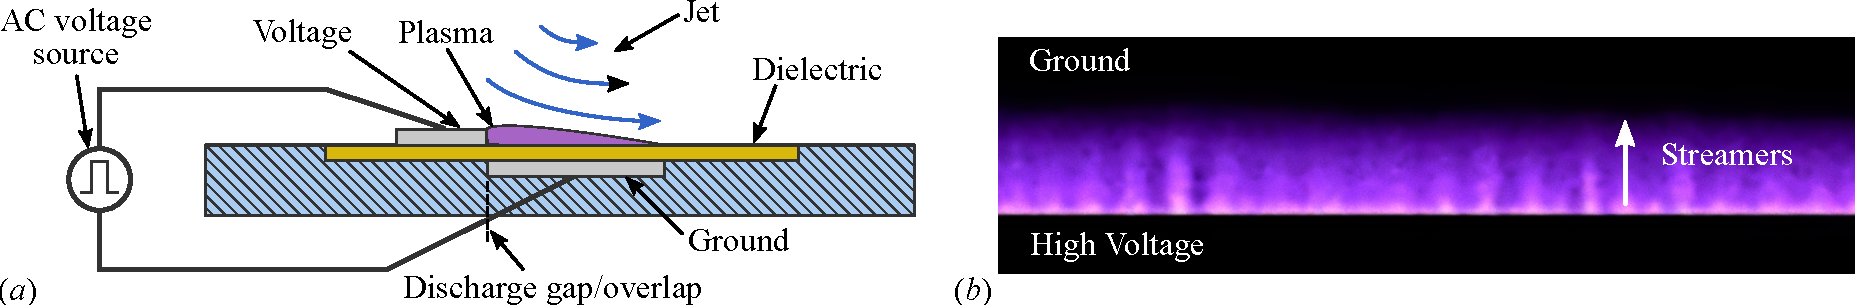
\includegraphics[width = 0.99\linewidth]{figures/schematic_plasma.pdf}
    \caption{AC-DBD plasma actuator. (a) Schematic of a typical cross-section of an asymmetric AC-DBD plasma actuator. (b) Top-view photograph of the purple glow on a DBD plasma actuator.}
    \label{fig:schematic_plasma}
\end{figure}

The specific dielectric-barrier-discharge configuration consists of two electrodes separated by a dielectric material. One of the electrodes is referred to as \textit{encapsulated}, which is commonly grounded and covered by the dielectric material. The remaining electrode is known as \textit{exposed}, since it is in direct contact with the surrounding fluid. The latter is connected to a high-voltage supply that is used to reach the breakdown voltage to generate plasma. Note, however that the opposite configuration with a high-voltage \textit{encapsulated} electrode and a grounded \textit{exposed} electrode is also possible. For a single plasma actuator configuration in which only one plasma plume is produced, the electrodes arrange as shown in figure~\ref{fig:schematic_plasma}(a). Upon the application of high voltage (HV), charge tends to accumulate on the surface of the dielectric material, yielding filamentary micro discharges, also known as streamers \citep{Kogelschatz2002filamentary} (figure~\ref{fig:schematic_plasma},b). These streamers change the capacitance of the dielectric barrier, reversing the local electric field and, thus, terminating themselves \citep{Eliasson1991streamers}. Based on this phenomenon, a continuous plasma discharge requires the application of variable voltage, either in the alternating or pulsating form \citep{michelis2017boundary}. Although the application of DC voltage is possible by substituting the dielectric barrier with a resistive barrier \citep{Laroussi2002resistive}, the most typical configuration of DBD actuators employs AC voltage, as shown in figure~\ref{fig:schematic_plasma}. For an AC-DBD plasma actuator working in air, the plasma is characterised by the back-and-forth motion of heavy ions, following the AC polarity inversion. This motion promotes collisions among the heavy-charged species (positive and negative ions), which results in a momentum exchange with the surrounding air \citep{Kotsonis2015review}. The resultant electric field and, thus, discharge are asymmetric due to the electrode arrangement. Consequently, the momentum exchange produces an uneven body force that directs from the exposed to the covered electrode, which induces a wall-tangent motion of the fluid. The resultant wall-jet structure, also referred to as \textit{ionic wind} \citep{Benard2014review}, injects fluid at a velocity which does not typically exceed $10\mathrm{m/s}$ \citep{Moreau2007review}.

Flow control strategies based on plasma actuators received much interest during the last few decades, still being very promising due to their electric nature. As the Aristotelian \textit{unmoved mover}, plasma actuators do not need movable parts to induce a fluid motion. At the same time, these devices feature a high-frequency response, being fully controllable in terms of amplitude and frequency within their operating limits. From a practical standpoint, plasma actuators require low power to operate, and their manufacturing is rather simple. In addition, they are very versatile in terms of geometrical patterns, extension, and thickness, which makes them very suitable to be flush-mounted devices with minimal flow disturbance while inducing body forces in the desired region direction and shape. Besides their control authority restricting their application to high Reynolds numbers, the aforementioned factors make DBD plasma actuators good choices for controlling aerodynamic flows such as laminar-to-turbulent transition \citep{Grundmann2008cancelTS,kotsonis2015control} and separation \citep{Little2010airfoilplasma,Michelis2015track}. A thorough summary of flow control studies based on DBD-plasma actuators is provided by the extensive reviews by \citet{Moreau2007review}, \citet{Corke2010}, \citet{Benard2014review}, and \citet{Kotsonis2015review}.

Plasma actuators have also been used to control the momentum fluxes within turbulent flows, especially for skin-friction reduction. A common approach consists of inducing spanwise travelling waves or spanwise oscillations. This strategy relies on the classic drag-reduction methodology proposed by \citet{Schoppa1998}, which aims at generating streamwise vortices embedded in a boundary layer to reduce momentum fluxes at the wall. In this regard, the experimental study of \citet{Whalley2014} employs a set of different plasma actuators to investigate the effect of co- and counter-rotating streamwise vortices in a turbulent boundary layer. They conclude that the formation of the spanwise travelling wave enables the formation of wide ribbons of low-speed streamwise velocity within the viscous sublayer, which locally reduces skin friction. Likewise, \citet{jukes2006TBLcontrol} achieved a strong skin-friction drag reduction downstream of the plasma actuator. These so-called ``plasma streamwise vortex generators'' (PSVGs) consist of a single or an array of plasma actuators aligned with the flow direction. Hence, the momentum injection by the actuators is normal to the mainstream, which leads to twisting and folding of the flow that eventually transforms into a streamwise vortex \citep{jukes2013plasmaVG}. The use of streamwise-aligned plasma actuators has been investigated in laminar \citep[e.g.,][]{jukes2013plasmaVG,serpieri2017} and turbulent boundary layers \citep[e.g.,][]{Jukes2006, Whalley2010DBDvortex, Wittig2019VGplasma} with promising results as a skin-friction drag reduction technique. 

Regarding heat transfer control, DBD plasma actuator applications are rather unexplored. It is worth noting that, despite the non-thermal nature of cold plasma, the plasma discharge locally produces thermal energy that may lead to a thermal footprint. Nonetheless, most of the produced heat diffuses through the dielectric and is not released to the fluid flow \citep{Rodrigues2018,Jukes2006}. The DBD plasma actuator proposed in this thesis resembles to that studied by \citet{Whalley2014}, \citet{Wittig2019VGplasma}, and, especially, \citet{cheng_wong_hussain_schroder_zhou_2021} (see figure~\ref{fig:dbd_actuator}). According to \citet{Wicks2015}, for opposing plasma discharges, streamwise vorticity generates upon the re-orientation of wall-normal vorticity from the actuators and spanwise vorticity from the boundary-layer, towards the streamwise direction. The reason behind this choice is that, contrary to conventional spanwise-aligned actuators, injecting momentum in the free stream direction to energise or weaken the boundary layer, the generation of streamwise vortices could potentially reduce turbulent fluxes at the wall. The research in Paper 2 thus aims at reducing convective heat transfer with an array of plasma actuators streamwise vortex generators. 

\begin{figure}
    \centering
    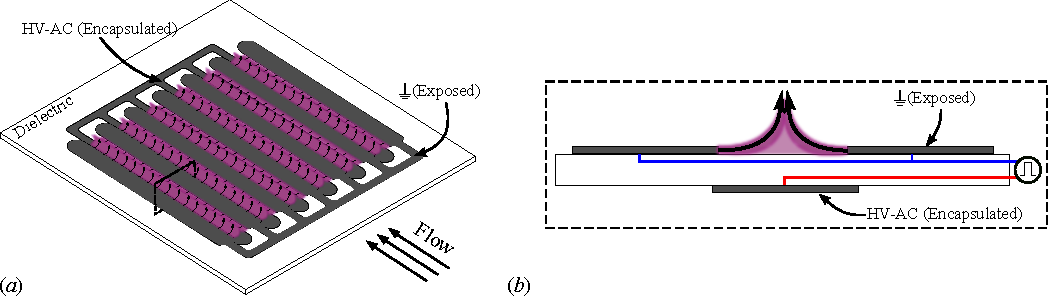
\includegraphics[width = 0.99\linewidth]{figures/dbd_actuator.pdf}
    \caption{Schematic representation of the DBD-plasma actuator array used in Paper 2. (a) Tri-dimensional representation of the array, and (b) cross-section of a pair of actuators.}
    \label{fig:dbd_actuator}
\end{figure}

As shown in figure~\ref{fig:dbd_actuator}, an array of DBD plasma actuators is considered in this thesis. Each actuator shares the encapsulated electrode with its adjacent. A total of 6 linear bi-directional actuators is used to ensure spanwise uniformity of the plasma-induced control. In this particular case, the air-exposed electrode is grounded while the encapsulated electrode beneath the dielectric material is connected to a stable high-voltage supply. As described in Paper 2 of this thesis, the actuator generates a sequence of opposing wall jets tangent to the surface in the spanwise direction, inducing pairs of counter-rotating streamwise vortices. In the recent study by \citet{cheng_wong_hussain_schroder_zhou_2021}, pairs of streamwise counter-rotating vortices are induced by plasma, merging with natural TBL streaks and interrupting the turbulence regeneration cycle, thus reducing skin friction. Invoking Reynolds' analogy of momentum and energy fluxes in turbulent boundary layers, the methodology proposed in Paper 2 exploits the same principles for an effective reduction of convective heat transfer in a turbulent boundary layer.

%------------------------------------------------------------------------------------------
\subsection{Jets in crossflow}\label{ss:JICF}

The jet in crossflow (JICF), or transverse jet, is a complex flow configuration present far and wide in natural processes and engineering applications. It is possible to find JICF in natural phenomena such as volcanic eruptions or the merge of a river and its tributary, although they are most commonly studied due to their relevance in the engineering field like for film cooling of turbine blades or thrust vector control for missiles, to name a few. Thus, the jet in crossflow can be adapted to the application, with several possible alternatives in nozzle size and shape, pulsation, inclination of the injection plane or injected fluid, for instance. The extensive field of application and variations of JICF requires a deep understanding of the flow topology, mixing, structural and sometimes reactive features to accurately design the operating and control conditions \citep{Karagozian2014revJICF}.

The utilisation of transverse jets for flow control is still an active research field with constant technological development and practical applications. It is well-agreed that a jet stream interacting with a crossflow provides better mixing capabilities than a free jet or a mixing layer \citep{kamotani1972experiments, broadwell1984structure}. The complex interaction of the jet flow with the freestream induces a web of flow structures and vortex systems that must be properly understood and managed for an effective flow-control purpose. The canonical configuration of a steady round jet perpendicular to a crossflow has been widely studied in the last decades \citep{kamotani1972experiments, fric_roshko_1994, kelso1996experimental, broadwell1984structure, smith1998mixing} due to its relevance in several engineering fields, especially in air-breathing engines. 

Following the seminal research work by \citet{fric_roshko_1994} and the extensive reviews by \citet{Mahesh2013revJICF} and \citet{Karagozian2014revJICF}, four main vortical structures are distinguished, as illustrated in figure~\ref{fig:JICF}. Upon the interaction of the freestream flow with the jet stream, small coherent structures develop in the form of ring-like vortices, commonly known as shear-layer vortices, which dominate the upstream formation of the jet column and are found to have the same direction of vorticity and similar length scales as the boundary layer formed inside the jet. These vortical structures are said to be formed from instabilities in the jet's shear layer, particularly on Kelvin-Helmholtz instabilities near the jet exit \citep{fric_roshko_1994, kelso1996experimental}. It is worth noting that the jet shear-layer instability found on free and transverse jets are significantly different in nature and formation characteristics \citep{megerian2007transverse}. Second, dominating the jet cross-section, a counter-rotating vortex pair (CVP) is produced in the near-field region of the jet \citep{kamotani1972experiments}. This large vortical structure is responsible for the pressure difference between the downstream and upstream sides of the jet exit and the vorticity evolution in the shear layer of the jet stream \citep{andreopoulos1984experimental, cortelezzi2001formation}. The formation of the CVP is attributed to the roll-up of vortex rings in the near-field region of the flow. The interaction among the vortex rings, as well as their roll-up and deformation, can be influenced by changes in flow conditions, such as the crossflow velocity, jet velocity and boundary layer thickness and have a significant impact on the entrainment of the crossflow into the near-field of the jet \citep{smith1998mixing,kamotani1972experiments,cortelezzi2001formation}. Third, a system of horseshoe vortices wraps around the jet base \citep{Krothapalli1990HSvort} due to the interaction between the mainstream boundary layer and the transverse flow exiting the jet \citep{kelso1995horseshoe}. These trailing vortices resemble those formed in flows around wall-mounted cylinders but can also oscillate and coalesce with other structures in the flow, leading to an unsteady regime under certain flow conditions \citep{kelso1995horseshoe}. Last, smaller-scale structures build up downstream of the jet column primarily attached to the wall and contain fluid of the wall boundary layer that entrains into the jet stream \citep{fric_roshko_1994}. The formation mechanism of the wake vortices is fundamentally different from those found in the flow around solid cylinders as the vortices are not shed directly from the jet but originate in the wall boundary layer. Periodic separation of the wall boundary layer caused by adverse pressure gradients induces an upward release of fluid and vorticity that generates column-like structures rising from the wall \citep{fric_roshko_1994}. These coherent structures contribute to the transverse jet's complex structure and mixing characteristics \citep{smith1998mixing}. The horseshoe vortex and the CVP, in particular, play a key role since they add to the mean flow while the wake and shear vortices mainly affect the fluctuating dynamics of the jet \citep{karagozian1986analytical}.

\begin{figure}
    \centering
    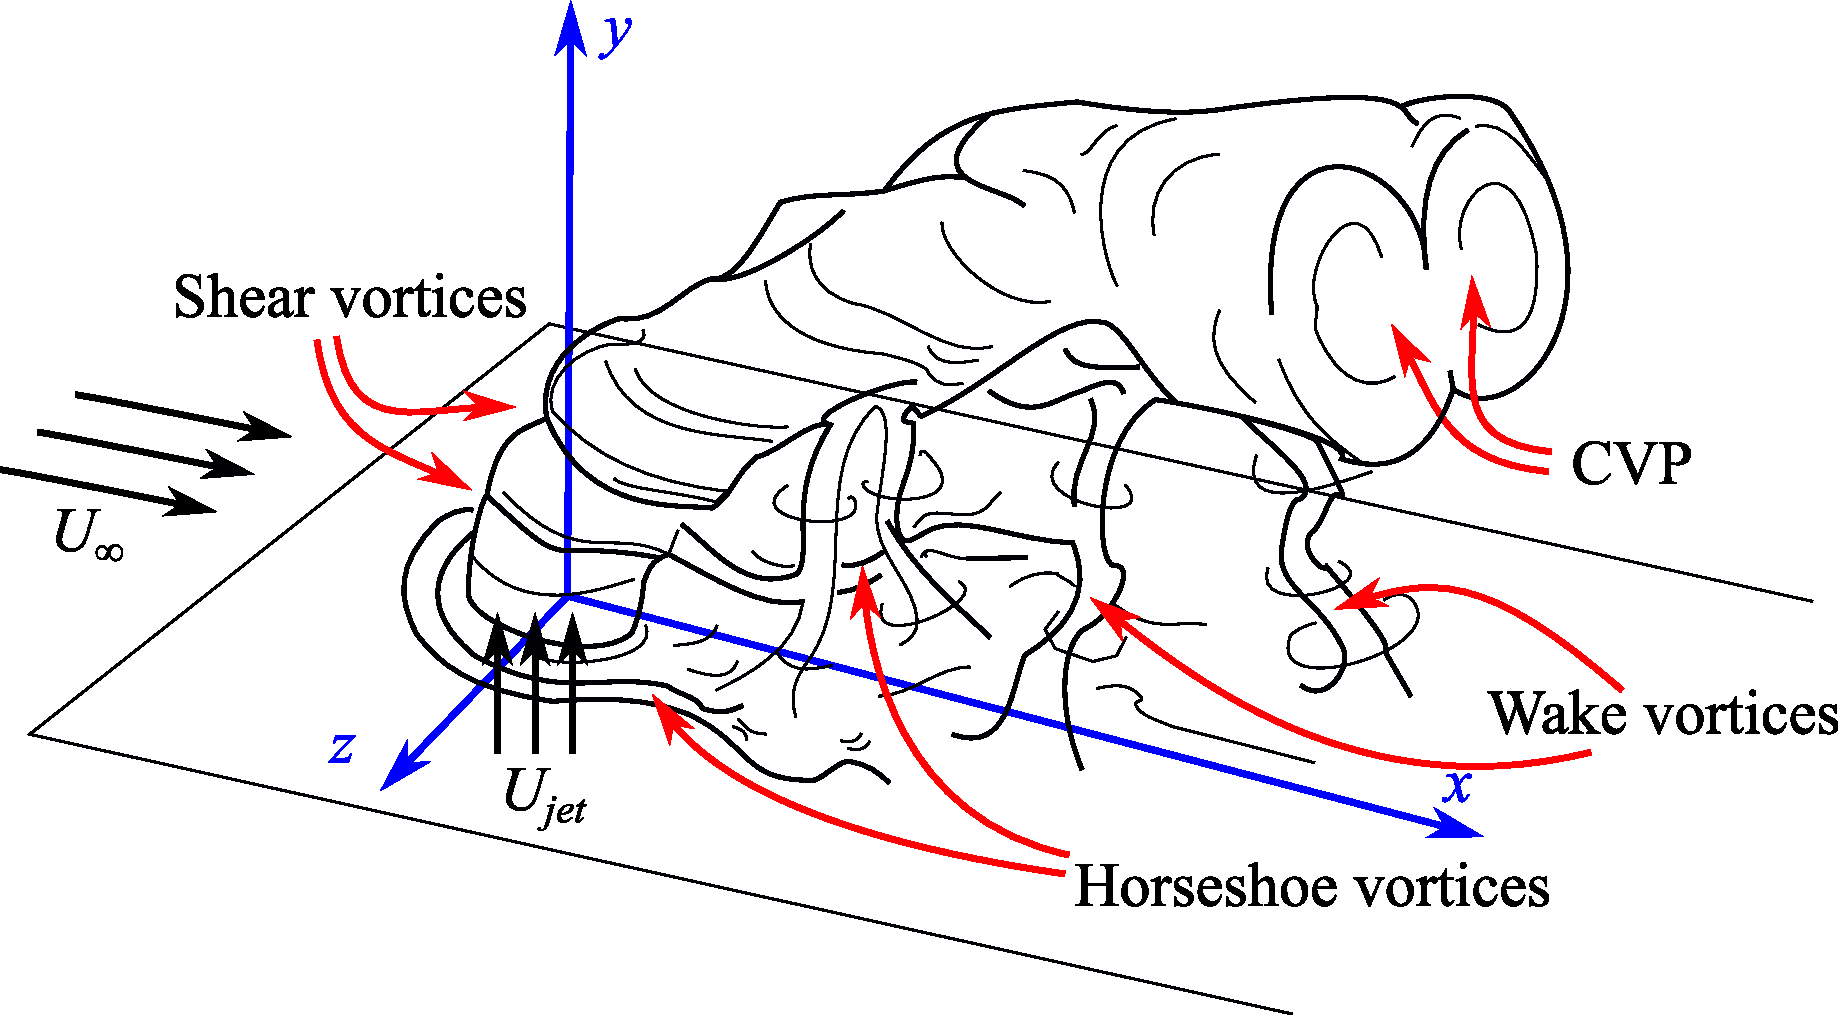
\includegraphics[width = 0.7\linewidth]{figures/JICF.pdf}
    \caption{Vortical structures for a round jet injecting steady fluid into a normal crossflow. Adapted from \citet{Karagozian2014revJICF}.}
    \label{fig:JICF}
\end{figure}

The mixing enhancement is the most common target when the JICF is used as a flow control actuator. This application is reported in the classic work by \citet{smith1998mixing}, which shows that the mixing enhancement narrows to the near-field region of the flow dominated by the CVP's structural formation and not to the far-field region where the CVP is fully developed. Regarding heat transfer enhancement applications, \citet{puzu2019jet} investigated the influence of the CVP and horseshoe vortices downstream of the jet injection. They report that the secondary mixing by the combined effect of the collapse of the CVP and the merge of the horseshoe vortices leads to a local convective heat transfer enhancement due to better entrainment and mixing within the boundary layer. Nonetheless, there is consensus that the pulsation or modulation of the JICF considerably improves its mixing performance compared to the steady jet. This matter is discussed in the experiments by \citet{vermeulen1992mixing, johari1999penetration, eroglu2001structure, MCLOSKEY2002, Johari2006scaling}, to name a few. \citet{vermeulen1992mixing} reported a considerable increase in the mixing area, penetration, and overall mixing by acoustically exciting a jet into a hot crossflow. They also concluded that the collapse of the structures and the interaction promoting mixing are displaced upstream, with higher mixing rates in the downstream vicinity of the injection. On the other hand, \citet{johari1999penetration} considered a fully-modulated JICF (valve-actuated) to study the effect of the frequency and duty cycle on the mixing properties, demonstrating that a short injection time (also referred to as pulse width) provides a higher mixing performance and dilution. The experiments by \citet{eroglu2001structure} and \citet{MCLOSKEY2002} focus on the induced perturbations on the vortical structures by the pulsation, finding that square-wave excitation generates distinct vortex rings. Most of the investigations of flow control with pulsed JICF agree on the importance of tuning the control strategy to find the optimal configuration that amplifies or optimises the desired flow feature \citep{shapiro2006optimization}. However, there is no universal objective function to drive the optimisation of pulsation due to the dependency on the flow and pulsation conditions, which are found to be apparatus-dependant \citep{MCLOSKEY2002}. The interested reader is referred to the extensive review article by \citet{karagozian2010transverse} covering the jet in crossflow and its control.

Besides the undeniable suitability of pulsed JICF for several flow control applications, there is still a profound lack of consensus on the flow structures, the dynamics and the correct scaling that characterise this flow configuration \citep{Sau2010optJICF}. The \textit{formation number} \citep{gharib1998scalingVR} is used in some studies \citep[e.g.][]{MCLOSKEY2002,shapiro2006optimization} to express the optimal pulsation condition, although this parameter was conceived for quiescent flows. \citet{Johari2006scaling} proposes the \textit{stroke ratio} and \textit{duty cycle} to scale the pulsed JICF together with a classification of induced structures such as hairpin vortices, vortex rings with or without trailing columns or turbulent puffs; nonetheless, \citet{Sau2008dynamicsVRICF} refuted this idea, demonstrating its validity just for quiescent flow conditions. The regime map suggested by \citet{Sau2010optJICF} builds upon two dimensionless parameters, namely the \textit{ring velocity ratio} and the \textit{stroke ratio}, gathering the effects of the pulsation frequency, duty cycle, modulation, and pulsed energy. For small ring velocity ratios, i.e. low injection velocities compared to the crossflow, the induced structures develop as hairpin vortices that progressively get closer as the stroke ratio is increased. There are two possibilities for high values of the ring velocity ratio: isolated vortex rings and vortex rings followed by a trailing column of vorticity, which depend on a low or high value of the stroke ratio, respectively. This map seems to reasonably fit with previous existing literature, showing that the optimal pulsation of JICF may be explained in terms of their vortex rings and that the optimal experimental conditions are seen to collapse on the same optimal curve. Howbeit, most of the engineering and technological studies that explore the utilization of pulsed JICF get behind the Strouhal number, $\mathrm{St}$, to characterise the modulation of the jet. In this regard, Paper 3 and Paper 5 of this thesis rely on the duty cycle and the Strouhal number as the scaling parameters to define the control action.

A simplified schematic of the pneumatic system used in Paper 3 and Paper 5 to generate the JICF is illustrated in figure~\ref{fig:schematic_pneumatic}. A pressurised air supply provides the jet stream. The air is filtered to avoid spurious oil or solid particles from entering the experimental setup. The control of the jet stream is performed in two steps. First, a pressure relief valve controls the absolute pressure on the system, which is always lower than that provided by the air compressor. This condition guarantees a constant operating pressure regardless of the jet actuation parameters. Second, a flowmeter and controller are used to monitor the flow condition, namely mass and volumetric flow rates, temperature, density and pressure. A settling chamber is used to prevent the flow meter and the pressure relief valve from spurious pressure waves induced by the ram effect at the solenoid valve. Eventually, a slot jet diffuser is used to progressively transition from a round shape of the pressurized line to the final rectangular shape at the jet exit.

\begin{figure}
    \centering
    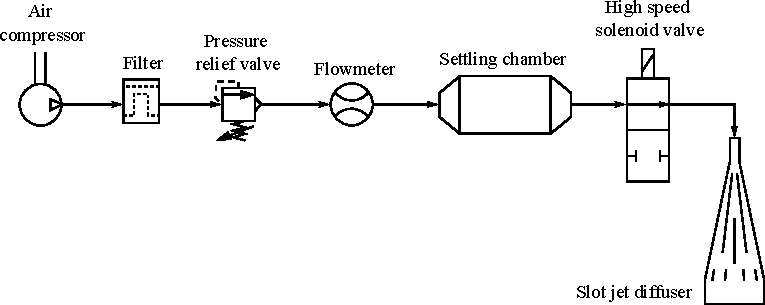
\includegraphics[width = 0.95\linewidth]{figures/schematic_pneumatic.pdf}
    \caption{Schematic of the experimental apparatus to control the jet in crossflow in the investigations of Paper 3 and Paper 5.}
    \label{fig:schematic_pneumatic}
\end{figure}

The dynamical behaviour and the flow topology of a non-circular JICF are very similar to those described above \citep{liscinsky1996crossflow, plesniak2005scalar}, especially in the far-field region of the flow. The interested reader is referred to the classic review by \citet{Gutmark1999noncirc}, where several investigations of flow control with non-circular jets are reported. In particular, the spanwise slot JICF has been investigated both experimentally and numerically for the steady-blowing configuration, and with jet modulation \citep[see e.g.][]{park1999, Krogstad2000slitjet, steinfurth2021CFslot}. The recent series of studies of pulsed slot jets in quiescent flow conditions \citep{steinfurth2020quiescentslot}, normal to a crossflow \citep{steinfurth2021CFslot}, and with an inclination angle of the injection plane with respect to the crossflow \citep{Steinfurth2021pulsedjet} shed some light on the flow structures for this kind of geometry. The flow configuration in Paper 3 resembles that investigated by \citet{Steinfurth2021pulsedjet}, in which the spanwise slot jet injects air at $30^\circ$ with respect to the wall. The inclination yields the jet stream to remain attached to the wall due to a Coand\v{a} effect and a local pressure deficit. A leading vortex develops downstream of the wall-attached jet, which eventually transforms into a half-ring vortex. On the other hand, the configuration used in Paper 5 looks like that in \citet{cheng2021skin} which combines several slot jets aligned with the freestream to promote skin-friction reduction in a turbulent boundary layer. 

\clearpage \newpage
\ \thispagestyle{empty}
%===============================================================================
\chapter{Control logic design}\label{ch03}
%===============================================================================
%
\begin{quote}
    \begin{flushright}
        \textit{Any sufficiently advanced technology \\
        is indistinguishable from magic.}\\
        \vspace{0.2cm}
        Arthur C. \citet{Clarke1968law3} \\
    \end{flushright}
\end{quote}
\vspace{1cm}

The design of the control logic and the formulation of the optimisation problem is described in this chapter. A brief introduction to model-base and model-free algorithms for flow control is provided, focusing on the two machine-learning-based algorithms used in this thesis: linear evolutionary algorithms and deep reinforcement learning.

\section{Turbulence flow control}

Turbulent flow control is a sub-field that intersects the study of turbulence and the application of control techniques. Three common strategies are found to control turbulence: aerodynamics shape optimisation, passive and active control. The reader is referred to Chapter~\ref{ch02} for an introduction to passive and active methods for heat transfer control in turbulent flows. Nonetheless, several other challenges are to be tackled, such as the proper selection of the flow control system (plant), meaningful sensing, the effective objective function or the control logic. In this following, a brief description of a general flow control problem is provided.

The mechanisms driving momentum and energy transports targeted by flow-control strategies greatly depend on the laminar or turbulent regime on which the fluid flow develops. Besides the appreciable understanding of turbulence, it is still hard to agree on a single, self-sustained definition of turbulence. The classic and complete definition by \citet{Bradshaw1971turbulence} reads,
%
\begin{quote}
    “turbulence is a three-dimensional time-dependent motion in which vortex stretching causes velocity fluctuations to spread to all wavelengths between a minimum determined by viscous forces and a maximum determined by the boundary conditions of the flow. It is the usual state of fluid motion except at low Reynolds numbers”.
\end{quote}
%
This rationale provides three main pillars upon which any turbulence flow control must build: the chaotic nature of turbulence, the existence of a wide range of scales in both space and time, and the three-dimensionality of the phenomena. Since the long-established study by \citet{Richardson1920}, and its extension by \citet{Kolmogorov1941}, it is well-known that the large-scale motion produces the energy that progressively flows through the spectral pipeline to the smallest eddies where it is dissipated into heat. In the particular case of a turbulent boundary layer, an effective control strategy to reduce turbulent fluxes tends to interrupt a self-sustained cycle involving near-wall turbulent structures \citep{hamilton1995,Jimenez1999, schoppa2002}, such as the opposition control for streak suppression \citep{Choi1994}. Hence, the cancellation or exacerbation of large-scale turbulent structures could effectively control physical phenomena such as reduction of skin-friction drag or heat and mixing enhancement.

The design of an optimal control strategy for turbulent flows is an ambitious venture. As discussed by \citet{cornejomacedaPhD}, there are three factors that affect the design of the turbulence flow control problem and its optimality:
%
\begin{itemize}
    \item \textbf{High-dimensionality}: the existence of a wide range of scales in time and space sets a strong requirement for flow reconstruction from simulation or experimental data. High time and space resolution data is required, rendering the problem sensing very costly;
    \item \textbf{Time-delayed response}: mainly related to the a non-negligible transient time between sensing and actuation command;
    \item \textbf{Frequency crosstalk}: modelling and predicting the flow becomes critical when there is a nonlinear interaction between modes.
\end{itemize}
%
Regarding the control logic, literature distinguishes between model-based and model-free algorithms. On the one hand, the model-based approach has shown its effectiveness when the flow control configurations can be modelled based on first- or second-order dynamics \citep{Rowley2006control}. Based on linear control theory, the main idea behind model-based algorithms is linearising the flow dynamics around a specific state of interest \citep{Kim2007linearcontrol,Sipp2010linearcontrol}. It is also common to project the dynamics on a reduced-order subspace composed of several dominant non-normal global stability eigenmodes \citep{akervik2007galerkin}. Some successful examples of model-based control are the opposition control \citep{Choi1994, Fukagata2003oppcontrol}, two-frequency crosstalk \citep{Glezer2005control,luchtenburg2009galerkin}, phasor control to stabilise oscillations \citep{pastoor2008control}, and quasi-steady response to quasi-steady actuation \citep{Pfeiffer2018robustcontrol}, to name a few. Notwithstanding, model-based approaches still grapple with turbulent flows, since linear control theory omits nonlinear interactions among modes \citep{BruntonNoack2015review}. Furthermore, the experimental investigation of turbulence control comes along with several technological constraints, such as the placement, quantity and type of sensors and actuators, which are regularly outlined from experience and engineering wisdom \citep{Cattafesta2011revFC}. The hitherto available measurement techniques provide a sparse representation of the flow state either due to insufficient time or spatial resolution. These additional constraints make model-based approaches often unpractical for in-time control \citep{cornejomacedaPhD}.

Model-free approaches, on the other hand, can derive optimised actuation commands for a certain flow configuration with a sparse representation of the state. These algorithms do not rely on any simplified or reduced-order model but consider the flow system as a black-box model that only attends to the actuation command and the sensor signals. Deriving optimal control laws based on model-free approaches is a complex enterprise, which requires the utilization of sophisticated regression techniques, based for instance on machine learning algorithms. Still, the non-convexity of the feasible solution space for the actuation design also challenges the model-free optimisation of turbulence control. In experiments, the problem is often simplified by selecting a reduced number of actuation parameters with adaptive variations either based on temporal evolution or sensor signal. Common model-free strategies for turbulence control are the evolutionary algorithms \citep{Koumoutsakos2001evolcontrol} and genetic algorithms \citep{Benard2016ga}, the extremum and slope-seeking control method \citep{Krstic2000extremumseek, Becker2007extseek, Gelbert2012extseek} and physics-based methods \citep{pastoor2008control,Zhang2004control}. 

The control logic proposed in the different analyses of this thesis is based on model-free approaches. The application of machine learning techniques to the field of fluid mechanics and flow control is a trending topic nowadays that continuously updates the state of the art. The comparative assessment presented in the Paper 4 of this thesis deals with two of the most prominent model-free control techniques from the machine learning literature, namely Reinforcement Learning (RL) \citep{sutton2018reinforcement} and Genetic Programming (GP) \citep{Koza1994gp}. On the other hand, the experimental flow control study described in Paper 5 employs linear generic algorithm control (LGAC) \citep{Benard2016ga} to find optimal open-loop control laws for heat transfer enhancement in a turbulent boundary layer. A brief description of the fundamentals of evolutionary algorithms and reinforcement learning is provided at the end of this chapter.

%------------------------------------------------------------------------------------------------
\subsection{Flow control as an optimisation problem}\label{ss:optproblem}
Solving the flow control problem based on a model-free algorithm is not a simple task. A common approach is to formulate it as an optimisation problem, in which the control law for each actuator is optimised based on a certain objective function while complying with either physical or technological constraints. The fluid system to be controlled, referred to as \textit{plant} from now on, is treated as a black-box model. The plant can represent several scenarios such as \citep{cornejomacedaPhD},
%
\begin{itemize}
    \item \textbf{Dynamical system}: defined as a system of equations, such as for instance the differential equations describing the Lorenz system.
    \item \textbf{Numerical simulation}: the computational resolution of a discretised system of equations, such as the Euler equations, the Reynolds Average Navier Stokes, or the direct numerical simulation of the N-S equations. This kind of plant usually provides a complete image of the flow state with no noise or disturbances affecting the sensing or actuation command.
    \item \textbf{Real fluid flow in a controlled environment}: the flow configuration is replicated in a controlled facility such as wind tunnels, free jets in a laboratory environment, channels, etc. The realistic environment of the experiment comes alongside external noise and disturbance affecting the flow state itself, as well as the measurements.
    \item \textbf{Real fluid flow}: direct testing of industrial applications such as a car, an aircraft, a heat exchanger or a jet engine in real-life conditions;
\end{itemize}
%
The control of the plant is achieved by the utilisation of actuators, whose number and type will strongly depend on the flow configuration and the target of the optimisation. In Chapter~\ref{ch02}, several actuators used in heat transfer control applications are introduced, especially those under consideration in this thesis: plasma actuators and jets in crossflow. Besides their working principle, all the actuators aim at disturbing the flow in a certain way to exacerbate or cancel out the desired effect on the fluid flow. The actuation command is a vectorial quantity, $\bm{b}(t) = (b_1, \ldots ,b_{N_b})^T$, with as many elements as the number of actuators under consideration $N_b$. When the actuation command is driven by feedback information of the state, the control is said to be of the \textit{closed-loop} kind; otherwise, the actuation is commonly based on fixed or time-dependent parameter with no system information, which is known as \textit{open-loop} control. Both approaches are explored in this thesis, the former in Paper 4 and the latter in Paper 5. 

The following formulation of the flow control problem is presented in its most complete form, considering feedback information $\bm{s}$, actuation parameters $\bm{\theta}$ and time-dependent functions $\bm{h}$. The sensing information is a vectorial quantity, $\bm{s}(t) = (s_1, \ldots ,s_{N_s})^T$, with as many elements as sensors in use $N_s$. On the other hand, the number of control parameters $N_p$ and time-dependent functions $N_h$ is fully dependant on the problem at hand. We define a control parameter $\theta_i$ as a constant quantity affecting the controller somehow as could be the frequency or the duty cycle of a modulated flow, for example. Regarding the functions $\bm{h}(t)$, they are used to refer to time-dependent information that does not depend on the sensing, as it could be harmonic functions of a certain phenomenon. The actuation command is related to these three vectorial quantities as follows,
%
\begin{equation}
    \bm{b}(t) = \bm{K}(\bm{s}(t),\bm{h}(t);\bm{\theta})
\end{equation}
%
The function $\bm{K}: \mathbb{X} \mapsto \mathbb{K}$  maps the input space $\mathbb{X}$, comprising the parameters, sensors and harmonic functions, to the control-law space $\mathbb{K}$. 

The optimal $\bm{K}$ derives from the optimisation of a certain objective function. In fluid mechanics, the targeted objective functions in flow control problems usually relate to the minimization of drag, mixing enhancement, heat transfer enhancement or separation control, to name a few. The goal of the control problem is defined in the cost function $J$, which commonly decouples on physical phenomena on the plant $J_a$ and a penalisation term of the required energy for controlling such phenomena $J_b$,
%
\begin{equation}
    J = J_a(\bm{b}) + \alpha J_b(\bm{b})
\end{equation}

The cost function is a scalar quantity that depends on the performance of the control. From an optimisation standpoint, the flow control problem becomes a minimisation problem in which the optimal control $\bm{K^*}$ yields the minimum value of the cost function $J$ over the search space $\mathbb{K}$. The relevance of the penalisation term in the cost function can be customarily tuned by the parameter $\alpha$. A large value of $\alpha$ prioresses the energy consumption required by the actuation, which commonly leads to low, or even negligible, control intensity. The correct balance between both terms depends on the flow configuration under consideration and is commonly based on experience and engineering wisdom. Thus, the flow control problem reads as follows
%
\begin{equation}\label{eq:Optproblem}
    \begin{aligned}
        \bm{K}^{*} = \underset{{\bm{K} \in \mathbb{K}}}{\arg\min}~~ J(\bm{K})
    \end{aligned}
\end{equation}

This optimisation problem is a non-convex optimisation problem, which could be interpreted as a regression problem of the second kind since the optimal solution is not known. The distinction between regression models of the first and second kind was first introduced by \citet{Fisk1967reg}. The regression problems of the first kind are those in which a full representation of the plant is assumed by a transfer function $\bm{P}$ so that it is possible to relate the response of all the possible actions for every state. Hence, the regression problem consists of inverting the model of the plant, $\bm{P^{-1}}$, achieving a direct mapping of the sensors and the actuation command. Conversely, the regression problem of the second kind does not assume any knowledge of the plant dynamics. Since the optimal solution is unknown, this kind of problem relies just on the control performance, namely the cost function $J$. The interested reader is referred to the long-established work by \citet{Fisk1967reg} for a deep description of the regression of the second kind, and to the thesis by \citet{cornejomacedaPhD} for a more friendly and visual description of both problems.

% %%%%%%%%%%%%%%%%%%%%%%%%%%%%%%%%%%%%%%%%%%%%%%%%%%%%%%%%%%%%%%%%%%%%%%%%%%%%%%%%%%
\section{Reinforcement Learning}

\textit{Learning by doing} is, surely, the most intuitive, simple and common way of learning in nature and society. Like a kid practising how to ride a bike or a lion training for hunting, Reinforcement Learning (RL) is a computational approach to interactive learning. The RL learner, known as the agent, learns a mapping function between observations and actions with the specific target of maximising certain reward. This is a \textit{trial-and-error} process, through which the agent determines the intrinsic nature of the phenomena under control and, somehow, predicts the expected reward upon future actions. According to the categories proposed by \citet{BruntonNoackKoumoutsakos2020}, reinforcement learning is considered a \textit{semi-supervised learning} approach. Contrary to supervised learning, in which the labelled data is available to train the model, semi-supervised learning only counts on partially labelled data or, in the case of RL, on the interactions of the machine with the environment.  

This section introduces the essential principles of RL, its elements and the considered algorithm for training are introduced in this section. The herein explanation is mainly retrieved from the pioneering work by \citet{sutton2018reinforcement}, and the recent reviews on RL applied to fluid mechanics by \citet{Garnier2021RLrev} and \citet{Viquerat2021RLrev}. The curious reader is referred to these literature contributions for a profound understanding of this matter.

%---------------------------
\subsection{Basic elements, principles, and mathematical foundation}\label{ss:RLbasic}
%
Reinforcement learning is a class of mathematical methods for problem-solving based on decision-making \citep{sutton2018reinforcement}, which involve the goal-directed interactions of an agent with the environment \citep{BruntonNoackKoumoutsakos2020}. This interaction splits into (1) the observations from the environment, (2) the application of an action based on the previous observations, and (3) the quantification of the performance. Although RL models the interactions with the environment as a Markov decision process, similarly to dynamic programming \citep{Bellman1952dyprog}, there is no need to model the dynamics of the environment.

The typical learning loop for RL is illustrated in figure~\ref{fig:RL_loop} and executes as follows \citep{Viquerat2021RLrev}:
%
\begin{itemize}
    \item Assume the time instant $t$ at which the environment is defined by its state $s_t \in \mathcal{S}$;
    \item the agent commands an action $a_t \in \mathcal{A}$ based on the observation of the current state, which could be a full $s_t$ or partial observation $w_t$ (subset of $s_t$, taken from sensing for instance);
    \item the environment evolves from $s_t$ to $s_{t+1} \in \mathcal{S}$ upon the action of the agent;
    \item the agent receives a reward $r_t \in \mathcal{R}$ for the previous actuation, and a new observation $s_{t+1}$ (or $w_{t+1}$).
\end{itemize}
%
\begin{figure}
    \centering
    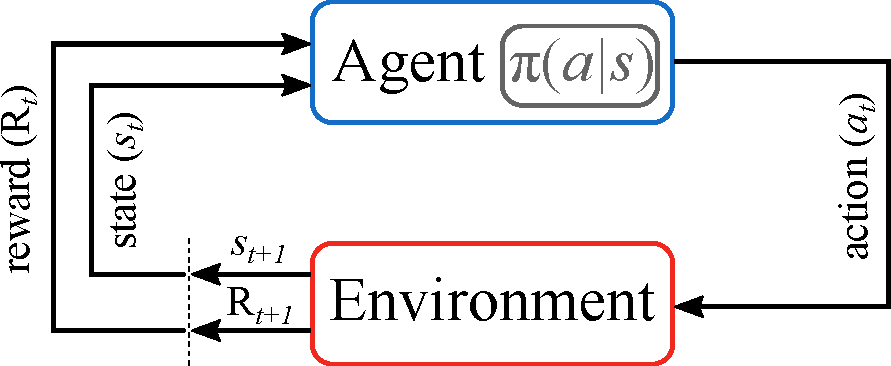
\includegraphics[width = 0.6\linewidth]{figures/RL_loop.pdf}
    \caption{Schematic of the typical learning loop for reinforcement learning agent. [Adapted from \citet{sutton2018reinforcement}]}
    \label{fig:RL_loop}
\end{figure}

In the previous description of the learning loop, $\mathcal{S}$, $\mathcal{A}$, and $\mathcal{R}$ correspond to the set of states, actions and rewards, respectively. These steps correspond to one cycle of the learning loop. The learning process extends for several cycles until a termination state is reached. The succession of cycles provides a repertory of actions and state observations ($s_t$ from now on for simplicity) that define a trajectory $\tau = (s_0,a_0,s_1,a_1,\dots)$. For each state, the agent looks for the optimal action to maximise its cumulative reward along the whole trajectory. In general, the targeted quantity is the discounted cumulative reward along a trajectory \citep{Viquerat2021RLrev}, defined as:
%
\begin{equation}
    R(\tau) = \sum_{t=0}^T \gamma^t r_t,
\end{equation}
%
where $T$ is the final time of the trajectory, and  $\gamma \in [0,1]$ is a discount factor to balance the relative importance of present and future rewards. The expected return is maximised through two possible approaches, namely value-based and policy-based methods. The former consist of determining the \textit{value function} \citep{sutton2018reinforcement} of a state-action pair, which is used to derive the following action to take at each state, while the latter directly aims at optimising a parameterised policy, which drives the agent performance.

A particularly successful application of RL is the resolution of games. The pioneering effort by \citet{Tesauro1992difflearn} describes a backgammon learner, in which the program started from no knowledge and trained by playing. After a million iterations, the program reached a performance similar to the best three human players in the world and won the computer backgammon olympiad \citep{BruntonNoackKoumoutsakos2020}. Recently, the development of neural networks allowed the application of RL to more complex games, such as Go \citep{mnih2015DRL} and the AI gym \citep{mnih2015DRL,Silver2016go}. RL is, however, a costly method due to the long learning process required to reach good performance. The acceleration of the learning process is a must for the application of RL to demanding scenarios, such as experiments and simulations of fluid flows \citep{Verma2018swimDRL}.

The agent does not only focus on revealing patterns in the environment dynamics or its actions but also aims at maximising the long-term rewards, which is the ultimate objective of RL methods. The long-term credit assignment (LTCA) implies assuming a certain relation between agent actions and environment rewards, which is derived from the trajectory of states and actions $\tau$. LTCA is still a major concern in RL. A common solution consists in modifying the original sparsely rewarded objective by adding highly rewarded sub-objectives \citep{schaul2015app}. Another challenge of RL is the correct use of information from experience by the agent when updated during the learning process \citep{Novati2019gliding}. In this regard, a proper tuning between \textit{exploration} and \textit{exploitation} is recommended. The agent must be able to find the optimal action by exploiting past experience while exploring alternative actions within the available solution space. Nonetheless, this is a common problem of several model-free algorithms.\\

Deep reinforcement learning (DRL) emerges from applying deep neural networks to model the agent. An artificial neural network (ANN), or simply neural network (NN), is a network of connected computational units, known as neurons, distributed in different layers that provides universal approximation capabilities \citep{Hornik1989MLP,Siegelmann1995NN}. For a fully connected network, each neuron receives input from all the neurons in the previous layer and feeds to all the neurons in the following layer. The neurons first compute the weighted sum of their inputs and, then, add a bias, which accounts for the output features that are independent of the input data. Eventually, the result from each neuron passes through a non-linear activation function that determines whether and to what extent the calculated value influences the final output. In DRL, NNs are trained to effectively map the relation between observations and actions \citep{rabault2019DRL}. This training process consists of the progressive adjustment of the biases and weights of the neural network towards the minimisation of a well-posed loss function that quantifies the network performance. The interested reader is referred to \citet{Goodfellow2016book} throughout the description of DRL.

In fluid mechanics, DRL has been recently applied to several problems to determine the parameters of control laws, such as swimming of fish schoolings \citep{gazzola2014RL}, control of unmanned aerial vehicles \citep{bohn2019DRL}, and optimization of glider trajectory taking ascendance \citep{reddy_learning_2016}. Most recently, DRL has been also applied to feedback-loop flow control like the wake control of a cylinder in simulations \citep{rabault2019DRL,rabault2019JFM} and in experiments \citep{Fan2020}, the tuning of the heat transport in a two-dimensional Rayleigh–Benard convection \citep{Beintema2020controlRBC}, and the wake stabilization past a cylinder by imposing a rotation on two control cylinders located at both sides \citep{Xu2020joh}.

\subsection{Policy-based methods} \label{ss:policymethods}
%
Policy methods rely on a \textit{policy} to drive the decision-making process of the agent. The final goal is to optimise the policy to maximise the expected discounted cumulative reward. The policy $\pi(a|s)$ is a mapping function based on a probability distribution over actions given a state rather than on a value function. Compared to value-based methods, policy-based methods ensure a better convergence, deal with high-dimensional action spaces, and exhibit great capabilities for learning stochastic policies \citep{Viquerat2021RLrev}. 

In fluid mechanics, most of the up-to-date applications of reinforcement learning prefer policy gradient methods, in which the parameterised policy $\pi_\theta(a|s)$ is optimised through a gradient ascent algorithm. The optimisation problem builds around the objective function, which is generally based on the expected discounted cumulative reward,
%
\begin{equation}
    J(\theta) = {\underset{\tau \sim \pi_\theta}{\mathbb{E}}}\left[ R(\tau) \right]
\end{equation}
%
to find the optimal set of parameters $\theta^*$ that maximises $J(\theta)$, namely
%
\begin{equation}
    \theta^* = {\underset{\theta}{\arg\max}}~{\underset{\tau \sim \pi_\theta}{\mathbb{E}}}\left[ R(\tau) \right]
\end{equation}

The optimisation problem could be directly solved by gradient ascent algorithm, considering an estimation of the policy gradient $\nabla_\theta J(\theta)$. The gradient with respect to the policy parameters $\theta$ is, however, a complex quantity to be determined. The common approach follows the log-probability trick \citep{Williams1992ML}, which derived $\nabla_\theta J(\theta)$ as an expected value that can be evaluated:
%
\begin{equation}
    \nabla_\theta J(\theta) = {\underset{\tau \sim \pi_\theta}{\mathbb{E}}}\left[ \sum_{t=0}^T \nabla_\theta \log(\pi_\theta(a_t|s_t)) R(\tau) \right],
\end{equation}

The evaluated gradient updates the policy parameters ($\theta \leftarrow \theta + \lambda  \nabla_\theta J(\theta)$, being $\lambda$ the learning rate) and the process repeats until convergence. The performance of policy gradient methods is jeopardised by the learning rate, which determines the step size in the gradient direction \citep{Viquerat2021RLrev}. Low learning rates translate into a long training process with no practical convergence whereas an excessive value of the learning rate could pass without heeding through the global optima, collapsing in a sub-optimal policy with poor performance. Proximal policy optimization \citep[PPO,][]{schulman_proximal_2017} relies on an effective heuristic to avoid destructive updates of the policy, i.e. it ensures restrained updates of the policy $\pi_\theta$, with respect to the previous $\pi_{\theta_{\text{old}}}$. The PPO method has drawn a lot of interest in the DRL community because of its increased learning stability and generally stable behaviour concerning hyperparameters. In fluid mechanics, early attempts to apply DRL for flow control focused on the simple problem of a shedding wake of a cylinder in simulations \citep{rabault2019JFM} and in experiments \citep{Fan2020}.

%------------------------------------------------------------------------------------------------
\section{Evolutionary Algorithms}

Optimization (and search) algorithms could be defined as learning algorithms featured by the determination of a probability distribution containing the relevant design aspects to optimise a given environment phenomenon \citep{BruntonNoackKoumoutsakos2020}. This conception was first envisioned by \citet{Schwefel1977}, introducing the concept of evolution strategies (ES) that later expanded to genetic algorithms \citep[GAs,][]{holland1992adaptation} and genetic programming \citep[GP,][]{Koza1994gp}, giving rise to the category of Evolutionary Algorithms (EA) in computational intelligence. Evolutionary algorithms or strategies build on the adaptation and progressive improvement of a set of candidate solutions inspired by biological evolution. Each potential solution is defined as an \textit{individual}, composing the \textit{population} that progressively evolves from one generation to the next. Darwin's ``evolution of species'' theory and its most recent updates and corrections describe the natural mechanisms governing the adaptation capability of individuals. The three main working principles of evolutionary algorithms derive from this knowledge \citep{duriez2017book,cornejomacedaPhD}, namely 
%
\begin{itemize}
    \item \textbf{survival of the best}: the most fitting or most performing individual, based on the environment requirements, prevails in the following generation. This mechanism guarantees the quality of incoming populations;
    \item \textbf{crossover}: mechanism to diversify the population by recombining individuals, which exploits the most performing features of the individuals;
    \item \textbf{mutation}: purely exploitative mechanism in which new individuals or features come up, ensuring uniqueness and freshness in following generations.
\end{itemize}
%
The recombination and mutation of individuals is a stochastic mechanism that guarantees the continuous exploitation and exploration of the most performing individuals within the solution space. Therefore, evolutionary algorithms may be thought of as crossbreeds between Monte Carlo sampling techniques, which explore the search space, and gradient search strategies, which exploit the best features toward a minimum.

Evolutionary algorithms can be used for flow control applications solving the optimisation problem in section~\ref{ss:optproblem}. The performance of each control law described by each individual is modelled by the cost function $J$ and the generation of individuals depends on the input data and the kind of algorithm. Under the umbrella of evolutionary algorithms, there is a wide variety of techniques to solve different types of problems. Some well-established examples are the genetic algorithms (GA) \citep{holland1992adaptation}, covariance matrix adaptation evolution strategy \citep{Hansen1996cmaes} or genetic programming (GP) \citep{Koza1994gp}. In this thesis, both GP and GA are considered in Papers 4 and 5, respectively. Both techniques stand on the same principle, mimicking natural processes; however, the definition of the individuals is different. GA identify the optimal individual as the best set of control parameters within the solution space, whereas GP derives a control law as a function of the input data, namely the sensor information. The control law provided by GP is commonly more complex and variable in time since it adjusts based on the state of the plant. GP represents a potent regression approach capable of re-discovering and combining flow control techniques without the need for physics knowledge in the circumstances of multi-frequency forcing and direct feedback control \citep{cornejomaceda2019pamm}.

GAs have been recently used to reduce the skin-friction drag in a TBL by optimising the phase delay among six streamwise-aligned slot jets \citep{Yu2021GA_drag_slot_jets},  to control the wake of a bluff body based on multi-frequency forcing \citep{minelli2020lgac}, and to optimise the performance of a spiral double-pipe heat exchanger \citep{Tian2020GAheatexchanger}, to name a few. In the field of heat transfer, the extensive review by \citet{Gosselin2009GareviewHT} describes many other successful applications of GA control. On the other hand, GP derives laws of low to medium complexity, such as the phasor control, threshold-level based control, periodic or multi-frequency forcing, including jet mixing optimization with pulsed jets at the nozzle exit \citep{zhou2020artificial}, drag reduction past bluff bodies \citep{li2019prf}, shear flow separation control \citep{gautier2015MLC}, reduction of vortex-induced vibrations of a cylinder \citep{Ren2019pof}, mixing layer control \citep{Parezanovic2016jfm}, and wake stabilization of complex shedding flows \citep{raibaudo2019pof}, among others.\\

The following section focuses on genetic programming, in particular in the Linear-based Genetic Programming (LGP) algorithm proposed by \citet{li2017GP} due to its greater degree of complexity compared to a classic GA. A brief description of the method and the learning process is provided. The interested reader on GAs is referred to \citet{holland1992adaptation} and \citet{Wahde2008book}.

\subsection{Genetic Programming}\label{ss:GP}
%
Genetic programming is an optimisation algorithm that proposes solution candidates as a computer program \citep{Koza1994gp}. These programs define the solutions in the form of a mathematical function of the input data, which could be used for several purposes such as fitting a surface, control laws or conditional decision making. In this section, this method is briefly introduced based on \citet{Wahde2008book}, \citet{duriez2017book} and \citet{cornejomacedaPhD}.

The internal representation of the mathematical function describing the control law is crucial to correctly applying the genetic operators. The classic classification distinguishes
%
\begin{itemize}
    \item \textbf{tree-based genetic programming}: the control law builds on a tree in which the nodes are the operators and the leaves are the operands \citep{duriez2017book}.
    \item \textbf{linear genetic programming (LGP)}: the control law is defined as a sequence of unitary or binary mathematical operations encoded in a matrix \citep{brameier2007linear}.
\end{itemize}
%
Despite sharing the same fundamental principle of operation, LGP is preferred in this thesis for its simplicity regarding multiple-input-multi-output (MIMO) control, since LGP deals with different input data and defines several control laws with only one matrix, and genetic operators, because mutation and crossover operations apply on the same matrix with simple combination or modification of individuals.

Linear genetic programming control (LGPC) is the application of LGP to solve control problems, deriving control laws as mathematical functions of the input data. The individuals, namely the control laws, are defined based on instructions, a register of variables and a set of constants \citep{duriez2014MLC}. The instructions combine input data through basic operations $(+,-,\times,\div,\sin,\text{exp},\text{\etc})$ to produce the control commands as outputs. Each individual, and its instructions, are represented by a 4-column matrix in which every row corresponds to an instruction. Columns 1 and 2 contain the register indices of the arguments, column 3 is the operator index, and column 4 is the output register. The registers are crucial in terms of memory management, distinguishing two types: \textit{variable registers} that can be overwritten during the execution of an instruction, commonly employed for intermediate calculations; and \textit{constant registers} that are preserved while the algorithms access the matrix data, which contain data of the problem or random constants. A potential problem of the matrix representation of the individual is the repetition of the same mathematical function after applying all the instructions, i.e. there is no unique matrix representation for a certain control law. A numerical test is performed before the evaluation of individuals in which repeated instances are discarded and replaced by a new one.

The combination of arguments and operators may yield instructions without any impact on the resultant control command, which is named \textit{introns}. These introns become crucial in the process of building relevant structures \citep{cornejomacedaPhD}. Nonetheless, the crossover and mutation operators may `activate' these instructions leading to an alteration of the resultant control law \citep{duriez2017book}. In principle, any mathematical function could be represented in matrix form if a sufficient number of instructions is considered together with a proper diversity in the operators' library. Not only that, but the library of input data plays a key role when building the proper control law. Eventually, the diversity of both libraries determines the complexity of the feasible solution space in the optimisation problem. \\

The LGPC process is described in the following as illustrated in figure~\ref{fig:GPC_algorithm}. The first step consists of a Monte Carlo optimisation through which a random sampling of individuals is used to generate the first population. Then, a tournament selection is carried out on the most performing individuals on which the genetic operations are performed to build the new generations. This process is repeated till convergence or when the stropping criterion is reached. Replication and elitism ensures the memory of the learning process while crossover and mutation exploit and explore over the solution space. The operator is chosen based on their respective probabilities ($P_c,P_m,P_r$), which are user-defined parameters that can be tuned to strengthen either the exploration or exploitation nature of the algorithm.

\begin{figure}
    \centering
    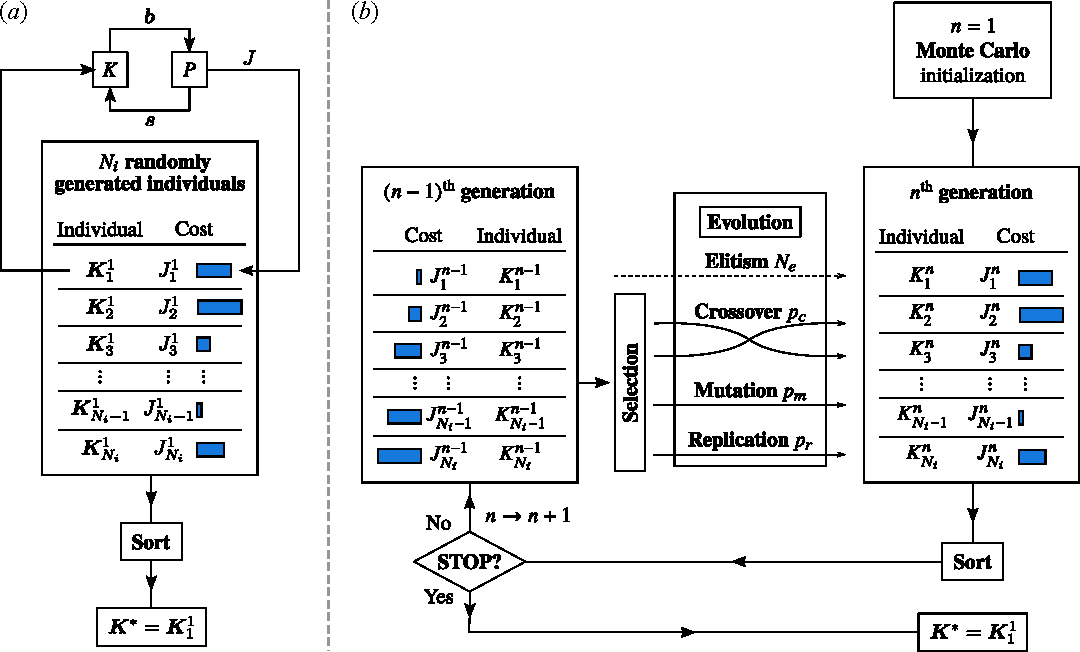
\includegraphics[width=0.99\linewidth]{figures/GPC_algorithm.pdf}
    \caption{(a) Monte Carlo sampling of the first generation. (b) Linear evolutionary algorithm. Each generation is built from the previous based on the genetic operators. \textit{Figures reproduced from \citet{cornejomacedaPhD} with permission of the author.}}
    \label{fig:GPC_algorithm}
\end{figure}

\subsubsection*{Monte Carlo optimisation}
Monte Carlo optimisation could, in principle, solve the flow control without the need for the evolutionary part; however, for a solution space with infinite dimensions, a multitude of individuals is required to ensure convergence toward the global optimum of the problem. LGPC considerably reduces the number of evaluations required for convergence, which becomes a limiting factor in real-life applications. The Monte Carlo optimization process provides the $N_i$ individuals of the first generation in the LGPC process by a random selection of operators and input data from the available libraries. Figure~\ref{fig:GPC_algorithm}(a) illustrate the Monte Carlo process for controlling a plant $P$ with the control law $K$ and control command $b$ (the reader is referred to section~\ref{ss:optproblem} for the definition of symbols). The maximum number of instructions and the number of variable and constant registers are user-defined parameters that the Monte Carlo sampling needs to comply with. The individuals are then evaluated and sorted based on their cost $J$. Eventually, the outcome of the algorithm is the most performing individual, i.e. the individual with the lowest cost.

\subsubsection*{Selection}
The genetic operations to build the incoming generations are performed on a certain set of individuals selected in a tournament selection process. The best $N_t$ individuals in the population are selected. The one that performs the best among them is picked with a probability of $P_t$. If not chosen, the same probability $P_t$ is used to select the second best and the process is repeated if needed for all the tournament individuals until the selection of the least performing. The user-defined parameters $N_t$ and $P_t$ influence the so-called \textit{selection pressure}, which is the degree to which high performers are chosen over low performers \citep{Wahde2008book}. Papers 4 and 5 in this thesis, for GP and GA respectively, follow the recommendations from \citet{duriez2017book}, setting $N_t = 7$ for a population of $N_i = 100$ individuals and $P_t = 1$.

\subsubsection*{Crossover for exploitation}
Crossover recombines individuals to extract the relevant features in the population. Thus, this is an exploitation operator through which two matrices split in two and swap, yielding two new individuals, namely the \textit{offsprings}.

\subsubsection*{Mutation for exploration}
The mutation is an exploitative operator to explore other features for a better control law. Each instruction has a certain probability to be randomly modified, which changes the matrix and, hence, leads to a new individual.

\subsubsection*{Replication and elitism for memory}
The most relevant features within a population are to be maintained for the incoming generation. Replication is the operator that copies individuals, ensuring the reminiscence of good individuals while enabling their future recombination. Similarly, the most performing individual during the process is always present in the latest generation due to elitism operator, preventing the loss of talent throughout the generations.

%
%===============================================================================
% Main contributions and Conclusions
%===============================================================================
%
%===============================================================================
\chapter{Main contributions and conclusions}\label{ch04}
%===============================================================================
%
The control of turbulence is a trendy research field with a potential expansion during the last decade thanks to the technological development hand in hand with novel algorithms based on artificial intelligence. This thesis aims at answering some of the numerous research questions within this exciting research area. This chapter gathers the main contributions and conclusions of the scientific publications performed in fulfilment of the objectives of this dissertation. For a more profound understanding and a detailed discussion of the results, the reader is referred to the appended papers in Part II of the present document.

The research work under the scope of this thesis deals with the control of turbulent boundary layers to manage the convective heat transfer at the wall. Starting from the exploration of well-known actuation mechanisms in other applications, such as skin-friction reduction or mixing enhancement, two parametric studies were performed to shed light on the flow mechanisms behind wall heat fluxes. As described in Chapter~\ref{ch02}, among the variety of available actuation systems, both plasma actuators and jets in crossflow were considered. In paper 2, a spanwise array of streamwise DBD-plasma vortex generators is used to reduce heat transfer. The experimental results confirm a considerable alteration of the flow topology due to the formation of pairs of counter-rotating streamwise vortices embedded in the boundary layer. An effective 10\% reduction in convective heat transfer is achieved. On the other hand, the spanwise slot jet in Paper 3 is used to enhance heat transfer. After the parametric study on the pulsation parameters, a simplified model is proposed decoupling the effect of the carrier frequency and duty cycle. A characteristic frequency of the system is found at which heat transfer enhancement is magnified. Although the justification of the optimality remains an open research question, flow field measurements revealed the development of large-scale turbulent structures in the near-wall region, which promote entrainment and mixing, hence enhancing heat transfer.

Seeking a more sophisticated control logic, the performance of machine-learning-based algorithms is evaluated in Paper 4. This article compares deep reinforcement learning and linear genetic programming control on a benchmark problem to assess their performance when varying the initial condition provided to the controller and in the presence of noise. In general, DRL outperforms LGPC; however, LGPC achieves significantly more compact and interpretable control laws, identifying subsets of the probes as being relevant to defining control actions. The numerical investigation concludes that RL and LGPC are up-and-coming flow control techniques, although LGPC seems more robust and implementable for practical applications. Based on this gained experience, Paper 5 deals with an experimental TBL control for heat transfer enhancement in which the control logic is given by linear genetic algorithms. The open-loop control problem can find the same characteristic frequency as in Paper 3, which corroborates its importance to maximize heat transfer.

%===============================================================================
%- Paper Highlights
%===============================================================================
\section{Paper highlights}
%-------------------------------------------------------------------------------
This section highlights the contributions of each of the papers included in the present thesis.\\

\noindent {\bf  Paper~1. Methodological.} \\
\noindent {\sc  Castellanos, R., Sanmiguel Vila, C., G\"uemes, A. \& Discetti, S.}{, 2021. }{\it  \let \\=~On the uncertainty of boundary-layer parameters from Ensemble PTV data . }{{Meas. Sci. Technol.}}{ {\bf  32}}{ (8)}{, 084006}.

\begin{itemize}
 \item An uncertainty quantification framework for turbulent boundary layer characterisation based on ensemble particle tracking velocimetry (EPTV) measurements is developed for the first time.
  \item The effect of systematic errors due to finite spatial resolution and of random error due to convergence are investigated under different window sizes.
  \item The uncertainty on the TBL parameters depends on the bin size used in the EPTV process expressed in wall units.
\end{itemize}
\vspace{.5cm}

%-------------------------------------------------------------------------------
\noindent {\bf  Paper~2.} \\
\noindent {\sc  Castellanos, R., Michelis, T., Discetti, S., Ianiro, A. \& Kotsonis, M.}{, 2022. }{\it  \let \\=~Reducing turbulent convective heat transfer with streamwise plasma vortex generators. }{{Exp. Therm. Fluid Sci.}}{ {\bf  134}}{, 110596}.

\begin{itemize}
  \item A turbulence control experimental investigation is presented based on a spanwise array of streamwise DBD-plasma actuators vortex generators. The plasma actuators induce the formation of pairs of streamwise counter-rotating vortices embedded in the turbulent boundary layer. 
  \item The plasma-induced vortices considerably alter the topology of the incoming flow. The geometry of the plasma actuator, together with its suction-injection mechanism, encloses the vortices in the spanwise direction, making them stationary and persistent far downstream.
  \item Heat transfer is effectively reduced downstream of the actuation with a maximum average reduction of 9\% in the Stanton number. The Stanton number scales with the 2/7 power of the momentum coefficient.
\end{itemize}
\vspace{.5cm}

%-------------------------------------------------------------------------------
\noindent {\bf  Paper~3.}\\
\noindent {\sc  Castellanos, R., Salih, G., Raiola, M., Ianiro, I. \& Discetti, S.}{, 2022. }{\it  \let \\=~Heat transfer enhancement in turbulent boundary layers with a pulsed slot jet in crossflow. }{{Appl. Therm. Eng.}}{ {\bf  Under review}}.

\begin{itemize}
    \item A spanwise jet in crossflow is used to enhance convective heat transfer at the wall within a turbulent boundary layer. A parametric study on the pulsation frequency and the duty cycle is performed.
    \item The duty cycle is the parameter driving the injection of air and hence scales the overall heat transfer enhancement. Lower duty cycles lead to more cost-effective actuations for the maximization of convective heat transfer.
    \item The convective heat transfer enhancement can be decoupled into two independent functions of the pulsation parameters.
    \item A characteristic frequency of the dynamic system that maximizes the heat transfer is found.
    \item The jet in crossflow induces a wall-tangent jet and a pair of counter-rotating vortices that increase momentum fluxes in the lower region of the boundary layer.
\end{itemize}
\vspace{.5cm}

%-------------------------------------------------------------------------------
\noindent {\bf  Paper~4.} \\
{\sc  Castellanos, R., Cornejo-Maceda, G. Y., de la Fuente, I., Noack, B. R., Ianiro, I. \& Discetti, S.}{, 2022. }{\it  \let \\=~Machine learning flow control with few sensor feedback and measurement noise. }{{Phys. Fluids}}{ {\bf  34}}{ (4)}{, 047118}.

\begin{itemize}
  \item Wake control based on Deep Reinforcement Learning (DRL) and Linear Genetic Programming Control (LGPC) is assessed for a two-dimensional K\'{a}rm\'{a}n vortex street past a cylinder. Similar performance is observed in the absence of noise and for the fixed initial condition.
  \item DRL shows higher robustness to variable initial conditions and noise contamination of the sensor data.
  \item  LGPC identifies compact and interpretable control laws, which only use a subset of sensors, thus allowing reducing the system complexity with reasonably good results.
\end{itemize}
\vspace{.5cm}

%-------------------------------------------------------------------------------%
\noindent {\bf  Paper~5.} \\
{\sc  Castellanos, R., Ianiro, I. \& Discetti, S.}{, 2022. }{\it  \let \\=~Genetically-inspired convective heat transfer enhancement. }{{Exp. Therm. Fluid Sci.}}{ {\bf  Submitted}}.

\begin{itemize}
    \item Machine learning control is used to optimise the convective heat transfer enhancement in a turbulent boundary layer on a flat plate.
    \item The optimised control outperforms the steady-jet actuation with less power requirement.
    \item The best control law induces an asymmetry in the flow field caused by the phase between actuators.
    \item A characteristic pulsation frequency of the dynamic system that maximizes the heat transfer is found. Such frequency is approximately the inverse of the characteristic travel time of large-scale turbulent structures convected within the buffer layer.
\end{itemize}
%-------------------------------------------------------------------------------

%===============================================================================
%- Future work
%===============================================================================-
\section{Future work}
%-------------------------------------------------------------------------------
Despite the insightful discussion and explanation of the physical phenomena behind heat transfer processes in the aforementioned investigations, the ultimate contribution of this thesis is proof of the feasible implementation of sophisticated machine-learning algorithms in an experimental environment together with complex measurement techniques for turbulence. Although DRL, LGPC and LGAC have been previously tested in experimental investigations, Paper 5 is the first study in which IR thermography is used to update the controller. The sophistication of the experimental apparatus and the software orchestrating the learning loop foreshadows the unavoidable implementation of a feedback signal for real-time closed-loop control.

Several interesting research lines may arise from the conclusions drawn in this thesis. Some of the possible future investigations are listed below:

\begin{itemize}
    \item The implementation of closed-loop control in which the actuation is driven by the feedback signal provided by sensors. For this purpose, it is already planned to use microphones embedded in the wall and placed upstream of the slot jets. The training process is divided into two loops: the learning loop, in which the controller is updated based on the cost function, and the control loop, in which the instantaneous actuation is adjusted based on the sensor signal. In the latter, the agent or control law is unaltered and runs in real-time, while the former is the actual learning cycle of the algorithm, which is not required to be real-time for certain applications as shown in Paper 5.
    \item Although this thesis is mainly experimental, it is interesting to test other control algorithms in a numerical environment. The numerical simulations are a perfect test bench for sophisticated algorithms. In particular, two possible control logics are proposed: (1) the use of three-dimensional convolutional neural networks to envision more complex control laws; and (2) the implementation of a reduced-order modelling together with a machine learning control algorithm, pursuing the best control law in the low-dimensional subspace.
    \item Application of the gained experience and knowledge to other flow configurations. In particular, it is already planned to implement the control on two base flows: a turbulent jet, targeting noise reduction, and a bluff body for wake suppression and drag reduction. 
\end{itemize}
%
%===============================================================================
% References
%===============================================================================
%
\bibliographystyle{jfm}
\bibliography{overview/overview}
%
\IfFileExists{overview/overview.bbl}{\graphicspath{{imgs/}}

%===============================================================================
% Introduction
%===============================================================================
%
\input{overview/ch01-introduction}
%
%===============================================================================
% Methodology
%===============================================================================
%
\input{overview/ch02-HTcontrol}
\input{overview/ch03-MLC}
%
%===============================================================================
% Main contributions and Conclusions
%===============================================================================
%
\input{overview/ch04-contributions}
%
%===============================================================================
% References
%===============================================================================
%
\bibliographystyle{jfm}
\bibliography{overview/overview}
%
\IfFileExists{overview/overview.bbl}{\input{overview/overview.bbl}}{}
}{}
}{}



%-------------------------------------------------------------------------------
% Comment the following command if you do not want a separate page for Part II
% in the table of contents
%
\tocpagebreak


%===============================================================================
% Part II: Papers
%===============================================================================
%
\part{Scientific Journal Publications}
%-------------------------------------------------------------------------------
% Summary of the papers
%
\makepapersummary
\cleardoublepage

%-------------------------------------------------------------------------------
% Paper 1: Uncertainty EPTV
%------------------------------------------------------------------------------
% Define title, author(s), affiliation and publishing status
%
\papertitle[On the uncertainty of BL parameters from EPTV data] % Short title used in headlines (optional)
{%
  On the uncertainty of boundary-layer parameters from Ensemble PTV data % THE COMMENT SYMBOL AT THE END OF THIS LINE IS NEEDED
}%
%
\papertoctitle{On the uncertainty of boundary-layer parameters from Ensemble PTV data} % Title for toc
%
\paperauthor[R. Castellanos \etal] % Short authors used in headlines and List Of Papers
{%
  R. Castellanos$^1$, C. Sanmiguel Vila$^1$, A. G\"uemes$^1$ \& S. Discetti$^1$%
}%
%
\listpaperauthor{Castellanos, R., Sanmiguel Vila, C., G\"uemes, A. \& Discetti, S.}% (optional) Short authors used in List Of Papers
%
\paperaffiliation
{%
  $^1$ Aerospace Engineering Research Group, Universidad Carlos III de Madrid (UC3M), Avda. Universidad, 30, 28911 Leganes, Madrid, Spain\\
}%
%
\paperjournal[Meas. Sci. Technol.] % Short publish info used in List Of Papers
{%
	Measurements Science and Technology%
}%
%
\papervolume{32}%
%
\papernumber{8}%
%
\paperpages{084006}%
%
\paperyear{2021}%
%
% \paperdoi{10.1088/1361-6501/abfad0}
%
\papersummary%
{% Insert summary of the paper here (used in introduction)
    The recent advancements in high-resolution turbulent-statistics computation from ensemble particle tracking velocimetry (EPTV) data are now opening new possibilities in turbulent-flow characterisation. Measurements of full-field boundary layer profiles with a fine resolution close to the wall and up to the freestream with one single imaging setup are now feasible, thus paving {the way} to direct characterisation of turbulent-boundary-layer (TBL) parameters with composite-profile formulations. In this work, we build a framework for the estimation of the uncertainty of EPTV in performing this task. The effect of systematic errors due to finite spatial resolution and of random error due to convergence are investigated under different window size. {Then we introduce random errors to simulate the effects on convergence issues on the velocity profile and, consequently, on the estimation of turbulent-boundary-layer parameters. The statistical dispersion of the estimated parameters provides an estimation of the uncertainty range.} We validate with experimental data {this} flexible tool to estimate \textit{a priori} the expected uncertainty level of the most relevant {turbulent-boundary-layer} parameters in zero-pressure-gradient TBL, being the method based on existing profiles from high-fidelity simulation or from analytical {composite-profile} formulations when such data are not available.
}%
%
\graphicspath{{paper1/}}%
%
%
%===============================================================================
%                            BEGIN PAPER
%===============================================================================
%
\begin{paper}

\makepapertitle

%------------------------------------------------------------------------------
% Abstract
%------------------------------------------------------------------------------
%
\begin{paperabstract}
    The recent advancements in high-resolution turbulent-statistics computation from ensemble particle tracking velocimetry (EPTV) data are now opening new possibilities in turbulent-flow characterisation. Measurements of full-field boundary layer profiles with a fine resolution close to the wall and up to the freestream with one single imaging setup are now feasible, thus paving {the way} to direct characterisation of turbulent-boundary-layer (TBL) parameters with composite-profile formulations. In this work, we build a framework for the estimation of the uncertainty of EPTV in performing this task. The effect of systematic errors due to finite spatial resolution and of random error due to convergence are investigated under different window size. {Then we introduce random errors to simulate the effects on convergence issues on the velocity profile and, consequently, on the estimation of turbulent-boundary-layer parameters. The statistical dispersion of the estimated parameters provides an estimation of the uncertainty range.} We validate with experimental data {this} flexible tool to estimate \textit{a priori} the expected uncertainty level of the most relevant {turbulent-boundary-layer} parameters in zero-pressure-gradient TBL, being the method based on existing profiles from high-fidelity simulation or from analytical {composite-profile} formulations when such data are not available.
    \keywords{ensemble particle tracking velocimetry, PIV, turbulent boundary layer, wall-bounded flows}
\end{paperabstract}


%------------------------------------------------------------------------------
% Article
%------------------------------------------------------------------------------
%
\definecolor{blue}{rgb}{0,0,1}
\definecolor{red}{rgb}{1,0,0}
\definecolor{black}{rgb}{0,0,0}
\definecolor{grey}{rgb}{0.5,0.5,0.5}
\definecolor{dark}{rgb}{0.25,0,0.37}
\definecolor{orange}{rgb}{0.58,0.08,0.3}
\definecolor{yellow}{rgb}{1,0.59,0}
\definecolor{purple}{rgb}{0.92,.24,0.18}
\definecolor{blue1}{rgb}{0.81,0.9,0.95}
\definecolor{blue2}{rgb}{0.65,0.81,0.91}
\definecolor{blue3}{rgb}{0.38,0.69,0.83}
\definecolor{blue4}{rgb}{0.13,0.56,0.76}
\definecolor{blue5}{rgb}{0,.39,0.67}
\definecolor{blue6}{rgb}{0,.25,0.5}
\section{Introduction}
Accurately determining the parameters that describe an experimental turbulent boundary layer (TBL) is crucial to modelling and understanding these flows \citep{titchener2015calculation,pan2020unscented}. In particular, the parameters that can be employed to characterise the mean velocity profile of a TBL can be used, among other purposes, to determine whether a TBL can be considered as well-behaved, (i.e. not in a post-transitional state or affected by non-equilibrium effects) \citep{Chauhan:2009p10824,Sanmiguel:2017JFM}, to compare the results between different experimental or numerical datasets \citep{Schlatter:2009p13969} or to calculate dimensionless numbers that are used to analyse the effect of disturbances such as the inclusion of obstacles or pressure gradients \citep{Clauser:1954p10911,guemes2019flow}. These parameters include quantities such as: the friction velocity $u_\tau$, defined as $u_\tau = \sqrt{\tau_w/\rho}$ (being $\tau_w$ the mean wall-shear stress and $\rho$ the fluid density); the boundary layer thickness $\delta$, which is the wall-normal distance beyond which viscous effects can be considered as negligible; and the freestream velocity $U_\infty$. Among the classical TBL parameters it is also common to define the so-called integral lengths, such as the displacement thickness $\delta^*$ and the momentum thickness $\theta$, providing information regarding the mass and momentum transfer within the boundary layer. The integral lengths are defined for an incompressible flow as,
\begin{equation}
    \delta^* = \int_{0}^{\infty} \left(1-\frac{U}{U_\infty}\right) \,dy;
\end{equation}
\begin{equation}
 \theta = \int_{0}^{\infty} \frac{U}{U_\infty}\left(1-\frac{U}{U_\infty}\right) \,dy.
\end{equation}

being $U = U(y)$ the velocity distribution as a function of the wall-normal coordinate $y$. Since in turbulent boundary layers, $U$ does not {necessarily reach an asymptotic value} at the boundary-layer edge, the previous formulation can be truncated at the boundary layer thickness $\delta$ for its upper integration limit such that,
\begin{equation}
\label{integral}
    \delta^* = \int_{0}^{\delta} \left(1-\frac{U}{U_e}\right) \,dy;~~ \theta = \int_{0}^{\delta} \frac{U}{U_e}\left(1-\frac{U}{U_e}\right) \,dy
\end{equation}
and in consequence the boundary-layer edge velocity is defined as $U_e = U(y=\delta)$.

Using the previously defined TBL parameters, it is possible to generate new figures of merit, such as the shape factor defined as $H_{12}=\delta^*/\theta$ or the skin-friction coefficient $C_f = \tau_w/(\frac{1}{2} \rho U_\infty^2)$, that allow the assessment of the flow regime or discern whether a particular TBL can be considered to be canonical \citep{Chauhan:2009p10824}. Such quantities are used due to their high sensitivity to different boundary and inflow conditions \citep{Chauhan:2009p10824}.

Regardless of the measurement technique, these boundary-layer parameters are  strongly affected by errors due to discretization of the velocity profile, the spacing between the points, the distance of the first point from the wall, and uncertainty in the wall location \citep{titchener2015calculation,Orlu:2010p36071}. In addition to these sources of error, there is no consensus when it comes to the methodology for calculating $\delta$. Several of the proposed methods rely on the use of additional quantities besides the mean velocity profile, such as the mean vorticity \citep{spalart1993experimental}, the mean streamwise variance \citep{Vinuesa:2016is} or a reference pressure \citep{griffin2020general}. On the other hand, accurate determination of friction-related quantities (such as $u_\tau$ and $\tau_w$) is also particularly challenging \citep{orlu2020instantaneous}. Different experimental approaches that can be employed to measure these quantities, such as oil-film interferometry \citep{Vinuesa:2016tn}, Preston tube \citep{head1962preston},  MEMS shear-stress sensor \citep{sheplak2004mems}.

For {the particular case of zero-pressure gradient (ZPG) TBLs and in} those situations where only mean streamwise velocity measurements are available, an alternative to calculate all the boundary-layer parameters is to resort to composite velocity profiles based on analytical expressions \citep{Chauhan:2009p10824,Coles:2006p898,Nickels:2004p15662,Rodriguez-Lopez2015}. This methodology is based on assuming that the mean streamwise velocity profile can be described using a function that takes the form of $U^+(y^+)= U^+_{inner}+U^+_{outer}$, which is used to fit the data of the aforementioned profile. In the present study the superscript $+$ denotes inner scaling, which is defined as $U^+=U/u_\tau$ and $y/\ell^*$, being $\ell^*$ the viscous length $\ell^* = \nu/u_\tau$ and $\nu$ the kinematic viscosity. The term $U^+_{inner}$ is the part of the function that provides a description of the velocity profile from the viscous sublayer up to the overlap region, while the term $U^+_{outer}$ is used to define the outer region of the TBL profile. The $U^+_{inner}$ function is typically based on $U^+=y^+$ for the inner region and on the logarithmic law $U^+=\frac{1}{\kappa}y^+ +B$ for the overlap region, where $\kappa$ is the von Kármán constant and $B$ is an integration constant. The $U^+_{outer}$ function was introduced by \citet{Coles:2006p898} with the inclusion of the wake function $\mathcal{W}$, defining the wake component of the velocity profile. There are different formulations of the wake function since the wake component is greatly affected by boundary or initial conditions. Depending on the study, the complexity of the $U^+$ formulation can be varied and even some of the parameters can be previously defined from established correlations to reduce the dimensionality of the fitting process. The major advantage of this methodology is that, by using just a full-resolution mean velocity profile, it is possible to estimate the {boundary-layer} parameters and to correct the wall location. 

Hardware and software advances have recently opened the path to full-resolution {TBL velocity-profile} measurements at sufficiently large friction Reynolds number using Particle Image Velocimetry (PIV). In particular, techniques based on ensemble averaging (e.g. single-pixel correlation \citep{westerweel2004single}, or ensemble particle tracking velocimetry, EPTV \citep{cowen1997hybrid,kahler2012uncertainty}) are able to achieve a sufficiently large dynamic range to resolve the entire velocity profile, from the viscous sublayer up to the freestream, thus enabling {composite-profile} application. Single-pixel correlation is based on ensemble averaging of cross-correlation maps. EPTV is based on identifying vectors from instantaneous realisation and superposing them to build a dense cloud of vectors. Statistical information is then inferred from the pdf of the velocity vectors in averaging windows, referred as \textit{bins} (either isotropic, anisotropic or with shape adapted locally \citep{raiola2020adaptive}). 
Reynolds stresses can also be measured accurately if velocity gradient effects within the averaging bin are taken into account. In single-pixel correlation, this can be achieved by proper modelling of the shape of the cross-correlation peak \citep{scharnowski2012reynolds}, while in EPTV the velocity-gradient effect can be reduced by local polynomial fitting of the vectors to be averaged \citep{aguera2016ensemble}. It was recently shown in mild {adverse-pressure-gradient TBLs} \citep{SanmiguelVila2017} that this second approach is generally more robust; furthermore, the recent advances in volumetric velocimetry \citep{discetti2018volumetric} are now pushing towards a widespread use of Lagrangian Particle Tracking (LPT), thus motivating an increased interest in understanding the capabilities of EPTV approaches in measuring velocity profiles. PIV/PTV offer the indisputable advantage of providing also information on the instantaneous flow field organisation; this renders worth exploring the uncertainty of PIV/PTV/LPT in determining parameters which are normally measured using the portfolio of techniques mentioned above.

In this work, the uncertainty in extracting boundary-layer parameters from ``full-field'' EPTV data is explored, i.e. assuming that the field of view covers the entire {boundary-layer} thickness plus a robust freestream measurement. {For the sake of simplicity, the present study is focused on well-behaved ZPG TBLs in which a composite-profile approach can be applied, as in hot-wire measurements.} While it is common to use separate experiments for high-resolution near-wall measurements (see for instance the work by \citet{kahler2006wall}) and for the {full-field} organisation, the approach we present here has the advantage of requiring the same image dataset for statistics extraction and flow field characterisation.
We will first simulate in virtual experiments the effect of finite spatial resolution on data generated from Direct Numerical Simulations (DNS) of a {ZPG TBL} and using a composite profile {formulation of a ZPG TBL}. Systematic errors due to the bin-averaging effect and the position of the first measurement point with respect to the wall are addressed in \S \ref{s:SyntheticValidation} as a function of the bin size. {In this section random errors due to finite convergence or wall-positioning uncertainty are not introduced, as the focus is simply on systematic error.}

Then {in \S \ref{s:validation}} a {Monte Carlo} study is conducted to estimate the uncertainty of the composite profile fitting due to finite number of samples. This is particularly relevant in EPTV, since the bin size depends on the number of snapshots and the number of vectors within the bin, considered sufficient for a satisfactory accuracy. {The method will thus deliver an uncertainty range for each turbulent-boundary-layer parameter. An experimental validation is carried out to verify that the error on the ZPG TBL parameters are predicted within an uncertainty range for a wide range of bin sizes.} 

%--------------------------------------------------------------------------------
%------------------------------- METHODOLOGY ------------------------------------
%--------------------------------------------------------------------------------
\section{Methodology}
The methodology to estimate the uncertainty of EPTV measurements for TBL characterisation is illustrated in this section. The method is based on simulating the errors due to finite resolution and convergence on existing TBL profiles, either based on DNS {ZPG} data or on analytical formulation of {ZPG TBL} composite profiles. Different levels of camera resolutions and bin sizes are explored in order to investigate systematic errors in the fitting procedure and the random uncertainty due to convergence issues. {In the proposed method no particle images are generated; the effects of the error sources are directly simulated by averaging existing velocity profiles (or generated ad hoc with composite profile formulations). This renders the method of simple and general application, avoiding the need of generating virtual images for the specific case.}

\subsection{Synthetic profile generation} \label{ss:synthetic_method}

The synthetic TBL profile is generated from existing datasets to replicate the incurred errors from experiments using EPTV. The synthetic profile is generated using as a reference:

\begin{itemize}
    \item Dataset of {ZPG TBL} DNS simulations, available in the turbulent database of the Fluid Dynamics Group from Universidad Politécnica de Madrid\footnote{\url{https://torroja.dmt.upm.es/turbdata/blayers/}}. In particular, for the analysis conducted in the following, the data corresponding to $Re_{\vartheta}=4500$ have been used \citep{sillero2013one}.
    \item Composite-profile generated data based on the ZPG TBL formulation by \citet{Chauhan:2009p10824} which will be briefly outlined in \S \ref{s:composite_profile}.
\end{itemize}

{The velocity vectors are directly generated from the interpolation of the DNS data in the first case, and from the analytical formulation of the composite profile in the second case.} In all cases, the simulated field of view spans from the wall to $1.3\delta$. This upper bound is set in order to guarantee a sufficiently robust measurement of the freestream. The resolution is here defined in wall units as {$Res = \frac{S}{1.3 Re_\tau}$}, being $S$ the available pixels in the camera sensor in the wall-normal direction. 

The systematic error due to bin averaging in the binning process of the EPTV is simulated by top-hat averaging of the velocity profiles within bins of different size. We tested bin sizes ranging between {$1\ell^*$ to $200\ell^*$}. The bin size distribution in wall units is reported in Figure \ref{fig:window} as a function of the size in pixels and of the spatial resolution expressed in pixels per wall unit.

The profiles are truncated removing from the near-wall region bins which were not completely included in the domain. While this would imply removing vectors with distance from the wall smaller than one half of the window size, after the analysis of the experimental results, we decided to introduce a more restrictive criterion and cut the profiles to a distance of 3/4 of the window size. This criterion excludes from the analysis pixels in close proximity from the wall, which are very likely to be affected by spurious reflection effects in PIV measurements. Due to the sensitivity of the composite-profile formulation to the quality of the near-wall data, this criterion was found to be more robust. 

The effect on the streamwise mean velocity profile of the bin averaging is shown in Figure~\ref{fig:F1_DNSprofiles} for DNS data. The effect of increasing the bin size is clear in the near-wall region, where the measured profile departs from the baseline due to averaging effects. It is expected that this systematic error, combined with the lack of points in the near-wall region for relatively large bin size, will yield more significant errors in determining the friction velocity and the wall position. Also, the computation of integral quantities is sensitive to the position of the nearest point to the wall \citep{titchener2015calculation,Rodriguez-Lopez2015}. 

\begin{figure}
    \centering
    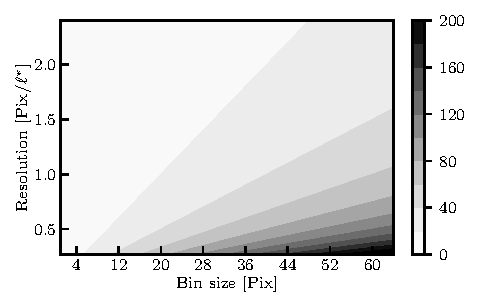
\includegraphics[width=0.75\columnwidth]{Figures/figure08.pdf}
    \caption{Bin size distribution {expressed in wall units $l^*$} with respect to bin size in pixels and resolution.}
    \label{fig:window}
\end{figure}


\begin{figure}
    \centering
    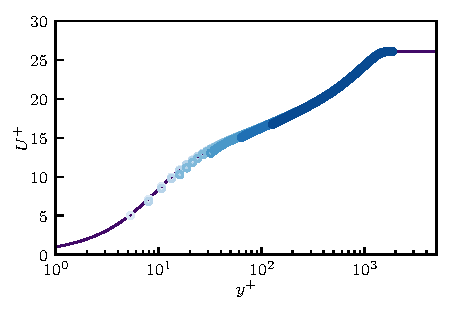
\includegraphics[width=0.75\columnwidth]{Figures/figure05.pdf}
    \caption{Effect on the streamwise mean velocity profile of the bin averaging in EPTV with 2 \sy{blue1}{o}, 4 \sy{blue2}{o}, 8 \sy{blue3}{o}, 16 \sy{blue4}{o}, {32} \sy{blue5}{o}, and 64 \sy{blue6}{o} pixels bin size for a fixed value of $S=700$. Ground truth DNS data is referred as \lcap{-}{dark}.}
    \label{fig:F1_DNSprofiles}
\end{figure}

Two contributions of random error have been included. The first error is a perturbation of the initial guess of the wall position, which is most often inferred from visual inspection of the images. This process might be severely affected by the image quality near the wall; furthermore, depending on the surface material and quality, the wall position might not be completely clear. {Throughout this work} we introduced a uniformly distributed random error with bounds $\pm0.5$ pixels, even though the presented uncertainty estimation method can be tuned to model more optimistic/pessimistic scenarios. The second contribution of random error is due to convergence, which depends on the random error on the velocity vectors (assumed here having Gaussian distribution with standard deviation $\sigma_v$) and on the turbulent fluctuation levels. If we indicated with $u'$ the standard deviation of the streamwise turbulent fluctuations, the expected standard deviation of the error of the mean is:
\begin{equation}
\label{ruido}
    \sigma_{U}=\frac{\sqrt{u'^2+\sigma_v^2}}{\sqrt{N_v}}    
\end{equation}
with $N_v$ being the number of vectors in each bin (supposing for simplicity it is sufficiently small to ensure that on average it contains less than 1 vector per snapshot). 
For the DNS data, the profile of $u'$ is available and can be directly plugged in Eq.~\ref{ruido}; however, for the case simulated with the composite profile proposed by \citet{Chauhan:2009p10824}, since an analytical formulation for second-order statistics is not readily available, the standard deviation of the error of the mean is modelled assuming a two-level distribution with piecewise constant $u'$. A level of $u'^+=2$ for $y<0.9 \delta$ is chosen as an average value of the streamwise turbulent fluctuations for the $Re_\tau$ under study and a value of $u'^+=0.5$ as a representative value of the freestream velocity is used for the locations $y\geq 0.9 \delta$.

A {Monte Carlo} approach is followed to characterise the uncertainty on the estimation of the {ZPG }TBL parameters. The systematic and random uncertainty are defined respectively using the median and the standard deviation of the results of the simulated experiments. {The systematic errors are addressed in \S \ref{s:SyntheticValidation}, while the effect on random uncertainty is introduced in \S \ref{s:validation}.}

\subsection{Calculation of the boundary-layer parameters}
\label{s:composite_profile}

In order to calculate the different boundary-layer parameters and to correct the wall location using only the mean streamwise velocity profile, a two-step strategy based on the use of two different composite profiles is followed. In a first step, the mean velocity data after the EPTV process is fitted to the composite profile proposed by \citet{Chauhan:2009p10824} {for ZPG TBLs }and defined as follows,

\begin{equation} \label{eq:chauhan}
U^+=U^+_{inner}+\frac{2\Pi}{\kappa} \mathcal{W} \left( \eta \right), 
\end{equation}
being $\Pi$ the wake parameter and $\eta=y^+/\delta^+$. Using this formulations the $U^+_{inner}$ and $\mathcal{W}\left(\eta \right)$ read as follows,

\begin{equation}
\label{innerchuahan}
\begin{array}{ll}
U^+_{inner}=& \frac{1}{\kappa} \ln\left(\frac{y^+-a}{-a}\right)  + \frac{R^2}{a(4\alpha+a)} 
 (4\alpha+a)  \\
& \left[ \ln \left(-\frac{a}{R}\frac{\sqrt{(y^+ -\alpha)^2+\beta^2}}{y^+-a}\right) +\frac{\alpha}{\beta}(4\alpha+5a) \right. \\
& \left. \left(\arctan\left(\frac{y^+-\alpha}{\beta}\right)+\arctan\left(\frac{\alpha}{\beta}\right)\right) \right]+ \\ &\frac{\exp[-\ln^2(y^+/30)]}{2.85},
\end{array}
\end{equation} 
where $\alpha=(-1/\kappa-a)/2$, $\beta=\sqrt{-2a\alpha-\alpha^2}$, $R=\sqrt{\alpha^2+\beta^2}$, $\kappa=0.384$ and $a=-10.3061$. The wake function $\mathcal{W}$ is defined as,

\begin{equation}
\label{outerchauhan}
\begin{array}{ll}
\mathcal{W}(\eta)= & \frac{1-\exp\left[-(1/4)(5a_2+6a_3+7a_4)\eta^4+a_2\eta^5 +a_3\eta^6+a_4\eta^7
	\right]}{1-\exp[-(a_2+2a_3+3a_4)/4]}  \\
& \times \left(1-\frac{1}{2\Pi}\ln(\eta)\right) 
\end{array}
\end{equation} 
where $a_2=132.8410$, $a_3=-166.2041$ and $a_4=71.9114$. The values of the constants have been derived by \citet{Chauhan:2009p10824} from several experiments over a large Reynolds number range and their formulation has been tested and proved to be robust when it comes to identify well-behaved profiles  \citep{Chauhan:2009p10824}. This composite-profile formulation is used to determine the values of $u_\tau$ and to correct the absolute wall position correction $\Delta y $ by means of a least-square procedure \citep{Chauhan:2009p10824,Orlu:2010p36071,Rodriguez-Lopez2015}. Since the values of the constants are fixed, this formulation allows to calculate $u_\tau$ without relying on locating the overlap region.

In the second step, the extracted values of $u_\tau$ and $\Delta y$ are used to calculate the corresponding $U^+$ and $y^+$ and then fit them to the composite profile proposed by \citet{Nickels:2004p15662}, which has the following formulation for the particular case of a {ZPG TBL}, 

\begin{equation}
\label{Nickels}
\begin{array}{lll}
U^+ = & y^+_c \left[1- (1+2(y^+/y_c^+)+\frac{3}{2}(y^+/y^+_c)^2)e^{-3y^+/y_c^+}  \right] \\
& \times \frac{1}{6\kappa
_0} \left(\ln(\frac{1+(0.6(y^+/y_c^+))^6}{1+\eta^6})+b(1-e^{-\frac{5(\eta^4+\eta^8)}{1+5\eta^3}})\right) 
\end{array}
\end{equation} 
in which $b$ is a measure of the wake strength and is equivalent to wake parameter, $\kappa_0=0.39$ and $y_c^+=12$. 
This composite profile is used for the calculation of the edge velocity $U_e$ and the boundary-layer thickness $\delta$ because of its description of the wake region. The wake function proposed by \citet{Nickels:2004p15662} has been proved to be robust at low Reynolds numbers for both experimental and numerical profiles \citep{Schlatter:2010p35519}. Eventually, the resulting fitted velocity profile is integrated according to Eq.~\ref{integral} and using the $\delta$ and $U_e$ for the integration limits to extract $\delta^*$ and $\theta$. 

\section{Systematic error estimation for synthetic data}
\label{s:SyntheticValidation}

\begin{figure}
    \centering
    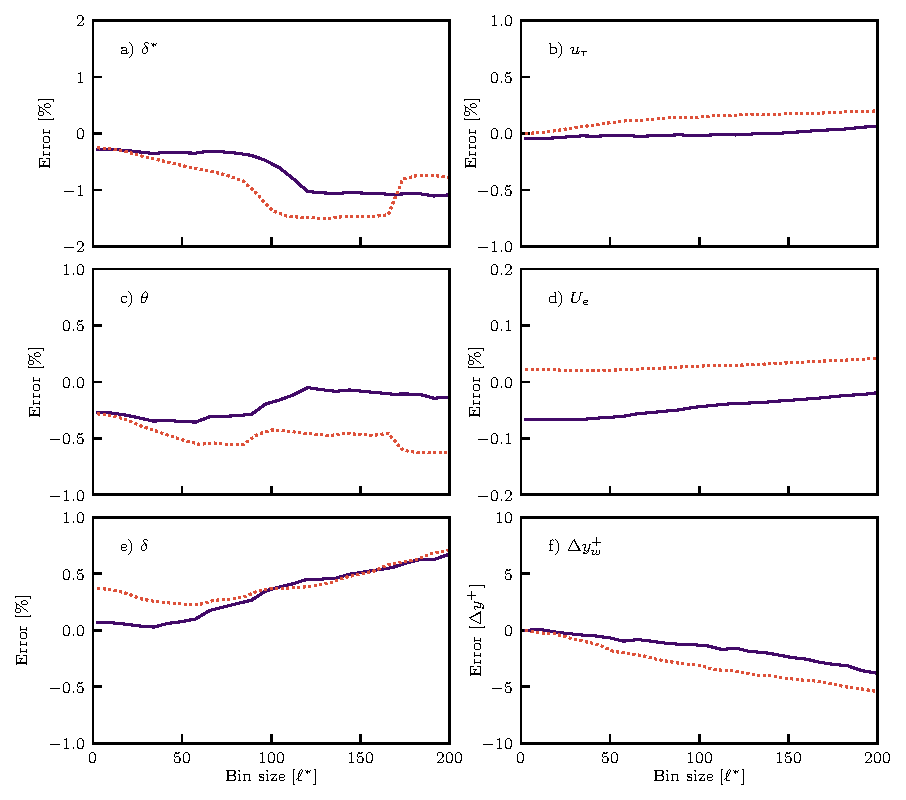
\includegraphics[width=\textwidth]{Figures/figure09.pdf}
    \caption{Systematic error as a function of the bin size for a) displacement thickness, b) friction velocity, c) momentum thickness, d) freestream velocity, e) boundary layer thickness, and f) y origin. Symbols refer to DNS \lcap{-}{dark}, Composite-profile \lcap{:}{purple}.}
    \label{fig:systematic_error}
\end{figure}

The procedure described in \S\ref{ss:synthetic_method} is explored {for different bin size in wall units}. {The objective of this section is to explore the systematic error due to the filtering effect on the profile due to finite bin size.} For this reason, the error sources due to convergence and to the wall-normal coordinate are not considered. Therefore, {the computation of TBL parameters} is performed {averaging on} a reduced set of {50} cases with a small random perturbation on the velocity profile ($N_v \sim O(10^6)$) to avoid bias errors due to locking in local minima in the fitting optimization procedure described in \S\ref{s:composite_profile}.

As reported in Figure~\ref{fig:F1_DNSprofiles}, the size increase of the averaging bin promotes two main effects on the velocity profile: the suppression of valid points in the near-wall region based on the criterion describes in \S\ref{ss:synthetic_method}; and the diversion of the near-wall points of the profile. 
As the {bin} size increases, at certain point, the averaging process in the logarithmic region will be affected by points within the buffer region, which eventually tend to curve the profile. As a consequence, the slope of the velocity profile in the logarithmic region will not follow the logarithmic law. This strongly affects the fitting procedure proposed by \citet{Chauhan:2009p10824}, especially for a proper estimation of the wall location and the friction velocity, since it assumes a velocity profile which fulfils the logarithmic law of the wall.

An overview of the performed parametric study is reported in Figure~\ref{fig:systematic_error}, based on data generated according to DNS of a TBL and the composite profile described in \S\ref{s:composite_profile}, respectively. The relative error is computed with respect to the reference parameters reported in Table~\ref{tab:1}.

The systematic error {profiles as a function of the bin size in wall units} are overall consistent between DNS and composite-profile data. This is particularly interesting since the composite profile can be easily generated for conditions matching the experiments, while high-fidelity simulations data might not be available, especially at high Reynolds numbers.

For the parameters computed from the first fit based on \citet{Chauhan:2009p10824}, i.e. $u_\tau$ and $\Delta y^+$, we observe a clear tendency of increasing magnitude of the error as the averaging bin increases in size. Nonetheless, the systematic error in $u_\tau$ estimation does not exceed 1\% and the correction of wall-normal coordinate is below $5^+$ for bin size smaller than {100}$\ell^*$. This result {suggests} that, although the bin size will affect the performance in the estimation of the parameters, the composite profile proposed by \citet{Chauhan:2009p10824} is robust in the inner region of the velocity profile. Only when the bin size affects the logarithmic layer, the fit is not capable of correcting for the wall position with an acceptable level of accuracy. {It is important to remark here that the estimation of $u_\tau$ with the composite profile is robust since the data correspond to ZPG conditions. In presence of pressure-gradient, curvature, roughness or other effects it is well known that the composite profile is less robust and the availability of points in the near-wall region becomes of paramount importance.} 

For the TBL parameters estimated in the second step by using the fit proposed by \citet{Nickels:2004p15662}, we find $\delta^*$ and $\theta$, with a relatively low error for {bin} sizes that lie below the logarithmic region; however, as the bin size exceeds 50$\ell^*$, the error becomes more significant. This is a direct consequence of the curvature smoothing effect promoted by the top-hat averaging as shown in Figure~\ref{fig:F1_DNSprofiles}, which is reducing the effectiveness of the second {inner} fit. Additionally, we find a systematic overestimation of both $\delta$ and $U_e$ {for the composite-profile case (although for the case based on the DNS profile $U_e$ appears to be slightly underestimated)}. This might be surprising at a first glance, since averaging effects are much less relevant at the edge of the boundary layer. This suggests that the truncation and bias errors in the near-wall region of the TBL are also affecting the results of the composite-profile fitting in the outer region. 

\begin{table}
\centering
% table caption is above the table
\caption{\centering Reference TBL parameters for DNS, composite profile and experiments.}
\label{tab:1}       % Give a unique label
% For LaTeX tables use
\resizebox{\textwidth}{!}{%
\begin{tabular}{lcccccccccc}
\hline\noalign{\smallskip}
 Case & $Re_{\tau}$ & $Re_{\theta}$ & $H_{12}$ & $\delta^*/\delta$ & $\theta/\delta$ & $u_{\tau}$[m/s] & $U_{e}$ [m/s] & $\delta$ [mm]  & $\ell^*$ [$\mu$m] & $C_f \cdot 10^3$\\
\noalign{\smallskip}\hline\noalign{\smallskip}
DNS          & 1437 & 4500 & 1.381 & 0.169 & 0.122 & - & -& - & - & 2.98 \\
{Composite-profile}        & 1445 & 4503 & 1.375 & 0.165 & 0.120 & 0.70  & 18.14 & 32 & 22 & 2.98\\ 
Experiments          & 1379 & 4432 & 1.390 & 0.170 & 0.123 & 0.042 & 1.11 & 29 & 21 & 2.91\\
\noalign{\smallskip}\hline
\end{tabular}}
\end{table}

\section{{Random uncertainty measurements - }experimental Validation} \label{s:validation}

{In this section the capabilities of the proposed methods to estimate the uncertainty range of each TBL parameter are tested. For this purpose, differently to the previous section, random errors on the velocity profiles due to finite convergence and wall-positioning are included, with a number of vectors per bin matching experimental conditions. A large number of tests is carried out to obtain statistics of the errors on the TBL parameters, thus delivering uncertainty ranges for each of them. An experimental validation is carried out using a high-resolution ZPG-TBL measurement as ground truth, and investigating the error introduced when increasing the bin size.}

\subsection{Experimental setup}

\begin{figure}
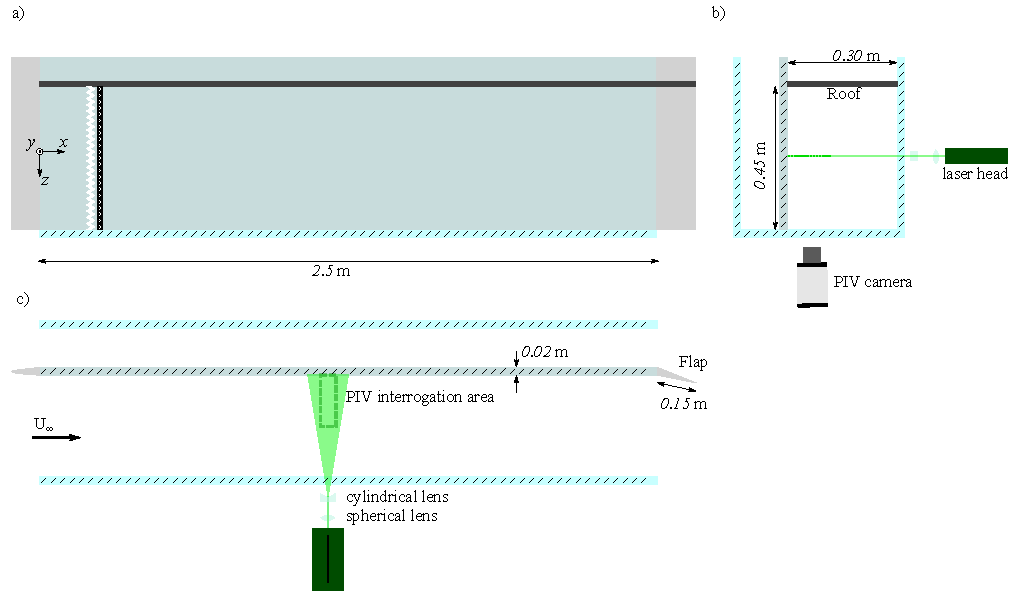
\includegraphics[width = 0.99\linewidth]{Figures/setup.pdf}
\caption{Sketch of the experimental setup. The flat plate is indicated in cyan, the walls of the water tunnel in light blue, and the 3D printed leading edge and flap in grey. a) Frontal view with reference system. The zig-zag tripping and dymo strips are included for reference. b) Lateral view, with illumination and imaging system. c) Top view, with optical arrangement and PIV measurement area.
}\label{fig:expsetup}
\end{figure}



An experimental campaign is held in the water tunnel at Universidad Carlos III de Madrid. The facility has a rectangular test section ($500 \times 550$~mm$^2$) with a length of $2.5$~m. A sketch of the experimental setup is reported in Figure~\ref{fig:expsetup}.  A flat plate is vertically mounted in the water tunnel, spanning the entire test section length. The flat plate is equipped with additively-manufactured leading edge of ratio 5:1 and trailing-edge flap of 150~mm chord to ensure the location of the stagnation point. The boundary layer is tripped 0.1~m downstream of the leading edge with a zig-zag turbulator of $1.5$~mm height, followed by a V-embossed tape which has a nominal height of 0.3 mm. The measurements are conducted at a single streamwise station located at approximately $x=1.1$~m from the leading edge. A characterisation of the turbulent-boundary-layer behaviour has been conducted to ensure that a nearly zero-pressure-gradient condition is achieved, and that the boundary layer is well-behaved in the location of the measurement \citep{Sanmiguel:2017JFM}. For such purpose, the working-fluid viscosity is characterised with an Ostwald viscosimeter calibrated with distilled water. Viscosity is measured several times in order to reduce as much as possible the random uncertainty, with a standard deviation below 0.5\%.

The setup for PIV measurements is sketched in Figure~\ref{fig:expsetup}b-c. The flow is seeded with neutrally-buoyant polyamide particles ($10$~$\mu m$ diameter). Illumination is provided by a dual cavity Nd:Yag Quantel Evergreen laser ($200$~mJ/pulse at $15$~Hz), shaped into a laser sheet with thickness of $1$~mm. A 5.5 MPixels Andor sCMOS camera is equipped with a $50$~mm and a $100$~mm lenses to capture two datasets with different resolution (respectively about 25~pix/mm and 65~pix/mm, corresponding to a magnification of 0.16 and 0.42 and an inner-scaled resolution of 0.52~pix/$\ell^*$ and  1.34~pix/$\ell^*$). The two datasets will be referred in the following as low-resolution (LR) and high-resolution (HR) dataset. In the LR dataset a region of $300 \times 1650$ pixels is imaged, corresponding to $ 12 \times 66$~mm$^2$. For the HR dataset the image format was $300 \times 2450$ pixels, corresponding to about $ 4.6 \times 38$~$mm^2$. For both datasets the streamwise extension of the imaged domain is sufficiently small (less than $\delta/2$) to ensure statistical homogeneity (thus allowing averaging in the streamwise direction), while the wall-normal size of the field of view is larger than $\delta$, thus ensuring a robust measurement of the freestream and a full-view of the velocity profile. 

In both cases 28.000 images are captured, with a particle image density of approximately $1.6\cdot10^{-3}$ and $0.5\cdot10^{-3}$ particles per pixel for the LR and HR dataset, respectively. The relatively low seeding density ensures that the probability of spurious particle pairing and the errors due to particles overlap are minimised. Nonetheless, the strong velocity gradients in the near-wall region combined with the limited image density reduce the robustness of the predictor in the near-wall region, thus reducing the number of paired particles.  

\begin{figure}
    \centering
    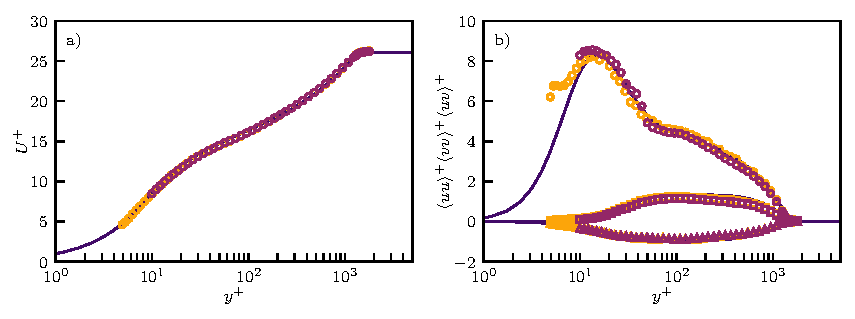
\includegraphics[width=\textwidth]{Figures/figure04.pdf}
    \caption{Profiles of the inner-scaled (a) mean velocity, and (b) Reynolds stresses of the velocity fluctuations. Colours refer to DNS \lcap{-}{dark}, EPTV - LR \lcap{-}{orange}, and EPTV - HR \lcap{-}{yellow}. In (b), symbols refer to streamwise \sy{black}{o}, wall-normal \sy{black}{s}, and shear \sy{black}{t} stresses.}
    \label{fig:F2_EPTVvsDNS}
\end{figure}


\subsection{Data processing}
A preprocessing is performed to remove the background and the laser reflection; the procedure is based on the eigenbackground subtraction described by \citet{Mendez2017181}. A super-resolution approach \citep{keane1995super} is followed to pair particle images in the captured dual-frames. The predictor velocity fields are obtained through image digital correlation \citep{willert1991digital}, based on a multi-pass \citep{soria1996investigation} image deformation algorithm \citep{scarano2001iterative} with a B-spline interpolation \citep{Astarita2005}. The final interrogation window is equal to 32 pixels with 75\% overlap region. Particle locations are identified with local maxima identification and Gaussian interpolation of the peak to achieve sub-pixel accuracy. The thresholding to identify whether a local maximum is a genuine peak is based on image statistics - only peaks above the local mean intensity plus one standard deviation are retained in the process. Particle images are then paired using a Kd-tree algorithm \citep{Tagliasacchi2021} for efficient pairing, with search biased by the PIV predictor. 

\subsection{EPTV and data post-processing} \label{ss:EPTV}
The ensemble averaging of the EPTV process is carried out on rectangular windows, with width of $200$ pixels and height variable between $3$ and $32$ pixels. A preliminary inspection of the wall reflection on the image allows to identify any misalignment between the camera reference system and the wall, and rotate the velocity vectors and averaging bins accordingly. Since the typical error in identifying manually the wall-position is of the order of the pixel size, the uncertainty of this procedure is below 0.5 degree.

On the streamwise direction an overlap of $80\%$ between the averaging windows is adopted. In the wall-normal direction initially a logarithmic grid has been adopted, with $50$ points from $1$ pixel above the wall up to $300$ pixels from the top of the image. In the last $300$ pixels a linear spacing has been adopted to obtain a robust estimate of the freestream. The profiles to be fitted with the composite profile are computed by averaging in the streamwise direction. A preliminary computation of the statistics has been carried out with the composite profile on the cases with window of $200\times3$ pixels (from now on named the reference cases for the LR and HR datasets using the full set of 28000 images). The results for the reference TBL are reported in Table~\ref{tab:1}. Additionally, the experimental reference cases are depicted in Figure~\ref{fig:fig01} against DNS data. 

The data are interpolated on a common grid based on the estimated $Re_\tau$ and wall position. The common grid is based on 70 logarithmically-spaced points from 0.1 wall units to {$0.9Re_\tau$},
and 20 linearly-spaced points from $0.93\delta$ to $1.3\delta$. This ensures that effects due to grid differences between the two datasets are removed.

The statistics computation is carried out by straightforward extraction of the statistical moments with equal weights on all vectors within the bin. While the polynomial approach by \citet{aguera2016ensemble} will improve the results close to the wall, it would not be comparable with the uncertainty estimation method presented in the previous section. Since the object of this work is to demonstrate the capability of our method to predict the uncertainty of the turbulent boundary layer parameters, we leave this aspect for future investigation.


\begin{figure}
    \centering
    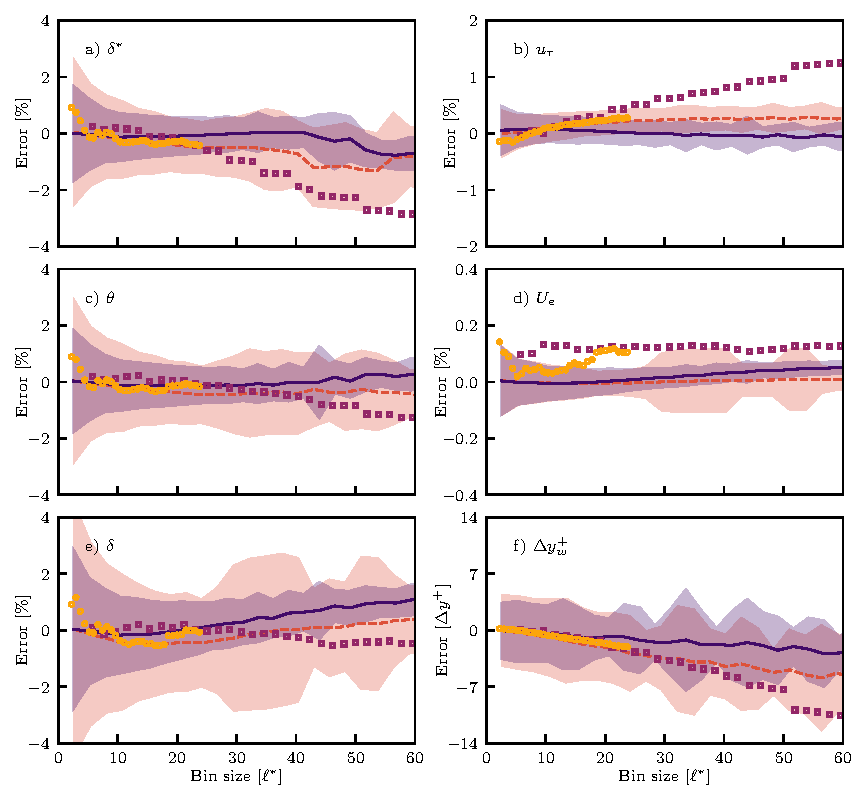
\includegraphics[width=\textwidth]{Figures/figure11.pdf}
    \caption{Comparison of error with respect to window size for a) displacement thickness, b) friction velocity, c) momentum thickness, d) freestream velocity, e) boundary layer thickness, and f) y origin. Symbols refer to DNS \lcap{-}{dark}, {Composite-profile} \lcap{--}{purple}, EPTV - LR \sy{orange}{s}, and EPTV - HR \sy{yellow}{o}. Error bars in DNS and {Composite-profile} refer to 3$\sigma$.}
    \label{fig:fig01}
\end{figure}


\subsection{Results}
\label{ss:expresults}

To compare the results among the experimental and the synthetic cases, the calculation of the profiles for the synthetic profiles has been carried out by setting the same resolution of the experiments. The averaged profiles are interpolated in the common grid described in \S\ref{ss:EPTV} to ensure the elimination of error sources due to grid differences between experimental and synthetic data.
Additionally, the estimation of TBL parameters is now performed by adding the random errors to the velocity profile and the {wall-normal} component. A total of 2000 runs are performed, and the standard deviation for each computed parameter is quantified to determine the corresponding uncertainty bars. 

The random error due to convergence is introduced as described in \S.\ref{ss:synthetic_method}, according to Eq.~\ref{ruido}. The TBL parameters are then computed using 2000 and 5000 images for the LR and HR dataset. The number of vectors $N_v$ is set equal to $350\cdot w$, with $w$ being the averaging bin size, to match the number of vectors observed in the dataset. The error of the experimental data is then estimated by using as a reference the velocity profile obtained using the full dataset of 28.000 images with window size of $200\times3$ pixels.

In Figure \ref{fig:F2_EPTVvsDNS} a comparison among the two experimental cases described in \S\ref{s:validation} and the DNS profile used as synthetic data is shown. Both experimental cases show an excellent agreement not only in the mean streamwise velocity profile (Figure \ref{fig:F2_EPTVvsDNS}a) but also in the different Reynolds stress components  (Figure \ref{fig:F2_EPTVvsDNS}b) up to the near-wall peak. For the high-resolution EPTV case, a deviation in the inner peak is appreciated which can be attributed to the residual reflections on the experimental images \citep{SanmiguelVila2017}. 

Figure \ref{fig:fig01} shows the relative error in the different boundary-layer parameters as a function of the bin size expressed in inner units. To normalise the error contribution, the resulting values of the {boundary-layer} quantities after fitting the original DNS profile, the Chauhan composite profile and the mean velocity profiles calculated using the full image data dataset (28.000 images) are employed. For the case of the quantities obtained by means of the composite profile proposed by \citet{Chauhan:2009p10824}, $u_\tau$ and $\Delta y^+$, it is observed for both quantities an error behaviour which, as expected, is equivalent to the error curves observed when analysing the effect of the first $y_0^+$ point available in hot-wire measurements \citep{Chauhan:2009p10824,Orlu:2010p36071,Rodriguez-Lopez2015}. For bin size values up to $\approx 12^+$, the error in both quantities is relatively small compared with the reference employed which is associated with profiles that have a $y_0^+<10$. When this bin size is exceeded, the error for both experimental cases shows much larger values. This effect is probably related to the higher levels of error in the logarithmic region for the experimental cases compared to the synthetic cases{, i.e. due to the strong local velocity profile curvature the PIV predictor for particles pairing is more prone to error}. For the quantities obtained by using the composite profile of \citet{Nickels:2004p15662} $\delta$, $U_e$, $\delta^*$ and $\theta$, the error curves are more robust and the agreement between the experimental data and the synthetic data is observed up to a bin size value of $\approx 25^+$. This corresponds to the location where there is no more inner points available and therefore all the estimation is performed based on the buffer and logarithmic region. It has to be noted that $U_e$ is slightly shifted in the error curves with respect to the reference. %As a consequence of the large number of images employed in the reference case (28.000), a more converged $U_e$ value is obtained compared to the error points which are calculated with only 2.000 images and therefore are more likely to be affected by the freestream disturbances.
This systematic error is quite small and might be to other minor issues, such as small drift of the flow conditions over the test time.

\section{Conclusions}

A method to estimate the uncertainty of {ZPG-}TBL parameters with the composite-profile based on data from full-field EPTV has been assessed. The proposed method is based on using data from simulations or composite profiles to reproduce the errors due to {wall-position} identification uncertainty, finite spatial resolution due to bin averaging and convergence due to finite number of samples. The synthetic and experimental validation demonstrate that the errors and uncertainty estimated using high-fidelity simulations and the composite-profile formulation are in good agreement, and predict accurately the range of error to be expected in the corresponding experiments. Simulation data can be more precise in determining the convergence limits since the streamwise velocity variance profile is well defined; on the other hand the approach based on the composite profile is more flexible, since it guarantees the possibility to closely match all the experimental conditions, including the Reynolds number.

The proposed approach can be used to:
\begin{enumerate}
    \item investigate systematic errors (as in \S\ref{s:SyntheticValidation}) by reproducing the same conditions to be expected in the experiments in terms of resolution and window size. It can be thus a useful tool to identify the requirements in terms of imaging before the experiments, and in principle it could also be used to reduce systematic errors.
    \item estimate the uncertainty range for the ZPG-TBL parameters. In this case, in addition to the spatial resolution and window size, the number of vectors per bin should also be included in the analysis to address errors due to convergence of the statistics. In this sense, this approach can be used also as an \textit{a priori} inference of the uncertainty, thus being useful to relate it quantitatively with the bin size and the number of vectors contained in it.
\end{enumerate}

\noindent{}It has to be remarked that this study is not including other sources of uncertainty which might be larger in an experiment than those quantified here, such as, for example, the uncertainty on the optical magnification. Furthermore, any departure from the condition of well-behaved ZPG TBL will determine additional uncertainty related to the suitability of the composite profile to fit the velocity profile. This is particularly delicate for quantities that are more sensitive to the quality of the near-wall region, such as $u_\tau$ or the wall position. 
Nonetheless, if any independent assessment of such additional uncertainty is available, the outcome of the uncertainty estimation approach proposed here can be used as input for the computation of combined uncertainties. \\

\section*{Code availability}
{The MATLAB\textregistered  codes for the calculation and plotting of the presented results are available from the repository \url{github.com/eaplab/EPTVuncertainty.git}. Camera-ready version of the figures have been generated with \url{github.com/guemesturb/TheArtist.git}.}

\section*{Acknowledgements}
RC, CSV and SD were partially supported by the Grant DPI2016-79401-R funded by the Spanish State Research Agency (SRA) and European Regional Development Fund (ERDF).


%------------------------------------------------------------------------------
% Bibliography
%------------------------------------------------------------------------------
%
%\clearpage
\bibliographystyle{jfm}
\bibliography{paper1/bib1}
%
\IfFileExists{paper1/bib1.bbl}{\input{paper1/bib1.bbl}}{}

%===============================================================================
%                            END PAPER
%===============================================================================
\end{paper}

%-------------------------------------------------------------------------------
% Paper 2: Plasmas
%------------------------------------------------------------------------------
% Define title, author(s), affiliation and publishing status
%
\papertitle[Reducing turbulent convective HT with streamwise plasma VG] % Short title used in healines (optional)
{%
Reducing turbulent convective heat transfer with streamwise plasma vortex generators% THE COMMENT SYMBOL AT THE END OF THIS LINE IS NEEDED
}%
%
\papertoctitle{Reducing turbulent convective heat transfer with streamwise plasma vortex generators} % Title for toc
%
\paperauthor[R. Castellanos \etal] % Short authors used in headlines and List Of Papers
{%
  Rodrigo Castellanos$^{1}$, Theodoros Michelis$^2$, Stefano Discetti$^1$, Andrea Ianiro$^1$ \& Marios Kotsonis$^2$%
}%
%
\listpaperauthor{Castellanos, R., Michelis, T., Discetti, S., Ianiro, A. \& Kotsonis, M.}% (optional) Short authors used in List Of Papers
%
\paperaffiliation
{%
  $^1$ Aerospace Engineering Research Group, Universidad Carlos III de Madrid, Legan\'{e}s 28911, Spain\\%
  $^2$ Department of Aerodynamics, Delft University of Technology, Delft 2629HS, The Netherlands. \\%
}%
%
\paperjournal[Exp. Therm. Fluid Sci.] % Short publish info used in List Of Papers
{%
	Experimental Thermal and Fluid Science%
}%
%
\papervolume{134}%
%
%\papernumber{1}
%
\paperpages{110596}%
%
\paperyear{2022}%
%
\papersummary%
{% Insert summary of the paper here (used in introduction)
The effect of streamwise plasma vortex generators on the convective heat transfer of a turbulent boundary layer is experimentally investigated. A Dielectric Barrier Discharge (DBD) plasma-actuator array is employed to promote pairs of counter-rotating, streamwise-aligned vortices embedded in a well-behaved turbulent boundary layer over a flat plate. The study aims at elucidating the mechanism of interaction between the plasma-induced vortical structures and the convective heat transfer process downstream of them. The full three-dimensional mean flow field is measured with planar and stereoscopic PIV. The convective heat transfer is assessed with infrared thermography over a heat-flux sensor located downstream of the actuators. The combination of the flow field and heat transfer measurements provides a complete picture of the fluid-dynamic interaction of plasma-induced flow with local turbulent transport effects. The results show that the streamwise vortices are stationary and confined across the spanwise direction due to the action of the plasma discharge. Flow-field measurements show that the opposing plasma discharge causes a mass- and momentum-flux deficit within the boundary layer, leading to a low-velocity region that grows in the streamwise direction and which is characterised by an increase in displacement and momentum thicknesses. This low-velocity ribbon travels downstream, promoting streak-alike patterns of reduction in the convective heat transfer distribution. Near the wall, the plasma-induced jets divert the main flow. This phenomenon is a consequence of the DBD-actuator momentum injection and, thus, the suction caused on the surrounding fluid by the emerging jets. The stationarity of the plasma-induced vortices makes them persistent far downstream, reducing the convective heat transfer.
}
%
\graphicspath{{paper2/}}%
%
%
%===============================================================================
%                            BEGIN PAPER
%===============================================================================
%
\begin{paper}

\makepapertitle

%------------------------------------------------------------------------------
% Abstract
%------------------------------------------------------------------------------
%
\begin{paperabstract}
	The effect of streamwise plasma vortex generators on the convective heat transfer of a turbulent boundary layer is experimentally investigated. A Dielectric Barrier Discharge (DBD) plasma-actuator array is employed to promote pairs of counter-rotating, streamwise-aligned vortices embedded in a well-behaved turbulent boundary layer over a flat plate. The study aims at elucidating the mechanism of interaction between the plasma-induced vortical structures and the convective heat transfer process downstream of them. The full three-dimensional mean flow field is measured with planar and stereoscopic PIV. The convective heat transfer is assessed with infrared thermography over a heat-flux sensor located downstream of the actuators. The combination of the flow field and heat transfer measurements provides a complete picture of the fluid-dynamic interaction of plasma-induced flow with local turbulent transport effects. The results show that the streamwise vortices are stationary and confined across the spanwise direction due to the action of the plasma discharge. Flow-field measurements show that the opposing plasma discharge causes a mass- and momentum-flux deficit within the boundary layer, leading to a low-velocity region that grows in the streamwise direction and which is characterised by an increase in displacement and momentum thicknesses. This low-velocity ribbon travels downstream, promoting streak-alike patterns of reduction in the convective heat transfer distribution. Near the wall, the plasma-induced jets divert the main flow. This phenomenon is a consequence of the DBD-actuator momentum injection and, thus, the suction caused on the surrounding fluid by the emerging jets. The stationarity of the plasma-induced vortices makes them persistent far downstream, reducing the convective heat transfer.

        \keywords{Heat transfer, DBD Plasma actuator, Turbulent Boundary Layer, Streamwise vortex}
\end{paperabstract}


%------------------------------------------------------------------------------
% Article
%------------------------------------------------------------------------------
%


%%%%%%%%%%%%%%%%%%%%%%%%%%%%%%%%%%%%%%%%%%%%%
%\usepackage{mylines}
%\usepackage{myplots}
%%% Plots style
%\newcommand{\sy}[2]{\mbox{(\kern-.25em\SymbolRGB[solid]{#1}{.8pt}{#2}{4pt}\kern-.25em)}}
%\newcommand{\linesy}[3]{\mbox{(\kern-.1em\lineSymbolRGB{#1}{#2}{1.5pt}{#3}{4.5pt}\kern-.45em)}}
%\newcommand{\lcap}[2]{~\,{\kern-1em\protect\mylcap{#1}{#2}}}
%\newcommand{\lincW}[1]{\textcolor{#1}{\rule[3pt]{.4cm}{2pt}}}
%\newcommand{\lsq}[1]{{\protect\lincW{#1}}}
%% Color definition
\definecolor{blue}{rgb}{0,0,1}
\definecolor{red}{rgb}{1,0,0}
\definecolor{black}{rgb}{0,0,0}
\definecolor{white}{rgb}{1,1,1}
\definecolor{grey}{rgb}{0.5,0.5,0.5}
\definecolor{dark}{rgb}{0.25,0,0.37}
\definecolor{yellow}{rgb}{1,0.59,0}
\definecolor{purple}{rgb}{0.92,.24,0.18}
\definecolor{sPIV}{rgb}{0,0.3059,0.7176}
\definecolor{pPIV}{rgb}{0.902,0.1569,0}
% Plasma actuator sketch
\definecolor{plasma}{rgb}{0.6196,0.2627,0.5176}
\definecolor{kapton}{rgb}{0.9961,0.5647,0.0}
\definecolor{electrode}{rgb}{0.302,0.302,0.302}
% Blues:
\definecolor{blue1}{rgb}{0.65,0.80,0.90}
\definecolor{blue2}{rgb}{0.50,0.69,0.86}
\definecolor{blue3}{rgb}{0.38,0.69,0.83}
\definecolor{blue4}{rgb}{0.13,0.56,0.76}
\definecolor{blue5}{rgb}{0,.39,0.67}
\definecolor{blue6}{rgb}{0,.25,0.5}
\definecolor{blue7}{rgb}{0,.15,0.3}
%%%%%%%%%%%%%%%%%%%%%%%%%%%%%%%%%%%%%%%%%%%%%%
% Commands for the table (green +) and (red -)
\definecolor{rr}{HTML}{FE0000}
\definecolor{gg}{HTML}{009901}
\newcommand{\red}[1]{\textcolor{rr}{#1}}
\newcommand{\green}[1]{\textcolor{gg}{#1}}

%%%%%%%%%%%%%%%%%%%%%%%%%%%%%%%%%%%%%%%%%%%%%%%%%%%%%%%%%%%%%%%%%%%%%%%%%%%%%%%
%%%%%%%%%%%%%%%%%%%%%%%%%%%%%%% INTRODUCTION %%%%%%%%%%%%%%%%%%%%%%%%%%%%%%%%%%
%%%%%%%%%%%%%%%%%%%%%%%%%%%%%%%%%%%%%%%%%%%%%%%%%%%%%%%%%%%%%%%%%%%%%%%%%%%%%%%
\section{Introduction}
A common solution for convective heat transfer enhancement in turbulent flows consists of producing embedded streamwise vortices in the boundary layer \citep{jacobi1995} by the use of passive elements such as vortex generators \citep{Zhaoqing2019VG} or wall-mounted obstacles \citep{nakamura2001cube,mallor2018cubes}.
Conversely, limited contributions can be found in the literature regarding convective heat transfer reduction in turbulent flows, in spite of the fact that it is of paramount importance in several engineering applications, requiring the use of technologies such as film-cooling in turbomachinery. The majority of available studies focus on the reduction of momentum fluxes in turbulent flows, targeting skin-friction drag.

The Reynolds analogy in its general form, the Chilton-Colburn analogy \citep{Chilton1934Jfactor, colburn1964analogy}, suggests that the mechanisms for momentum-flux reduction are analogous to those for heat-flux (i.e. energy-flux) reduction. In that respect, many of the proposed control strategies for skin-friction drag reduction may be exploited to promote analogous effects on heat transfer. Given the above, and based on substantial research on turbulent boundary layers over the past decades, it is known that an effective control strategy to reduce skin friction in a TBL must interrupt a self-sustained cycle involving near-wall turbulent structures \citep{hamilton1995,Jimenez1999,schoppa2002}. This cycle is characterised by low-speed streaks that are generated due to the lift-up effect of fast-advecting streamwise vortices \citep{Butler1993}. Following their formation, the transient growth of the aforementioned low-speed streaks results in the regeneration of streamwise vortices \citep{hamilton1995,schoppa2002}. The disruption of any step of this self-sustaining cycle may lead to suppressing streamwise-vortex generation and hence the reduction of turbulent fluxes near the wall.

In their classical DNS work, \citet{Choi1994} propose an active opposition-control method to damp coherent structures in the near-wall region of a turbulent channel flow. They identified two drag-reduction mechanisms, either through the displacement of high-shear-rate regions away from the wall or through the stabilisation of spanwise vorticity near the wall. On the other hand, \citet{Stroh2015} identified significant differences, evident when applying the aforementioned opposition control to either turbulent channel flows or turbulent boundary layers. While in the channel flow case drag reduction is achieved via attenuation of the Reynolds shear stresses, in a boundary layer skin friction reduction rises as a consequence of the modification of the flow spatial development. Similar conclusions have been drawn in \citet{Jimenez1999, Adrian2000, Iwamoto2002, Fukagata2002}.

An important aspect, as stressed in \citet{Spalart2011}, is that, regardless of the control strategy, the effectiveness of a turbulent flux control method must be evaluated considering the global effect on the turbulent boundary layer and not just the localised effects in the vicinity of the control region. In other words, local changes should also persist downstream, resulting in a globally beneficial control as shown in \citet{Yudhistira2011,Lardeau2013}. Indeed, several studies report a successful reduction of the skin-friction coefficient at the immediate vicinity of the control region, albeit followed by a substantial increase further downstream leading to a net drag increase \citep{Park1999, Kim2002}. The global control performance is further challenged by also accounting for the energy expenditure in case of active techniques. \citet{Stroh2016}, thus, focuses on assessing the global effect of locally applied actuation on a turbulent boundary layer where it is proposed that the control effects downstream of the control region can be represented by a virtual shift of the turbulent boundary layer streamwise coordinate origin.

\citet{Schoppa1998} describe an open-loop control strategy for drag reduction in TBLs. In their computational investigation, they achieve a 20\% drag reduction in a turbulent channel at $Re_\tau=104$ with relatively weak opposing wall jets in the spanwise direction (approximately 6\% of the free-stream velocity) that induce large-scale counter-rotating streamwise vortices. The introduction of large-scale swirls causes multiple streaks to merge into a larger streak envelope. The strength of the large streak is found to be low enough to inhibit the generation of streamwise vortices, thus reducing drag \citep{schoppa2002}.

This control principle has been investigated experimentally \citep{iuso2002,cheng_wong_hussain_schroder_zhou_2021} as well as numerically \citep{yao2017,yao2018}% and Canton2016
, following different strategies to generate streamwise vortices embedded within the boundary layer. {Embedded, longitudinal vortices are found in several flow scenarios such as the horseshoe vortices produced by protruding imperfections on a surface, or the Taylor-G\"ortler vortices in boundary layers over concavely curved surfaces. There is a wide literature discussing the dynamics and effects of embedded vortices in boundary layers either for a single vortex \citep{shabaka1985} or for a pair/array of vortices \citep{mehta1988,Pauley1988,You2006}.} 
In particular, \citet{Eibeck1987} and \citet{Pauley1994} describe the heat transfer effects of streamwise vortices embedded in a turbulent boundary layer for the case of a single vortex and an array of vortices of moderate size, respectively. Additionally, and according to the numerical investigation by \citet{Zhang1993}, embedded vortices split into two main categories: those deeply embedded in the boundary layer and those covering up to the outer region of the TBL. The latter is the most common in flow-control techniques, generally induced by physical vortex generators, promoting an effective heat transfer enhancement (and an increase of skin friction). Conversely, the use of active modification of the TBL, such as skew-jets or plasma actuators, could induce smaller, weaker streamwise vortices similar to the former case. This kind of embedded streamwise vortices reduces heat transfer and skin friction.

The persistence theory of turbulence as described in \citet{Breidenthal1994persistence,Cotel1996stationary} also describes an effective mechanism to reduce wall-fluxes within a TBL. This theory states that a sufficiently powerful, stationary vortex embedded in a turbulent boundary layer and aligned with the streamwise direction, may substantially reduce turbulent fluxes at the wall. Furthermore, the entrainment rate of a vortex near a surface and the associated turbulent transport depend on the stationarity of the vortex system, which is achieved when the rotational velocity of the vortex relative to the adjoining surface is much larger than the translation component.
Nonetheless, the generation of a persistent large-scale streamwise vortex near a solid interface is not straightforward due to the natural tendency of vortices to oscillate, triggered by Crow \citep{Crow1970vortex} and Widnall \citep{widnall1974instability} instabilities arising in vortex pairs. Experimental studies by \citet{Balle2002persistence} validate the persistence theory by embedding vortices in a wavy wall, the grooves of which follow the same wave pattern as the dividing streamline of the stationary vortex street. They observe that a co-rotating array of vortex generators triggers the formation of quasi-streamwise vortices near the stationary points of the wavy wall, i.e. in the `K\'{a}rm\'{a}n grooves'. By means of infrared thermography measurements, they conclude that the Nusselt number is substantially reduced in the presence of stationary vortices. The recent contributions by \citet{Wittig2019VGplasma} and \citet{Weber2021VGair} corroborate the aforementioned observations, examining the effectiveness of manipulation of near-wall streamwise vortices by air injection and plasma actuators, respectively. The latter technique is of particular interest and is utilised in the present study, as it combines several features ideal for embedding vortical structures in a boundary layer.

Dielectric Barrier Discharge (DBD) plasma actuators are surface-mounted active-flow-control devices. They utilise alternating high voltage able to weakly ionise the surrounding fluid and produce a volume-distributed body force in the vicinity of the discharge region \citep{Moreau2007review, Corke2010review, wang2013recent, Benard2014review, Kotsonis2015review}. Several studies have successfully employed DBD-plasma actuators aligned with the streamwise direction to introduce streamwise vortices in order to control laminar \citep{jukes2013plasmaVG,serpieri2017,Dorr2018TSplasma} as well as turbulent \citep{Whalley2010DBDvortex} boundary layers. \citet{Wicks2015} suggest that the mechanism of streamwise vorticity generation from opposing plasma actuators in a turbulent boundary layer relies on the re-orientation of wall-normal vorticity from the actuators and spanwise vorticity from the boundary-layer, towards the streamwise direction.

The application of plasma actuators for skin friction reduction has also been investigated by introducing spanwise travelling waves or spanwise oscillations in both turbulent boundary layers \citep{Jukes2006, Hehner2019} and in turbulent channel flows \citep{Mahfoze2019}. The experimental study of \citet{Whalley2014} shows the possibility of inducing co- and counter-rotating streamwise vortices that interact to generate a spanwise travelling wave and the formation of wide ribbons of low-speed streamwise velocity within the viscous sublayer. Similarly, in their experimental work, \citet{jukes2006TBLcontrol} achieve up to 45\% skin-friction drag reduction downstream of the actuator, by introducing a spanwise oscillation in the near-wall region of a turbulent boundary layer. 
Recently, plasma-actuator vortex generators have been employed to test the method proposed by \citet{Schoppa1998}. More specifically, \citet{Corke2018,Thomas2019} demonstrated a drag reduction by pulsed-direct current actuators (further analysed in \citet{duong2021}). In turn, \citet{cheng_wong_hussain_schroder_zhou_2021} employed an array of DBD-plasma actuators to induce pairs of streamwise counter-rotating vortices that merge with the natural TBL streaks, interrupting the turbulence regeneration cycle, thus reducing skin friction.

The use of DBD plasma actuators for manipulating thermal fluxes must be reviewed in terms of the thermal footprint of the devices themselves. Despite the fact that plasma discharge implies the dissipation of a considerable amount of energy, \citet{Rodrigues2018,Rodrigues2018b} concluded that, even at quiescent conditions, the main heat energy dissipation occurs within the dielectric material and not to the fluid flow. This is also confirmed in \citet{Jukes2006}, showing a very localised area of influence in terms of plasma-induced heat dissipation. Furthermore, due to the heat conduction in the solid, the heat released from the dielectric to the flow, even at equilibrium conditions, is typically negligible. Additionally, the model proposed in \citet{Jayaraman2007} for the heat transfer induced by DBD-plasma actuators confirms the effectiveness of plasma forcing devices for heat transfer control purposes.

To the authors' best knowledge, the performance of DBD vortex generators as control devices to reduce convective heat transfer in turbulent flows is still an unexplored field.
The present work employs an array of DBD-plasma actuators to induce stationary streamwise vortices embedded in a turbulent boundary layer, with the final goal of reducing convective heat transfer. The focus is directed on the fluid-dynamic interaction between the plasma-induced large structures and the local heat transfer, and on the mechanisms that contribute to the persistence of the actuation effects downstream of the control region. Infrared thermography measurements in combination with flow field measurements based on planar and stereoscopic PIV aim to capture the salient flow characteristics and quantify the convective heat transfer. A parametric study is carried out, evaluating these effects for several streamwise vortex intensities, as a function of the actuation momentum coefficient.

%%%%%%%%%%%%%%%%%%%%%%%%%%%%%%%%%%%%%%%%%%%%%%%%%%%%%%%%%%%%%%%%%%%%%%%%
%%%%%%%%%%%%%%%%%%%%%% METHODOLOGY %%%%%%%%%%%%%%%%%%%%%%%%%%%%%%%%%%%%%
%%%%%%%%%%%%%%%%%%%%%%%%%%%%%%%%%%%%%%%%%%%%%%%%%%%%%%%%%%%%%%%%%%%%%%%%
\section{Methodology \label{s:methodology}}%
%
\subsection{Notation and conventions}%
Throughout this manuscript, the following conventions and notations are applied. The velocity components along the streamwise $(x)$, wall-normal $(y)$ and spanwise $(z)$ directions are represented by $U$, $V$ and $W$, respectively. Hereby, over-lined symbols refer to mean quantities (e.g. $\overline{U}$) whereas lower-case symbols refer to the fluctuating components (e.g. $u$). Wall-scaled variables are defined in terms of the local friction velocity, $u_\tau$, and kinematic viscosity, $\nu$, and are denoted by a superscript ‘+’. Other quantities used throughout the paper are the free-stream velocity, $U_\infty$, the actuator spanwise wavelength, $\lambda$, the momentum and displacement thicknesses $\theta$ and $\delta^*$, and the boundary-layer thickness $\delta$. 

%%%%%%%%%%%%%%%%%%% Wind-tunnel and flow conditions %%%%%%%%%%%%%%%%%%%%%%%%%%
\subsection{Wind tunnel model and conditions \label{ss:WTandBLcond}}%
The experimental campaign was held in the anechoic vertical wind tunnel (A-Tunnel) at Delft University of Technology \citep{MerinoMartinez2020}. The test section has a square cross-section of 50$\times 50 \mathrm{cm}^2$. The turbulence intensity (single hot-wire measurement) bandpass filtered between $15\mathrm{Hz}$ and $5\mathrm{kHz}$ is below 0.05\% for the entire range of operated velocities. The velocity distribution across both axes of symmetry in the test section is uniform within 0.6\% of the maximum. The  freestream velocity is fixed at $11.8\mathrm{m/s}$ for all the test cases. Then, the non-actuated boundary layer at the downstream edge of the plasma actuator (i.e. %$x_p$ 
$x = x_p+L$, see figure~\ref{fig:setup} and~\ref{fig:3D_PA_detail}) is characterised by $Re_\theta = 1590$ and $Re_\tau = 605$.

\begin{figure}[t]
    \centering
    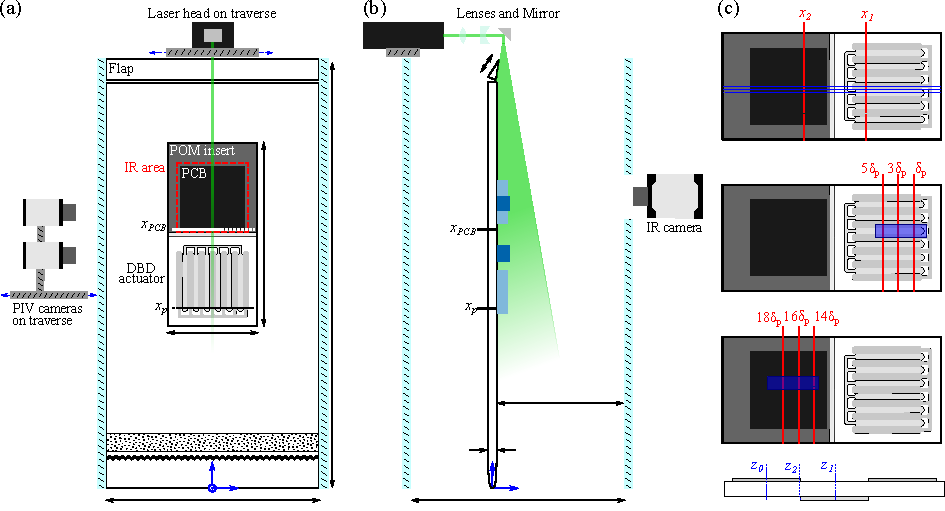
\includegraphics[width = 0.99\textwidth]{figures/methodology/setup_all_rebut.pdf}
    \caption{Schematic of the experimental setup and measuring stations. The coordinate system origin is set at the leading edge. Actuation begins at $x_p = 421\mathrm{mm}$. (a) Front view; the measurement area of infrared thermography is indicated \lcap{--}{red}. (b) Side view.; the field of view of the planar-PIV \sy{blue2}{rec} and stereo-PIV \sy{blue6}{rec} measurements are highlighted. (c) From top to bottom: streamwise \lcap{--}{red} and spanwise \lcap{--}{blue} station in planar-PIV measurements ($x_1=530\mathrm{mm}$, $x_2=675\mathrm{mm}$); region of measurement \sy{blue}{rec} and selected $\hat{x}$-planes \lcap{--}{red} for stereo-PIV; spanwise stations \lcap{--}{blue} over the cross-section of a couple of electrodes ($z_2=-6.5\mathrm{mm}$, $z_1=-13\mathrm{mm}$, $z_0=0$).}
    \label{fig:setup}
\end{figure}

The turbulent boundary layer develops on a machined aluminum flat plate  (surface roughness $R_q: 0.05\mathrm{mm}$) of $1\mathrm{m}$ length and $20\mathrm{mm}$ thickness, spanning the entire width of the test section (see figure \ref{fig:setup}). Two parallel side walls ensure two-dimensional flow while two extra walls are mounted parallel to the flat plate model, closing the test section, thus approximating zero-pressure-gradient conditions on the model. To measure the pressure distribution, the flat plate is equipped with $81$ static pressure taps spaced by $15\mathrm{mm}$ in the streamwise direction. The plate is equipped with plasma actuators and with a convective heat transfer sensor, both flush-mounted by means of polyoxymethylene (POM) inserts.

The flat plate leading edge follows a modified super-ellipse \citep{Lin1992LEeffect} to reduce curvature discontinuities. The leading edge stagnation point is controlled by a $50\mathrm{mm}$ long adjustable trailing-edge flap, deflected by approximately $15^\circ$. The boundary layer is tripped close to the leading edge with zig-zag turbulators of $1.9\mathrm{mm}$ height located at $x = 0.06\mathrm{m}$. The turbulators are followed by a $50\mathrm{mm}$ wide strip of silicon carbide grit with a characteristic height of $1\mathrm{mm}$, guaranteeing a random distribution of surface irregularities to eliminate coherent structures from the zig-zag turbulator. Care is taken to ensure that the turbulent boundary layer at the measurement locations is not affected by tripping effects \citep{sanmiguel2017diagnostic}.

%-----------------------------------------------------------------------------
%%%%%%%%%%%%%%%%%%%%%%%%%%%% PLASMA ACTUATOR  %%%%%%%%%%%%%%%%%%%%%%%%%%%%%%%%
\subsection{DBD-Plasma Actuator configuration \label{ss:PlasmaActuator}}
%-----------------------------------------------------------------------------
The DBD-plasma actuator layout is shown in figure~\ref{fig:3D_PA_detail}. The actuator assembly consists of a repeated pattern of 6 linear bi-directional actuators with spanwise wavelength $\lambda = 26 \mathrm{mm}$ and streamwise length $L = 128 \mathrm{mm}$. The electrodes are aligned parallel to the oncoming flow. Each actuator makes use of two air-exposed electrodes and one covered electrode. Neighbouring actuators make use of common exposed electrodes as well, which yields the formation of plasma on both sides of each exposed electrode. As shown later, the resulting body force distribution produces a sequence of opposing wall jets tangent to the surface in the spanwise direction which interacts with the external flow, eventually generating pairs of counter-rotating streamwise vortices with size $O(\lambda/2)$. This plasma-induced motion enhances the cross-stream mixing of momentum within the TBL, serving as the basic mechanism for flow control. The electrode array shown in figure~\ref{fig:3D_PA_detail} differs from the single streamwise-oriented DBD-actuator investigated by \citet{jukes2013plasmaVG}; however, it is very similar, both in shape and characteristics, to the Plasma Streamwise Vortex Generator (PSGV) proposed by \citet{Wicks2015} to generate streamwise vorticity within a TBL and to the Configurations A and B proposed by \citet{cheng_wong_hussain_schroder_zhou_2021} to reduce skin-friction drag within a TBL over a flat plate. The readers are referred to \citet{Kelley2016} for further insights on the design and scaling of plasma vortex generators.
%-------------------------------------------------------------------------------
\begin{figure}[t]
    \centering
    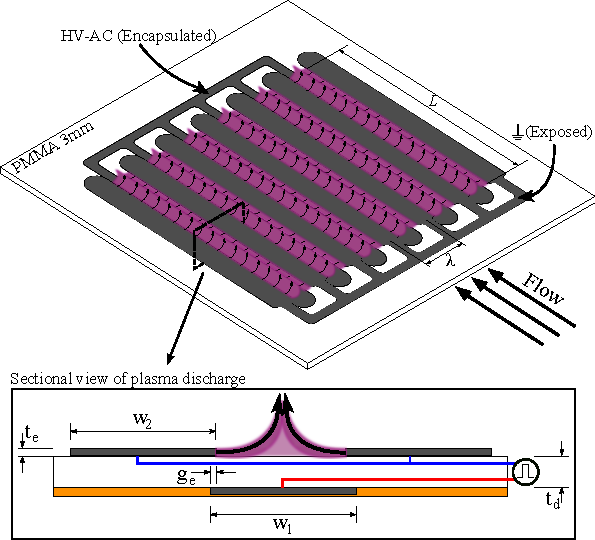
\includegraphics[width = 0.65\linewidth]{figures/methodology/3D_PA_detail_v3.pdf}
    \caption{DBD-plasma actuator array schematic. Geometrical parameters are defined in the detailed view of the DBD-plasma actuator section. The interspersed array of encapsulated and exposed electrodes \sy{electrode}{rec} is depicted. The plasma glow discharge is outlined \sy{plasma}{rec} and the polyamide insulation is highlighted \sy{kapton}{rec} for clearness.}  \label{fig:3D_PA_detail}
\end{figure}
%-------------------------------------------------------------------------------

The electrodes are manufactured using deposition of conductive silver particles in a 2-butanone solution, allowing for thin, smooth electrodes of negligible roughness $(< 10 \upmu \mathrm{m})$. Unlike previous studies using a thin dielectric barrier for streamwise-oriented actuators in laminar boundary layers \citep{Jukes2012,jukes2013plasmaVG}, control of separation in airfoils \citep{jukes2013nacaVG}, promotion of spanwise-travelling waves within a TBL \citep{Whalley2014} or streamwise-vortex generators \citep{cheng_wong_hussain_schroder_zhou_2021}, this study follows the recommendations from the work by \citet{thomas2009dbdopt}, who demonstrated a better than an order-of-magnitude increase in the plasma-induced body force produced by actuators for thicker dielectric barriers. Consequently, the arrays of exposed and covered electrodes are separated by a dielectric material (PMMA) of $3 \mathrm{mm}$ thickness (similar to the quartz dielectric used by \citet{Wicks2015} and $\approx 13$ times thicker than in \citet{Jukes2012,jukes2013plasmaVG, Whalley2014,cheng_wong_hussain_schroder_zhou_2021}. Degradation of plasma actuators, when subjected to high voltage for a long time, has been recently reported by \citet{cheng_wong_hussain_schroder_zhou_2021}. The choice of the dielectric material does not only affect the intensity of the actuation but also the robustness of the device as well as the heat generation. The plasma actuator hereby described is capable of reliably operating for long periods without loss of effectiveness, allowing the use of a single actuator array for the whole experimental campaign. Moreover, despite the fact that thicker dielectrics tend to promote higher gas heating \citep{Rodrigues2018b}, it was ensured that the actuator does not provide sufficient thermal footprint that could affect the convective heat transfer measurements.

The actuator assembly is installed on an insert manufactured with the same dielectric material. The assembly allows for a flush-mounted design in the aluminium flat plate, largely minimising surface protrusions or irregularities that can affect the developing flow. Furthermore, polyimide (Kapton) tape is used to insulate the covered electrode and the edges of the actuator plate in order to avoid spurious plasma discharges. Details on the geometrical and material properties of the plasma actuator are listed in Table \ref{tab:actuatorparam}. The actuator array is driven by a TREK 20/20C HS high-voltage amplifier, connected to the covered electrodes, while the air-exposed electrodes are kept at ground potential. A dielectric barrier discharge of weakly-ionised air is achieved using a sinusoidal voltage signal at a frequency of $2\mathrm{kHz}$. The choice of carrier frequency is made as a compromise between power delivery limitations of the TREK amplifier and sufficient separation of hydrodynamic scales. Indeed, for the present study, the carrier frequency, scaled in wall units $f_d^+ \approx 0.1$ is significantly larger than the inverse of the convective time unit of the reference TBL, $U_\infty^+/Re_\tau$ $\approx 0.04$, %(Uinf/d99) / (utau^2/nu)
effectively rendering the action of the body force time-invariant.

%-----------------------------------------------------------------------------
\begin{table}[t]
\centering
\begin{tabular}{lll}
\toprule
% \multicolumn{2}{c}{Parameter} & Value \\ \midrule
$\lambda$ & Spanwise wavelength & 26.0 mm \\
$w_1$ & Exposed electrode width & 13.5 mm \\
$w_2$ & Covered electrode width & 13.5 mm \\
$t_d$ & Dielectric thickness & 3.0 mm \\
$g_e$ & Overlap between electrodes & $\sim$0.5 mm \\
$t_e$ & Electrode thickness & $<10$ $\mu$m \\
$l$ & Electrode length & 169.5 mm \\
$L$ & Effective plasma discharge length & 128 mm \\
$V_{pp}$ & Discharge voltage peak-to-peak & 10-20 kV \\
$f_d$ & Carrier frequency & 2 kHz \\ 
$P$ & Actuator power consumption & 150-300 W/m\\
\bottomrule
\end{tabular}
\caption{Geometrical, material and operation properties of the plasma actuator}\label{tab:actuatorparam}
\end{table}

%-----------------------------------------------------------------------------
%%%%%%%%%%%%%%%%%%%%%%%%%%%%%%%%%%% PIV  %%%%%%%%%%%%%%%%%%%%%%%%%%%%%%%%%%%%%
\subsection{Velocity measurements \label{ss:PIV}}
%-----------------------------------------------------------------------------
Velocity field measurements are performed using planar, two-component Particle Image Velocimetry (PIV) in several $x-y$ planes, i.e. parallel to the freestream and normal to the flat plate, as shown schematically in figure \ref{fig:setup}. Anticipating the strongly three-dimensional nature of the flow emerging from the actuation, additional stereoscopic PIV measurements are performed for selected actuation cases.

Seeding particles are produced by a SAFEX fog generator using a glycol-water solution with a mean droplet diameter of $1 \mu\mathrm{m}$ released in the wind tunnel circuit downstream of the test section. Illumination is provided by a dual cavity Nd:Yag Quantel Evergreen laser ($200\mathrm{mJ/pulse}$ at $15\mathrm{Hz}$) and a set of cylindrical and spherical lenses. The laser sheet thickness is approximately $1\mathrm{mm}$ for the planar-PIV cases and $3\mathrm{mm}$ for the stereo-PIV. 
Two LaVision Imager sCMOS CLHS cameras are used to image the flow. Three camera configurations are composed for planar (C1 and C2) and stereoscopic (C3) measurements, shown as shaded regions in figure \ref{fig:setup}. In configuration C1, the camera fields of view (FOV) are stitched in order to obtain a combined FOV of $190\times30 \mathrm{mm}^2$ at a magnification ratio of approximately 0.16, thus, allowing to obtain an overview of the global TBL development. In turn, C2 is used to obtain high-resolution measurements for extracting TBL statistics simultaneously at two different streamwise locations (see figure~\ref{fig:setup}), with each camera having a FOV of $45\times20 \mathrm{mm}^2$ and magnification ratio of 0.37. Finally, for the stereoscopic configuration C3, the FOV is $100\times20 \mathrm{mm}^2$ at a magnification of approximately 0.16. The total measurement area by PIV spans between $0.4m\leq x \leq 0.7m$, which covers the region of interest from the upstream edge of plasma actuation to the heat-flux sensor.
%------------------------------------------------------------------------------
\begin{table}
\centering
\begin{tabular}{lccc}
% \begin{tabular}{\tblwidth}{p{0.462\linewidth-2\tabcolsep} %@{}lcc@{}}
%                 >{\centering\arraybackslash}p{0.1793\linewidth-2\tabcolsep}
%                 >{\centering\arraybackslash}p{0.1793\linewidth-\tabcolsep}
%                 >{\centering\arraybackslash}p{0.1793\linewidth-2\tabcolsep}}
\toprule
\multicolumn{1}{l}{Parameter} & C1 & C2 & C3 \\ \midrule
Camera & \multicolumn{3}{c}{LaVision’s Imager sCMOS CLHS} \\
Sensor resolution & \multicolumn{3}{c}{2560$\times$2160 px$^2$} \\
Pixel pitch & \multicolumn{3}{c}{$6.5\mu$m} \\
PIV measurement type & Planar & Planar & Stereoscopic\\
Lens focal length [mm] & 60 & 105 & 60\\
Aperture $(f_{\#})$ & 5.6 & 5.6 & 8\\
Frame separation $(\Delta t)$ [$\mu$s] & $40$ & $20$ & $40$\\
Field of view (FOV) [mm$^2$] & $190 \times 30$ & $45 \times 20$ & $100 \times 20$\\
Digital resolution [px/mm] & 25.16 & 58.41 & 25.6 \\
Magnification factor & 0.16 & 0.37 & 0.16\\
Interrogation window [px$^2$] & 12$\times$12 & 12$\times$12 & 12$\times$12 \\
Overlap factor & 50\% & 50\% & 50\%\\
Vectors per velocity field & $791\times125$ & $450 \times 200$ & $434 \times 86$\\
Vector pitch [mm] & 0.24 & 0.10 & 0.23\\
\bottomrule
\end{tabular}
\caption{PIV parameters} \label{tab:PIVparam}
\end{table}
%------------------------------------------------------------------------------

For all camera configurations and actuation conditions, an ensemble of 1300 image pairs is acquired at a sampling frequency of 15Hz. Processing of the images is carried out using LaVision DaVis 10.1 software. A multi-pass %\citep{soria1996piv} 
cross-correlation algorithm \citep{Willert1991digitalpiv} with window deformation \citep{scarano2001iterativeimgdef} is applied to the sequence of images, with a final interrogation window size of $12\times12$ $\mathrm{pixels}^2$ and 50\% of overlap. Spurious vectors are discarded by applying a universal outlier detector \citep{westerweel2005outlier} and are replaced by interpolation based on adjacent data. A summary of the relevant PIV parameters is provided in table \ref{tab:PIVparam}. The convergence of first- and second-order statistics within a variation of 1.5\% has been confirmed for all cases.

In order to capture the three-dimensional flow features emerging from the operation of the plasma actuator array, the PIV system, including cameras and laser head, is mounted on an automated traverse system allowing precise scans in the spanwise direction. For the planar-PIV cases, five planes are measured: $z_0$, $z_1$, and $z_2$ as shown in figure~\ref{fig:setup}(c), as well as the symmetric planes of $z_1$ and $z_2$ with respect to $z_0$. A more refined scanning is performed for the stereo-PIV measurements, with a total of $18$ planes, equally spaced between $z=0$ and $z=25.5\;\mathrm{mm}$ as highlighted in figure~\ref{fig:setup}(c), allowing to obtain a fully reconstructed three-dimensional mean flow.

The experimental uncertainties associated with the PIV measurements are computed from the uncertainty estimation tool developed by \citet{Castellanos2021PIVuncertainty} for PIV/EPTV measurements. The uncertainty on the TBL parameter estimation is directly related to the averaging-window size in wall units. For the PIV configuration C2, the final interrogation window corresponds to a size of 12$l^*$ (where $l^* = \nu/u_\tau$ is the viscous length), which guarantees a high-resolution measurement for the estimation of TBL parameters. Hence, the uncertainty on the integral lengths $\delta^*$ and $\theta$ and the boundary-layer thickness $\delta$ is estimated to be below $\pm 2\%$. The uncertainty for the estimation of $U_\infty$ and $u_\tau$ is well below 1\% and the position of the wall is estimated with an error below $\Delta y^+ = \pm 5$. Note that the boundary-layer thickness $\delta$ is approximated in this study as $\delta \approx \delta_{99}$, such that $u(y=\delta_{99})=0.99U_\infty$.
% Remember that my WallUnit = ~2.8e-05 m

%------------------------------------------------------------------------------
%%%%%%%%%%%%%%%%%%%%%%%%%%%%%%%%%%%% IR %%%%%%%%%%%%%%%%%%%%%%%%%%%%%%%%%%%%%%%
\subsection{Infrared thermography measurements \label{ss:IR}}

Wall heat fluxes are assessed from convective heat transfer measurements, using infrared thermography. Measuring surface heat fluxes in thermo-fluid dynamics requires both heat-flux sensors and temperature transducers. In the present work, the temperature transducer is infrared thermography, in conjunction with a heated-thin-foil sensor, a common choice in heat transfer investigations \citep{astarita2012infrared}. The chosen heat-flux sensor in this study is fabricated as a Printed Circuit Board (PCB). A PCB similar to those used in \citet{torre2018HTF} is chemically bonded to a machined insert made of POM and flush-mounted into the flat plate. The PCB features a copper track with a thickness of $5\mathrm{\mu m}$, a pitch of 2 $\mathrm{mm}$ and a gap of 0.2 $\mathrm{mm}$. The heat-flux sensor can be considered isothermal across its thickness \citep{astarita2012infrared} since the Biot number ($\mathrm{Bi} = h t/k$, where $h$ is the convective heat transfer coefficient while $k$ and $t$ represent the foil thermal conductivity coefficient and thickness, respectively) is relatively small for the proposed problem $( \mathrm{Bi} \approx 0.003)$. The heat-flux sensor is placed at a distance of $0.6\mathrm{m}$ downstream of the leading edge, i.e. $50\mathrm{mm}$ downstream of the end of the plasma discharge. 

The PCB electrode has a nominal resistance of $25.5\Omega$, a circuit area $(A_{\mathrm{PCB}})$ of $150\times 150\mathrm{mm}^2$ and a thickness of $0.5\mathrm{mm}$. A constant heat-flux $q''_{j}$ is achieved using Joule heating enabled by a stabilised power supply connected to the PCB, which provides constant voltage $V$ and current $I$ ($q''_{j} = V I / A_{\mathrm{PCB}}$). The convective heat transfer coefficient distribution is expressed in non-dimensional form in terms of Stanton number ($St = h/(\rho_{\mathrm{air}}U_\infty C_{p_{\mathrm{air}}})$), where $\rho_{\mathrm{air}}$ is the air density, $U_\infty$ is the freestream velocity, $C_{p_{\mathrm{air}}}$ is the specific heat capacity of air. The computation of $h$ is performed through a steady-state energy balance, modeling the PCB as a heated-thin-foil sensor \citep{astarita2012infrared}, %------------------------------------------------------------------------------
\begin{equation}
	h = \frac{ q''_{j} - q''_{r} - q''_{k} }{ T_{w} - T_{aw} } ,
	\label{eq:heatedthinfoil}
\end{equation}
%------------------------------------------------------------------------------
where $T_{w}$ is the surface temperature of the PCB, $T_{aw}$ is the adiabatic wall temperature, $q''_{r}$ is the radiation heat flux and $q''_{k}$ is the tangential conduction heat flux through the PCB. Heat-flux losses due to natural convection on the rear side of the PCB are minimised with a $2 \mathrm{mm}$ air gap between the rear surface of the PCB and the POM-insert. These losses are estimated to be below 1\% of the convective heat transfer using correlations for natural convection into rectangular cavities \citep{bergman2011fundamentals}. Natural convection losses on the flow-facing side are neglected since $\mathrm{Gr/Re}^2<< 1$ ($\mathrm{Gr} = {g\beta_v(T_{w}-T_{aw}) L^3}/{\nu^2}$ is the Grashoff number, where $\beta_v$ is the volumetric thermal expansion coefficient and $g$ the acceleration of gravity). The radiative heat flux $q''_{r} = \sigma \varepsilon (T_w^4 - T_\infty^4)$ (where $\sigma$ is the Boltzmann constant and $\varepsilon$ is the emissivity of the PCB surface) is estimated under the assumption that the environment behaves like a blackbody with a temperature equal to that of the free stream $T_\infty$. Although the PCB copper tracks introduce an anisotropic thermal behaviour of the board, the PCB layout complies with the criteria proposed by \citet{torre2018HTF} with the tangential conduction losses through the plate being below 0.5\%, estimated according to $q''_{k} = kt \left( \frac{\partial^2T}{\partial x^2} + \frac{\partial^2T}{\partial y^2} \right)$.

The temperature measurements are performed with a CEDIP-SC7300 Titanium IR camera (320$\times$256 pixel MCT sensor and Noise Equivalent Temperature Difference (NETD)$<25\mathrm{mK}$.), capturing images at a frequency of $10\mathrm{Hz}$ with a spatial resolution of $1.6\mathrm{pixels/mm}$. To improve the accuracy of IR measurements the PCB is coated with a thin layer of high-emissivity paint ($\varepsilon = 0.95$). The value of the wall temperature ($T_w$) and the adiabatic temperature at the wall ($T_{aw}$) are computed from two different measurement runs: $T_{aw}$ is obtained as the ensemble average of 300 images acquired with $q_j''= 0$, henceforth referred to as \textit{cold} images; $T_w$ is the ensemble average of 300 images acquired with the PCB activated, referred to as \textit{hot} images. The experimental uncertainties associated with the measurements are determined through a Monte Carlo simulation \citep{minkina2009infrared}, assuming statistically uncorrelated errors and using the uncertainty values reported in table~\ref{tab:uncertainties}. The uncertainty on the local Stanton number is estimated to be $\pm 3.7\%$.

\begin{table}
\centering
\begin{tabular}{lll}
\toprule
Parameter & Uncertainty & Typical Value \\ \midrule
$T_w$ & 0.1 K & 297 [K]  \\
$T_{aw}$ & 0.2 K & 290 [K] \\
$T_\infty$ & 0.1 K & 292 [K] \\
$V$ & 0.2\% & 17 [V] \\
$I$ & 0.2\% & 0.65 [A] \\
$\varepsilon$ & 2\% & 0.95 \\
$A$ & 0.1\% & 225 [cm$^2$] \\
$C_{p_{\mathrm{air}}}$ & 1\% & 1006 [kJ/(kg K)] \\
$\rho_{\mathrm{air}}$ & 1\% & 1.224 [kg/m$^3$] \\
$U_\infty$ & 1\% & 11.8 m/s \\
$q''_k$ & 10\% & 0.6 [W/m$^2$] \\ 
\bottomrule
\end{tabular}
\caption{Uncertainty Analysis on Stanton number calculation} \label{tab:uncertainties}
\end{table}
%------------------------------------------------------------------------------
%%%%%%%%%%%%%%%%%%%%%%%%%%%%%%%%%%%% Plasma characterization %%%%%%%%%%%%%%%%%%%%%%%%%%%%%%%%%%%%%%%
\subsection{Momentum coefficient at quiescent conditions} \label{ss:plasma_char}
%
\begin{figure}
    \centering
    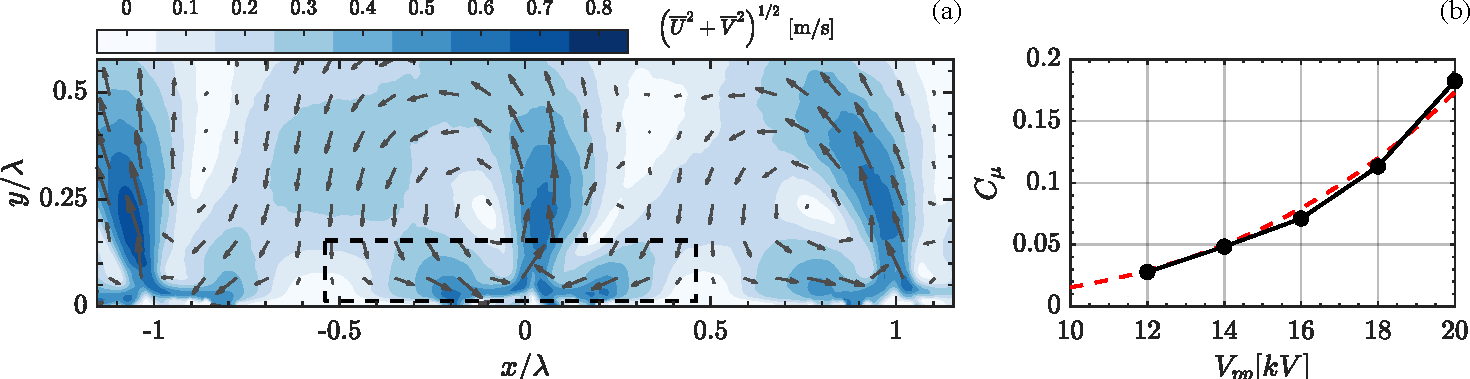
\includegraphics[width = 0.99\textwidth]{figures/methodology/plasmachar_rebut.pdf}
    \caption{Plasma characterisation. (a) Contour of the induced plasma flow velocity magnitude. The control volume for the momentum balance is highlighted \lcap{--}{black}. (b) Momentum coefficient as a function of the discharge voltage \sy{black}{o*} and experimental fit for empirical relation $C_\mu \propto V_{pp}^{7/2}$ \lcap{--}{red}} %cmu = [0 0.0153315757803183,0.0277902175268809,0.0483544971252209,0.0711091393955022,0.113346894209305,0.182458139582648];
    \label{fig:plasma_char}
\end{figure}
%
The body force produced by a DBD-plasma actuator can be directly identified as a source term in the Navier-Stokes equations, enabling the active addition of momentum to the fluid. This can be expressed in terms of momentum coefficient ($C_\mu$) \citep{Amitay2001Cmu},
\begin{equation} \label{eq:Cmu}
    C_\mu = \frac{\mathbf{\overline{I}}}{1/2\rho_\infty U_\infty^2 L}.
\end{equation}
The time-averaged momentum per unit length, $\mathbf{\overline{I}}$, is normalised by the fluid density, $\rho_\infty$, the square of the free stream velocity, $U_\infty$, and the length of the plasma actuator, $L$. In turn, $\mathbf{\overline{I}}$ is calculated as described by \citet{kotsonis2015control}, through the application of the momentum balance equation,
\begin{equation}
    \mathbf{\overline{I}} = \oint_S \rho_\infty \mathbf{\overline{u}} \left( \mathbf{\overline{u}} \cdot \mathbf{\hat{n}}  \right) \,dS,
\end{equation}
on the appropriate control volume, $S$, assuming negligible pressure contribution. Furthermore, for the conditions considered in this work, electrodynamic scales can be considered sufficiently separated from hydrodynamic scales. Consequently, the produced momentum is assumed independent of the freestream velocity \citep{Pereira2014external}, allowing quiescent conditions to be chosen for characterisation purposes. Measurements of the velocity fields at different voltage amplitudes and for continuous operation of the actuator at 2kHz carrier frequency are performed by planar-PIV in a setup dedicated to momentum coefficient quantification. The latter consists of a chamber with optical access, ensuring quiescent conditions, wherein the actuator array is placed. The chamber is filled with seeding generated by dielectric paraffin oil. Images are captured at the midspan of the electrodes $(L/2)$ over a field of view of $65\times21\mathrm{mm}^2$ and are processed to obtain velocity fields of $351\times116$ vectors at a vector pitch of 0.18mm in both directions.

A representative, time-averaged flow field of the actuator at $V_{pp} = 20\mathrm{kV}$ along with the estimated momentum coefficient for a range of peak-to-peak voltages are shown in figure~\ref{fig:plasma_char}. The actuator layout ensures a spanwise periodicity of the mean flow pattern, where the opposing jets collide and are redirected in the wall-normal direction, causing a distinct wall-normal jet whose maximum velocity is approximately 0.7 m/s at the highest discharge voltage. Since the control volume used for estimating the momentum coefficient contains the two opposing streamwise jets, the largest contribution in force originates from the momentum exchange along the $y$-direction ($C_{\mu} \approx C_{\mu_y}$), while in the $z$-direction momentum exchange is approximately zero. Characterisation is performed for a range of discharge voltages from $10\mathrm{kV_{pp}}$ to $20\mathrm{kV_{pp}}$, however, measurements at $10\mathrm{kV_{pp}}$ are not reliable. At these conditions, the induced jet velocities are very low, hence, the seeding cannot be adequately distributed in the vicinity of the actuator, causing gaps in regions relevant for estimation of the momentum coefficient. Nonetheless, through the remainder of discharge voltages, it is evident that the momentum coefficient follows the well established $7/2$th power-law, firstly proposed in \citet{Enloe2004} and later reported in numerous experiments \citep{thomas2009dbdopt,Mertz2011}.% and corke2009sdbd.
Although the $\mathrm{Re}$ number of the herein considered TBL is comparable to the one in \citet{cheng_wong_hussain_schroder_zhou_2021}, the present study is performed at a much higher freestream velocity, hence, there are higher requirements of momentum coefficient from the actuator.

%%%%%%%%%%%%%%%%%%%%%%%%%%%%%%%%%%%%%%%%%%%%%%%%%%%%%%%%%%%%%%%%%%%%%%%%%%%%%%
%%%%%%%%%%%%%%%%%%%%%%%% stereo-PIV %%%%%%%%%%%%%%%%%%%%%%%%%%%%%%%%%%%%%%%%%
%%%%%%%%%%%%%%%%%%%%%%%%%%%%%%%%%%%%%%%%%%%%%%%%%%%%%%%%%%%%%%%%%%%%%%%%%%%%%%
\section{Time-averaged flow field}\label{s:stereo}
%
\begin{figure}
         \centering
         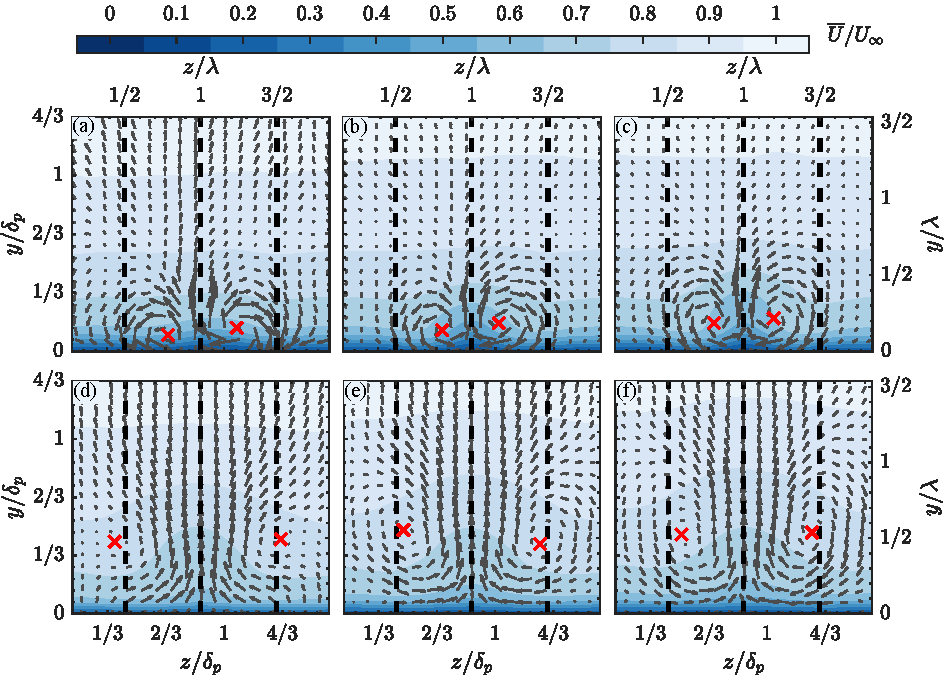
\includegraphics[width=0.99\textwidth]{figures/results/stereo/stereo_rebut.pdf}
         \caption{Evolution of plasma-induced large structures for the strongest actuation case ($V_{pp} = 20 \mathrm{kV}$, $C_\mu = 0.1825$) in the $y-z$ plane at $\hat{x} = \delta_p,~3\delta_p,~5\delta_p$ over the actuator (a-c) and $\hat{x} = 14\delta_p,~16\delta_p,~18\delta_p$ downstream of the actuation (d - f). The contour depicts the streamwise velocity distribution at each plane. The quiver represents the in-plane flow motion ($\overline{V}$,$\overline{W}$). The center of the vortex core based on $Q$-criterion is highlighted \sy{red}{x}.  From left to right, spanwise stations $z_2'$, $z_1$ and $z_2$ are highlighted \lcap{--}{black} (see figure~\ref{fig:setup}).} \label{fig:Ucont_quiver}
\end{figure}
%
As established in the previous sections, the actuator array is designed to produce strong spanwise modulations in the boundary layer, via tangential and opposing momentum addition.

The topology of the plasma-induced flow for the strongest actuation case (i.e., $V_{pp} = 20\mathrm{kV}$) is depicted in figure~\ref{fig:Ucont_quiver} for the selected locations over the flat-plate model as shown in figure~\ref{fig:setup}(c). The streamwise coordinate is defined as $\hat{x}=x-x_p$, where $x_p = 421\mathrm{mm}$ is the location of the upstream edge of the plasma discharge (being the origin located at the leading edge of the flat plate). The streamwise coordinate is normalised with the boundary-layer thickness at $x_p$, $\delta_p$, while the spanwise coordinates with the actuator wavelength $\lambda$. Figure~\ref{fig:Ucont_quiver} depicts the average streamwise velocity $\overline{U}$ on the $y-z$ plane at $\hat{x} = \delta_p,~3\delta_p,$ and $~5\delta_p$ along with a superimposed vector plot of the corresponding $\overline{V}$ and $\overline{W}$ velocity components. On the most upstream location of actuation ($\hat{x} = 0$), the fluid ejected laterally by the discharge is replenished by entertainment from above the exposed electrodes. This generates a vortical motion in the streamwise direction. The coalescence of the plasma-induced circulation with the main stream leads to twisting and folding of the spanwise vorticity at the tip of each plasma actuator. The latter causes streamwise-vortices to roll up and evolve as a partially developing starting vortex. The general evolution of this structure is similar to the observations of \citet{jukes2013plasmaVG} for a laminar boundary layer. Note, however, that the mechanism of the streamwise vortex formation differs from the creation of a starting vortex at quiescent air conditions, which is generated by the entrainment of fluid directly above the plasma region as reported by \citet{Whalley2010DBDvortex,Whalley2012startingV}. At $\hat{x} = \delta_p$, the streamwise vortices are already developed and begin to depart from the wall; their core is located at approximately $y\approx \delta_p/10$. The counter-rotating, streamwise vortices collide at $z_1$ leading to a strong upwash motion while the suction effect above the exposed electrodes keeps bringing air towards the wall at $z_2$. While the streamwise vortices develop in a region which coincides with the actuator, they are continuously strengthened, being displaced out of the wall by mutual induction \citep{Jukes2012}. The intensity of the vortices is mainly raised by the continuous momentum injection promoted by the DBD-actuator, although their interaction may exacerbate such effect \citep{Logdberg2009}. According to \citet{Pauley1988,Pauley1994}, the image vortices \citep{Ersoy1985} cause the pair of counter-rotating vortices with common upflow to move towards each other until they come to close proximity where the effect of their images cancel out. Subsequently, the vortices convect away from the wall.

The ejection of fluid normal and away from the wall at the plain of symmetry between counter-rotating vortices has been recently exploited in \citet{cheng_wong_hussain_schroder_zhou_2021} to control the turbulence regeneration mechanism within a TBL with a similar plasma-actuator array. Additionally, the pair of counter-rotating, streamwise vortices is confined in the space between two consecutive, opposing, exposed electrodes, i.e. $1/2<z/\lambda<3/2$ according to figure~\ref{fig:Ucont_quiver}, suggesting vortex stationarity.
The stationarity of the vortices in the present study has been confirmed with Proper Orthogonal Decomposition (POD) \citep{Lumley1967} during preliminary assessments on both planar- and stereo-PIV data, confirming the absence of any long-wavelength flapping modes. 

While the effect of the actuator is evident in streamwise locations where the discharge is active, it is striking to monitor the evolution of the flow field further downstream, up to $x_p\approx 20\delta_p$ (figure \ref{fig:Ucont_quiver} d-f). Although these locations are well downstream of the end of the discharge region, the effect of the actuation is still persisting. The induced structures are strong enough to divert the flow even $18\delta_p$ downstream of the plasma onset. At this streamwise location, the perturbation starts affecting also the outer region of the boundary layer via a lift-up action of the vortices towards the outer region. The region with significant spanwise velocity induced by the plasma discharge is also characterised by a low-speed streamwise velocity and is located in the gap between adjacent, opposing exposed electrodes. Nevertheless, an important consequence of the vortices interacting is their weakening along the downstream direction due to their continuous planar re-connection via cross-diffusion \citep{Hussain2011,Yao2020}. The vortices progressively expand in the spanwise direction and lose strength, in agreement with \citet{Wicks2015}. Nonetheless, the mutual interaction between the pair of vortices yields a strong wall-normal velocity that clearly persists at $\hat{x} = 14\delta_p$ and which is progressively expanded over a wider area in the spanwise direction.

\citet{Wicks2015} demonstrated that the streamwise vorticity generation is proportional to the actuator length $L$ for fixed $U_\infty$, and that the optimum inter-electrode spacing $\lambda$ is decoupled from the incoming boundary layer, being solely driven by the physics of plasma discharge. In agreement with these observations, the proposed DBD-actuator promotes strong streamwise vortices with a reminiscent and persistent effect downstream of the actuation. Moreover, the spanwise wavelength $\lambda$ is adequate to ensure the local confinement of the streamwise vortices along the electrodes.

The observed topology of the plasma-induced flow field is in agreement with the recent findings reported by \citet{cheng_wong_hussain_schroder_zhou_2021}, in which the authors conclude, from smoke-wire flow visualisation, that upon activation of control, the TBL streaks tend to merge and stabilise due to the effect of the large-scale streamwise vortices. Comparable velocity deficit has also been observed in the boundary layer with streamwise vortices induced by sub-boundary-layer vortex generators \citep{Sandborn1981}. On the other hand, high-speed fluid is trapped between the low-speed fluid ribbons due to the downwash of the streamwise vortices.

The injected momentum by the plasma actuation lifts up the near-wall flow, which eventually gives rise to streamwise vorticity, in a manner analogous to conventional vortex generators. A body force perpendicular to the freestream induces a spanwise mean velocity gradient $\partial\bar{U}/\partial z$, yielding wall-normal mean vorticity $\overline{\omega}_y$. The combination of the plasma-induced flow with the main stream causes vorticity reorientation towards the streamwise direction mainly due to the mean strain rate $\partial\bar{U}/\partial y$. Likewise, the spanwise mean vorticity in the boundary layer $\overline{\omega}_z\approx\partial\bar{U}/\partial y$ is also reoriented into the streamwise direction by the actuator-induced spanwise mean velocity gradient $\partial\bar{U}/\partial z$. This vorticity redistribution mechanism is responsible for the generation of streamwise vortices. This interaction between the boundary layer and plasma-induced body force significantly augments the production of $\overline{\omega}_x$. Since the actuator body force scales with $V_{pp}^{3.5}$ (as demonstrated in \S\ref{ss:plasma_char}), it can be concluded that the actuator-induced $\overline{\omega}_x$, and hence the intensity of the vortices, also scales with the magnitude of the body force $|F_B|$ \citep{Wicks2015}.

%%%%%%%%%%%%%%%%%%%%%%%%%%%%%%%%%%%%%%%%%%%%%%%%%%%%%%%%%%%%%%%%%%%%%%%%%%%%%%
%%%%%%%%%%%%%%%%%%%%%%%%%%%%%%% TBL  %%%%%%%%%%%%%%%%%%%%%%%%%%%%%%%%%%%%%%
%%%%%%%%%%%%%%%%%%%%%%%%%%%%%%%%%%%%%%%%%%%%%%%%%%%%%%%%%%%%%%%%%%%%%%%%%%%%%%
\section{Turbulent Boundary Layer analysis } \label{s:TBLanalysis}
%
The effect of plasma forcing on the statistical description of the boundary layer at different values of the introduced momentum coefficient is evaluated, based on the high-resolution planar-PIV measurements. The experimental study is executed for the same DBD-plasma actuator layout under a range of discharge voltages to assess the effect of the actuation depending on its relative intensity with respect to the freestream. Considering the power law governing the forcing intensity to voltage, the cases are evaluated in terms of momentum coefficient although the discharge voltage is used as the label for clearness in the figures. For conciseness, the TBL analysis is only shown for the representative cases $V_{pp} = 0,10,18,20\mathrm{kV}$, where $V_{pp}=0\mathrm{kV}$ corresponds to the reference boundary layer without actuation.

The TBL statistics and profiles are obtained at selected streamwise and spanwise locations over the flat-plate model as depicted in figure~\ref{fig:setup}(c). For the subsequent analysis, two streamwise stations are selected: $x_1 = 0.53\mathrm{m} = {x}_p + 8\delta_p$; and $x_2 = 0.65\mathrm{m} = {x}_p + 16\delta_p$. The former allows monitoring of the effect of the plasma actuation on the TBL at the actuator region, while the latter focuses on the wake, far downstream of actuation. Similarly, the selected spanwise stations (see figure~\ref{fig:setup}(c)) are: $z_1 = -\lambda/2 =-13\mathrm{mm}$, coinciding with the intersection of the two opposing plasma discharges; and $z_2 = -\lambda/4 = -6.5\mathrm{mm}$, placed 0.25mm towards the suction side of the exposed electrode. 

The results are presented in inner unit scaling, with the corresponding normalisation with the friction velocity $u_\tau$ and the kinematic viscosity $\nu$. The value of $\nu$ is adjusted for each independent profile based on Sutherland's law \citep{Sutherland1893law}, using the ambient pressure and temperature measurements of the incoming flow. The value of $u_\tau$ for the non-actuated boundary layer is obtained by fitting the composite profile proposed by \citet{chauhan2009}. Note that fitting methods, as herein utilised, cannot be used for manipulated boundary layers. The value of $u_{\tau}$ for the non-actuated configuration is, therefore, used as the reference for both the non-actuated and the plasma-actuated flow. The considered normalisation ensures that all profiles collapse in the outer region. The normalisation of the TBL profiles with the local friction velocity (not available from the experimental measurements), which is considerably altered by the action of the plasma-induced streamwise vortices, would imply a shift of the profiles. This approach is followed in \citet{cheng_wong_hussain_schroder_zhou_2021}, in which hot-wire data was available, and hence, it becomes difficult to compare results.

%-----------------------------------------------------------------------------
%%%%%%%%%%%%%%%%%%%%%%%%%%%%%%%%%%%% TBL %%%%%%%%%%%%%%%%%%%%%%%%%%%%%%%%%%%%%
\subsection{Characterisation of the reference TBL \label{ss:refTBL}}
%-----------------------------------------------------------------------------
Characterisation of the reference turbulent boundary layer begins by assessing the streamwise pressure gradient using data from pressure taps. A weak favourable pressure gradient along the flat plate is identified with pressure coefficient values of $-0.02 \leq C_\mathrm{p} \leq 0.02$ in the region of interest.
The absolute value of the Clauser pressure-gradient parameter computed for the reference TBL is below 0.003, which is considered to be sufficiently low for a representative zero-pressure-gradient (ZPG) condition with minimal effect on the statistics as demonstrated in \citet{guemes2019APG}.

For the determination of mean wall-shear stress and the corresponding friction velocity as well as for boundary-layer parameter estimation, high-resolution PIV measurements are employed (described in \S\ref{ss:PIV} as configuration C2). In this work, the composite profile by \citet{chauhan2009} is used to infer the actual wall-position and the value of the friction velocity, by fitting the experimental data up to $y^+ = 30$. The robustness of this method has been well established, provided that near-wall measurements are available \citep{orlu2010wallpos,rodriguez2015skinfric,vinuesa2016nagib}. To this end, planar, high-resolution PIV measurements allowed to obtain a sufficiently large number of points within the buffer region to correct for the absolute wall position and determine the friction velocity without relying on log-law constants.

Care is taken to ensure a well-behaved TBL in the region of interest, from $x_p$ to the downstream edge of the PCB. The mean streamwise velocity profile, $\overline{U}^+$, measured at the downstream edge of the plasma actuator ($x=x_p + L$ , $z = 0$) is shown in figure~\ref{fig:TBLref}, fitted on the composite profile by \citet{chauhan2009}. The TBL profile agrees well with \citet{jimenez2010} DNS data. The method proposed by \citet{sanmiguel2017diagnostic}, based on the diagnostic plot \citep{alfredsson2011diagnostic}, is employed to assess the convergence towards a well-behaved ZPG TBL. The diagnostic plot parameters are attached in table~\ref{tab:diagnostic}, concluding the agreement with DNS data and with the empirical correlations of the method. In addition, complementary boundary-layer parameters of the TBL without actuation are reported in table \ref{tab:TBLparams}.

\begin{figure}
    \centering
    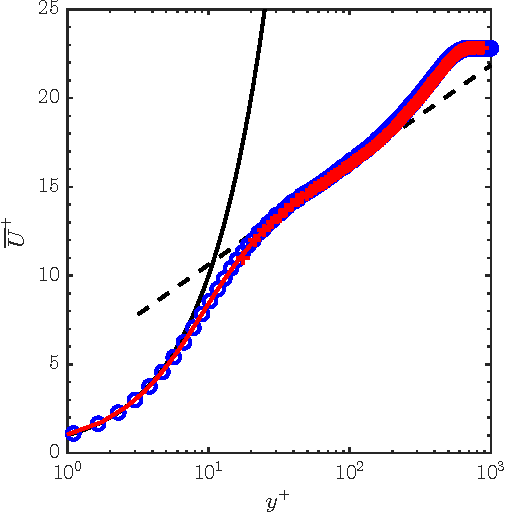
\includegraphics[width = 0.7\linewidth]{figures/methodology/TBLref.pdf}
    \caption{Profiles of the reference TBL at the downstream edge of the plasma actuator ($x=x_p+L$). PIV experimental data \sy{red}{+} is depicted together with its fit based on \citet{chauhan2009} \lcap{-}{red} and compared against DNS data from \citet{jimenez2010} \sy{blue}{o}. The viscous sublayer $U^+ = y^+$ \lcap{-}{black}, and the logarithmic law $U^+=\frac{1}{0.41} \mathrm{ln}y^+ + 5.0$ \lcap{--}{black} are included for reference.}
    \label{fig:TBLref}
\end{figure}
%----------------------------------------------------------------------------
\begin{table}
\centering
\begin{tabular}{llcc}
\toprule
Case & $Re_\theta$ & $\alpha$ & $\beta$ \\ \midrule
Reference TBL & 1596 & 0.28 ($-4.3\%$) & 0.25 ($-4.1\%$) \\
\citet{jimenez2010} & 1592 & 0.30 ($+4.1\%$) & 0.27 ($+2.5\%$) \\
\bottomrule
\end{tabular}
\caption{Diagnostic plot parameters of the reference TBL depicted in figure~\ref{fig:TBLref} and the DNS data from \citet{jimenez2010}. Error with respect to the method by \citet{sanmiguel2017diagnostic} between brackets.}\label{tab:diagnostic}
\end{table}
%----------------------------------------------------------------------------

%------------------------------------------------------------------------------
%%%%%%%%%%%%%%%%%%%%%%%%%%%%% mean-actuated TBL %%%%%%%%%%%%%%%%%%%%%%%%%%%%%
\subsection{Plasma forcing effect on the mean flow field \label{ss:meanTBL}}
%------------------------------------------------------------------------------
The $\overline{U}^+$ and $\overline{V}^+$ mean velocity profiles are shown in figure~\ref{fig:UmVmprofile} for the selected $x$ and $z$ locations. It should be noted that the results at the plane of symmetry ($z=0$) are not evaluated in this analysis as in that region the effect of the plasma actuation is negligible. Instead, the plasma forcing action is localised in the vicinity of the discharge edge of the electrode ($z_2$) and in the stagnation area where the two opposing jets collide ($z_1$). 

For the weakest forcing ($C_\mu = 0.0153$, i.e.  $V_{pp}=10\mathrm{kV}$), minimal flow distortion is observed, restricted in the near-wall region ($y^+<50$). Nevertheless, the effect of actuation intensifies with increasing momentum coefficient, while the mean flow deformation identified throughout the TBL extends from the wall to the outer region. The plasma actuator imparts two main changes to the mean flow: a suction effect at the edge of the exposed electrode, extracting fluid from the upper region of the boundary layer towards the wall and hence considerably modifying the inner region of the boundary layer, as shown in figures~\ref{fig:UmVmprofile}(b,f); and a momentum injection perpendicular to the main stream directly induced by the plasma actuator, distorting the TBL profile from the viscous sublayer up to $y^+\approx 400$ as shown in figures~\ref{fig:UmVmprofile}(a,e). These two contributions, although induced by the same actuation, promote substantially disparate effects on the TBL. Similar results have been recently reported by \citet{cheng_wong_hussain_schroder_zhou_2021}. It is to be noted, however, that the aforementioned study reports a non-monotonic increase of the actuation effectiveness with momentum injection (i.e discharge voltage). The authors claim that there exists an optimum discharge voltage for which drag reduction is maximized while further increasing the momentum injection would be detrimental since the induced vortices grow rapidly, causing an increase in vortex-induced shear stress. The present study shows a monotonic increase of the actuation effectiveness with momentum coefficient; however, discrepancies may be due to the considered discharge voltages and freestream velocity, which are up to 4 and 5 times higher in the present study, respectively. 

\begin{figure}[h!] % TBL profiles
    \centering
    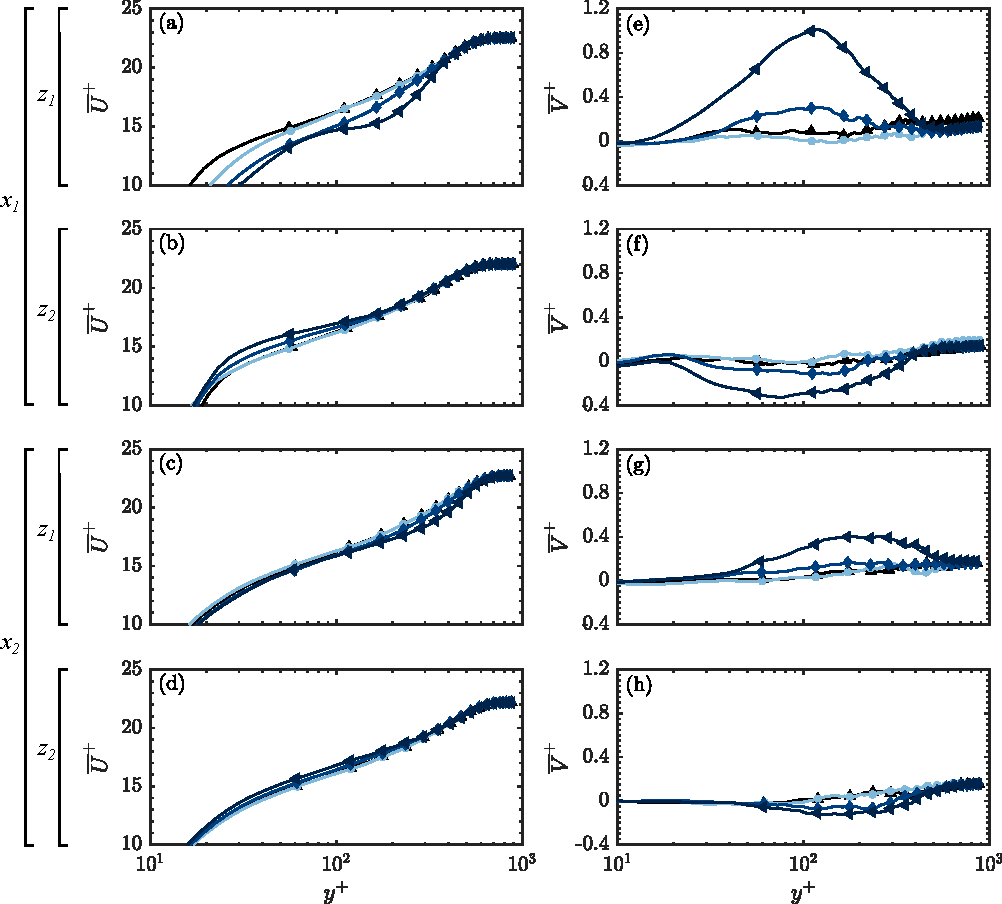
\includegraphics[width = 0.99\textwidth]{figures/results/TBL/U_V_profilesv3.pdf}
    \caption{Inner-scaled mean velocity profiles at selected stations according to figure~\ref{fig:setup}. Streamwise and wall-normal velocity profiles are depicted in the left column (a-d) and right column (e-h) respectively, for selected discharge voltages $V_{pp}=$ (and momentum coefficient $C_\mu = $) 0 \sy{black}{t*}, 10 (0.0153) \sy{blue2}{o*}, 18 (0.1133) \sy{blue6}{d*}, 20 (0.1825) \sy{blue7}{lt*}.}
    \label{fig:UmVmprofile}
\end{figure}%

From the $\overline{V}^+$ profiles, it is evident that the main perturbation on the reference flow manifests at $z_1$ for the strongest forcing case ($c_{\mu} = 0.1825$), characterised by a peak of positive wall-normal velocity at $y^+\approx 100$ in the vicinity of the actuator. This peak is a direct consequence of the opposing plasma-induced jets interacting, which eventually lift up from the wall causing a strong wall-normal motion. This effect is in agreement with the $\overline{U}^+$ profiles, in which a clear velocity deficit is induced by the forcing close to the wall.
Although the abrupt change in wall-normal velocity is only visible for the strongest forcing cases, the deficit in streamwise velocity is evident even for the weakest actuation. It can be conjectured that the changes are, therefore, limited to the inner part of the boundary layer, while for stronger actuation a larger-scale effect is observed, with the penetration of the perturbation towards the outer layer.

Downstream of the actuator ($x_2$), the dissipation of the induced motion becomes clear; however, a significant deficit of $\overline{U}^+$ is identified in figure~\ref{fig:UmVmprofile}(c), with displacements visible up to the outer region of the TBL. Analogously, the $\overline{V}^+$ peak is also progressively displaced away from the wall with a considerable reduction in magnitude (see figure~\ref{fig:UmVmprofile}g). It is evident that, while the injection of momentum in the wall-normal direction rapidly dissipates, the modification of the inner region is persistent.

The action of the plasma forcing in the suction side $z_2$
is characterised by a negative wall-normal velocity component above the wall as shown in figure~\ref{fig:UmVmprofile}(f). The flow accelerates in the streamwise direction, causing a raise in $\overline{U}^+$ slightly above the wall in the vicinity of the actuator (see figure~\ref{fig:UmVmprofile}b). The local pressure reduction, as a consequence of the suction, is responsible for the acceleration of the fluid. Both effects are strong enough to propagate downstream while displacing the local disturbances further from the wall as depicted in figures~\ref{fig:UmVmprofile}(d)~and~\ref{fig:UmVmprofile}(h).

Following the previous discussion on the effect of plasma actuation on the TBL, an analysis is performed on the evolution of $\delta$, $\delta^*$, and $\theta$. These TBL parameters for each of the evaluated cases are provided in table~\ref{tab:TBLparams}. The non-actuated TBL, highlighted in bold, is characterised by a shape factor of $H=1.46$, and a Reynolds number based on friction velocity $Re_\tau=\delta u\tau/\nu$ ranging from $582$ to $644$ between $x_1$ and $x_2$. The effect of the actuation is better understood from the variation of the parameters with respect to the non-actuated case that is within brackets. The variation of boundary-layer parameters is visualised in figure~\ref{fig:TBLstats_xz} along the streamwise and spanwise direction. The results depicted in figure~\ref{fig:TBLstats_xz}(a-c) and figure~\ref{fig:TBLstats_xz}(d-f) are computed from the stereo-PIV (C3) and planar-PIV (C1) measurements, respectively. Despite the lower resolution provided by measurement configurations C1 and C3, these results provide an overall insight of the TBL parameters distribution, with values in accordance to those reported in table~\ref{tab:TBLparams} computed from high-resolution PIV data (based on C2).

%-------
\begin{figure}
    \centering
    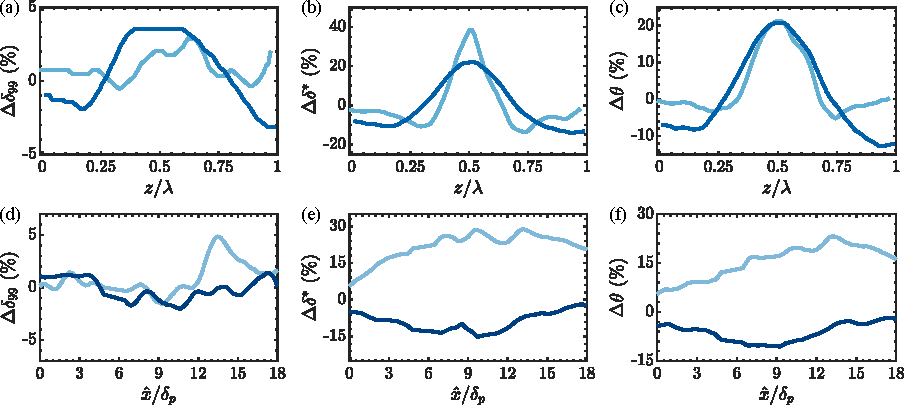
\includegraphics[width = 0.99\textwidth]{figures/results/stereo/TBLstats_xz.pdf}
    \caption{Turbulent-boundary-layer parameters for the strongest actuation case ($V_{pp} = 20 \mathrm{kV}$, $C_\mu = 0.1825$). (a-c) Distribution across the actuator wavelength ($\lambda$) at $\hat{x} = 87\mathrm{mm} \approx 6\delta_p$ \lcap{-}{blue3} and $\hat{x} = 257\mathrm{mm} \approx 18\delta_p$ \lcap{-}{blue5}; (d-e) Evolution along the streamwise direction at $z_1$ \lcap{-}{blue2} and $z_2$\lcap{-}{blue6}.}
    \label{fig:TBLstats_xz}
\end{figure}

%-------
\begin{table}
\centering
\resizebox{\textwidth}{!}{%
%\begin{tabular}{>{\centering}p{0.06\linewidth-2\tabcolsep}
%                >{\centering}p{0.06\linewidth-2\tabcolsep}
%                >{\centering}p{0.11\linewidth-2\tabcolsep}
%                >{\centering}p{0.11\linewidth-2\tabcolsep}
%                >{\centering}p{0.11\linewidth-2\tabcolsep}
%                >{\centering}p{0.11\linewidth-2\tabcolsep}
%                >{\centering}p{0.11\linewidth-2\tabcolsep}
%                >{\centering}p{0.11\linewidth-2\tabcolsep}
%                >{\centering}p{0.11\linewidth-2\tabcolsep}
%                >{\centering\arraybackslash}p{0.11\linewidth-2\tabcolsep}}
\begin{tabular}{llllllllll}
\toprule
$x_{LE}$ & $z$ & $V_{pp}$ & $C_\mu$ & \multicolumn{2}{c}{$\delta$} & \multicolumn{2}{c}{$\delta^*$} & \multicolumn{2}{c}{$\theta$} \\
 &  & $(kV)$ &  & \multicolumn{2}{c}{$(mm)$} & \multicolumn{2}{c}{$(mm)$} & \multicolumn{2}{c}{$(mm)$}\\ \midrule
\multirow{7}{*}{$x_1$} &  & \textbf{0} & \textbf{-} & \textbf{16.1} &  & \textbf{2.66} &  & \textbf{1.82} & \\
 & \multirow{3}{*}{$z_1$} & 10 & 0.0153 & 16.2 & {(+0.3\%)} & 2.75 & \green{(+3.6\%)} & 1.83 & {(+0.5\%)}\\
 &  & 18 & 0.1133 & 16.3 & {(+1.4\%)} & 3.09 & \green{(+16.4\%)} & 1.97 & \green{(+8.5\%)}\\
 &  & 20 & 0.1825 & 16.2 & {(+0.6\%)} & 3.52 & \green{(+32.5\%)} & 2.18 & \green{(+19.7\%)}\\
 & \multirow{3}{*}{$z_2$} & 10 & 0.0153 & 16.0 & {(-0.1\%)} & 2.63 & {(-0.8\%)} & 1.81 & {(-0.6\%)}\\
 &  & 18 & 0.1133 & 16.4 & {(+1.8\%)} & 2.55 & \red{(-3.9\%)} & 1.78 & \red{(-2.3\%)}\\
 &  & 20 & 0.1825 & 16.3 & {(+1.1\%)} & 2.46 & \red{(-7.4\%)} & 1.74 & \red{(-4.5\%)}\\ \midrule
\multirow{7}{*}{$x_2$} &  & \textbf{0} & \textbf{-} & \textbf{18.0} &  & \textbf{2.94} &  & \textbf{2.01} & \\
 & \multirow{3}{*}{$z_1$} & 10 & 0.0153 & 17.7 & {(-1.8\%)} & 2.91 & {(-1.0\%)} & 1.99 & {(-1.0\%)}\\
 &  & 18 & 0.1133 & 18.0 & {(-0.1\%)} & 3.13 & \green{(+6.6\%)} & 2.13 & \green{(+6.3\%)}\\
 &  & 20 & 0.1825 & 18.6 & \green{(+3.3\%)} & 3.47 & \green{(+18.1\%)} & 2.38 & \green{(+18.9\%)}\\
 & \multirow{3}{*}{$z_2$} & 10 & 0.0153 & 18.0 & {(+0.2\%)} & 3.00 & \green{(+2.1\%)} & 2.04 & {(+1.5\%)}\\
 &  & 18 & 0.1133 & 18.1 & {(+0.7\%)} & 2.85 & \red{(-3.2\%)} & 1.95 & \red{(-2.6\%)}\\
 &  & 20 & 0.1825 & 17.9 & {(-0.6\%)} & 2.76 & \red{(-6.0\%)} & 1.91 & \red{(-4.6\%)}\\ \bottomrule
\end{tabular}}
\caption{Experimental parameters of the boundary layers for the cases shown in figure~\ref{fig:UmVmprofile}. The parameters corresponding to the reference TBL are highlighted in \textbf{bold}. Relative change of the experimental parameters with respect to the reference TBL without actuation is between brackets. Positive increments above 2\% are highlighted in \green{green} and negative increments below -2\% in \red{red}.\label{tab:TBLparams}}
\end{table}
%-----

The momentum injection of plasma does not cause any significant modification of $\delta$ along either $x$ or $z$ unlike observations in previous contributions studying streamwise vortices embedded in a TBL \citep{Eibeck1987,Pauley1988,Pauley1994}. Instead, the main contribution of the plasma forcing at $z_1$ is a remarkable increase in the displacement thickness. A larger $\delta^*$ is a direct indication of higher mass flux deficit $\left(\rho\left[ U_\infty-u(y)\right]\right)$ within the boundary layer, which is also seen in the $\overline{U}^+$ profiles shown in figure~\ref{fig:UmVmprofile}(a). Analogously, the increase of momentum thickness is related to a positive increment of the deficit of momentum flux $\left(\rho u(y)\cdot\left[ U_\infty-u(y)\right]\right)$ through the boundary layer. Note, however, that the increment in $\theta$ is less pronounced than the one in $\delta^*$ since the momentum flux deficit is affecting layers where $u$ is small, i.e. in the inner region, thus determining an increase of the shape factor $H$. 

Far downstream from the actuation at $x_2$ ($\hat{x}\approx 16$), the TBL is still reminiscent from the induced vortical motion by the plasma actuator; however, the inner region of the TBL progressively adapts to the new flat-plate, smooth-surface condition, and, hence, the fluid blockage induced by plasma forcing at $z_1$ upstream is considerably reduced as suggested by the $\delta^*$ values. Conversely, the reduction of $\delta^*$ and $\theta$ for $z_2$ is a direct indicator of a reduction in mass- and momentum-flux deficits respectively. 

%%%%%%%%%%%%%%%%%%%%%%%%%%%%%%%%%%%%%%%%%%%%%%%%%% Fluctuations %%%%%%%%%%%%%%%%%%%%%%%%%%%%%%%%%%%%%%%%%%%%
\subsection{Actuation effect on the fluctuating flow field}
The normal streamwise $\overline{u^2}^+$, wall-normal $\overline{v^2}^+$ and premultiplied turbulence production profiles in inner units are reported in figure~\ref{fig:u2v2Pprofile}. Turbulence production is expressed by:
\begin{equation}
    P = -\overline{u_i u_j}\overline{S_{ij}}, \qquad \overline{S_{ij}} = \left( \frac{\partial U_i}{\partial x_j} + \frac{\partial U_j}{\partial x_i} \right),
     \label{eq:TurbProdFull}
\end{equation}
where $u_i$ is the fluctuating $i^{th}$ velocity component, $\overline{S_{ij}}$ is the strain rate tensor and $U_i$ is the $i^{th}$ mean velocity component. %\citep{pope2000}. 
An order-of-magnitude analysis based on stereo-PIV dataset confirms that the dominant component of the turbulence production is $-\overline{uv}\overline{S_{xy}}$. The turbulence production scaled in inner variables $P^+$ can thus be written as
\begin{equation}
    P^+ \approx -\overline{uv}^+ \frac{\partial U^+}{\partial y^+}. \label{eq:TurbProdRed}
\end{equation} 
%
\begin{figure} % TBL profiles
    \centering
    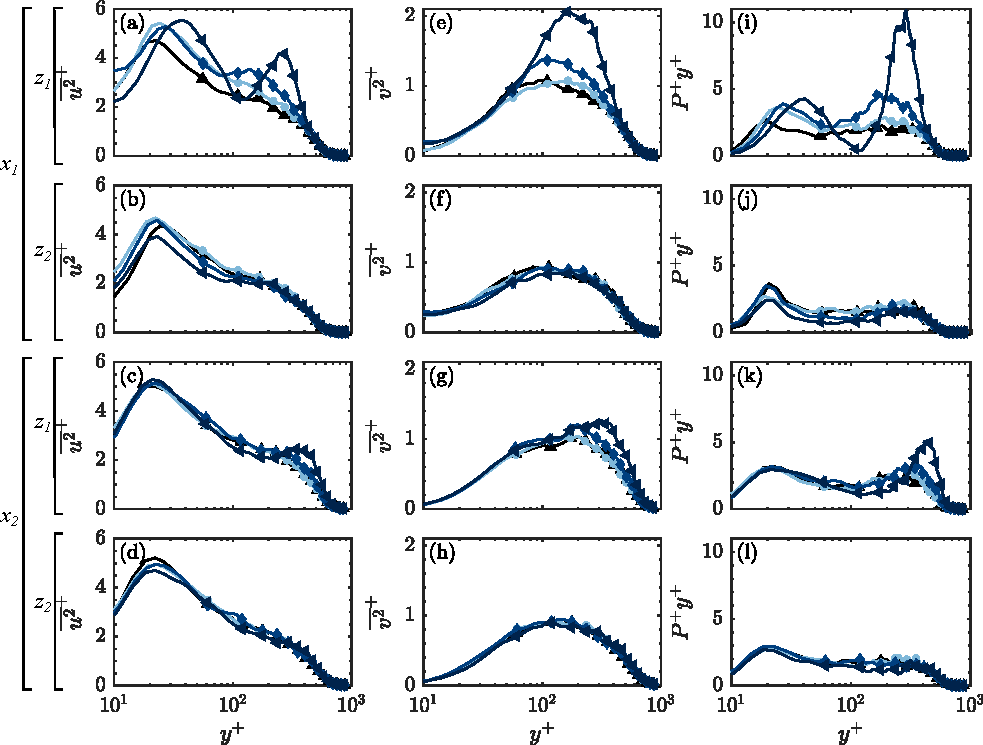
\includegraphics[width = 0.99\textwidth]{figures/results/TBL/u2_v2_P_profilesv2}
        \caption{Inner-scaled fluctuating velocities at selected stations according to figure~\ref{fig:setup}. $\overline{u^2}^+$, $\overline{v^2}^+$ and $P^+y^+$ profiles are depicted in the left column (a-d), center column (e-h) and right column (i-l) respectively, for selected discharge voltages $V_{pp}=$ (and momentum coefficient $C_\mu = $) 0 \sy{black}{t*}, 10 (0.0153) \sy{blue2}{o*}, 18 (0.1133) \sy{blue6}{d*}, 20 (0.1825) \sy{blue7}{lt*}.}
    \label{fig:u2v2Pprofile}
\end{figure}%
Focusing on the spanwise station $z_1$, there is a clear effect of the induced jets on the position and intensity of the inner peak of $\overline{u^2}^+$, and on the turbulent fluctuations in the outer layer. The inner peak is displaced away from the wall, while an outer peak is produced at the outer layer. The latter effect becomes evident for increased forcing. Moreover, the $\overline{u^2}^+$ profile exhibits a valley between both peaks, which becomes more pronounced with increasing amplitude of actuation. An outer peak is also observed in the profile of $\overline{v^2}^+$. The shape of the profiles depicted in figure~\ref{fig:u2v2Pprofile}(a) is likely due to enhanced large-scale motions.
The displacement of the inner peak in $\overline{u^2}^+$ can be ascribed to the mutual interaction between wall-tangent plasma jets which are lifted away from the wall as the forcing becomes stronger. The outer peak in $\overline{u^2}^+$ corresponds to the wall-normal location of the onset of the streamwise vortices. This is in accordance with the pronounced reduction between the inner and the outer peak, where there is a considerable component of wall-normal velocity induced by the vortex interaction as described for the mean-fields in figure~\ref{fig:UmVmprofile}(e). Moreover, the profiles of $\overline{v^2}^+$ show a peak that coincides with the valley in $\overline{u^2}^+$, at the region where the pair of counter-rotating vortices couple to promote a wall-normal motion. The values of $\overline{u^2}^+$, $\overline{v^2}^+$ at $z_2$ are almost unaltered with respect to the reference TBL as shown in figure~\ref{fig:u2v2Pprofile}. Therefore, plasma forcing is mainly affecting the mean-field in the vicinity of $z_2$ while it is very effective in manipulating both fluctuating and mean-field for the plasma side where the opposing plasma jets collide and generate wall-normal motion $(z_1)$. Focusing on the downstream persistence of the actuation, figure~\ref{fig:u2v2Pprofile}(c,g) show how both $\overline{u^2}^+$ and $\overline{v^2}^+$ rapidly adjust to the new wall condition without actuation within the wall region. On the other hand, the perturbation of the outer layer is more persistent, as presented in the form of a localised increase in $\overline{u^2}^+$ and $\overline{v^2}^+$ at $y^+\approx 400$ and $y^+\approx 300$ respectively.

The inner-scaled turbulence production in the premultiplied form $P^+y^+$ (calculated from equation~\ref{eq:TurbProdRed}) is preferred since, when represented in semi-logarithmic form, equal areas correspond to equal contributions to the production \citep{Marusic2010wbt}. ZPG TBLs are characterised by a relatively flat $P^+y^+$ distribution as shown for $V_{pp} = 0 kV$ case in figure~\ref{fig:u2v2Pprofile}(i-l). In the case of plasma actuation, the effect at $z_1$ presents some analogies with that observed in APG TBLs, with a production peak in the outer layer \citep{harun2013pressure,bradshaw1967}. Interestingly, the position of the production peak at $z_1$ coincides with the peak in the $\overline{uv}$, meaning that the main effect of the plasma actuation is to change the distribution of energy through the boundary layer, displacing large energetic structures from the near-wall region to the outer region. Although the DBD-actuator increases $\delta^*$ and $\theta$, and forces the flow in the wall-normal direction, the value of $\delta$ is almost unaffected. Hence, as the effect of the actuation is displaced downstream and for the strongest forcing, the production peak is shifted toward higher $y^+$. In contrast, at the spanwise station $z_2$, the effect on $P^+y^+$ exhibits a distribution that resembles that of a ZPG-TBL or even an FPG-TBL. However, for the streamwise station closer to the actuator ($x_1$), the plasma-induced jets seem to effectively reduce the turbulence production within the logarithmic layer with respect to the non-actuated case. Such an opposite phenomenon is in accordance with the reduction of displacement and momentum thickness of the TBL and the suction motion induced by the discharge, which eventually displaces the fluid in the logarithmic and outer region of the TBL towards the wall.

It becomes evident that the plasma induces spanwise and wall-normal motions in the near-wall layer. The peak in $\overline{v^2}^+$ occurs at $y^+= 110$, whilst $P^+y^+$ has two peaks, occurring at $y^+ = 40$ and $y^+ = 120$. One can interpret these mean locations as the bottom, centre, and top of the plasma-induced streamwise vortices. The peak in $\overline{v^2}^+$ closely corresponds to the position of the average height of the plasma-induced streamwise vortex cores due to the low momentum fluid entrained within them, and due to wall-normal induced vortex motions to either side of the core. The first peak of $P^+y^+$ marks the lower extent of the plasma vortices due to spanwise induced vortex motions below the core, and also corresponds to the location of the maximum $\overline{u^2}^+$. The second peak of $P^+y^+$ corresponds to the upper extent of the vortices and also coincides with the location of the second $\overline{u^2}^+$ peak. 

A final comment can be made on the phenomena described by the turbulence intensity downstream of the actuation. In figures~\ref{fig:u2v2Pprofile}(k,l), it is observed that the smaller energetic scales in the buffer region are already adjusted to the new wall condition. Conversely, the large-scale motions, which are over-energised (relative to the new smooth-wall boundary condition), retain a strong footprint within the boundary layer, extending deep into the buffer region. Similar results were achieved by \citet{jukes2006TBLcontrol} with a 40\% reduction in mean streamwise velocity and a 30\% reduction in turbulent intensity observed for $y^+< 30$.

%%%%%%%%%%%%%%%%%%%%%%%%%%%%%%%%%%%%%%%%%%%%%%%%%%%%%%%%%%%%%%%%%%%%%%%%%%%%%%
%%%%%%%%%%%%%%%%%%%%%%%%% Stanton number measurements %%%%%%%%%%%%%%%%%%%%%%%%
%%%%%%%%%%%%%%%%%%%%%%%%%%%%%%%%%%%%%%%%%%%%%%%%%%%%%%%%%%%%%%%%%%%%%%%%%%%%%%
\section{Wall distribution of the Stanton number}\label{s:resultsSF}
%---
\begin{figure}[h]
         \centering
         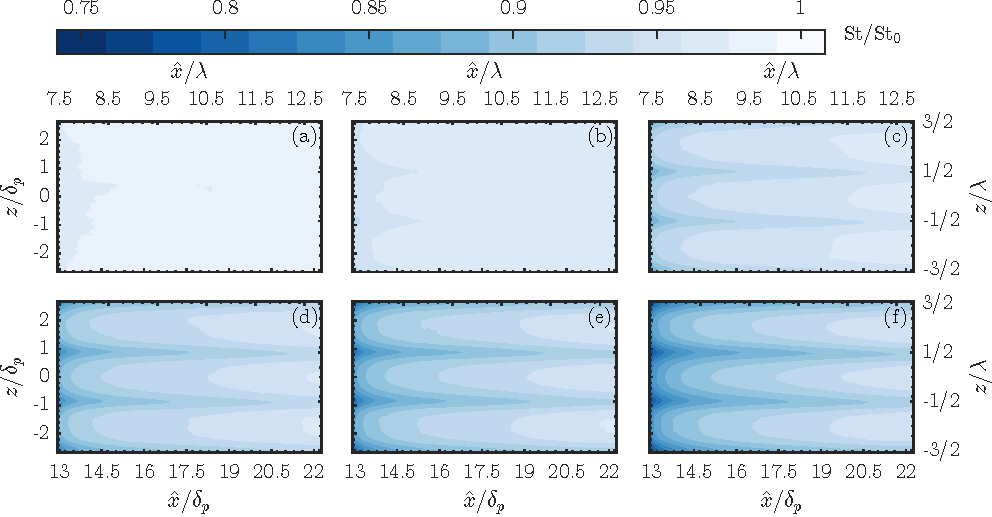
\includegraphics[width=0.99\linewidth]{figures/results/St/st_rebut.pdf}
         \caption{$\mathrm{St}(x,z)/\mathrm{St_0}(x,z)$ distribution on the region of interest for the tested discharge voltages $V_{pp}=$  (and momentum coefficient $C_\mu = $) 10 (0.0153) (a), 12 (0.0278) (b), 14 (0.0484) (c), 16 (0.0711) (d), 18 (0.1133) (e), 20 (0.1825) (f).} \label{fig:st_maps} % [0 0.0153,0.0278,0.0484,0.0711,0.1133,0.1825]
\end{figure}
%---
Infrared thermography measurements with a PCB as a heat-flux sensor are carried out to understand whether the persistent perturbation in the outer layer by the plasma actuation has a corresponding footprint on the convective heat transfer at the wall. Based on the conclusion that the plasma momentum injection, perpendicular to the main stream, triggers the formation of pairs of counter-rotating vortices, the calculation of the Stanton number at the wall aims at corroborating the behaviour of such large-scale motion and its persistence in the far-field downstream of the actuation. 
The time-averaged Stanton number distributions on the wall downstream of the control region for the different plasma discharge voltages are shown in figure~\ref{fig:st_maps}. The results are normalised with the wall-distribution of Stanton number at non-actuated flow conditions $\mathrm{St}_0$. A region of interest is considered, covering two pairs of DBD-actuators in the spanwise direction (approximately 1.5$\lambda$ at each side of the symmetric, $xy$-plane) and a considerable range in the streamwise direction of $13\leq\hat{x}/\delta_p\leq 22.5$. Note that the IR images are taken at a distance of 13$\delta$ from $x_p$, which implies a physical distance of $185\mathrm{mm}$ from the upstream edge of the plasma discharge and $55\mathrm{mm}$ from its downstream edge.  

Analysing the weakest plasma forcing configuration in figure~\ref{fig:st_maps}(a), it is clear that the actuation tends to uniformly reduce the Stanton number for the whole region of interest. As the discharge voltage is increased, a localised, more significant $\mathrm{St}$ reduction is evident at the location where plasma jets oppose each other. Therefore, the plasma forcing is composed of two main effects on the Stanton number distribution: a uniform reduction, and a localised decrease at the location where the plasma-induced jets lift-off. The first contribution can be understood as a consequence of the increased momentum defect in the inner region, which thus results in reduced heat transfer. On the contrary, the second effect promotes the streak-like pattern identified at $z/\lambda \approx \pm 1/2$. The superposition of both contributions becomes evident when computing the normalised, streamwise average over the region of interest $\langle \mathrm{St} \rangle$, shown in figure~\ref{fig:meanSt_delta}(a),
\begin{equation}
    	\langle \mathrm{St} \rangle = \int \mathrm{St}(x,z) \,\mathrm{d}x .
\end{equation}
The uniform reduction in convective heat transfer at the wall grows with the intensity of the actuation, corroborating the monotonic increase in actuation effectiveness with $C_\mu$ as previously reported from the TBL profiles. Similarly, the irregular actuation generating the streak-like pattern also intensifies, causing higher amplitudes in the oscillation along with the spanwise component.  
%----
\begin{figure}
         \centering
         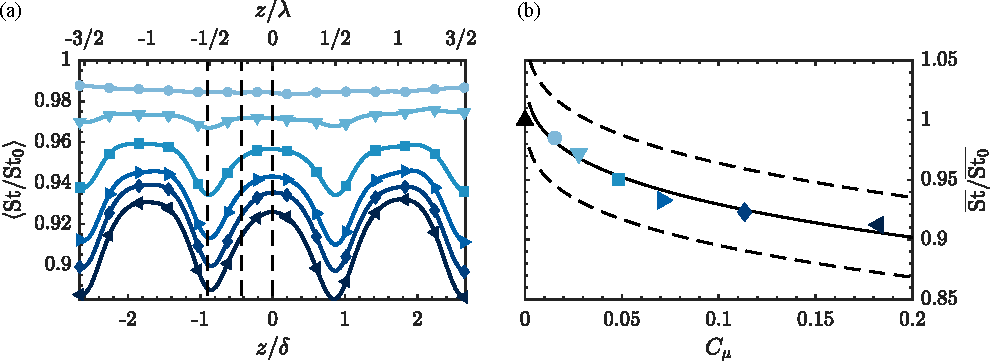
\includegraphics[width=0.99\linewidth]{figures/results/St/stz_v3_cmu.pdf}
         \caption{(a) Streamwise average of Stanton number in the region of interest shown in figure~\ref{fig:st_maps} normalised with the reference TBL; reference lines \lcap{--}{black} highlight $z_1$, $z_2$ and plane of symmetry spanwise stations from left to right. (b) Spatial average of the Stanton number in the region of interest as a function of the body force with the fit for the empirical relation $\overline{\mathrm{St}} \propto C_\mu ^{2/7} $ \lcap{-}{black} and $\pm3.7\%$ error interval \lcap{--}{black}. Symbols correspond to each discharge voltages $V_{pp}=$ (and momentum coefficient $C_\mu = $) 0 \sy{black}{t*}, 10 (0.0153) \sy{blue2}{o*}, 12 (0.0278) \sy{blue3}{dt*}, 14 (0.0484) \sy{blue4}{s*}, 16 (0.0711) \sy{blue5}{rt*}, 18 (0.1133)
         \sy{blue6}{d*}, 20 (0.1825) \sy{blue7}{lt*}.} \label{fig:meanSt_delta}
\end{figure}
%---

The uniform distribution of $\mathrm{St}$ measured for the weakest actuation suggests that the large-sale motion introduced at the control region is not sufficiently strong to persist downstream and rapidly diminishes. Nonetheless, the heat transfer reduction at the wall persists even after the dissipation of the plasma-induced flow, which was reported by \citet{Schoppa1998} for a spanwise control law in channel flows and recently concluded in \citet{cheng_wong_hussain_schroder_zhou_2021} for similar plasma-actuators vortex generators in TBLs. The large structures collapse just downstream of the DBD-actuator, diffusing into lower scales that uniformly distribute within the boundary layer, thus promoting a homogeneous reduction in heat transfer. As the forcing amplitude is increased, so is the intensity of the large-scale structures which are able to persist in space and time as can be assessed from their thermal footprint. The conclusions drawn from the IR thermography analysis confirm the proposed explanation exposed in \S\ref{s:TBLanalysis}, justifying the formation of pairs of counter-rotating vortices. 

Upon the activation of plasma discharge, a downwash occurs between electrodes (plasma side), as the plasma actuator entrains fluid from above, ejecting it laterally. It has been shown that the plasma causes a large streamwise velocity deficit in the buffer and logarithmic region of the boundary layer that is persistent downstream. This deficit is related to the formation of streamwise vortices, which also alters the near-wall velocity gradient, thus reducing turbulent fluxes as is the case of convective heat transfer at the wall. The plasma-induced vortices superpose their upwash/downwash from adjacent vortices, causing increased transport of high-momentum fluid towards the wall by vortex induction, and conversely, pushing more low-momentum fluid from the near-wall region away from the surface. This approach is very similar to that proposed by \citet{jukes2013plasmaVG}, in which the combination of two elongated electrodes in the direction of the flow leads to what they defined as \textit{DBD-plasma actuator vortex generator}, which was also exploited in turbulent boundary layers as for the case of \citet{Wicks2015}.
The mutual induction between vortex pairs at $z_1$ displaces the fluid from the lower region of the boundary layer to the outer region, extracting low-speed fluid with high turbulent intensity from the wall, locally minimising heat transfer. On the other hand, streamwise vortices are weaker at $z_2$. The plasma-induced suction enables the formation of the vortex, which locally enhances the mixing between the outer and lower regions of the TBL. 
 
The study by \citet{cheng_wong_hussain_schroder_zhou_2021} concludes that the local reduction in skin friction is due to the reorganisation of the TBL streaks within the turbulent boundary layer. The ‘artificial’ vortices introduced by the plasma actuation and their associated spanwise wall jets act as a mechanism of merging natural streaks. Furthermore, their flow visualisation results show that the resultant streak is wider and has reduced meandering in space. This wider streak resembles the low-speed ribbon centred at $z_1$ in the present study. \citet{cheng_wong_hussain_schroder_zhou_2021} attribute the effect of forcing as a stabilisation of the streak-alike structure, thus interrupting the turbulence regeneration cycle and reducing the production of turbulent fluxes. This conclusion is also supported by the TBL analysis performed in the present study. The streamwise velocity is locally reduced in the region where ejection occurs while it is increased at both sides due to the spanwise diversion of the flow. Such velocity and momentum flux deficit incurred by the plasma forcing are persistent in space and time as extracted from the values of $\delta^*$ and $\theta$ reported in table~\ref{tab:TBLparams}. Consequently, the local heat transfer at the wall is modified according to the local flow condition at the wall.

Figure~\ref{fig:meanSt_delta}(b) depicts the evolution of the spatially averaged Stanton number, defined as:
\begin{equation}
    	\overline{\mathrm{St}} = \iint {\mathrm{St}(x,z)} \,\mathrm{d}x\,\mathrm{d}z.
\end{equation}
Considering that the weakest actuation ($C_\mu = 0.015$, i.e. $V_{pp}=10\mathrm{kV}$) hereby reported is found to be the threshold value for generating a plasma discharge, the results show that the value of $\overline{\mathrm{St}}$ follows a linear relation with the discharge voltage. Recalling that the integrated body force in non-dimensional form, i.e. the momentum coefficient $C_\mu$, scales with the discharge voltage to the $7/2$ power as reported in figure~\ref{fig:plasma_char}, a proportional relation can be expressed between the spatially-averaged Stanton number and the momentum coefficient: $\overline{\mathrm{St}} \propto C_\mu^{2/7}$. This relation reasonably matches the experimental data as shown in figure~\ref{fig:meanSt_delta}(b), with the Stanton number being reduced with the momentum injection promoted by plasma. Eventually, the plasma forcing provides a reduction of 9\% in convective heat transfer for the strongest actuation, which reaches values of 11\% reduction along with the streaks (see figure \ref{fig:meanSt_delta}), in close agreement with the skin-friction drag reduction of 7\% reported in \citet{cheng_wong_hussain_schroder_zhou_2021}. 

The proposed actuation, characterised by a jet spacing of $\Delta z^+ \approx 450 ~(=\lambda^+/2)$ and an intensity of $8\%$ of the free stream velocity, resembles to the proof-of-principle test proposed by \citet{Schoppa1998} for drag reduction. They reported a significant sustained drag reduction of 20\% which they attested to the weakened longitudinal vortices near the wall due to forcing-induced suppression of an underlying streak instability mechanism. The production of wide ribbons of low-speed streamwise velocity take a relevant part in the drag reduction mechanism. This approach to reducing turbulent wall fluxes is common in studies that employ spanwise travelling waves \citep{Du2002, Whalley2014} or spanwise wall-jet forcing \citep{yao2017,yao2018}. These studies, although using a different control strategy, achieve similar results in terms of wall-fluxes reduction by the generation of mutually interacting streamwise vortices. Indeed, the alteration of the near-wall flow, transforming sublayer streaks into wide ribbons of low-speed fluid is a relevant and persistent conclusion in the present study.

%%%%%%%%%%%%%%%%%%%%%%%%%%%%%%%%%%%%%%%%%%%%%%%%%%%%%%%%%%%%%%%%%%%%%%%%%%%%%%
%%%%%%%%%%%%%%%%%%%%%%%%%%%%%%% CONCLUSIONS %%%%%%%%%%%%%%%%%%%%%%%%%%%%%%%%%%
%%%%%%%%%%%%%%%%%%%%%%%%%%%%%%%%%%%%%%%%%%%%%%%%%%%%%%%%%%%%%%%%%%%%%%%%%%%%%%%
\section{Conclusions} \label{s:conclusions}
The utilisation of plasma actuators as vortex generators to control convective heat transfer in a turbulent boundary layer is investigated experimentally. In particular, an array of plasma actuators is used to induce pairs of counter-rotating, stationary, streamwise vortices embedded in a turbulent boundary later. The analysis focuses on the mechanism of interaction between the plasma-induced large-scale structures and the convective heat transfer process in a fully developed turbulent boundary layer over a flat plate with ZPG conditions. The combination of flow-field and heat-transfer measurements allows to understand the physics behind the plasma-induced flow.

A convective heat transfer reduction mechanism is proposed. The current plasma control technique focuses on manipulating near-wall coherent structures, which are responsible for turbulent transport phenomena within the TBL. Large-scale pairs of counter-rotating streamwise vortices are generated upon the activation of the plasma discharge. The proposed DBD-plasma actuator array is shown to be robust, with long-life applicability without loss of effectiveness.

The generation of pairs of counter-rotating, streamwise vortices is confirmed by the reconstructed three-dimensional mean flow field. Upon the activation of plasma, the fluid ejected laterally by the discharge is replenished by entertainment from above the exposed electrodes. This generates a circulation in the lateral plane leading to a vortical motion. The coalescence of the plasma-induced circulation with the main stream leads to twisting and folding of the spanwise vorticity at the tip of each plasma actuator. Eventually, wall-normal mean vorticity is produced by the body force, which reorients into the streamwise direction, while the spanwise mean vorticity is also reoriented into the streamwise direction. These phenomena have been previously reported by \citet{jukes2013plasmaVG} for a single actuator aligned with the main flow and by \citet{Wicks2015} for an array similar to the one proposed here. Additionally, the induced streamwise vortices are confirmed to be stationary according to the persistence theory of turbulence \citep{Cotel1996stationary}. The suction promoted over the exposed electrodes of the plasma-actuator array locally confines the vortices, preventing them to expand in the spanwise direction. The stationary vortices reduce wall fluxes as demonstrated for the convective heat transfer wall distribution downstream. 

Furthermore, an in-depth analysis of the turbulent boundary layer and its statistical parameters is performed. The plasma-induced flow diverts the TBL within the inner region, close to the wall and two main effects are outlined: on one hand, at the location where the wall-tangent opposing plasma-induced jets collide (namely, $z_1$), a mass and momentum flux deficit is observed due to a considerable reduction of the streamwise velocity component by the upwelling motion induced by the plasma; and, on the other hand, over the exposed electrodes (namely, $z_2$), a moderate reduction of mass and momentum flux deficit is detected as a consequence of the flow diversion and subsequent acceleration. The former effect causes a considerable increase of $\delta^*$ and $\theta$ with respect to the non-actuated TBL while the latter yields the opposite result.

These conclusions are in agreement with the recent contribution by \citet{cheng_wong_hussain_schroder_zhou_2021}, albeit conducted here at significantly larger freestream velocity and momentum injection. The wall-tangent injection of momentum by plasma forces the TBL streaks together, which eventually merge and stabilise. A wide ribbon of low-speed fluid is promoted and stabilised by plasma actuation at $z_1$. The generation of wide ribbons of low-speed fluid is a common strategy as a drag reduction mechanism \cite[e.g.][]{Schoppa1998,Du2002, Whalley2014,cheng_wong_hussain_schroder_zhou_2021} and, analogously, it is concluded that it is a strategy that is also efficient for reducing heat fluxes at the wall.

Considering the IR thermography analysis, it is concluded that the plasma-induced flow is persistent downstream, with remarkable consequences on the heat transfer distribution. Wide ribbons of Stanton number reductions are observed at $z_1$, suggesting that the velocity deficit promoted by plasma endures downstream of the actuation with an effective reduction of wall fluxes. Despite the spanwise modulated Stanton number distribution, a consistent reduction of spatially integrated heat transfer is observed for increasing intensity of the forcing amplitude. Eventually, it is concluded that the Stanton number over an actuator pitch scales linearly with the discharge voltage, i.e. with the $2/7$ power of the momentum coefficient $C_\mu$. This interesting result summarises with an overall reduction of $\approx10\%$ of the Stanton number far downstream of the actuation and for a wide region of interest. 

%%%%%%%%%%%%%%%%%%%%%%%%%%%%%%%%%%%%%%%%%%%%%%%%%%%%%%%%%%%%%%%%%%%%%%%%%%%%%%%
%%%%%%%%%%%%%%%%%%%%%%%%%% Acknowledgements %%%%%%%%%%%%%%%%%%%%%%%%%%%%%%%%%%%
%%%%%%%%%%%%%%%%%%%%%%%%%%%%%%%%%%%%%%%%%%%%%%%%%%%%%%%%%%%%%%%%%%%%%%%%%%%%%%%

\section*{Acknowledgements}
Rodrigo Castellanos, Stefano Discetti and Andrea Ianiro have been supported by the project ARTURO, ref. PID2019-109717RB-I00/AEI/10.13039/501100011033, funded by the Spanish State Research Agency.
Theodoros Michelis and Marios Kotsonis are supported by the European Research Council under StG project GloWing (\#803082).

\section*{Declaration of Interest}
The authors report no conflict of interest.


%------------------------------------------------------------------------------
% Bibliography
%------------------------------------------------------------------------------
%
%\clearpage
\bibliographystyle{jfm}
\bibliography{paper2/bib2}
%
\IfFileExists{paper2/bib2.bbl}{\input{paper2/bib2.bbl}}{}


%===============================================================================
%                            END PAPER
%===============================================================================
\end{paper}

%-------------------------------------------------------------------------------
% Paper 3: CF jets
%------------------------------------------------------------------------------
% Define title, author(s), affiliation and publishing status
%
\papertitle[On the uncertainty of BL parameters from EPTV data] % Short title used in headlines (optional)
{%
  On the uncertainty of boundary-layer parameters from Ensemble PTV data % THE COMMENT SYMBOL AT THE END OF THIS LINE IS NEEDED
}%
%
\papertoctitle{On the uncertainty of boundary-layer parameters from Ensemble PTV data} % Title for toc
%
\paperauthor[R. Castellanos \etal] % Short authors used in headlines and List Of Papers
{%
  R. Castellanos$^1$, C. Sanmiguel Vila$^1$, A. G\"uemes$^1$ \& S. Discetti$^1$%
}%
%
\listpaperauthor{Castellanos, R., Sanmiguel Vila, C., G\"uemes, A. \& Discetti, S.}% (optional) Short authors used in List Of Papers
%
\paperaffiliation
{%
  $^1$ Aerospace Engineering Research Group, Universidad Carlos III de Madrid (UC3M), Avda. Universidad, 30, 28911 Leganes, Madrid, Spain\\
}%
%
\paperjournal[Meas. Sci. Technol.] % Short publish info used in List Of Papers
{%
	Measurements Science and Technology%
}%
%
\papervolume{32}%
%
\papernumber{8}%
%
\paperpages{084006}%
%
\paperyear{2021}%
%
% \paperdoi{10.1088/1361-6501/abfad0}
%
\papersummary%
{% Insert summary of the paper here (used in introduction)
    The recent advancements in high-resolution turbulent-statistics computation from ensemble particle tracking velocimetry (EPTV) data are now opening new possibilities in turbulent-flow characterisation. Measurements of full-field boundary layer profiles with a fine resolution close to the wall and up to the freestream with one single imaging setup are now feasible, thus paving {the way} to direct characterisation of turbulent-boundary-layer (TBL) parameters with composite-profile formulations. In this work, we build a framework for the estimation of the uncertainty of EPTV in performing this task. The effect of systematic errors due to finite spatial resolution and of random error due to convergence are investigated under different window size. {Then we introduce random errors to simulate the effects on convergence issues on the velocity profile and, consequently, on the estimation of turbulent-boundary-layer parameters. The statistical dispersion of the estimated parameters provides an estimation of the uncertainty range.} We validate with experimental data {this} flexible tool to estimate \textit{a priori} the expected uncertainty level of the most relevant {turbulent-boundary-layer} parameters in zero-pressure-gradient TBL, being the method based on existing profiles from high-fidelity simulation or from analytical {composite-profile} formulations when such data are not available.
}%
%
\graphicspath{{paper1/}}%
%
%
%===============================================================================
%                            BEGIN PAPER
%===============================================================================
%
\begin{paper}

\makepapertitle

%------------------------------------------------------------------------------
% Abstract
%------------------------------------------------------------------------------
%
\begin{paperabstract}
    The recent advancements in high-resolution turbulent-statistics computation from ensemble particle tracking velocimetry (EPTV) data are now opening new possibilities in turbulent-flow characterisation. Measurements of full-field boundary layer profiles with a fine resolution close to the wall and up to the freestream with one single imaging setup are now feasible, thus paving {the way} to direct characterisation of turbulent-boundary-layer (TBL) parameters with composite-profile formulations. In this work, we build a framework for the estimation of the uncertainty of EPTV in performing this task. The effect of systematic errors due to finite spatial resolution and of random error due to convergence are investigated under different window size. {Then we introduce random errors to simulate the effects on convergence issues on the velocity profile and, consequently, on the estimation of turbulent-boundary-layer parameters. The statistical dispersion of the estimated parameters provides an estimation of the uncertainty range.} We validate with experimental data {this} flexible tool to estimate \textit{a priori} the expected uncertainty level of the most relevant {turbulent-boundary-layer} parameters in zero-pressure-gradient TBL, being the method based on existing profiles from high-fidelity simulation or from analytical {composite-profile} formulations when such data are not available.
    \keywords{ensemble particle tracking velocimetry, PIV, turbulent boundary layer, wall-bounded flows}
\end{paperabstract}


%------------------------------------------------------------------------------
% Article
%------------------------------------------------------------------------------
%
\definecolor{blue}{rgb}{0,0,1}
\definecolor{red}{rgb}{1,0,0}
\definecolor{black}{rgb}{0,0,0}
\definecolor{grey}{rgb}{0.5,0.5,0.5}
\definecolor{dark}{rgb}{0.25,0,0.37}
\definecolor{orange}{rgb}{0.58,0.08,0.3}
\definecolor{yellow}{rgb}{1,0.59,0}
\definecolor{purple}{rgb}{0.92,.24,0.18}
\definecolor{blue1}{rgb}{0.81,0.9,0.95}
\definecolor{blue2}{rgb}{0.65,0.81,0.91}
\definecolor{blue3}{rgb}{0.38,0.69,0.83}
\definecolor{blue4}{rgb}{0.13,0.56,0.76}
\definecolor{blue5}{rgb}{0,.39,0.67}
\definecolor{blue6}{rgb}{0,.25,0.5}
\section{Introduction}
Accurately determining the parameters that describe an experimental turbulent boundary layer (TBL) is crucial to modelling and understanding these flows \citep{titchener2015calculation,pan2020unscented}. In particular, the parameters that can be employed to characterise the mean velocity profile of a TBL can be used, among other purposes, to determine whether a TBL can be considered as well-behaved, (i.e. not in a post-transitional state or affected by non-equilibrium effects) \citep{Chauhan:2009p10824,Sanmiguel:2017JFM}, to compare the results between different experimental or numerical datasets \citep{Schlatter:2009p13969} or to calculate dimensionless numbers that are used to analyse the effect of disturbances such as the inclusion of obstacles or pressure gradients \citep{Clauser:1954p10911,guemes2019flow}. These parameters include quantities such as: the friction velocity $u_\tau$, defined as $u_\tau = \sqrt{\tau_w/\rho}$ (being $\tau_w$ the mean wall-shear stress and $\rho$ the fluid density); the boundary layer thickness $\delta$, which is the wall-normal distance beyond which viscous effects can be considered as negligible; and the freestream velocity $U_\infty$. Among the classical TBL parameters it is also common to define the so-called integral lengths, such as the displacement thickness $\delta^*$ and the momentum thickness $\theta$, providing information regarding the mass and momentum transfer within the boundary layer. The integral lengths are defined for an incompressible flow as,
\begin{equation}
    \delta^* = \int_{0}^{\infty} \left(1-\frac{U}{U_\infty}\right) \,dy;
\end{equation}
\begin{equation}
 \theta = \int_{0}^{\infty} \frac{U}{U_\infty}\left(1-\frac{U}{U_\infty}\right) \,dy.
\end{equation}

being $U = U(y)$ the velocity distribution as a function of the wall-normal coordinate $y$. Since in turbulent boundary layers, $U$ does not {necessarily reach an asymptotic value} at the boundary-layer edge, the previous formulation can be truncated at the boundary layer thickness $\delta$ for its upper integration limit such that,
\begin{equation}
\label{integral}
    \delta^* = \int_{0}^{\delta} \left(1-\frac{U}{U_e}\right) \,dy;~~ \theta = \int_{0}^{\delta} \frac{U}{U_e}\left(1-\frac{U}{U_e}\right) \,dy
\end{equation}
and in consequence the boundary-layer edge velocity is defined as $U_e = U(y=\delta)$.

Using the previously defined TBL parameters, it is possible to generate new figures of merit, such as the shape factor defined as $H_{12}=\delta^*/\theta$ or the skin-friction coefficient $C_f = \tau_w/(\frac{1}{2} \rho U_\infty^2)$, that allow the assessment of the flow regime or discern whether a particular TBL can be considered to be canonical \citep{Chauhan:2009p10824}. Such quantities are used due to their high sensitivity to different boundary and inflow conditions \citep{Chauhan:2009p10824}.

Regardless of the measurement technique, these boundary-layer parameters are  strongly affected by errors due to discretization of the velocity profile, the spacing between the points, the distance of the first point from the wall, and uncertainty in the wall location \citep{titchener2015calculation,Orlu:2010p36071}. In addition to these sources of error, there is no consensus when it comes to the methodology for calculating $\delta$. Several of the proposed methods rely on the use of additional quantities besides the mean velocity profile, such as the mean vorticity \citep{spalart1993experimental}, the mean streamwise variance \citep{Vinuesa:2016is} or a reference pressure \citep{griffin2020general}. On the other hand, accurate determination of friction-related quantities (such as $u_\tau$ and $\tau_w$) is also particularly challenging \citep{orlu2020instantaneous}. Different experimental approaches that can be employed to measure these quantities, such as oil-film interferometry \citep{Vinuesa:2016tn}, Preston tube \citep{head1962preston},  MEMS shear-stress sensor \citep{sheplak2004mems}.

For {the particular case of zero-pressure gradient (ZPG) TBLs and in} those situations where only mean streamwise velocity measurements are available, an alternative to calculate all the boundary-layer parameters is to resort to composite velocity profiles based on analytical expressions \citep{Chauhan:2009p10824,Coles:2006p898,Nickels:2004p15662,Rodriguez-Lopez2015}. This methodology is based on assuming that the mean streamwise velocity profile can be described using a function that takes the form of $U^+(y^+)= U^+_{inner}+U^+_{outer}$, which is used to fit the data of the aforementioned profile. In the present study the superscript $+$ denotes inner scaling, which is defined as $U^+=U/u_\tau$ and $y/\ell^*$, being $\ell^*$ the viscous length $\ell^* = \nu/u_\tau$ and $\nu$ the kinematic viscosity. The term $U^+_{inner}$ is the part of the function that provides a description of the velocity profile from the viscous sublayer up to the overlap region, while the term $U^+_{outer}$ is used to define the outer region of the TBL profile. The $U^+_{inner}$ function is typically based on $U^+=y^+$ for the inner region and on the logarithmic law $U^+=\frac{1}{\kappa}y^+ +B$ for the overlap region, where $\kappa$ is the von Kármán constant and $B$ is an integration constant. The $U^+_{outer}$ function was introduced by \citet{Coles:2006p898} with the inclusion of the wake function $\mathcal{W}$, defining the wake component of the velocity profile. There are different formulations of the wake function since the wake component is greatly affected by boundary or initial conditions. Depending on the study, the complexity of the $U^+$ formulation can be varied and even some of the parameters can be previously defined from established correlations to reduce the dimensionality of the fitting process. The major advantage of this methodology is that, by using just a full-resolution mean velocity profile, it is possible to estimate the {boundary-layer} parameters and to correct the wall location. 

Hardware and software advances have recently opened the path to full-resolution {TBL velocity-profile} measurements at sufficiently large friction Reynolds number using Particle Image Velocimetry (PIV). In particular, techniques based on ensemble averaging (e.g. single-pixel correlation \citep{westerweel2004single}, or ensemble particle tracking velocimetry, EPTV \citep{cowen1997hybrid,kahler2012uncertainty}) are able to achieve a sufficiently large dynamic range to resolve the entire velocity profile, from the viscous sublayer up to the freestream, thus enabling {composite-profile} application. Single-pixel correlation is based on ensemble averaging of cross-correlation maps. EPTV is based on identifying vectors from instantaneous realisation and superposing them to build a dense cloud of vectors. Statistical information is then inferred from the pdf of the velocity vectors in averaging windows, referred as \textit{bins} (either isotropic, anisotropic or with shape adapted locally \citep{raiola2020adaptive}). 
Reynolds stresses can also be measured accurately if velocity gradient effects within the averaging bin are taken into account. In single-pixel correlation, this can be achieved by proper modelling of the shape of the cross-correlation peak \citep{scharnowski2012reynolds}, while in EPTV the velocity-gradient effect can be reduced by local polynomial fitting of the vectors to be averaged \citep{aguera2016ensemble}. It was recently shown in mild {adverse-pressure-gradient TBLs} \citep{SanmiguelVila2017} that this second approach is generally more robust; furthermore, the recent advances in volumetric velocimetry \citep{discetti2018volumetric} are now pushing towards a widespread use of Lagrangian Particle Tracking (LPT), thus motivating an increased interest in understanding the capabilities of EPTV approaches in measuring velocity profiles. PIV/PTV offer the indisputable advantage of providing also information on the instantaneous flow field organisation; this renders worth exploring the uncertainty of PIV/PTV/LPT in determining parameters which are normally measured using the portfolio of techniques mentioned above.

In this work, the uncertainty in extracting boundary-layer parameters from ``full-field'' EPTV data is explored, i.e. assuming that the field of view covers the entire {boundary-layer} thickness plus a robust freestream measurement. {For the sake of simplicity, the present study is focused on well-behaved ZPG TBLs in which a composite-profile approach can be applied, as in hot-wire measurements.} While it is common to use separate experiments for high-resolution near-wall measurements (see for instance the work by \citet{kahler2006wall}) and for the {full-field} organisation, the approach we present here has the advantage of requiring the same image dataset for statistics extraction and flow field characterisation.
We will first simulate in virtual experiments the effect of finite spatial resolution on data generated from Direct Numerical Simulations (DNS) of a {ZPG TBL} and using a composite profile {formulation of a ZPG TBL}. Systematic errors due to the bin-averaging effect and the position of the first measurement point with respect to the wall are addressed in \S \ref{s:SyntheticValidation} as a function of the bin size. {In this section random errors due to finite convergence or wall-positioning uncertainty are not introduced, as the focus is simply on systematic error.}

Then {in \S \ref{s:validation}} a {Monte Carlo} study is conducted to estimate the uncertainty of the composite profile fitting due to finite number of samples. This is particularly relevant in EPTV, since the bin size depends on the number of snapshots and the number of vectors within the bin, considered sufficient for a satisfactory accuracy. {The method will thus deliver an uncertainty range for each turbulent-boundary-layer parameter. An experimental validation is carried out to verify that the error on the ZPG TBL parameters are predicted within an uncertainty range for a wide range of bin sizes.} 

%--------------------------------------------------------------------------------
%------------------------------- METHODOLOGY ------------------------------------
%--------------------------------------------------------------------------------
\section{Methodology}
The methodology to estimate the uncertainty of EPTV measurements for TBL characterisation is illustrated in this section. The method is based on simulating the errors due to finite resolution and convergence on existing TBL profiles, either based on DNS {ZPG} data or on analytical formulation of {ZPG TBL} composite profiles. Different levels of camera resolutions and bin sizes are explored in order to investigate systematic errors in the fitting procedure and the random uncertainty due to convergence issues. {In the proposed method no particle images are generated; the effects of the error sources are directly simulated by averaging existing velocity profiles (or generated ad hoc with composite profile formulations). This renders the method of simple and general application, avoiding the need of generating virtual images for the specific case.}

\subsection{Synthetic profile generation} \label{ss:synthetic_method}

The synthetic TBL profile is generated from existing datasets to replicate the incurred errors from experiments using EPTV. The synthetic profile is generated using as a reference:

\begin{itemize}
    \item Dataset of {ZPG TBL} DNS simulations, available in the turbulent database of the Fluid Dynamics Group from Universidad Politécnica de Madrid\footnote{\url{https://torroja.dmt.upm.es/turbdata/blayers/}}. In particular, for the analysis conducted in the following, the data corresponding to $Re_{\vartheta}=4500$ have been used \citep{sillero2013one}.
    \item Composite-profile generated data based on the ZPG TBL formulation by \citet{Chauhan:2009p10824} which will be briefly outlined in \S \ref{s:composite_profile}.
\end{itemize}

{The velocity vectors are directly generated from the interpolation of the DNS data in the first case, and from the analytical formulation of the composite profile in the second case.} In all cases, the simulated field of view spans from the wall to $1.3\delta$. This upper bound is set in order to guarantee a sufficiently robust measurement of the freestream. The resolution is here defined in wall units as {$Res = \frac{S}{1.3 Re_\tau}$}, being $S$ the available pixels in the camera sensor in the wall-normal direction. 

The systematic error due to bin averaging in the binning process of the EPTV is simulated by top-hat averaging of the velocity profiles within bins of different size. We tested bin sizes ranging between {$1\ell^*$ to $200\ell^*$}. The bin size distribution in wall units is reported in Figure \ref{fig:window} as a function of the size in pixels and of the spatial resolution expressed in pixels per wall unit.

The profiles are truncated removing from the near-wall region bins which were not completely included in the domain. While this would imply removing vectors with distance from the wall smaller than one half of the window size, after the analysis of the experimental results, we decided to introduce a more restrictive criterion and cut the profiles to a distance of 3/4 of the window size. This criterion excludes from the analysis pixels in close proximity from the wall, which are very likely to be affected by spurious reflection effects in PIV measurements. Due to the sensitivity of the composite-profile formulation to the quality of the near-wall data, this criterion was found to be more robust. 

The effect on the streamwise mean velocity profile of the bin averaging is shown in Figure~\ref{fig:F1_DNSprofiles} for DNS data. The effect of increasing the bin size is clear in the near-wall region, where the measured profile departs from the baseline due to averaging effects. It is expected that this systematic error, combined with the lack of points in the near-wall region for relatively large bin size, will yield more significant errors in determining the friction velocity and the wall position. Also, the computation of integral quantities is sensitive to the position of the nearest point to the wall \citep{titchener2015calculation,Rodriguez-Lopez2015}. 

\begin{figure}
    \centering
    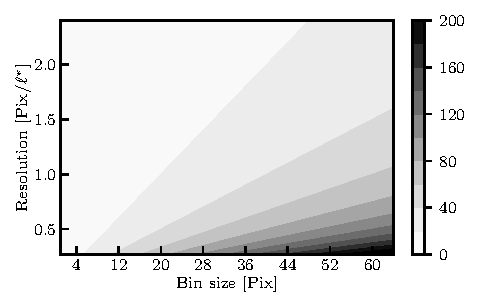
\includegraphics[width=0.75\columnwidth]{Figures/figure08.pdf}
    \caption{Bin size distribution {expressed in wall units $l^*$} with respect to bin size in pixels and resolution.}
    \label{fig:window}
\end{figure}


\begin{figure}
    \centering
    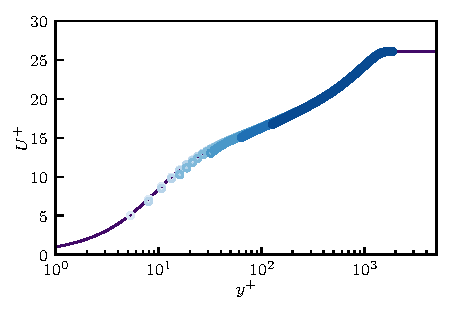
\includegraphics[width=0.75\columnwidth]{Figures/figure05.pdf}
    \caption{Effect on the streamwise mean velocity profile of the bin averaging in EPTV with 2 \sy{blue1}{o}, 4 \sy{blue2}{o}, 8 \sy{blue3}{o}, 16 \sy{blue4}{o}, {32} \sy{blue5}{o}, and 64 \sy{blue6}{o} pixels bin size for a fixed value of $S=700$. Ground truth DNS data is referred as \lcap{-}{dark}.}
    \label{fig:F1_DNSprofiles}
\end{figure}

Two contributions of random error have been included. The first error is a perturbation of the initial guess of the wall position, which is most often inferred from visual inspection of the images. This process might be severely affected by the image quality near the wall; furthermore, depending on the surface material and quality, the wall position might not be completely clear. {Throughout this work} we introduced a uniformly distributed random error with bounds $\pm0.5$ pixels, even though the presented uncertainty estimation method can be tuned to model more optimistic/pessimistic scenarios. The second contribution of random error is due to convergence, which depends on the random error on the velocity vectors (assumed here having Gaussian distribution with standard deviation $\sigma_v$) and on the turbulent fluctuation levels. If we indicated with $u'$ the standard deviation of the streamwise turbulent fluctuations, the expected standard deviation of the error of the mean is:
\begin{equation}
\label{ruido}
    \sigma_{U}=\frac{\sqrt{u'^2+\sigma_v^2}}{\sqrt{N_v}}    
\end{equation}
with $N_v$ being the number of vectors in each bin (supposing for simplicity it is sufficiently small to ensure that on average it contains less than 1 vector per snapshot). 
For the DNS data, the profile of $u'$ is available and can be directly plugged in Eq.~\ref{ruido}; however, for the case simulated with the composite profile proposed by \citet{Chauhan:2009p10824}, since an analytical formulation for second-order statistics is not readily available, the standard deviation of the error of the mean is modelled assuming a two-level distribution with piecewise constant $u'$. A level of $u'^+=2$ for $y<0.9 \delta$ is chosen as an average value of the streamwise turbulent fluctuations for the $Re_\tau$ under study and a value of $u'^+=0.5$ as a representative value of the freestream velocity is used for the locations $y\geq 0.9 \delta$.

A {Monte Carlo} approach is followed to characterise the uncertainty on the estimation of the {ZPG }TBL parameters. The systematic and random uncertainty are defined respectively using the median and the standard deviation of the results of the simulated experiments. {The systematic errors are addressed in \S \ref{s:SyntheticValidation}, while the effect on random uncertainty is introduced in \S \ref{s:validation}.}

\subsection{Calculation of the boundary-layer parameters}
\label{s:composite_profile}

In order to calculate the different boundary-layer parameters and to correct the wall location using only the mean streamwise velocity profile, a two-step strategy based on the use of two different composite profiles is followed. In a first step, the mean velocity data after the EPTV process is fitted to the composite profile proposed by \citet{Chauhan:2009p10824} {for ZPG TBLs }and defined as follows,

\begin{equation} \label{eq:chauhan}
U^+=U^+_{inner}+\frac{2\Pi}{\kappa} \mathcal{W} \left( \eta \right), 
\end{equation}
being $\Pi$ the wake parameter and $\eta=y^+/\delta^+$. Using this formulations the $U^+_{inner}$ and $\mathcal{W}\left(\eta \right)$ read as follows,

\begin{equation}
\label{innerchuahan}
\begin{array}{ll}
U^+_{inner}=& \frac{1}{\kappa} \ln\left(\frac{y^+-a}{-a}\right)  + \frac{R^2}{a(4\alpha+a)} 
 (4\alpha+a)  \\
& \left[ \ln \left(-\frac{a}{R}\frac{\sqrt{(y^+ -\alpha)^2+\beta^2}}{y^+-a}\right) +\frac{\alpha}{\beta}(4\alpha+5a) \right. \\
& \left. \left(\arctan\left(\frac{y^+-\alpha}{\beta}\right)+\arctan\left(\frac{\alpha}{\beta}\right)\right) \right]+ \\ &\frac{\exp[-\ln^2(y^+/30)]}{2.85},
\end{array}
\end{equation} 
where $\alpha=(-1/\kappa-a)/2$, $\beta=\sqrt{-2a\alpha-\alpha^2}$, $R=\sqrt{\alpha^2+\beta^2}$, $\kappa=0.384$ and $a=-10.3061$. The wake function $\mathcal{W}$ is defined as,

\begin{equation}
\label{outerchauhan}
\begin{array}{ll}
\mathcal{W}(\eta)= & \frac{1-\exp\left[-(1/4)(5a_2+6a_3+7a_4)\eta^4+a_2\eta^5 +a_3\eta^6+a_4\eta^7
	\right]}{1-\exp[-(a_2+2a_3+3a_4)/4]}  \\
& \times \left(1-\frac{1}{2\Pi}\ln(\eta)\right) 
\end{array}
\end{equation} 
where $a_2=132.8410$, $a_3=-166.2041$ and $a_4=71.9114$. The values of the constants have been derived by \citet{Chauhan:2009p10824} from several experiments over a large Reynolds number range and their formulation has been tested and proved to be robust when it comes to identify well-behaved profiles  \citep{Chauhan:2009p10824}. This composite-profile formulation is used to determine the values of $u_\tau$ and to correct the absolute wall position correction $\Delta y $ by means of a least-square procedure \citep{Chauhan:2009p10824,Orlu:2010p36071,Rodriguez-Lopez2015}. Since the values of the constants are fixed, this formulation allows to calculate $u_\tau$ without relying on locating the overlap region.

In the second step, the extracted values of $u_\tau$ and $\Delta y$ are used to calculate the corresponding $U^+$ and $y^+$ and then fit them to the composite profile proposed by \citet{Nickels:2004p15662}, which has the following formulation for the particular case of a {ZPG TBL}, 

\begin{equation}
\label{Nickels}
\begin{array}{lll}
U^+ = & y^+_c \left[1- (1+2(y^+/y_c^+)+\frac{3}{2}(y^+/y^+_c)^2)e^{-3y^+/y_c^+}  \right] \\
& \times \frac{1}{6\kappa
_0} \left(\ln(\frac{1+(0.6(y^+/y_c^+))^6}{1+\eta^6})+b(1-e^{-\frac{5(\eta^4+\eta^8)}{1+5\eta^3}})\right) 
\end{array}
\end{equation} 
in which $b$ is a measure of the wake strength and is equivalent to wake parameter, $\kappa_0=0.39$ and $y_c^+=12$. 
This composite profile is used for the calculation of the edge velocity $U_e$ and the boundary-layer thickness $\delta$ because of its description of the wake region. The wake function proposed by \citet{Nickels:2004p15662} has been proved to be robust at low Reynolds numbers for both experimental and numerical profiles \citep{Schlatter:2010p35519}. Eventually, the resulting fitted velocity profile is integrated according to Eq.~\ref{integral} and using the $\delta$ and $U_e$ for the integration limits to extract $\delta^*$ and $\theta$. 

\section{Systematic error estimation for synthetic data}
\label{s:SyntheticValidation}

\begin{figure}
    \centering
    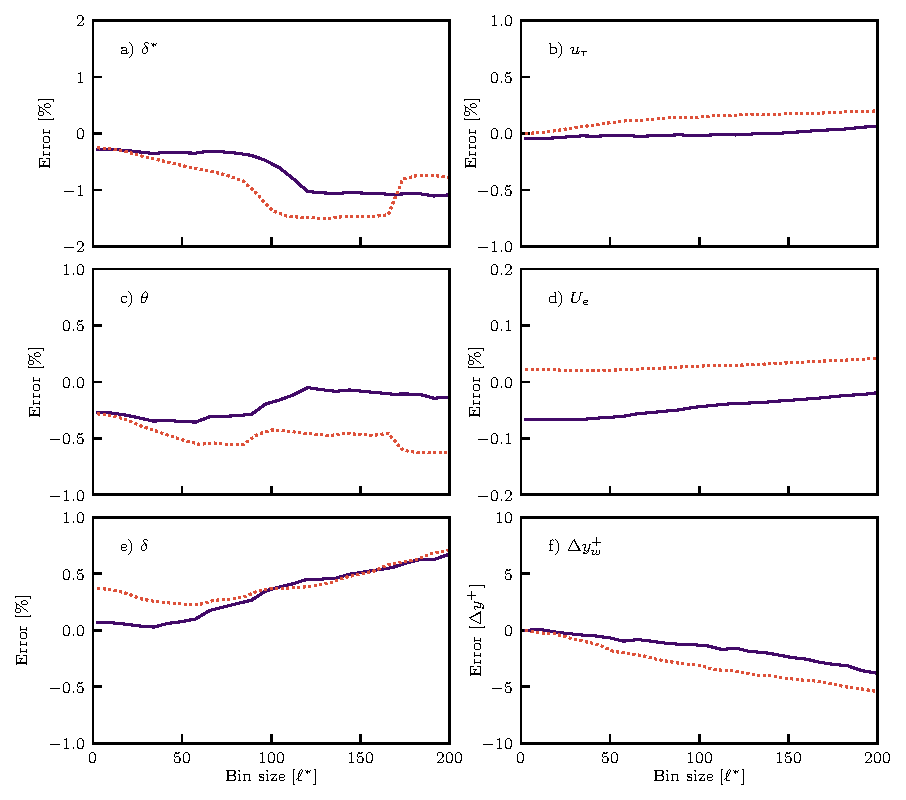
\includegraphics[width=\textwidth]{Figures/figure09.pdf}
    \caption{Systematic error as a function of the bin size for a) displacement thickness, b) friction velocity, c) momentum thickness, d) freestream velocity, e) boundary layer thickness, and f) y origin. Symbols refer to DNS \lcap{-}{dark}, Composite-profile \lcap{:}{purple}.}
    \label{fig:systematic_error}
\end{figure}

The procedure described in \S\ref{ss:synthetic_method} is explored {for different bin size in wall units}. {The objective of this section is to explore the systematic error due to the filtering effect on the profile due to finite bin size.} For this reason, the error sources due to convergence and to the wall-normal coordinate are not considered. Therefore, {the computation of TBL parameters} is performed {averaging on} a reduced set of {50} cases with a small random perturbation on the velocity profile ($N_v \sim O(10^6)$) to avoid bias errors due to locking in local minima in the fitting optimization procedure described in \S\ref{s:composite_profile}.

As reported in Figure~\ref{fig:F1_DNSprofiles}, the size increase of the averaging bin promotes two main effects on the velocity profile: the suppression of valid points in the near-wall region based on the criterion describes in \S\ref{ss:synthetic_method}; and the diversion of the near-wall points of the profile. 
As the {bin} size increases, at certain point, the averaging process in the logarithmic region will be affected by points within the buffer region, which eventually tend to curve the profile. As a consequence, the slope of the velocity profile in the logarithmic region will not follow the logarithmic law. This strongly affects the fitting procedure proposed by \citet{Chauhan:2009p10824}, especially for a proper estimation of the wall location and the friction velocity, since it assumes a velocity profile which fulfils the logarithmic law of the wall.

An overview of the performed parametric study is reported in Figure~\ref{fig:systematic_error}, based on data generated according to DNS of a TBL and the composite profile described in \S\ref{s:composite_profile}, respectively. The relative error is computed with respect to the reference parameters reported in Table~\ref{tab:1}.

The systematic error {profiles as a function of the bin size in wall units} are overall consistent between DNS and composite-profile data. This is particularly interesting since the composite profile can be easily generated for conditions matching the experiments, while high-fidelity simulations data might not be available, especially at high Reynolds numbers.

For the parameters computed from the first fit based on \citet{Chauhan:2009p10824}, i.e. $u_\tau$ and $\Delta y^+$, we observe a clear tendency of increasing magnitude of the error as the averaging bin increases in size. Nonetheless, the systematic error in $u_\tau$ estimation does not exceed 1\% and the correction of wall-normal coordinate is below $5^+$ for bin size smaller than {100}$\ell^*$. This result {suggests} that, although the bin size will affect the performance in the estimation of the parameters, the composite profile proposed by \citet{Chauhan:2009p10824} is robust in the inner region of the velocity profile. Only when the bin size affects the logarithmic layer, the fit is not capable of correcting for the wall position with an acceptable level of accuracy. {It is important to remark here that the estimation of $u_\tau$ with the composite profile is robust since the data correspond to ZPG conditions. In presence of pressure-gradient, curvature, roughness or other effects it is well known that the composite profile is less robust and the availability of points in the near-wall region becomes of paramount importance.} 

For the TBL parameters estimated in the second step by using the fit proposed by \citet{Nickels:2004p15662}, we find $\delta^*$ and $\theta$, with a relatively low error for {bin} sizes that lie below the logarithmic region; however, as the bin size exceeds 50$\ell^*$, the error becomes more significant. This is a direct consequence of the curvature smoothing effect promoted by the top-hat averaging as shown in Figure~\ref{fig:F1_DNSprofiles}, which is reducing the effectiveness of the second {inner} fit. Additionally, we find a systematic overestimation of both $\delta$ and $U_e$ {for the composite-profile case (although for the case based on the DNS profile $U_e$ appears to be slightly underestimated)}. This might be surprising at a first glance, since averaging effects are much less relevant at the edge of the boundary layer. This suggests that the truncation and bias errors in the near-wall region of the TBL are also affecting the results of the composite-profile fitting in the outer region. 

\begin{table}
\centering
% table caption is above the table
\caption{\centering Reference TBL parameters for DNS, composite profile and experiments.}
\label{tab:1}       % Give a unique label
% For LaTeX tables use
\resizebox{\textwidth}{!}{%
\begin{tabular}{lcccccccccc}
\hline\noalign{\smallskip}
 Case & $Re_{\tau}$ & $Re_{\theta}$ & $H_{12}$ & $\delta^*/\delta$ & $\theta/\delta$ & $u_{\tau}$[m/s] & $U_{e}$ [m/s] & $\delta$ [mm]  & $\ell^*$ [$\mu$m] & $C_f \cdot 10^3$\\
\noalign{\smallskip}\hline\noalign{\smallskip}
DNS          & 1437 & 4500 & 1.381 & 0.169 & 0.122 & - & -& - & - & 2.98 \\
{Composite-profile}        & 1445 & 4503 & 1.375 & 0.165 & 0.120 & 0.70  & 18.14 & 32 & 22 & 2.98\\ 
Experiments          & 1379 & 4432 & 1.390 & 0.170 & 0.123 & 0.042 & 1.11 & 29 & 21 & 2.91\\
\noalign{\smallskip}\hline
\end{tabular}}
\end{table}

\section{{Random uncertainty measurements - }experimental Validation} \label{s:validation}

{In this section the capabilities of the proposed methods to estimate the uncertainty range of each TBL parameter are tested. For this purpose, differently to the previous section, random errors on the velocity profiles due to finite convergence and wall-positioning are included, with a number of vectors per bin matching experimental conditions. A large number of tests is carried out to obtain statistics of the errors on the TBL parameters, thus delivering uncertainty ranges for each of them. An experimental validation is carried out using a high-resolution ZPG-TBL measurement as ground truth, and investigating the error introduced when increasing the bin size.}

\subsection{Experimental setup}

\begin{figure}
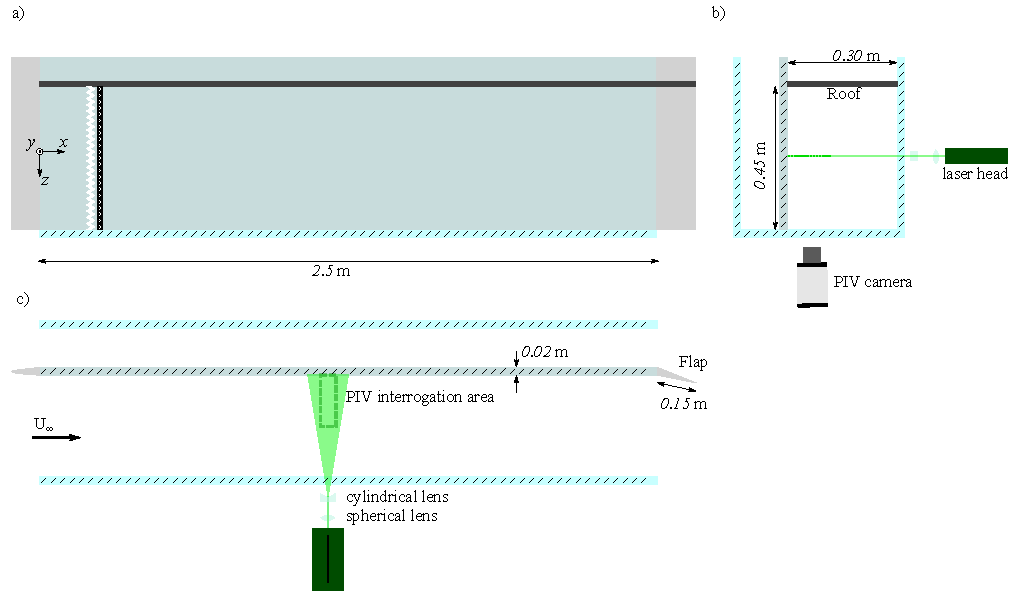
\includegraphics[width = 0.99\linewidth]{Figures/setup.pdf}
\caption{Sketch of the experimental setup. The flat plate is indicated in cyan, the walls of the water tunnel in light blue, and the 3D printed leading edge and flap in grey. a) Frontal view with reference system. The zig-zag tripping and dymo strips are included for reference. b) Lateral view, with illumination and imaging system. c) Top view, with optical arrangement and PIV measurement area.
}\label{fig:expsetup}
\end{figure}



An experimental campaign is held in the water tunnel at Universidad Carlos III de Madrid. The facility has a rectangular test section ($500 \times 550$~mm$^2$) with a length of $2.5$~m. A sketch of the experimental setup is reported in Figure~\ref{fig:expsetup}.  A flat plate is vertically mounted in the water tunnel, spanning the entire test section length. The flat plate is equipped with additively-manufactured leading edge of ratio 5:1 and trailing-edge flap of 150~mm chord to ensure the location of the stagnation point. The boundary layer is tripped 0.1~m downstream of the leading edge with a zig-zag turbulator of $1.5$~mm height, followed by a V-embossed tape which has a nominal height of 0.3 mm. The measurements are conducted at a single streamwise station located at approximately $x=1.1$~m from the leading edge. A characterisation of the turbulent-boundary-layer behaviour has been conducted to ensure that a nearly zero-pressure-gradient condition is achieved, and that the boundary layer is well-behaved in the location of the measurement \citep{Sanmiguel:2017JFM}. For such purpose, the working-fluid viscosity is characterised with an Ostwald viscosimeter calibrated with distilled water. Viscosity is measured several times in order to reduce as much as possible the random uncertainty, with a standard deviation below 0.5\%.

The setup for PIV measurements is sketched in Figure~\ref{fig:expsetup}b-c. The flow is seeded with neutrally-buoyant polyamide particles ($10$~$\mu m$ diameter). Illumination is provided by a dual cavity Nd:Yag Quantel Evergreen laser ($200$~mJ/pulse at $15$~Hz), shaped into a laser sheet with thickness of $1$~mm. A 5.5 MPixels Andor sCMOS camera is equipped with a $50$~mm and a $100$~mm lenses to capture two datasets with different resolution (respectively about 25~pix/mm and 65~pix/mm, corresponding to a magnification of 0.16 and 0.42 and an inner-scaled resolution of 0.52~pix/$\ell^*$ and  1.34~pix/$\ell^*$). The two datasets will be referred in the following as low-resolution (LR) and high-resolution (HR) dataset. In the LR dataset a region of $300 \times 1650$ pixels is imaged, corresponding to $ 12 \times 66$~mm$^2$. For the HR dataset the image format was $300 \times 2450$ pixels, corresponding to about $ 4.6 \times 38$~$mm^2$. For both datasets the streamwise extension of the imaged domain is sufficiently small (less than $\delta/2$) to ensure statistical homogeneity (thus allowing averaging in the streamwise direction), while the wall-normal size of the field of view is larger than $\delta$, thus ensuring a robust measurement of the freestream and a full-view of the velocity profile. 

In both cases 28.000 images are captured, with a particle image density of approximately $1.6\cdot10^{-3}$ and $0.5\cdot10^{-3}$ particles per pixel for the LR and HR dataset, respectively. The relatively low seeding density ensures that the probability of spurious particle pairing and the errors due to particles overlap are minimised. Nonetheless, the strong velocity gradients in the near-wall region combined with the limited image density reduce the robustness of the predictor in the near-wall region, thus reducing the number of paired particles.  

\begin{figure}
    \centering
    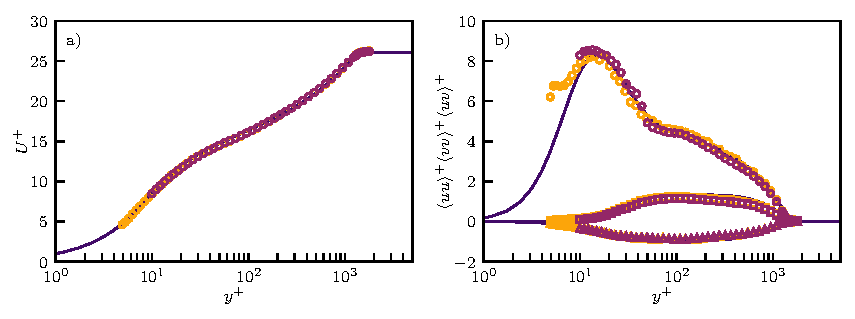
\includegraphics[width=\textwidth]{Figures/figure04.pdf}
    \caption{Profiles of the inner-scaled (a) mean velocity, and (b) Reynolds stresses of the velocity fluctuations. Colours refer to DNS \lcap{-}{dark}, EPTV - LR \lcap{-}{orange}, and EPTV - HR \lcap{-}{yellow}. In (b), symbols refer to streamwise \sy{black}{o}, wall-normal \sy{black}{s}, and shear \sy{black}{t} stresses.}
    \label{fig:F2_EPTVvsDNS}
\end{figure}


\subsection{Data processing}
A preprocessing is performed to remove the background and the laser reflection; the procedure is based on the eigenbackground subtraction described by \citet{Mendez2017181}. A super-resolution approach \citep{keane1995super} is followed to pair particle images in the captured dual-frames. The predictor velocity fields are obtained through image digital correlation \citep{willert1991digital}, based on a multi-pass \citep{soria1996investigation} image deformation algorithm \citep{scarano2001iterative} with a B-spline interpolation \citep{Astarita2005}. The final interrogation window is equal to 32 pixels with 75\% overlap region. Particle locations are identified with local maxima identification and Gaussian interpolation of the peak to achieve sub-pixel accuracy. The thresholding to identify whether a local maximum is a genuine peak is based on image statistics - only peaks above the local mean intensity plus one standard deviation are retained in the process. Particle images are then paired using a Kd-tree algorithm \citep{Tagliasacchi2021} for efficient pairing, with search biased by the PIV predictor. 

\subsection{EPTV and data post-processing} \label{ss:EPTV}
The ensemble averaging of the EPTV process is carried out on rectangular windows, with width of $200$ pixels and height variable between $3$ and $32$ pixels. A preliminary inspection of the wall reflection on the image allows to identify any misalignment between the camera reference system and the wall, and rotate the velocity vectors and averaging bins accordingly. Since the typical error in identifying manually the wall-position is of the order of the pixel size, the uncertainty of this procedure is below 0.5 degree.

On the streamwise direction an overlap of $80\%$ between the averaging windows is adopted. In the wall-normal direction initially a logarithmic grid has been adopted, with $50$ points from $1$ pixel above the wall up to $300$ pixels from the top of the image. In the last $300$ pixels a linear spacing has been adopted to obtain a robust estimate of the freestream. The profiles to be fitted with the composite profile are computed by averaging in the streamwise direction. A preliminary computation of the statistics has been carried out with the composite profile on the cases with window of $200\times3$ pixels (from now on named the reference cases for the LR and HR datasets using the full set of 28000 images). The results for the reference TBL are reported in Table~\ref{tab:1}. Additionally, the experimental reference cases are depicted in Figure~\ref{fig:fig01} against DNS data. 

The data are interpolated on a common grid based on the estimated $Re_\tau$ and wall position. The common grid is based on 70 logarithmically-spaced points from 0.1 wall units to {$0.9Re_\tau$},
and 20 linearly-spaced points from $0.93\delta$ to $1.3\delta$. This ensures that effects due to grid differences between the two datasets are removed.

The statistics computation is carried out by straightforward extraction of the statistical moments with equal weights on all vectors within the bin. While the polynomial approach by \citet{aguera2016ensemble} will improve the results close to the wall, it would not be comparable with the uncertainty estimation method presented in the previous section. Since the object of this work is to demonstrate the capability of our method to predict the uncertainty of the turbulent boundary layer parameters, we leave this aspect for future investigation.


\begin{figure}
    \centering
    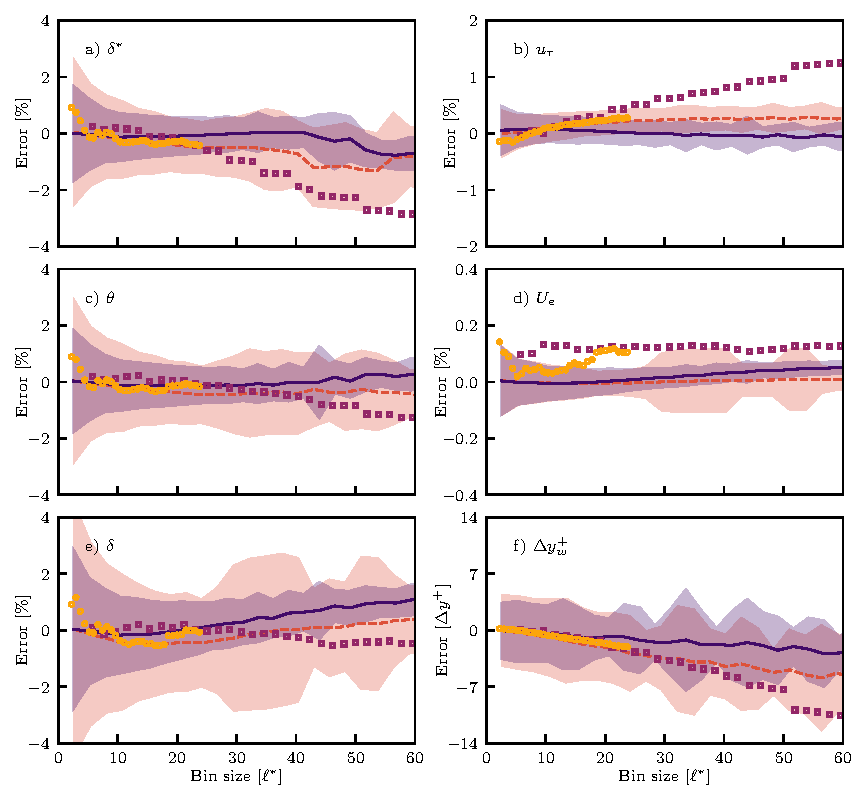
\includegraphics[width=\textwidth]{Figures/figure11.pdf}
    \caption{Comparison of error with respect to window size for a) displacement thickness, b) friction velocity, c) momentum thickness, d) freestream velocity, e) boundary layer thickness, and f) y origin. Symbols refer to DNS \lcap{-}{dark}, {Composite-profile} \lcap{--}{purple}, EPTV - LR \sy{orange}{s}, and EPTV - HR \sy{yellow}{o}. Error bars in DNS and {Composite-profile} refer to 3$\sigma$.}
    \label{fig:fig01}
\end{figure}


\subsection{Results}
\label{ss:expresults}

To compare the results among the experimental and the synthetic cases, the calculation of the profiles for the synthetic profiles has been carried out by setting the same resolution of the experiments. The averaged profiles are interpolated in the common grid described in \S\ref{ss:EPTV} to ensure the elimination of error sources due to grid differences between experimental and synthetic data.
Additionally, the estimation of TBL parameters is now performed by adding the random errors to the velocity profile and the {wall-normal} component. A total of 2000 runs are performed, and the standard deviation for each computed parameter is quantified to determine the corresponding uncertainty bars. 

The random error due to convergence is introduced as described in \S.\ref{ss:synthetic_method}, according to Eq.~\ref{ruido}. The TBL parameters are then computed using 2000 and 5000 images for the LR and HR dataset. The number of vectors $N_v$ is set equal to $350\cdot w$, with $w$ being the averaging bin size, to match the number of vectors observed in the dataset. The error of the experimental data is then estimated by using as a reference the velocity profile obtained using the full dataset of 28.000 images with window size of $200\times3$ pixels.

In Figure \ref{fig:F2_EPTVvsDNS} a comparison among the two experimental cases described in \S\ref{s:validation} and the DNS profile used as synthetic data is shown. Both experimental cases show an excellent agreement not only in the mean streamwise velocity profile (Figure \ref{fig:F2_EPTVvsDNS}a) but also in the different Reynolds stress components  (Figure \ref{fig:F2_EPTVvsDNS}b) up to the near-wall peak. For the high-resolution EPTV case, a deviation in the inner peak is appreciated which can be attributed to the residual reflections on the experimental images \citep{SanmiguelVila2017}. 

Figure \ref{fig:fig01} shows the relative error in the different boundary-layer parameters as a function of the bin size expressed in inner units. To normalise the error contribution, the resulting values of the {boundary-layer} quantities after fitting the original DNS profile, the Chauhan composite profile and the mean velocity profiles calculated using the full image data dataset (28.000 images) are employed. For the case of the quantities obtained by means of the composite profile proposed by \citet{Chauhan:2009p10824}, $u_\tau$ and $\Delta y^+$, it is observed for both quantities an error behaviour which, as expected, is equivalent to the error curves observed when analysing the effect of the first $y_0^+$ point available in hot-wire measurements \citep{Chauhan:2009p10824,Orlu:2010p36071,Rodriguez-Lopez2015}. For bin size values up to $\approx 12^+$, the error in both quantities is relatively small compared with the reference employed which is associated with profiles that have a $y_0^+<10$. When this bin size is exceeded, the error for both experimental cases shows much larger values. This effect is probably related to the higher levels of error in the logarithmic region for the experimental cases compared to the synthetic cases{, i.e. due to the strong local velocity profile curvature the PIV predictor for particles pairing is more prone to error}. For the quantities obtained by using the composite profile of \citet{Nickels:2004p15662} $\delta$, $U_e$, $\delta^*$ and $\theta$, the error curves are more robust and the agreement between the experimental data and the synthetic data is observed up to a bin size value of $\approx 25^+$. This corresponds to the location where there is no more inner points available and therefore all the estimation is performed based on the buffer and logarithmic region. It has to be noted that $U_e$ is slightly shifted in the error curves with respect to the reference. %As a consequence of the large number of images employed in the reference case (28.000), a more converged $U_e$ value is obtained compared to the error points which are calculated with only 2.000 images and therefore are more likely to be affected by the freestream disturbances.
This systematic error is quite small and might be to other minor issues, such as small drift of the flow conditions over the test time.

\section{Conclusions}

A method to estimate the uncertainty of {ZPG-}TBL parameters with the composite-profile based on data from full-field EPTV has been assessed. The proposed method is based on using data from simulations or composite profiles to reproduce the errors due to {wall-position} identification uncertainty, finite spatial resolution due to bin averaging and convergence due to finite number of samples. The synthetic and experimental validation demonstrate that the errors and uncertainty estimated using high-fidelity simulations and the composite-profile formulation are in good agreement, and predict accurately the range of error to be expected in the corresponding experiments. Simulation data can be more precise in determining the convergence limits since the streamwise velocity variance profile is well defined; on the other hand the approach based on the composite profile is more flexible, since it guarantees the possibility to closely match all the experimental conditions, including the Reynolds number.

The proposed approach can be used to:
\begin{enumerate}
    \item investigate systematic errors (as in \S\ref{s:SyntheticValidation}) by reproducing the same conditions to be expected in the experiments in terms of resolution and window size. It can be thus a useful tool to identify the requirements in terms of imaging before the experiments, and in principle it could also be used to reduce systematic errors.
    \item estimate the uncertainty range for the ZPG-TBL parameters. In this case, in addition to the spatial resolution and window size, the number of vectors per bin should also be included in the analysis to address errors due to convergence of the statistics. In this sense, this approach can be used also as an \textit{a priori} inference of the uncertainty, thus being useful to relate it quantitatively with the bin size and the number of vectors contained in it.
\end{enumerate}

\noindent{}It has to be remarked that this study is not including other sources of uncertainty which might be larger in an experiment than those quantified here, such as, for example, the uncertainty on the optical magnification. Furthermore, any departure from the condition of well-behaved ZPG TBL will determine additional uncertainty related to the suitability of the composite profile to fit the velocity profile. This is particularly delicate for quantities that are more sensitive to the quality of the near-wall region, such as $u_\tau$ or the wall position. 
Nonetheless, if any independent assessment of such additional uncertainty is available, the outcome of the uncertainty estimation approach proposed here can be used as input for the computation of combined uncertainties. \\

\section*{Code availability}
{The MATLAB\textregistered  codes for the calculation and plotting of the presented results are available from the repository \url{github.com/eaplab/EPTVuncertainty.git}. Camera-ready version of the figures have been generated with \url{github.com/guemesturb/TheArtist.git}.}

\section*{Acknowledgements}
RC, CSV and SD were partially supported by the Grant DPI2016-79401-R funded by the Spanish State Research Agency (SRA) and European Regional Development Fund (ERDF).


%------------------------------------------------------------------------------
% Bibliography
%------------------------------------------------------------------------------
%
%\clearpage
\bibliographystyle{jfm}
\bibliography{paper1/bib1}
%
\IfFileExists{paper1/bib1.bbl}{\input{paper1/bib1.bbl}}{}

%===============================================================================
%                            END PAPER
%===============================================================================
\end{paper}

%-------------------------------------------------------------------------------
% Paper 4: LGPC vs RL
%------------------------------------------------------------------------------
% Define title, author(s), affiliation and publishing status
%
\papertitle[ML flow control with few sensor feedback and measurement noise] % Short title used in healines (optional)
{%
Machine learning flow control with few sensor feedback and measurement noise% THE COMMENT SYMBOL AT THE END OF THIS LINE IS NEEDED
}%
%
\papertoctitle{Machine learning flow control with few sensor feedback and measurement noise} % Title for toc
%
\paperauthor[R. Castellanos \etal] % Short authors used in headlines and List Of Papers
{%
  Rodrigo Castellanos$^{1,2}$, Guy Y. Cornejo-Maceda$^{3}$, Ignacio de la Fuente$^{1}$ , Bernd R. Noack$^{3,4}$, Andrea Ianiro$^1$ \& Stefano Discetti$^{1}$%
}%
%
\listpaperauthor{Castellanos, R., Cornejo-Maceda, G. Y., de la Fuente, I., Noack, B. R., Ianiro, I. \& Discetti, S.}% (optional) Short authors used in List Of Papers
%
\paperaffiliation
{%
  $^1$ Aerospace Engineering Research Group, Universidad Carlos III de Madrid, Legan\'{e}s 28911, Spain\\%
  $^2$ Theoretical and Computational Aerodynamics Branch, Flight Physics Department, Spanish National Institute for Aerospace Technology (INTA), Torrej\'on de Ardoz 28850, Spain. \\%
  $^3$ School of Mechanical Engineering and Automation, Harbin Institute of Technology (Shenzhen),  University Town, Xili, Shenzhen 518055, People’s Republic of China \\%
  $^4$ Institut für Strömungsmechanik und Technische Akustik (ISTA), Technische Universität Berlin, Müller-Breslau-Straße 8, D-10623 Berlin, Germany
}%
%
\paperjournal[Phys. Fluids] % Short publish info used in List Of Papers
{%
	Physics of Fluids%
}%
%
\papervolume{34}%
%
\papernumber{4}
%
\paperpages{047118}%
%
\paperyear{2022}%
%
\papersummary%
{% Insert summary of the paper here (used in introduction)
A comparative assessment of machine learning (ML) methods for active flow control is performed. The chosen benchmark problem is the drag reduction of a two-dimensional Kármán vortex street past a circular cylinder at a low Reynolds number ($Re=100$). 
The flow is manipulated with two blowing/suction actuators on the upper and lower side of a cylinder. The feedback employs several velocity sensors. Two probe configurations are evaluated: 5 and 11 velocity probes located at different points around the cylinder and in the wake. 
The control laws are optimized with Deep Reinforcement Learning (DRL) and Linear Genetic Programming Control (LGPC). 
By interacting with the unsteady wake, both methods successfully stabilize the vortex alley and effectively reduce drag while using small mass flow rates for the actuation. DRL has shown higher robustness with respect to variable initial conditions and to noise contamination of the sensor data; on the other hand, LGPC is able to identify compact and interpretable control laws, which only use a subset of sensors, thus allowing reducing the system complexity with reasonably good results. 
Our study points at directions of future machine learning control combining desirable features of different approaches.
}
%
\graphicspath{{paper3/}}%
%
%
%===============================================================================
%                            BEGIN PAPER
%===============================================================================
%
\begin{paper}

\makepapertitle

%------------------------------------------------------------------------------
% Abstract
%------------------------------------------------------------------------------
%
\begin{paperabstract}
A comparative assessment of machine learning (ML) methods for active flow control is performed. The chosen benchmark problem is the drag reduction of a two-dimensional Kármán vortex street past a circular cylinder at a low Reynolds number ($Re=100$). 
The flow is manipulated with two blowing/suction actuators on the upper and lower side of a cylinder. The feedback employs several velocity sensors. Two probe configurations are evaluated: 5 and 11 velocity probes located at different points around the cylinder and in the wake. 
The control laws are optimized with Deep Reinforcement Learning (DRL) and Linear Genetic Programming Control (LGPC). 
By interacting with the unsteady wake, both methods successfully stabilize the vortex alley and effectively reduce drag while using small mass flow rates for the actuation. DRL has shown higher robustness with respect to variable initial conditions and to noise contamination of the sensor data; on the other hand, LGPC is able to identify compact and interpretable control laws, which only use a subset of sensors, thus allowing reducing the system complexity with reasonably good results. 
Our study points at directions of future machine learning control combining desirable features of different approaches.

        \keywords{Machine Learning, Deep Reinforcement Learning, Linear Genetic Programming,  Flow Control, Drag Reduction}
\end{paperabstract}


%------------------------------------------------------------------------------
% Article
%------------------------------------------------------------------------------
%
%%%%%%%%%%%%%%%%%%%%%%%%%%%%%%%%%%%%%%%%%%%%%%%
\definecolor{black}{RGB}{0, 0, 0}
\definecolor{blackR}{RGB}{25.5, 25.5, 25.5}
\definecolor{greyR}{RGB}{102, 102, 102}
\definecolor{redR}{RGB}{227, 47.3333, 39}
\definecolor{redRr}{RGB}{246, 191, 189}
\definecolor{greenR}{RGB}{55, 160.3333, 85}
\definecolor{greenRr}{RGB}{194, 225, 203}
\definecolor{blueR}{RGB}{55, 135, 192.3333}
\definecolor{blueRr}{RGB}{194, 218, 235}
%%%%%%%%%%%%%%%%%%%%%%%%%%%%%%%%%%%%%%%%%%%%%%

%%%%%%%%%%%%%%%%%%%%%%%%%%%%%%%%%%%%%%%%%%%%%%%%%%%%%%%%%%%%%%%%%%%%%%%%%%%%%%%
%%%%%%%%%%%%%%%%%%%%%%%%%%%%%%% INTRODUCTION %%%%%%%%%%%%%%%%%%%%%%%%%%%%%%%%%%
%%%%%%%%%%%%%%%%%%%%%%%%%%%%%%%%%%%%%%%%%%%%%%%%%%%%%%%%%%%%%%%%%%%%%%%%%%%%%%%
\section{Introduction}\label{s:Introduction}

%%%%%% Research interest
Flow control of turbulent flows, in particular with the purpose of drag reduction, is a recurrent research objective that has regained interest during the last decade \citep{Noack2019control}. Machine learning, in particular, plays a key role in the development of sophisticated and efficient flow-control algorithms \citep{BruntonNoackKoumoutsakos2020} and presents a possible solution to the difficulties imposed by the non-linearity, time-dependence, and high dimensionality inherent to the Navier-Stokes equations.

%%%%%% Wake flow and relationship to drag
Control of wake flows, in particular, has attracted significant interest due to its relevance in a wide variety of research and industrial applications. Control strategies commonly target two main types of drag: the skin friction drag, caused due to the viscosity of the fluid interacting with the wall surface, and the wake drag, which originates after the affected body.

Passive drag reduction methods, such as the classical dimples on the surface of a sphere \citep{Bearman1993dimples} to delay transition or the use of splitter plates in the wake \citep{Ozono1999splitter} to suppress the vortex shedding, have shown to be quite successful. Nonetheless, during these last decades, hardware/software advances are pushing towards active methods instead, which exploit the potential advantage of tuning the action according to the flow state. 

Active drag reduction techniques initially focused on increasing base pressure to reduce pressure drag, using transpiration and vibration techniques for such an objective. Continuous or pulsating-based-bleeds could be used to modify the flow in the separated region. For the latter, drag reduction could be achieved with zero net mass addition, with maximum effectiveness at a frequency twice the K\'arm\'an shedding frequency \citep{Williams1989}. Among the wide variety of active drag reduction techniques that resulted effectively, small jets have shown to be very efficient, enabling separation control with weak actuation \citep{glezer2011control}. 

%% flow control as optimization problem
The design of effective flow control techniques is a challenging objective, especially when the solution is based only on limited velocity or pressure data extracted from the fluid flow \citep{duriez2017book}. In its essence, the flow control problem can be described as a functional optimization problem, in which the state of the dynamical system has to be inferred from a limited number of observable quantities. The objective is to find a control function that minimizes (or maximizes) a cost (or reward) function, based on the desired features for the controlled flow configuration.

%% Control categorization (model-based and model-free), and introduction of GP and RL
Considering the categorization of control strategies, one of the main classifications is based on the existence of a model to describe the system to be controlled, distinguishing between model-based and model-free control. The latter encloses the kind of control strategies where an optimized control law is extracted without imposing any model of the dynamical system. The popularity of these approaches has been growing considerably in the last decade, thanks to the popularization and advances in machine learning techniques. Two of the most prominent model-free control techniques from the machine learning literature are Reinforcement Learning \citep[RL]{sutton2018reinforcement} and Genetic Programming \citep[GP]{koza1994}. Reinforcement Learning is an unsupervised learning technique focused on optimizing a decision-making process interactively, which makes it a preferred choice in flow control over its alternatives. On the other hand, Genetic Programming algorithms are focused on recombining good control policies by systematic testing, exploiting the ones with the best results and exploring possible alternatives in the solution space. 

%%%%%% GP description and approaches
Genetic Programming, originally pioneered by \citet{koza1994} belongs to the family of Evolutionary Algorithms (EA), which have a common workaround: a population of individuals, called a generation, compete at a given task with a well-defined cost function, and evolve based on a set of rules, promoting the most successful strategies to the next generation \citep{banzhaf1998genetic, duriez2017book}. It constitutes a powerful regression technique able to re-discover and combine flow control strategies, which have been proven useful in the cases of multi-frequency forcing, direct feedback control and controls based on ARMAX (Autoregressive Moving Average eXogenous), without any physics information \citep{cornejomaceda2019pamm,cornejo2021gMLC}. 
Machine Learning Control (MLC)\citep{duriez2017book} based on tree-based Genetic Programming has been able to develop laws from small to moderate complexity, e.g. the phasor control, threshold-level based control, periodic or multi-frequency forcing, including jet mixing optimization with multiple independently unsteady minijets placed upstream of nozzle exit \citep{zhou2020artificial}, the analysis of the effect of a single unsteady minijet for control \citep{Wu2018jet}, drag reduction past bluff bodies \citep{li2019prf} , shear flow separation control \citep{gautier2015MLC}, reduction of vortex-induced vibrations of a cylinder \citep{Ren2019pof}, mixing layer control \citep{Parezanovic2016jfm}, and wake stabilization of complex shedding flows \citep{raibaudo2019pof} among others.
Some relevant improvements have been made to the MLC framework  such as the integration of a Linear-based Genetic Programming (LGP) algorithm \citep{li2017GP}, which is the chosen option in this study. Recently, a faster version of MLC based on the addition of intermediate gradient-descent steps between the generations (gMLC) has been developed \citep{cornejo2021gMLC}


%%%%%% RL description and approaches
Reinforcement Learning is based on an agent learning an optimized policy based on the different inputs and outputs. The key feature of RL is that the only information available for the algorithm is given in the form of a penalty/reward concerning a certain action performed by the model, but no prior information is available on the best action to take. In Deep RL (DRL), the agent is modelled by an Artificial Neural Network (ANN) which needs to be trained \citep{rabault2019DRL}. ANN  have a long history of use to parametrize control laws \citep{Lee1997NN}, or to find the optimized flow control strategy for several problems such as swimming of fish schoolings \citep{gazzola2014RL}, control of unmanned aerial vehicles \citep{bohn2019DRL}, and optimization of glider trajectory taking ascendance \citep{reddy_learning_2016}. On the other hand, the exploitation of DRL specifically on flow control is relatively recent. The first applications targeted the control of the shedding wake of a cylinder in simulations \citep{rabault2019DRL,rabault2019JFM} and in experiments \citep{Fan2020}. 
DRL has been enforced in tuning the heat transport in a two-dimensional Rayleigh–Benard convection \citep{Beintema2020}, in the control of the the interface of unsteady liquid films \citep{Belus2019} and in stabilizing the wake past a cylinder by imposing a rotation on two control cylinders located at both sides \citep{Xu2020joh}. 
Recently, \citet{li2021ReLe} investigated how to use and embed physical information of the flow in the DRL control of the wake of a confined cylinder, and \citet{paris2021} explored the utilization of DRL for optimal sensor layout to control the flow past a cylinder.

It can be argued that LGP and DRL share many similarities, up to the point in which many fitness functions in LGP can be considered as DRL systems\citep{banzhaf1998genetic}. The recent ongoing developments of DRL and LGP in flow control applications open up relevant questions on their applicability in experimental environments, where the number of sensors is limited and data are likely to be corrupted by noise. Furthermore, the generalization of the identified policies is often hindered by the challenges of interpreting the control laws. This work sheds light on the main features of Deep Reinforcement Learning as Linear Genetic Programming Control (LGPC) in this direction. To the author's best knowledge, only the recent contribution by \citet{pino2022comparative} performs a comparative assessment of machine learning methods for flow control. The work focuses on the comparison of the relation of DRL and LGPC with optimal control for a reduced set of sensors. The robustness to noise and the effect of initial condition of such algorithms is not discussed. The present study aims to address the performance of DRL and LGPC in the simple scenario of the control of the 2D shedding wake of a cylinder at a low Reynolds number in the conditions of a limited number of sensors. The robustness of both processes to noise contamination on the sensor data and variable initial conditions for training individuals is assessed. Finally, an interpretation of the control actions using a cluster-based technique is provided. For this purpose, the same DRL framework and simulation environment used by \citet{rabault2019DRL} is considered, and compared against the LGPC environment developed by \citet{li2017GP}.
It is to be noted that this contribution is a proof of concept. The simulation environment proposed by \citet{rabault2019DRL} was chosen given its simplicity and affordability for extensive analysis as herein presented. Nonetheless, the application of akin algorithms to similar environments, though with more challenging conditions, was investigated by \citet{Tang2020pof}, achieving a robust control in the flow past the confined cylinder at multiple Reynolds numbers, concluding that the drag reduction increases with the Reynolds number. Additionally, \citet{Ren2021pof} exploits the framework by \citet{rabault2019DRL} at weak turbulent conditions (Re = 1000) with a drag reduction of 30\%. Nonetheless, in these studies, 236 and 151 probes are considered respectively, and the robustness to noise is not explored.

The present article is structured as follows: Section \ref{s:Methodology} defines the main methodologies applied to implement the different machine learning models, the simulation environment and the problem description. Results are collected and described in Section \ref{s:result} while the interpretation of the achieved controls and their performance is outlined in Section~\ref{s:interpretability}. Ultimately, the conclusions of the study are drawn in Section \ref{s:Conclusions}.

%%%%%%%%%%%%%%%%%%%%%%%%%%%%%%%%%%%%%%%%%%%%%%%%%%%%%%%%%%%%%%%%%%%%%%%%%%%%%%%
%%%%%%%%%%%%%%%%%%%%%%%%%%%%%%% METHODOLOGY %%%%%%%%%%%%%%%%%%%%%%%%%%%%%%%%%%%
%%%%%%%%%%%%%%%%%%%%%%%%%%%%%%%%%%%%%%%%%%%%%%%%%%%%%%%%%%%%%%%%%%%%%%%%%%%%%%%
\section{Methodology}\label{s:Methodology}

This Section is focused on the main methodologies to define the environments in which the Machine Learning models will be tested, as well as the conditions imposed. Although the methodologies to be compared present important differences, they share several fundamental characteristics that must be highlighted before delving into each of the independent methods.

\begin{figure}[t]
    \centering
    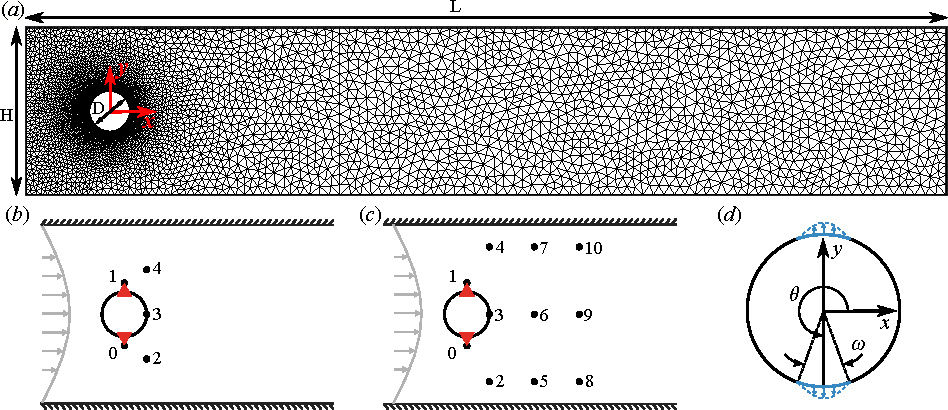
\includegraphics[width=0.99\linewidth]{Figures/1.pdf}
    \caption{Description of the numerical setup adapted from \citet{rabault2019JFM}. (a) Sketch of the numerical domain and the non-structured mesh, defining the diameter $D=1$, length $L=20$, and height $H=4.1$. The sensor arrangement is shown for (b) 5 and (c) 11 probes, being probes identified as \sy{black}{o*} and actuators as \sy{redR}{t*}. (d) Detail of the cylinder and the jet actuators definition.}
    \label{fig:NumericalSetup}
\end{figure}

\subsection{Simulation Environment}

The active drag reduction is performed in a 2D Direct Numerical Simulation (DNS) environment that builds upon that of \citet{rabault2019JFM}, differing only for the sensor strategy. The environment is described here for completeness. 

The geometry of the simulation, adapted from state of the art benchmarks \citep{schafer_benchmark_1996}, consists of a cylinder of diameter $D$ immersed in a box of total length $L=22D$ (along the $x$-axis) and height $H=4.1D$ (along the $y$-axis) as shown in figure~\ref{fig:NumericalSetup}(a). The inflow velocity (on the left wall of the domain) is modelled as a parabolic profile so that the mean velocity magnitude results in $U$.
A no-slip boundary condition is imposed on the top and bottom walls of the channel, and also on the solid cylinder walls. An outflow Dirichlet boundary condition is imposed on the right wall of the domain. The Reynolds number based on the mean velocity magnitude and cylinder diameter ($Re=\frac{{U} D}{\nu}$, with $\nu$ the kinematic viscosity) is set to $Re=100$. This choice is based on the previous work by \citet{rabault2019JFM} which has been a pioneer application
of DRL to flow control and the baseline to compare within this study. Working with higher Reynolds numbers would have implied a tremendous increase in computational cost, making unaffordable all the set of simulations required for changing the initial conditions and assessing the noise robustness that will be discussed in the following.

The control action is performed by two jets (1 and 2) controlled through a non-dimensional mass flow rate $Q_{\rm jet}$ by imposing a parabolic velocity profile with the jet width of $\omega = 10^\circ$. The jets are perpendicular to the cylinder wall and located at angles $\theta_1 = 90^\circ$ and $\theta_2 = 270^\circ$ relative to the flow direction as shown in figure~\ref{fig:NumericalSetup}(d), what guarantees that all the promoted drag reduction is the result of indirect flow control, rather than direct injection of momentum~\citep{rabault2019JFM} To prevent numerical instability while presenting a more realistic scenario, the total mass flow rate injected by the jets is zero, i.e. $Q_{\rm jet_1} = -Q_{\rm jet_2}$. Note, however, that the cylinder does not present physical cavities on its surface, meaning that there is no physical interference of the jet slot with the flow field.

The simulation environment is based on the open-source finite-element framework FEniCS \citep{logg2012book} version 2017.2.0, solving the unsteady Navier–Stokes equations equations by DNS.  Computations are performed on an unstructured mesh generated with Gmsh \citep{geuzaine2009gmsh}. The mesh is refined around the cylinder and is composed of $9262$ triangular elements (see figure~\ref{fig:NumericalSetup}(a)). A non-dimensional, constant numerical time step $dt=5 \times 10^{-3}$ is used. The CFL condition is enforced in the problematic zones, that is, close to the actuation jets, by imposing a maximum jet mass flow rate ($|Q_{\rm jet}|<Q_{\rm jet_{max}}$). %0.06 \citep{rabault2019JFM}.

The flow control framework developed by \citet{rabault2019JFM} was conceived to work either with velocity or pressure probes as sensing. Since pressure probes are often more difficult to be installed in a customary location for an experimental application, it was preferred to chose the velocity probes which resembles what could be extracted from hot wire anemometry (HWA). Two sensor configurations are considered in the present study with $5$ and $11$ probes which report the local value of the horizontal and vertical components of the velocity field (see figure~\ref{fig:NumericalSetup}(b) and \ref{fig:NumericalSetup}(c), respectively). The probes are located in the wake of the cylinder to enable the controller to learn from the vortex shedding pattern.

\subsection{Formulation of the optimization problem}

\begin{figure}
    \centering
    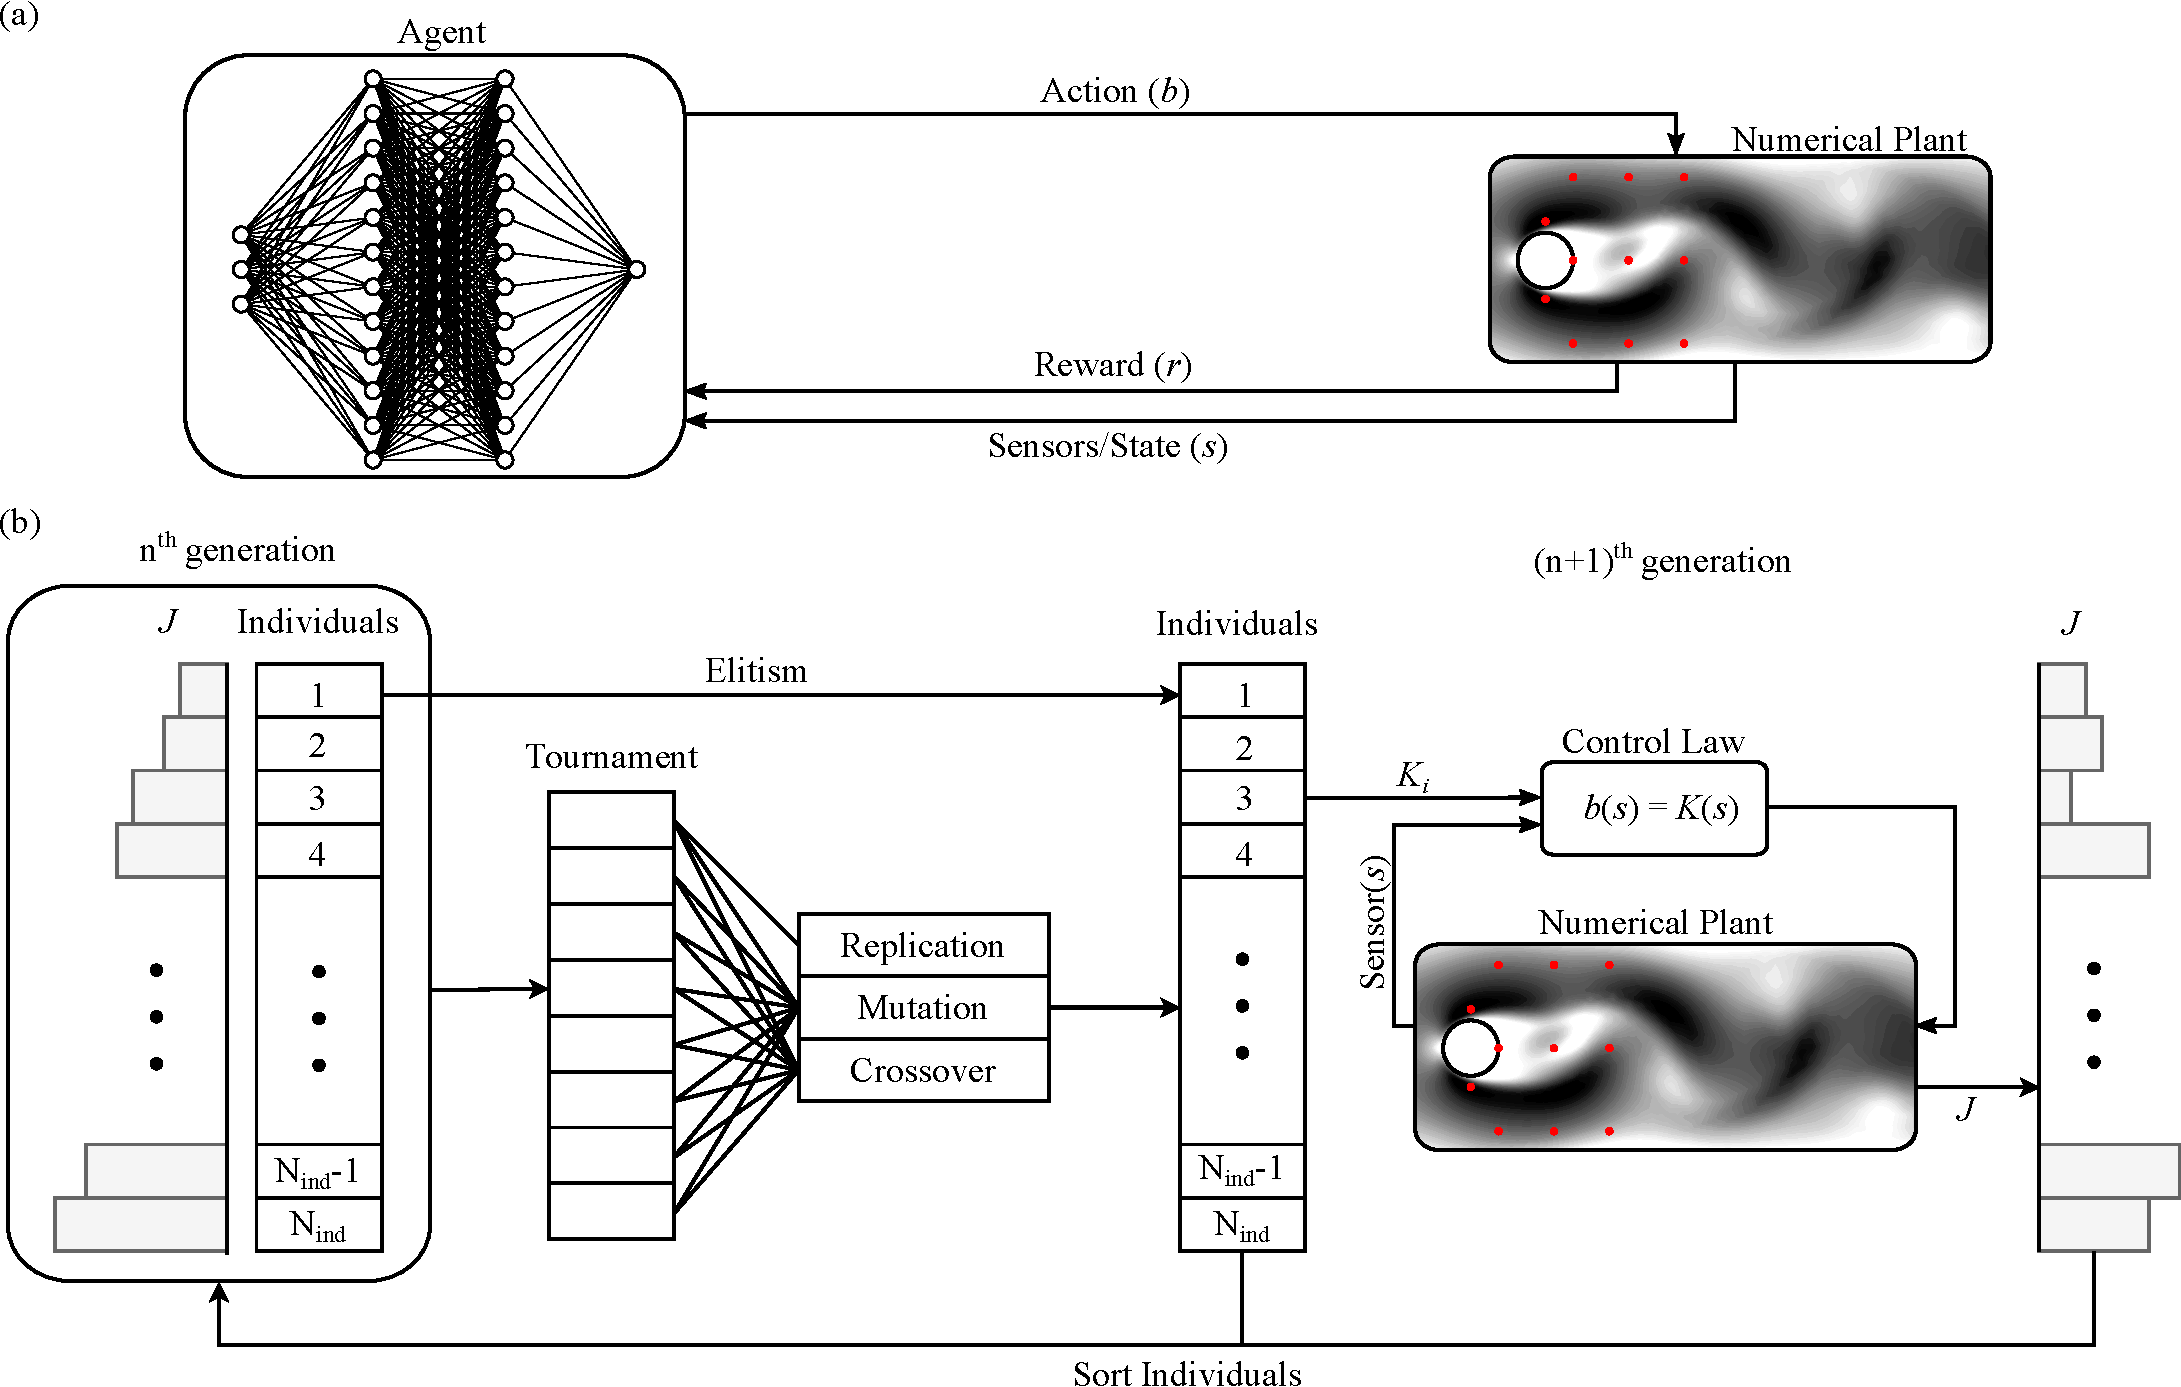
\includegraphics[width=0.99\linewidth]{Figures/2.pdf}
    \caption{Implementation of the control algorithms. (a) Sketch of the closed-loop control based on Deep Reinforcement Learning. (b) Sketch of the closed-loop control based on Linear genetic Programming.}
    \label{fig:LearningLoop}
\end{figure}

The drag reduction of a 2D cylinder wake flow is a classical optimization problem with a simple target, i.e. reducing drag. The control problem is formulated as a regression problem, i.e. to find the control law which optimizes a given cost function $J$ \citep{duriez2017book}. The proposed cost function has been shaped as a combination of drag and lift coefficients, modifying the one proposed by \citet{rabault2019JFM} as follows:

\begin{equation}
    J= 1+\left\langle C_{D}\right\rangle_{T} - \left\langle C_{D_0}\right\rangle_{T}+0.2\left|\left\langle C_{L}\right\rangle_{T}\right| \label{Eq:J}
\end{equation}

where $\langle C_{D_0}\rangle_T = 3.206$ is the drag coefficient of the unforced flow, and $\langle \cdot \rangle_T$ indicates the sliding average back in time over a duration corresponding to one vortex shedding cycle $T$ of the unforced vortex shedding flow. 

The cost function in equation~\ref{Eq:J} has shown to be better than using just the instantaneous drag coefficient, i.e. $J(t) = C_D(t)$. First, the average values of the lift and drag coefficients over one vortex shedding cycle reduce the oscillations of the objective function, which has been reported to improve learning speed and stability \citep{rabault2019JFM}. Secondly, the drag reduction is defined as the increment with respect to the unforced flow ($\Delta C_D = \left\langle C_{D}\right\rangle_{T} - \left\langle C_{D_0}\right\rangle_{T}$), which is intended to be as negative as possible. Thirdly, a penalization term based on the lift coefficient is considered to prevent the controller from finding undesired asymmetric solutions\citep{rabault2019JFM}. Finally, adding the unity to the cost function provides a bias to prevent $J$ negative values that could affect the convergence of the learning process. Ultimately, the algorithm would try to minimise $J$, by reducing drag while maintaining low lift components.

From an optimization perspective, the resultant control is the strategy that minimizes the cost function with a control law $\bm{b}(t) = {K}(\bm{s}(t))$, where $\bm{b}(t) = (b_1(t), ...,b_{N_b}(t))^T$ comprises $N_b$ actuation commands, and $\bm{s}(t) = (s_1(t), ..., s_{N_s}(t))^T$ consist of $N_s$ sensor signals. In this study, the actuation $b$ is performed with two jets that are related due to the net zero flux condition ($N_b = 1$) at the bottom and top sides of the cylinder, using velocity probes ($N_s = 5$ or $11$) as sensing. The control problem is equivalent to finding ${K}^{*}$ such that
\begin{equation}\label{eq:Optproblem}
    \begin{aligned}
        {K}^{*}(\bm{s}) = \underset{{K}}{\arg\min}~~ J({K}(\bm{s}))
    \end{aligned}
\end{equation}

The optimized feedback ${K}^{*}$ is computed following LGPC and DRL, as described in the following sections. The resultant control laws map $N_s$ sensor signals into $N_b$ actuation commands.
The resultant control action is subjected to a smoothing operation to ensure continuous control signals without abrupt alterations in the pressure and velocity due to the use of an incompressible solver. The control action is then adjusted from one-time step in the simulation to the next by
\begin{equation}\label{eq:Qsmooth}
    Q_{\rm jet}(t)=Q_{\rm jet}(t-dt)+\alpha\left[{b}(t)-Q_{\rm jet}(t-dt)\right],
\end{equation}
being $\alpha=0.1$ a numerical parameter, $Q_{\rm jet}(t)$ the jet actuation used by the plant at time instant $t$, and ${b}(t)$ the actuation proposed by the machine learning model at time instant $t$. 

%----------- DRL -------------------------------------------------------
\subsection{Deep Reinforcement Learning}

Deep Reinforcement Learning (DRL) is an ML control algorithm in which an agent (managed by an ANN) learns the best control by interacting with the environment to exchange information in a closed-loop process (see figure~\ref{fig:ApproxMethod}(b)). In the present work, the plant or environment is the above-mentioned simulation environment, which interacts with the agent by three channels: the observation or sensor state, $\bm{s}$ ($N_s$ point measurements of velocity); the action, $b$ ($N_b$ values of mass flow rate to impose on the jets); and the reward, $r$ (the cost function in equation \ref{Eq:J} based on $C_D$ and $C_L$, i.e. $r=J$). Based on the sensing data and the reward of the current state, DRL trains an ANN to find the optimized closed-loop control strategies that maximize the expected reward.

The DRL framework is the same as in \citet{rabault2019JFM} in which the agent uses the proximal policy optimization (PPO) method \citep{schulman_proximal_2017} for performing learning. The PPO method is episode-based, so that it iteratively learns by applying a certain control for a limited amount of time (episode duration) before analysing the rewards and sensors, and resuming learning with a new episode. The considered architecture for the ANN is relatively simple, being composed of two dense layers of $512$ fully-connected neurons, the input layer to acquire data from the probes, and the output layer to generate data for the two jets. For more details, readers are referred to \citet{rabault2019JFM}. The training loop of DRL is sketched in Figure \ref{fig:LearningLoop}(a).

At the beginning of the learning process, the PPO explores purely random controls to assess the values of the reward function. This initial approach implies difficulties to learn the necessity to set time-correlated, continuous control signals. To solve this issue, \citet{rabault2019JFM} implemented the agent such that the control value provided by the network is kept constant for a duration of $50$ numerical time steps. Therefore, the PPO agent interacts and updates the ANN coefficients only every $50$ time steps, which is the duration of a fixed actuation. This numerical trick together with the smoothing described in equation \ref{eq:Qsmooth} provides a continuous control signal. 


%----------- LGP ------------------------------------------------------
\subsection{Linear Genetic Programming}
Linear Genetic Programming \citep[]{Wahde2008book} is an evolutionary algorithm, that applies biological-inspired operations to select the fittest individuals for a given purpose. The control laws are effectively mappings between the outputs (sensor information) and the inputs (actuation) of a dynamical system. In the following, the control laws are also referred to as \textit{individuals} to comply with the evolutionary terminology. LGP is able to learn control laws in a model-free meaner, optimizing both the structure of the function and its parameters. In practice, the control laws are internally represented by a matrix encoding a list of instructions. Each row of the matrix codes for a mathematical operation from a set of input registers, constants and operations and stores the result in a memory register. The matrix is then read linearly modifying sequentially the memory registers, hence the name of the method. The control law is then read in the first register. LGPC is here selected as the preferred option for its simpler implementation of the genetic operators for Multiple-Input-Multiple-Output control \citep{cornejomacedaPhD}.

The learning process, sketched in Figure \ref{fig:LearningLoop}(b), is divided into an outer loop devoted to evolving the generations and an inner loop to evaluate all the individuals in a real-time control process. First, an initial population of individuals is randomly generated and evaluated with a Monte-Carlo optimization to explore the control law space. We recall that the individuals are analytical functions of the input data, i.e. the velocity sensor signals. A measure of the performance of each individual is given by its cost $J$ (equation~\ref{Eq:J}). Once the entire population is evaluated, the next generation of individuals is created with genetic operators (crossover, mutation, replication) applied to the most performing individuals. The best individuals are selected with the tournament selection method. Crossover combines two individuals and generates a new pair of individuals by exchanging randomly their instructions. This operation contributes to the exploitation of the learned data by recombining well-performing individuals. The mutation operation modifies randomly elements of one given control law to explore potentially new and better minima. Replication is the memory operator. It assures that good structures are not lost in the evolution process. Finally, an elitism operation saves the best individuals of one generation to the next, ensuring that the performance does not degrade after each generation. The genetic operators (crossover, mutation and replication) are chosen following respective probabilities ($P_c,P_m,P_r$). The process is repeated for every new generation until the stopping criterion is met or if the termination is triggered. In this study, all the training processes have been performed for a fixed number of generations $N_{g} = 15$ as explained later.  

Among the wide variety of custom settings when dealing with LGPC, the most relevant parameters for proper performance and convergence of the algorithms are the population size, the number of generations, the tournament selection size and the genetic operators' probability ($P_c,P_m,P_r$). LGPC parameters are chosen following the recommendations of \citet{duriez2017book} and \citet{li2017GP}. They are summarized in table~\ref{tab:GAparameters}

\begin{table}[h]
    \centering
    \begin{tabular}{lc}
    \toprule
    Number of controllers                       & 1 \\
    Number of sensors                           & 5,11 \\
    Population size                             & 100 \\
    Number of generations                       & 15 \\ %midrule
    Tournament selection size                   & 7   \\ 
    Crossover probability                       & 0.6 \\ 
    Mutation probability                        & 0.3 \\
    Replication probability                     & 0.1 \\
    Elitism                                     & 1   \\
    Operations                                  & $+$, $-$, $\times$, $\div$, $\sin$, $\cos$, $\tanh$ \\ \bottomrule
    \end{tabular}
    \caption{Selection of LGPC parameters} \label{tab:GAparameters}
\end{table}

An important difference between the DRL and the LGPC algorithm is related to their learning process during an episode. In DRL, the agent builds its internal representation of how the flow in a given state will be affected by actuation, and how this will affect the reward value. This is done globally at the end of the episode and also each time the actuation changes. The agent is modified according to the expected reward (total or partial, respectively), which is not an immediate value just after the actuation, but also after the medium/long-term reward. This means that the neural network on which the DRL is capable of learning both from the committed errors but also from the future effect associated with each actuation. In LGPC, there is no chance of the actuation law during the simulation run, as it corresponds to a single individual mapping from the input to the outputs. It is therefore interesting considering the incorporation of time-delayed sensor signals. Following \citet{cornejo2021gMLC}, the values of the probes at $1/4, 1/2$ and $3/4$ of the shedding period are included, as well as the instantaneous value. Assuming a periodic flow, the addition of such time delays enables the reconstruction of the flow phase.

%----------- Standards --------------------------------------------------
\subsection{Training standards}
The training process of both DRL and LGPC is performed with the same parameters, which were chosen based on the recommendations by \citet{rabault2019JFM} and extensive empirical analysis. The duration of the simulation (or episode duration, according to DRL nomenclature) is set to $T_{sim} = 20.0$, which translates into approximately 6 vortex shedding periods, and corresponds to 4000 numerical time steps. Note, however, that the cost function in equation~\ref{Eq:J} is evaluated for the last shedding period (650 numerical time steps) in which a new steady state is expected to be reached upon actuation.

Regarding the action, the DRL agent adjusts the policy every $50$ numerical time steps, which means that the control is updated $80$ times during the episode. The transition from the current action to the updated following action is smooth and continuous based on the smoothing described in equation~\ref{eq:Qsmooth}. On the other hand, LGPC provides analytical control laws that are continuous and fully dependent on the sensing data, which means that the control action is adjusted every numerical time step mildly thanks to the smoothing.

Given the intrinsic differences between LGPC and DRL, it is required to set the training standard to guarantee a fair comparison. The followed criterion is to keep the same computational time during the training process. The PPO agent is able to learn a fully-stabilized control after approximately $400$ epochs (corresponding to $32000$ sample actions); however, the convergence rate is lower when applying noise to the probes. On the other hand, for LGPC with a pool size of $100$ individuals per generation, a converged control law is achieved before the $10^{th}$ generation both with and without noise consideration. Both for LGPC and DRL, it is straightforward to assess that the main computational cost comes from the plant, i.e. from the fluid mechanic simulation of the 2D cylinder wake. The evaluation of the sensing, update of the agent or generation of new individuals are operations with negligible time consumption. Based on these figures of merit, it was decided to set the training duration to $1500$ episodes in the case of DRL and $15$ generations of $100$ individuals in the case of LGPC. This common criterion guarantees that the computational effort is the same for both algorithms since a total of $1500$ simulations are launched for each method.

For the investigation of robustness to noise, a perturbation with Gaussian distribution is added to the probes such that the input used by the DRL agent or the LGPC control laws are altered. The noise implementation is the following,
\begin{equation}
    u_i(t) = u_i(t) + \varepsilon \cdot \digamma_i(t) \qquad \forall \quad i = [1,2, ... , N_b],
\end{equation}

being $u_i(t)$ the velocity value, $\digamma_i(t)$ a random normally distributed value for the probe $i$ at time instant $t$, and $\varepsilon$ the noise level or intensity. Three noise levels are considered, i.e. $1\%,5\%$ and $10\%$ of the freestream velocity. On the contrary, the mean state quantities used to compute the cost function (i.e., $C_D$ and $C_L$) are not altered by noise since the averaging operator in the cost function would make the noise of minor relevance. 

\subsection{Control law visualization}\label{Sec:Method_ControlLawVisu}
%
\begin{figure}
    \centering
    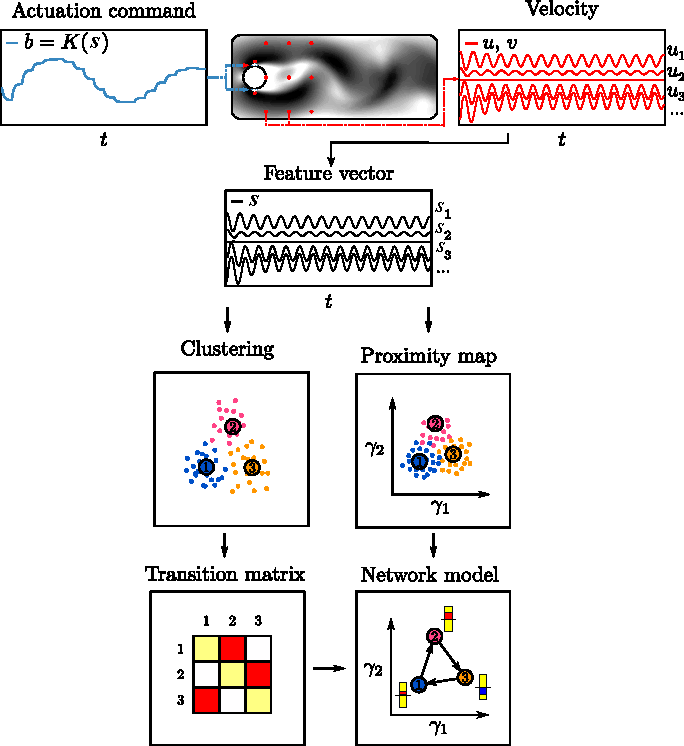
\includegraphics[width=0.75\linewidth]{Figures/3.pdf}
    \caption{Control interpretation methodology. The sensor vector is built from the vertical and horizontal components of the measured velocity. The elements of the sensor vector are grouped in clusters (three clusters (1,2,3) are presented here for clarity). High probability transitions are depicted with darker colours. $\gamma_1$ and $\gamma_2$ define the projection plane for the proximity map. The actuation magnitude is represented by rectangles in the network model; red (blue) for a positive (negative) actuation with respect to the mean value. See the text for more details.}
    \label{fig:ApproxMethod}
\end{figure}

A cluster-based interpretation method is considered to have an insight into the actuation mechanisms involved in the control learned by DRL and LGPC. Cluster-based methods have been recently applied to build network models able to reproduce the main characteristics of fluid flows and dynamical systems, such as temporal evolution and fluctuation levels \citep{Fernex2021,LiH2021jfm}.

Understanding the relationship between the control inputs and the corresponding actuation command is not an easy task, especially with a large number of inputs. Thus, clustering is employed to extract representative states from the sensors. Figure~\ref{fig:ApproxMethod} summarizes the main steps of the control interpretation methodology described below. For this study, the metric employed for the cluster analysis is the one induced by the $L^2$ norm. The sensor time series are reduced to $10$ clusters. For each cluster, its centroid is computed as the average of all states in the cluster. Then, the $10$ centroids represent the main states of the flow. Moreover, the transition information from one flow state to another is gathered in a probability transition matrix ($P=[p_{i,j}]_{i,j}$) that translates the probability to jump from one cluster to another. The probability transition from cluster $i$ to cluster $j$ is defined by $p_{i,j}={n_{i,j}}/{n_i}$, being $n_{i,j}$ the number of states from cluster $i$ that transition to cluster $j$ and $n_i$ the total number of states in cluster $i$.

The centroids combined with the transition matrix allow for building a network model of the controlled flow based only on the controller inputs. On the other hand, the sensor time series are projected on a 2D proximity map with classical multidimensional scaling \citep[MDS]{Kaiser2017ifac,LiA2022jfm,foroozan2021unsupervised}. MDS is a powerful tool for dimensionality reduction, that projects the data in the two directions ($\gamma_1$,$\gamma_2$) of maximum dispersion of the feature vector distance matrix. The distance matrix is computed with the same metric as the clustering. Combining the network model and the proximity map allows to have a reconstruction of the flow phase space. Finally, the average actuation performed in the cluster is associated with each centroid. The resulting 2D visualization represents the dynamics of the flow alongside the actuation performed allowing an easy interpretation of the control actuation mechanism.

%%%%%%%%%%%%%%%%%%%%%%%%%%%%%%%%%%%%%%%%%%%%%%%%%%%%%%%%%%%%%%%%%%%%%%%%%%%%%%%
%%%%%%%%%%%%%%%%%%%%%%%%%%%%%%% results %%%%%%%%%%%%%%%%%%%%%%%%%%%%%%%%%%%
%%%%%%%%%%%%%%%%%%%%%%%%%%%%%%%%%%%%%%%%%%%%%%%%%%%%%%%%%%%%%%%%%%%%%%%%%%%%%%%

\begin{table}[t]
\centering
%\begin{tabular}{>{\centering}p{0.125\linewidth-2\tabcolsep}
%                >{\centering}p{0.125\linewidth-2\tabcolsep}
%                >{\centering}p{0.125\linewidth-2\tabcolsep}
%                >{\centering}p{0.125\linewidth-2\tabcolsep}
%                >{\centering}p{0.125\linewidth-2\tabcolsep}
%                >{\centering}p{0.125\linewidth-2\tabcolsep}
%                >{\centering\arraybackslash}p{0.125\linewidth-2\tabcolsep}}
\begin{tabular}{ccccrrrr}
\toprule
Algoritm & Probes & Noise & $\langle J \rangle$ & $\langle C_D \rangle$ & $\langle C_L \rangle$       & std$(Q_{jet})$ \small{($\times 10^4)$} \\ \midrule
\multicolumn{3}{c}{-- No Control --}        & 1.160 & 3.206 &  0.022 &  0 \\ \midrule
DRL       & 5      & 0\%   & 0.992 & 3.085 & -0.207 &  5.744 \\
DRL       & 11     & 0\%   & 0.807 & 2.958 &  0.138 & 6.526 \\
DRL       & 11     & 1\%   & 0.808 & 2.961 & -0.095 &  6.3848 \\
DRL       & 11     & 5\%   & 0.811 & 2.961 &  0.001 & 8.828 \\
DRL       & 11     & 10\%  & 0.843 & 2.982 &  0.043 & 10.382 \\ \midrule
LGPC     & 5      & 0\%   & 0.966 & 3.065 & -0.271 & 10.225 \\
LGPC     & 11     & 0\%   & 0.846 & 2.954 &  0.058 & 20.285 \\
LGPC     & 11     & 1\%   & 0.797 & 2.946 & -0.129 & 12.912 \\
LGPC     & 11     & 5\%   & 0.984 & 2.997 &  0.233 & 24.446 \\
LGPC     & 11     & 10\%  & 0.901 & 2.984 &  0.155 & 12.246 \\ \bottomrule
\end{tabular}
\caption{Summary of results.}
\label{tab:SummaryResults}
\end{table}

\begin{table}[t]
\centering
%\begin{tabular}{>{\centering}p{0.08\linewidth-2\tabcolsep}
%                >{\centering}p{0.08\linewidth-2\tabcolsep}
%                >{\centering\arraybackslash}p{0.76\linewidth-2\tabcolsep}}
\resizebox{\textwidth}{!}{%
\begin{tabular}{ccc}
\toprule
Probes & Noise & Control Law ($Q_{jet} \times 10^2$)\\ \midrule
5 & 0\% &
$\begin{array}{c}  \sin\left(\tanh\left(\left( \tanh\left(\left(\left(\left( u_4\left(t-\frac{3T}{4}\right)+v_0\left(t-\frac{T}{2}\right)\right) \right.\right.\right.\right.\right.\right.+ \\
\left.\left.\left.\left.\left.\left. \left(\left(v_0+\left(u_2-u_4\left(t-\frac{T}{2}\right)\right)\right) \cdot v_3\left(t-\frac{3T}{4}\right)\right)\right)+v[1]\right)\right) \right.\right. \right. \cdot \\ 
\left.\left.\left.  \left(\left(\cos\left(\left(\left(u_4\left(t-\frac{3T}{4}\right)+v_0\left(t-\frac{T}{2}\right)\right) \right.\right.\right.\right.\right.\right.\right. + \\
\left.\left.\left.\left.\left.\left.\left. \left(\left(v_0-\left(0-\left(u_2-u_4\left(t-\frac{T}{2}\right)\right)\right)\right) \right. \right.\right.\right.\right.\right.\right.\right.  \cdot \\
\left.\left.\left.\left.\left.\left.\left.\left. v_3\left(t-\frac{3T}{4}\right)\right)\right)\right)-v_2\left(t-\frac{3T}{4}\right)\right)+\left(v[2]+\left(u_4\left(t-\frac{T}{2}\right)-u_4\left(t-\frac{3T}{4}\right)\right)\right)\right)\right)\right)\right) \end{array}$  \\ \midrule
11 & 0\% & $v_6+\left(v_2-v_2\left(t-\frac{3T}{4}\right)\right)$ \\ \midrule
11 & 1\% &
$\tanh\left(\sin\left(\sin\left(v_6\right)\right)\right)-\cos\left(u_7\left(t-\frac{T}{4}\right)\right)$ \\ \midrule
11 & 5\% & 
$\tanh\left(\tanh\left(v_6\right)\right)+v_2$ \\ \midrule
11 & 10\% & $0.72965 \cdot \left( \sin\left( u_4\left(t-\frac{T}{4} \right)\right) - v_4 \left(t-\frac{T}{4}\right) \right) \cdot \left( \tanh\left(v_7\right) + \sin\left(v_6\right) \right)$ \\ \bottomrule
\end{tabular}}
\caption{Control laws from LGPC.} \label{tab:ControlLawsMLC}
\end{table}

\section{Performance analysis}\label{s:result}

In this section, the performances of reinforcement learning and linear genetic programming are analyzed. In each training episode, the initial condition is randomly selected, thus replicating an experimental scenario, in which full control of the initial condition to start the actuation is difficult to achieve. The particular case where the starting trigger can be set corresponding to a specific case is included in Appendix A.

\subsection{Controller in the absence of noise}%{Variable initial conditions}
\label{ss:variableIC}

\begin{figure}[t]
    \centering
    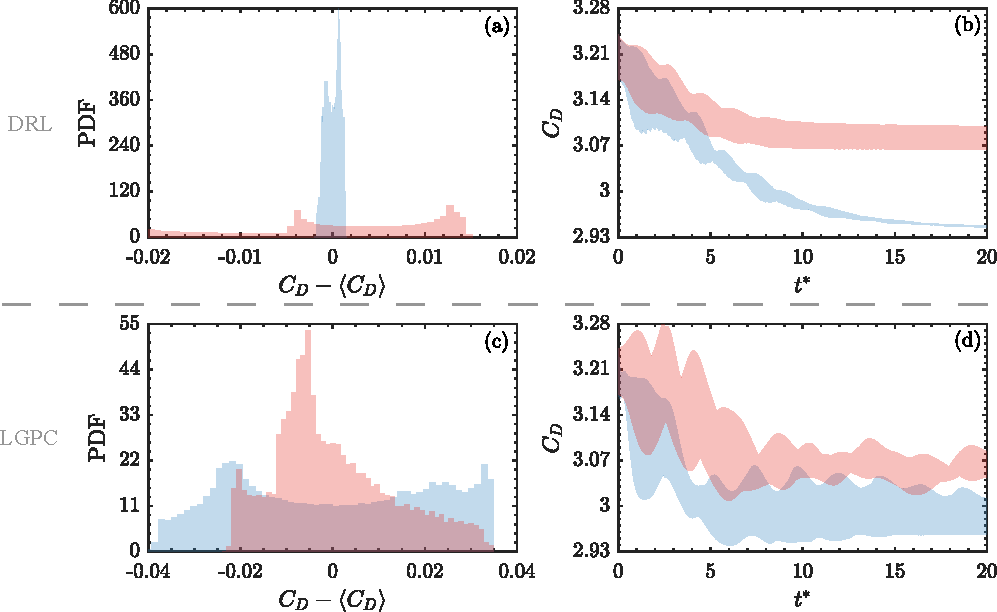
\includegraphics[width=0.99\linewidth]{Figures/4.pdf}
    \caption{Influence of the initial condition on the control performance. Results are shown for DRL (a-b) and LGPC (c-d). The probability density function (a,c) and the $C_D$ envelope (b,d) are computed from the $C_D$ profiles extracted for 55 equispaced initial phases over the whole unperturbed shedding cycle. Distributions are shown for 5 \sy{redRr}{rec} and 11 \sy{blueRr}{rec} probes.}
    \label{fig:Clean_rIC}
\end{figure}

DRL and LGPC are first trained on clean data, i.e. in absence of noise. It is important to remark that the performance of each selected actuation depends on the corresponding flow condition when the actuation is started, i.e. the same control law (or weight distribution for the ANN) determine different performances if run under different initial condition.

\begin{figure}[t]
    \centering
    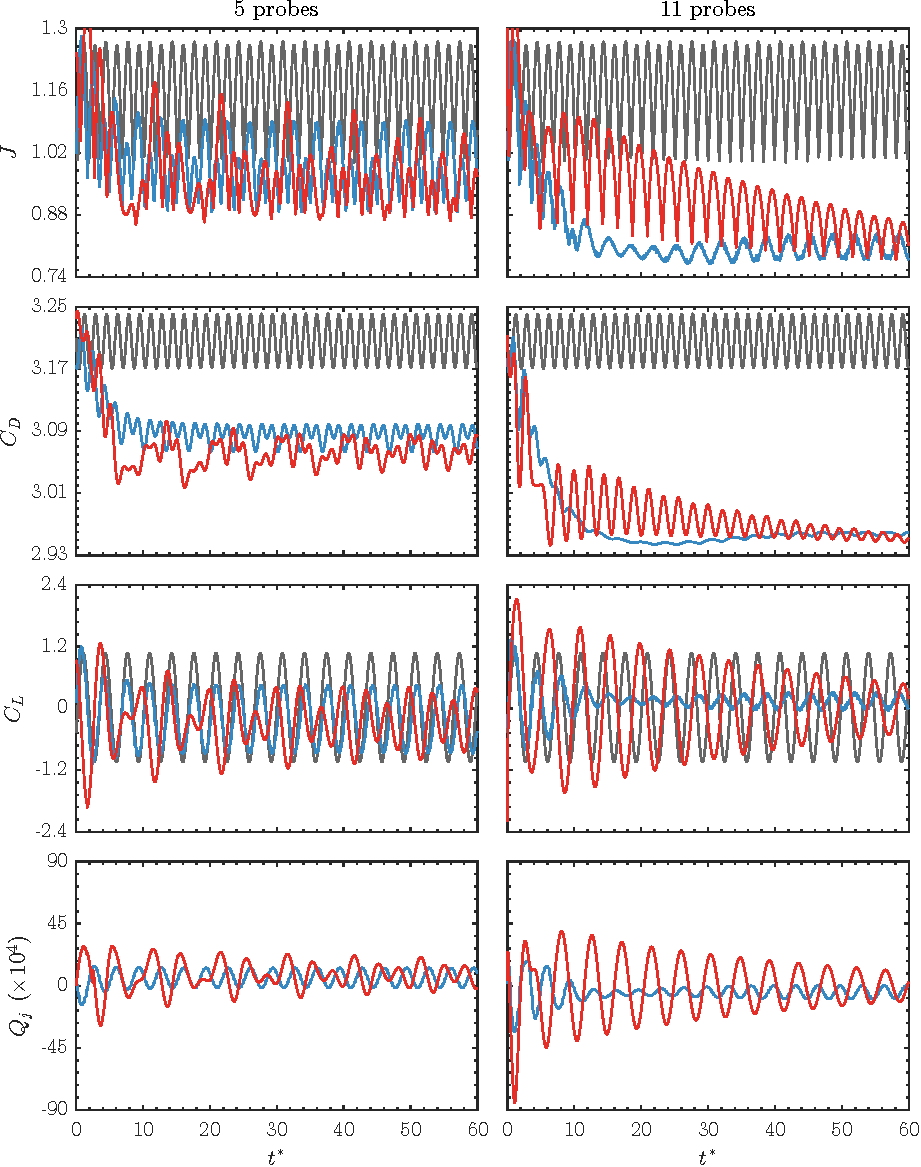
\includegraphics[width=0.9\linewidth]{Figures/5.pdf}
    \caption{Evolution of $J$, $C_D$, $C_L$, and $Q_j$ upon the actuation of DRL \lcap{-}{blueR}, and LGPC \lcap{-}{redR} for 5 and 11 probes. Unforced case \lcap{-}{greyR} shown for reference.}
    \label{fig:Clean_rIC_history}
\end{figure}

The probability distribution function (PDF) of the drag coefficient for the final selected actuation after training is illustrated in Figure \ref{fig:Clean_rIC}(a) for the case of the DRL, and in Figure \ref{fig:Clean_rIC}(c)c for LGPC, both considering 5 and 11 probes. These distributions are obtained analyzing the $C_D$ value obtained running the simulation with 55 equispaced initial phases over the whole unperturbed shedding cycle and averaging the last $650$ simulations steps, corresponding to $3.25t^*$ (being $t^* = t U_\infty/D$ and $U_\infty$ the freestream velocity), i.e. a shedding period of the unforced configuration. This is the same time interval adopted for the computation of the cost function $J$.

The PDF demonstrates that the DRL is less sensitive to the effect of the initial condition if compared to LGPC. This result is not surprising, considering that the agent of the DRL is more complex than the control laws obtained through LGPC (see Table \ref{tab:ControlLawsMLC}), thus it is potentially more flexible to variable initial conditions. While this is a desirable aspect of DRL, on the downside it comes at the expense of a less interpretable control policy. A bit more surprisingly, DRL shows a degradation in performance when passing from $11$ to $151$ probes, which is the case evaluated by \citet{rabault2019JFM}. As an hypothesis, this might be due to the non-sufficiently complex architecture of the ANN since it is common despite the sensing configuration. The input probe number is an order of magnitude larger for 151 probes, thus possibly requiring a more powerful network for the agent and more intense training. Nonetheless, it can be concluded that increasing the number of probes to a reasonable extent seems to reduce the variability of the drag coefficient, thus delivering reliable and robust action against variable initial conditions. This is also observed in Figure \ref{fig:Clean_rIC}b, where the envelope of the drag coefficient history in the set of analyzed initial conditions is presented. The shaded region is centred on the mean drag coefficient at each instant, and the half-width is set to one standard deviation of the drag coefficient. The mean values corresponding to such initial conditions are reported in Table \ref{tab:SummaryResults}.

Observing the results for LGPC, it can be observed that it benefits mainly in terms of average drag coefficient when increasing the probe number (see Figure \ref{fig:Clean_rIC}d), although there is no significant impact on the dispersion of the drag coefficient.

The time history of the cost function $J$, the drag and lift coefficients $C_D,C_L$ and the flow rate of the actuator $Q_j$, are reported in Figure \ref{fig:Clean_rIC_history} for the final selected actuation after training of DRL and LGPC. The initial condition is selected among the $50$ tested cases like the one resulting in a final drag coefficient closest to the mean value. The results are presented for $5$ and $11$ probes, including the case without actuation as a reference. 

In the limit of low probe number ($5$ probes), LGPC is observed to have slightly superior performance than DRL in terms of $C_D$. The average lift coefficient in the final phases of the observation horizon is in both cases weakly negative (i.e. LGPC and DRL converge to an asymmetric flow configuration determined by the control action). This effect is slightly more significant for LGPC, thus showing that the actuation is also aiming to alter the flow symmetry to reduce drag. In terms of the actuation flow rate, DRL converges to a substantially lower standard deviation of the flow rate of a single jet (used here as a parameter, since the net mass flow rate is zero), thus meaning that it requires less power consumption for the actuation. 

The differences are more significant for the case with $11$ probes. The actuation obtained with DRL features a faster convergence to the asymptotic drag and lift coefficient, with minimal fluctuations of the latter. This is achieved with strong action in the initial phase, which rapidly damps to a significantly lower intensity to counteract the triggering of the shedding. The actuation identified by LGCP, on the other hand, needs a significantly longer time to converge. The performances in terms of final drag coefficient are similar to DRL, although the oscillations of the lift coefficient and the flow rate of the actuators are more significant. It is nonetheless remarkable the simplicity of the obtained control law (see Table \ref{tab:ControlLawsMLC}). For the case of 11 probes with a random initial condition, LGPC converges to a law that involves only two probes, both using the crosswise velocity component, located in the middle and on one side of the cylinder (see Figure \ref{fig:NumericalSetup} for probe numbering). Remarkably, LGPC is able to identify the flow symmetry and address time-delayed feedback (for probe 2 the control law also includes a time-delayed signal with a delay of $3/4$ of the period). While the identified control law seems less robust to the effect of the initial conditions, it leads to identifying a subset of probes that is sufficient to obtain effective control.

\subsection{Robustness to measurement noise}
\label{ss:noise}

In this section, the robustness of DRL and LGPC in presence of noise is addressed. Additive noise with Gaussian distribution is included in the sensor data. Three noise levels are investigated, i.e. $1\%,5\%$ and $10\%$ of the freestream velocity.

\begin{figure}[t]
    \centering
    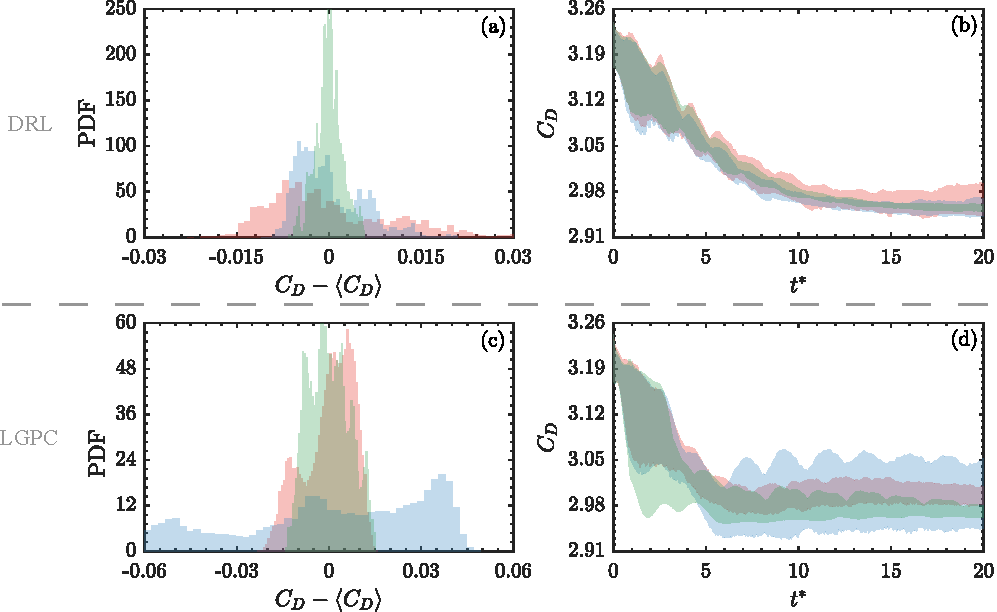
\includegraphics[width=0.99\linewidth]{Figures/6.pdf}
    \caption{Influence of the initial condition on the control performance in the presence of noise. Results are shown for DRL (a-b) and LGPC (c-d). The probability density function (a,c) and the $C_D$ envelope (b,d) are computed from the $C_D$ profiles extracted for 55 equispaced initial phases over the whole unperturbed shedding cycle. Distributions are shown for 1\% \sy{greenRr}{rec}, 5\% \sy{blueRr}{rec}, and 10\% \sy{redRr}{rec} noise level.}
    \label{fig:Noise_rIC_pdf}
\end{figure}


\begin{figure}[t]
    \centering
    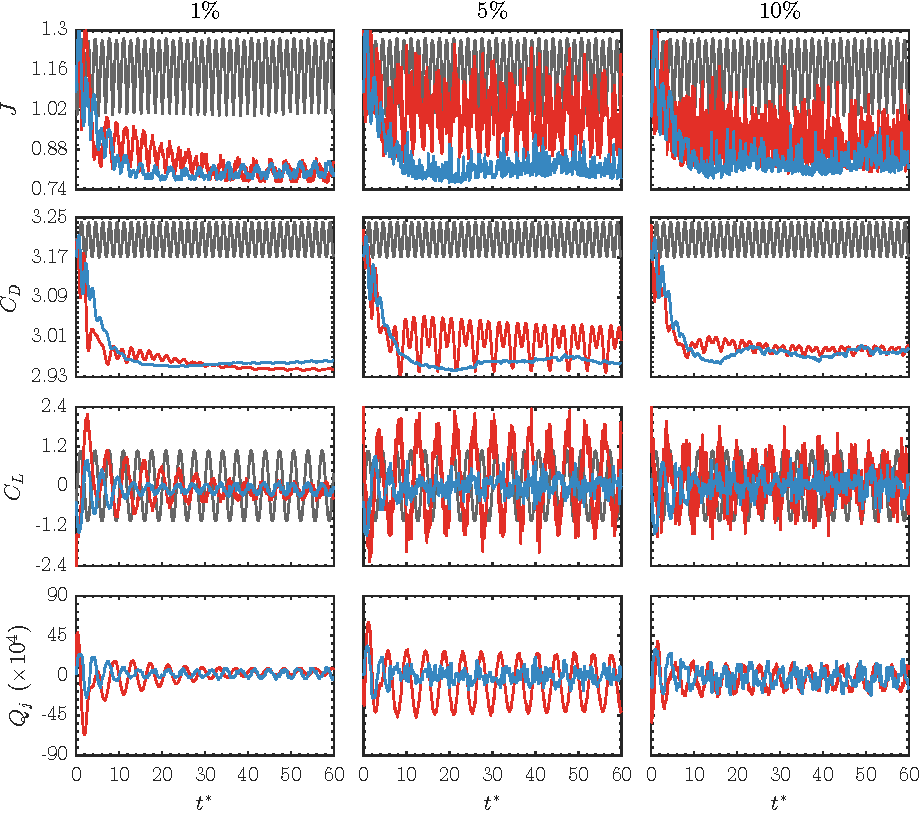
\includegraphics[width=0.95\linewidth]{Figures/7.pdf}
    \caption{Evolution of $J$, $C_D$, $C_L$, and $Q_j$ upon the actuation of the DRL \lcap{-}{blueR}, and LGPC \lcap{-}{redR} controller in the presence of  1\%, 5\% and 10\% noise levels. Unforced case \lcap{-}{greyR} shown for reference.}
    \label{fig:Noise_rIC_history}
\end{figure}

Similarly to the \S \ref{ss:variableIC}, the final actuation policy obtained after training is tested under a range of initial conditions for the case of $11$ probes. The PDF of the drag coefficient, as well as its time evolution and the corresponding dispersion for different initial conditions, are illustrated in Figure \ref{fig:Noise_rIC_pdf}a,b. For the DRL, the scatter around the mean drag coefficient is not significantly affected in the initial steps of the actuation ($t^*<5$), in which the actuation is aiming to displace the flow configuration from one limit cycle to another. For larger times, the dispersion around the mean drag coefficient seems to increase with the noise level, as expected. The final achieved performance shows only a minor degradation for noise levels up to $5\%$, while the penalty becomes more significant at $10\%$ noise level. 
Figure \ref{fig:Noise_rIC_history} reports the evolution with time of the cost function, drag and lift coefficients and actuator flow rate for different noise levels. The initial condition is chosen according to the PDF of the drag coefficient. It is set to be the one yielding the  drag coefficient most similar to the mean. It can be observed that the agent is capable to obtain in all tested cases a drag coefficient with relatively small fluctuations, while the lift coefficient experiences larger variations with the increasing noise level. This is expected since the lift coefficient is directly affected by the asymmetry introduced by the actuation, whose flow rate is directly related by the agent to the signal recorded by the probes. The drag coefficient, on the other hand, is related to the wake configuration and thus the effect is partially damped. Interestingly enough, the results reported in Table \ref{tab:SummaryResults} also show that the average lift coefficient is close to zero, i.e. the noise has the effect of avoiding the agent tricking the policy to achieve drag reduction by introducing asymmetries.

For the case of LGPC, the effect of noise appears more significant, as illustrated in Figure \ref{fig:Noise_rIC_pdf}c,d. According to the results in Table \ref{tab:SummaryResults}, the drag coefficient is quite significantly affected by increasing noise. Interestingly, for the noise level of $1\%$ and $5\%$, the obtained control law is relatively simple and still identifies that 2 probes are sufficient to perform an effective control action. In particular, probe 6 and an off-axis probe (either 2 or 7) are selected in both cases. The history of the cost function, force coefficients and actuator flow rate are also presented in Figure \ref{fig:Noise_rIC_history}. It is indeed confirmed that, for the case of low noise, the optimization successfully reduce the drag coefficient and the oscillations of the lift coefficient, with even more satisfying results than for the case without noise. For larger noise levels, the control law identified by LGPC is not capable of reducing the oscillations of the lift coefficients, thus inevitably affecting also the share of drag coefficient ascribed to vortex shedding.

A direct undesirable consequence of the simplicity of the control law is that, with the increasing noise level, the action is less effective. The different effects of noise between DRL and LGPC can be addressed on one side by the different complexity of the policy, and on the other side by the procedure to determine the action. As described in \S \ref{s:Methodology}, the action selected by the DRL agent is obtained by weighting the current ANN output with the previous step control action, thus introducing a certain soothing effect. It can be speculated that low-pass filtering of the probe signal could improve LGPC performance. Nonetheless, for fairness of comparison, we maintained the same implementation of LGPC presented originally by \citet{li2017GP}, and leave this as an object for future study.

The robustness study against noise for the 5 probes configuration leads to similar conclusions as for the 11 probes case. Hence, for the sake of brevity, it is not included. With a smaller number of probes, a higher noise is observed, as filtering out noise becomes more difficult. The probes in the wake of the cylinder have shown to be the most relevant for feedback because the vortex shedding is more pronounced and the signal-to-noise ratio is better. Intriguingly, LGPC has shown to have lower performance degradation than DRL when using only 5 probes. This is not surprising, since all the control laws extracted with LGPC in the 11 probe case lead to parsimonious use of probes, rarely exceeding 3 or 4 sensors.

%%%%%%%%%%%%%%%%%%%%%%%%%%%%%%%%%%%%%%%%%%%%%%%%%%%%%%%%%%%%%%%%%%%%%%%%%%%%%%%%%%%%
%%%%%%%%%%%%%%%%%%%%%%%%%%%%%%%%% Interpretability %%%%%%%%%%%%%%%%%%%%%%%%%%%%%%%%%
%%%%%%%%%%%%%%%%%%%%%%%%%%%%%%%%%%%%%%%%%%%%%%%%%%%%%%%%%%%%%%%%%%%%%%%%%%%%%%%%%%%%
\begin{figure}[t]
    \centering
    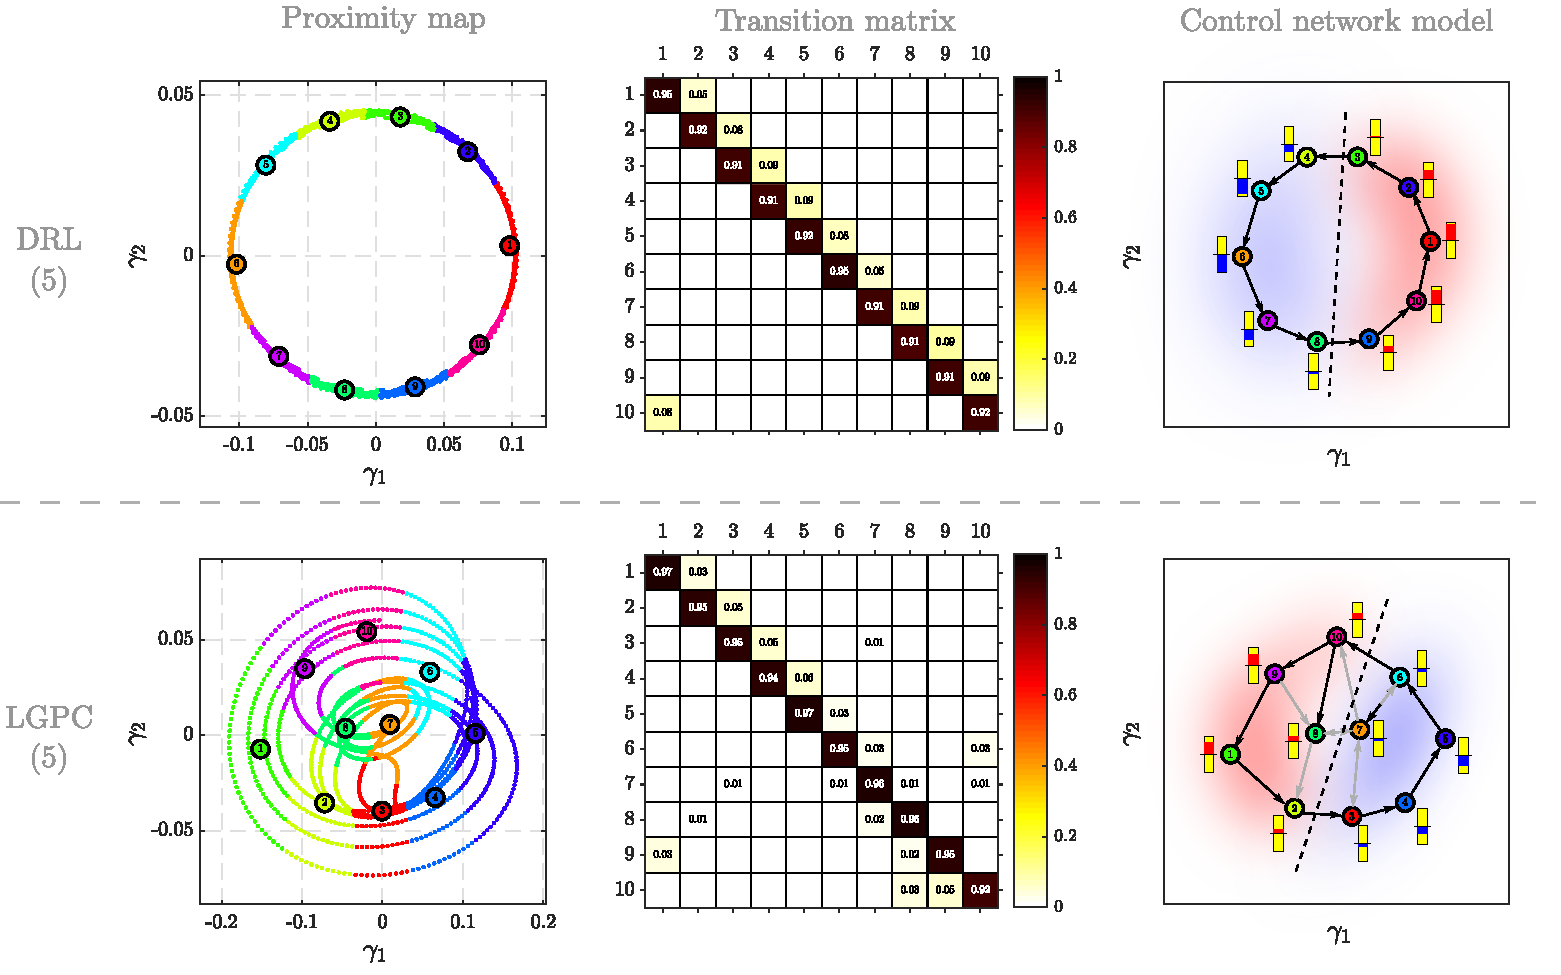
\includegraphics[width=0.95\linewidth]{Figures/8.pdf}
    \caption{Visualization of the laws/policies learned by DRL (top) and LGPC (bottom) for the 5-sensor configuration. (left) The proximity maps of the sensor signals of the controlled regime show each cluster in a different colour with their centroids denoted by numbers (1-10). (centre) The transition matrix is associated with the clustering process. (right) The control network. The yellow boxes set the maximum range of $b$ during the control and the red and blue boxes indicates positive and negative levels (the sign of $b$). The dashed line and red/blue background indicate the assumed separation between the actuation regions.} \label{fig:CL_S5}
\end{figure}
%
\begin{figure}[h!]
    \centering
    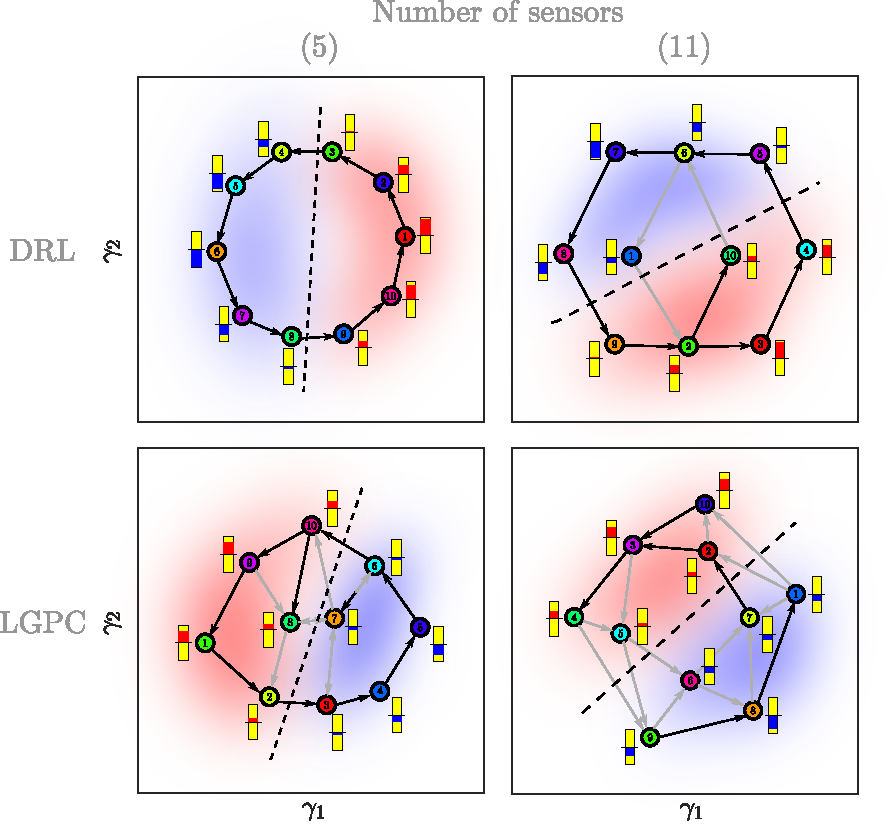
\includegraphics[width=0.7\linewidth]{Figures/9.pdf}
    \caption{Control network for laws/policies learned by DRL (top) and LGPC (bottom) for the 5 (left) and 11 (right) probes. For more details see the caption of Figure~\ref{fig:CL_S5}}
    \label{fig:CL_S}
\end{figure}

\section{Control results and discussion \label{s:interpretability}}
In this section, the controls achieved by DRL and LGPC are analysed with the clustering method described in \S~\ref{Sec:Method_ControlLawVisu}.

\begin{figure}[t]
    \centering
    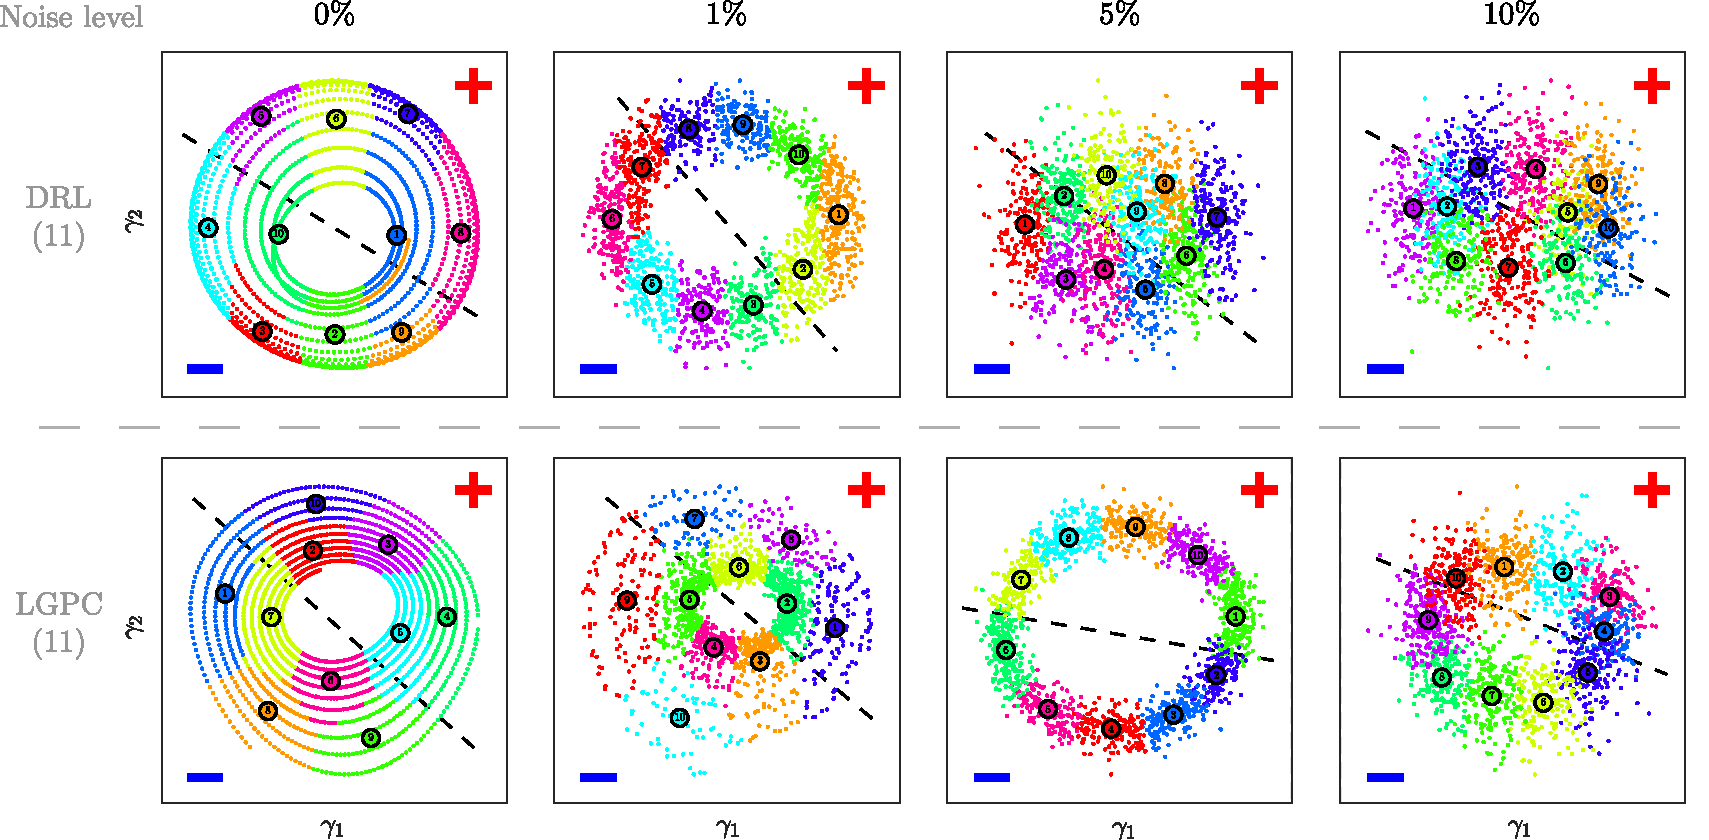
\includegraphics[width=0.99\linewidth]{Figures/10.pdf}
    \caption{Proximity map of the clustered sensors and centroids for the velocity time series extracted from the DRL/LGPC controls with increasing noise. The noise intensity increases from left to right: $0\%$, $1\%$, $5\%$ and $10\%$. The dashed black line divides the reconstructed phase space into two regions: one of positive actuation and one with negative actuation (the sign of $b$) denoted respectively by a red $+$ and a blue $-$. The $\gamma_1$ and $\gamma_2$ axis have been reflected such the red $+$ is located in the top right corner for all cases.}
    \label{fig:CL_Noise}
\end{figure}

For all cases the transient has been excluded by the analysis by removing the first $3000$ time steps, corresponding to $15t^*$. It must be remarked, however, that for the LGPC cases with 0\% and 1\%-level noise, the transient lasts for more than the observed $60$ time units.

Figure~\ref{fig:CL_S5} shows the cluster-based interpretation methodology applied to the laws/policies learned by DRL and LGPC for the 5-sensor cases without noise. The interpretation methodology is applied independently to each case. First, note that the proximity maps of the sensor time series are reminiscent of phase space. Such visualization is not surprising as the controlled flow remains mainly periodic and therefore can be represented in a 2D space. The transition matrices display high probabilities for the self-transitions (diagonal values). This is due to the high sampling rate that excessively populates each centroid. The transition states are then under-represented, hence the low values of the transition probabilities outside the diagonal. Thus, the sensor time series have been subsampled to 1/5th of the data to artificially increase the transition probabilities located outside the diagonal. This operation is done to render the transition matrix easier to read while it does not change either the results or the interpretations. For the DRL control case, note that for each cluster there is only one arrival cluster. This is translated in the control network by a cycle that can be interpreted as a limit cycle in the phase space. For the LGPC case, a limit cycle can also be inferred from the data. However, two centroids close to the centre of the limit cycle (centroids 7 and 8) play a role in short-circuiting the limit cycle. Concerning the control achieved, in both cases, the plane is divided into two regions: one of positive actuation including half the centroids and one of negative actuation including the other half. Furthermore, note that the actuation level increases with the distance to the dividing line. Such organization of the actuation around a limit cycle indicates that the actuation mechanism employed for drag reduction is phasor control, meaning that the control depends on the flow phase.

In addition to this visualization, an analysis combining the two dynamics (not included here for brevity) is performed. For this, the time series have been appended and 20 centroids have been chosen for the description of the flow. The resulting proximity map shows the two limit cycles on the same plane, almost concentric, revealing that the controlled flows are close dynamically. However, the probability transition matrix loses the dynamic relationship between the centroids as some clusters contain states from both learning strategies. 

Figure~\ref{fig:CL_S}, displays the control network for both the number of sensors (5 and 11). Note that the overall shape and relations between the centroids remain the same when going from $5$ sensors to $11$ sensors. Again, the main limit cycle is divided into two regions of positive and negative actuation revealing, again, a phasor control mechanism.

Finally, the impact of noise on the actuation mechanism is investigated. Figure~\ref{fig:CL_Noise} displays time series and the centroids projected in the proximity map for the controlled flows with increasing noise. First, note that going from $0\%$ to $1\%$, the noise disturbs the smooth distribution of data. For DRL, as the noise level increases the clusters starts to overlap so much that for the $10\%$-level noise case, separating visually the clusters becomes impossible on the proximity map. The resulting control network, not plotted because of its complexity, shows that for the post-transient regime the dynamics are mainly driven by the noise. Nonetheless, note that the centroids are distributed around an ellipsoid, indicating a periodicity in the flow. As for the LGPC cases, the proximity maps describe successfully the controlled dynamics. For 0\% and 1\%-noise level, the centroids describe a spiral which is consistent with the long transients (see corresponding lift coefficient $C_L$ in figures~\ref{fig:Noise_rIC_history} and \ref{fig:Noise_rIC_pdf}). For the 5\%-noise level, the persistent high-amplitude oscillations plotted in figure~\ref{fig:Noise_rIC_history} are represented by a clear limit cycle in the proximity map and for the 10\%-noise level, the centroids describe a cycle blurred by the noise which is consistent with the low-amplitude oscillations of the lift coefficient in the post-transient regime (figure~\ref{fig:Noise_rIC_history}). In summary, in all the cases, the flow includes a periodic behaviour. Regarding the actuation command, all the proximity maps can be separated into two regions, one of positive actuation and negative actuation, indicating that both DRL and LGPC managed to learn a phasor control regardless of the noise level.

\section{Conclusions}\label{s:Conclusions}

Two machine-learning-based strategies which minimize the drag of a cylinder exhibiting vortex shedding wake are evaluated. The performance of Deep Reinforcement Learning and Linear Genetic Programming Control in identifying effective control policies has been assessed in the realistic conditions of a limited number of sensors and noise contamination of the sensed data. The training is performed using random initial conditions, in the attempt to reproduce an experimental scenario in which it is not feasible to control the full flow state when the actuation is started.

It is observed that, in absence of noise, the average performance achieved by DRL and LGPC is similar in terms of average lift and drag coefficient, although with a significant advantage of the DRL in terms of the standard deviation of the mass flow rate of the actuation. It must be remarked, however, that the amount of power needed to control has not been included in the loss function. Furthermore, the policy obtained by DRL appears to be more robust in terms of dependency on the initial condition. On the other hand, LGPC achieves significantly more compact and interpretable control laws, which also identify only subsets of the probes as being relevant to define control actions. In particular, for the cases with 11 probes and low to moderate noise levels, LGPC identifies that only 2 probes are sufficient to define a sufficiently robust control law. The potential reduction in sensorization complexity is a very desirable feature for experimental application. 

Regarding the effect of noise, DRL shows superior performances in terms of robustness to noise of the sensors up to relatively high noise levels (10\%). LGPC, on the other hand, is able to identify control laws that are effective in reducing the average drag coefficient, although maintaining a larger level of fluctuations around the mean lift and drag coefficient if compared to DRL, and in general larger standard deviation of the actuator mass flow rate. This superior robustness of the DRL can certainly be ascribed to the higher complexity of the adopted agent if compared to the control policies identified by LGPC. Also in presence of noise, LGPC converges to compact control laws and automatically identifies only a few significant probes for the control, almost independently of the noise level within the tested range.

Finally, an analysis using clustering of the sensor data using MDS has been carried out to interpret the control laws obtained by DRL and LGPC. In absence of noise, it is rather evident the convergence to a limit cycle in both cases and a clear relation between the phase of the shedding and the control actuation. This is an indicator that both solutions converge to phasor control, which was an expected result for this simple flow configuration. 

Although the number of sensors might seem high for a real application, it is remarkable that this study has already considerably reduced the number of probes compared to other recent contributions~\citep{Ren2021pof,rabault2019DRL,rabault2019JFM}. Having a smaller set of probes is viable but not recommended for a proof of concept as the one presented herein, since the information provided to the controller would be very limited and hence the solution would probably be suboptimal. The chosen sets of sensors allow testing the performance of both algorithms and also evaluate their relevance for the final controller. Consequently, one of the main conclusions of the study is the capability of LGPC of identifying a subset of probes as the most relevant, which suggests the possibility of further reduction. This is a milestone for future implementations in a real-world application or experiment.

Any comparison contains subjective biases associated with the computational load, the number of parameters, the complexity of the control problem, and even the experience of authors with various approaches. Also, each approach could have been improved. e.g., DRL has many architectures with different performances and LGPC consistently profits from subplex iterations\citep{cornejo2021gMLC}. Even, the very formulation of the control ansatz will affect the performance. Yet, our study points already to desirable features of two different machine learning approaches. Future machine learning control can be expected to integrate the fast adaptive learning of DRL, the analytical laws and interpretability of LGPC, the fast optimization of cluster-based control for smooth control laws\citep{Nair2019jfm} and the mathematically rigorous framework of Bayesian optimization\citep{Blanchard2022ams}, to name only a few aspects.

\section*{Acknowledgments}
Work produced with the support of a 2020 Leonardo Grant for Researchers and Cultural Creators, BBVA Foundation, grant n. IN[20]\_ING\_ING\_0163. The Foundation takes no responsibility for the opinions, statements and contents of this project, which are entirely the responsibility of its authors.

Funding of the National Natural Science Foundation China (NSFC) under grants 12172109 and 12172111 and a Natural Science \& Engineering grant of the Guangdong province, China, is gratefully acknowledged. 

\section*{Data Availability Statement}
The data that support the findings of this study are available from the corresponding author upon reasonable request.
%%%%%%%%%%%%%%%%%%%%%%%%%%%%%%%%%%%%%%%%%%%%%%%%%%%%%%%%%%%%%%%%%%%%%%
%%%%%%%%%%%%%%%%%%%%%%%%%%% Appendix %%%%%%%%%%%%%%%%%%%%%%%%%%%%%%%%%
%%%%%%%%%%%%%%%%%%%%%%%%%%%%%%%%%%%%%%%%%%%%%%%%%%%%%%%%%%%%%%%%%%%%%%
\appendix
\section{Flow control performance training at fixed Initial Condition}
\label{ss:fixedIC}

\begin{figure}[tb]
    \centering
    \includegraphics[width=0.99\linewidth]{Figures/11_v2.pdf}
    \caption{Evolution of $J$, $C_D$, $C_L$, and $Q_j$ for the unforced case \lcap{-}{greyR}, RL \lcap{-}{blueR}, and LGPC \lcap{-}{redR} at fixed initial condition during the training process. Results are shown 11 probes.}
    \label{fig:Clean_fIC}
\end{figure}

The case with training starting from a fixed initial condition is analyzed here. Although this condition is difficult (if not impossible) to achieve in experiments, it can be approximated reasonably well in the case of shedding-dominated flows at a low-to-moderate Reynolds number. The evolution of the cost function, the force coefficients and the actuator flow rate are reported in Figure \ref{fig:Clean_fIC} for the case of the final resulting actuation after the training. For brevity, only the case with 11 probes is analyzed.

\begin{figure}[tb]
    \centering
    \includegraphics[width=0.95\linewidth]{Figures/12.pdf}
    \caption{Key performance indicators, cost function $\langle J \rangle$ (left) and drag reduction $-\Delta \langle C_D \rangle = \frac{\langle C_{D_0} \rangle - \langle C_{D_0} \rangle}{\langle C_{D} \rangle}$ (right), for random \sy{blueR}{rec} and fixed \sy{redR}{rec} initial condition.}
    \label{fig:barplot}
\end{figure}

Since in this case the initial condition for DRL and LGPC is the same, it is interesting to compare the different strategies adopted by the two control laws to bring the system to a different limit cycle than the original unperturbed system. In the first shedding cycle, the control law identified by LGPC acts with a strong blowing on the top actuator, thus determining a significant asymmetric and a net negative lift coefficient. On the other hand, DRL acts with a quasi-periodic change in phase in opposition to the original shedding cycle.

While the performance in terms of drag coefficient is similar for DRL and LGPC, more significant differences arise in the lift coefficient. The control law identified by DRL reduces more significantly the oscillation of the $C_L$, thus also requiring a smaller actuator flow rate for the control action. The bar plot of the cost function and of the drag coefficient reduction in figure~\ref{fig:barplot} further support this assertion. For both LPGC and DRL, a reduction in performances when passing from random to fixed initial condition is observed. This is a first glance surprising; it is hypothesized that having a random initial condition aids the exploration in both algorithms, allowing the discovery of more robust control strategies.

Surprisingly, even if using the same set of probes, LGPC exhibits a much more complex control law if compared to the random initial condition case, and fails to identify a compact law,

\begin{equation*}
    \begin{split}
        Q_{jet} = 10^{-2} \times \left[
        \left(\left(u_7\left(t-\frac{T}{2}\right) \cdot \left(v_6+u_6\left(t-\frac{3T}{4}\right)\right)\right)+ \right.\right. \\
        \left.\left. \left(0.1551-\left(u_8\left(t-\frac{3T}{4}\right) \cdot \left(v_0\left(t-\frac{T}{4}\right) \right.\right.\right.\right.\right.+ \\
        \left.\left.\left.\left.\left. \left(v_9\left(t-\frac{T}{2}\right)-u_0\left(t-\frac{T}{4}\right)\right)\right)\right)\right)\right)*cos\left(u_7\left(t-\frac{T}{2}\right)\right)\right]
    \end{split}
\end{equation*}\\

This might be ascribed to a tendency of the algorithm to overfit the control law to the prescribed initial condition.\\
\vspace{1cm}
%%%%%%%%%%%%%%%%%%%%%%%%%%%%%%%%%%%%%%%%%%%%%%%%%%%%%%%%%%%%%%%%%%%%%%



%------------------------------------------------------------------------------
% Bibliography
%------------------------------------------------------------------------------
%
%\clearpage
\bibliographystyle{jfm}
\bibliography{paper3/bib3}
%
\IfFileExists{paper3/bib3.bbl}{\input{paper3/bib3.bbl}}{}


%===============================================================================
%                            END PAPER
%===============================================================================
\end{paper}

%-------------------------------------------------------------------------------
% Paper 5: LGAC for HTE
%------------------------------------------------------------------------------
% Define title, author(s), affiliation and publishing status
%
\papertitle[Genetically-inspired convective heat transfer enhancement in a TBL] % Short title used in healines (optional)
{%
Genetically-inspired convective heat transfer enhancement in a turbulent boundary layer% THE COMMENT SYMBOL AT THE END OF THIS LINE IS NEEDED
}%
%
\papertoctitle{Genetically-inspired convective heat transfer enhancement in a turbulent boundary layer} % Title for toc
%
\paperauthor[R. Castellanos \etal] % Short authors used in headlines and List Of Papers
{%
  Rodrigo Castellanos$^{1,2}$, Andrea Ianiro$^1$ \& Stefano Discetti$^{1}$%
}%
%
\listpaperauthor{Castellanos, R., Ianiro, I. \& Discetti, S.}% (optional) Short authors used in List Of Papers
%
\paperaffiliation
{%
  $^1$ Aerospace Engineering Research Group, Universidad Carlos III de Madrid, Legan\'{e}s 28911, Spain\\%
  $^2$ Theoretical and Computational Aerodynamics Branch, Flight Physics Department, Spanish National Institute for Aerospace Technology (INTA), Torrej\'on de Ardoz 28850, Spain.
}%
%
\paperjournal[Appl. Therm. Eng.] % Short publish info used in List Of Papers
{%
	Applied Thermal Engineering%
}%
%
\papervolume{Submitted}%
%
%\papernumber{--}
%
%\paperpages{--}%
%
\paperyear{2022}%
%
\papersummary%
{% Insert summary of the paper here (used in introduction)
The convective heat transfer enhancement in a turbulent boundary layer (TBL) on a flat plate is optimised using an artificial intelligence control based on linear genetic algorithms control (LGAC). The control consists of the pulsation of a spanwise array of six slot jets in cross flow. The open-loop periodic forcing is driven by the carrier frequency, the duty cycle and the phase between actuators as control parameters. The control laws are optimised with respect to the unperturbed TBL and the steady-jet actuation case, leading to a multi-objective optimisation problem. The performance of the controller is characterised based on infrared thermography and particle image velocimetry measurements. The action of the jets considerably alters the flow topology compared to the steady-jet actuation. The optimal controller yields an asymmetric flow field. The LGAC algorithm converges to a characteristic frequency of the system for all the actuators, fixing the duty cycle. It is noted that such frequency is strikingly equal to the inverse of the characteristic travel time of large-scale turbulent structures convected within the buffer layer. The phase difference between multiple jet actuations has shown to be very relevant and the main driver of the flow asymmetry. The results point to the exceptional potential of machine learning control in unravelling unexplored controllers within the actuation space. Our study demonstrates the viability of employing sophisticated measurement techniques together with advanced algorithms in an experimental investigation.
}
%
\graphicspath{{paper5/}}%
%
%
%===============================================================================
%                            BEGIN PAPER
%===============================================================================
%
\begin{paper}

\makepapertitle

%------------------------------------------------------------------------------
% Abstract
%------------------------------------------------------------------------------
%
\begin{paperabstract}
The convective heat transfer enhancement in a turbulent boundary layer (TBL) on a flat plate is optimised using an artificial intelligence control based on linear genetic algorithms control (LGAC). The control consists of the pulsation of a spanwise array of six slot jets in cross flow. The open-loop periodic forcing is driven by the carrier frequency, the duty cycle and the phase between actuators as control parameters. The control laws are optimised with respect to the unperturbed TBL and the steady-jet actuation case, leading to a multi-objective optimisation problem. The performance of the controller is characterised based on infrared thermography and particle image velocimetry measurements. The action of the jets considerably alters the flow topology compared to the steady-jet actuation. The optimal controller yields an asymmetric flow field. The LGAC algorithm converges to a characteristic frequency of the system for all the actuators, fixing the duty cycle. It is noted that such frequency is strikingly equal to the inverse of the characteristic travel time of large-scale turbulent structures convected within the buffer layer. The phase difference between multiple jet actuations has shown to be very relevant and the main driver of the flow asymmetry. The results point to the exceptional potential of machine learning control in unravelling unexplored controllers within the actuation space. Our study demonstrates the viability of employing sophisticated measurement techniques together with advanced algorithms in an experimental investigation.

        \keywords{Machine learning, Genetic algorithms, Flow control, Pulsed jet in crossflow, Turbulent Boundary layers, Convective heat transfer enhancement}
\end{paperabstract}


%------------------------------------------------------------------------------
% Article
%------------------------------------------------------------------------------
%
%%%%%%%%%%%%%%%%%%%%%%%%%%%%%%%%%%%%%%%%%%%%%%%
\definecolor{blue}{rgb}{0,0,1}
\definecolor{red}{rgb}{1,0,0}
\definecolor{black}{rgb}{0,0,0}
\definecolor{grey}{rgb}{0.775,0.775,0.775}
\definecolor{white}{rgb}{1,1,1}

\definecolor{BlueTBL1}{rgb}{0.41961,0.682353,0.839216}
\definecolor{BlueTBL2}{rgb}{0.12941,0.443137,0.709804}
\definecolor{green_laser}{RGB}{0,208,0}
\definecolor{green_lgac}{rgb}{0.1068,0.5190,0.2488}
\definecolor{red_lgac}{rgb}{0.7630,0.0863,0.1068}
\definecolor{blue_lgac}{rgb}{0.1076,0.4153,0.6880}
\definecolor{red_pod_1}{rgb}{0.9467,0.2682,0.1961}
\definecolor{red_pod_2}{rgb}{0.7365,0.0800,0.1012}
\definecolor{red_pod_3}{rgb}{0.4039,0,0.0510}
%%%%%%%%%%%%%%%%%%%%%%%%%%%%%%%%%%%%%%%%%%%%%%

%%%%%%%%%%%%%%%%%%%%%%%%%%%%%%%%%%%%%%%%%%%%%%%%%%%%%%%%%%%%%%%%%%%%%%%
%%%%%%%%%%%%%%%%%%%%%%%%%%%%%%% INTRODUCTION %%%%%%%%%%%%%%%%%%%%%%%%%%%
%%%%%%%%%%%%%%%%%%%%%%%%%%%%%%%%%%%%%%%%%%%%%%%%%%%%%%%%%%%%%%%%%%%%%%%%
\section{Introduction}\label{s:intro}
% P1: Motivation, Artificial Intelligence controller:
%Artificial intelligence, supported by the technological and computational development of the last decade, is here to stay, being one of the most promising research areas in several scientific fields. 
The control of turbulent flows based on artificial intelligence has gained interest due to its versatility and superlative capabilities to deal with the complexity imposed by the non-linearity, time-dependence, and high dimensionality inherent to the Navier-Stokes equations \citep{BruntonNoackKoumoutsakos2020}. In this work, we enhance the convective heat transfer in a turbulent boundary layer (TBL) using a model-free self-learning control method. 

% P1 (bis): Motivation, heat transfer
%Applications such as boundary layer separation control, skin friction reduction or convective heat transfer enhancement motivate the development of methods for turbulent flow control. The majority of available studies focus on the reduction of momentum fluxes in turbulent flows, targeting skin-friction drag; however, convective heat transfer enhancement still raises several challenges, building a technological barrier in fields such as high-power electronics or turbomachinery \citep[see e.g.][]{moore2014emerging,han2012gas}. 

% P2: Passive versus Active:Introduction to JICF
Significant convective heat transfer enhancement in turbulent boundary layer flows has been achieved with passive devices, such as obstacles \citep{mallor2018cubes} or riblets \citep{mallor2019modal} and vortex generators \citep{Ke2019VG}, and active actuators adjust like continuous \citep{puzu2019jet}, synthetic \citep{Giachetti2018synjet}, and pulsed \citep{Castellanos2022slotjet} jets in crossflow, plasma actuators \citep{roy2008plasma}, or electromagnetic forcing \citep{Kenjere2008EMheat}, among others. In this study, the actuator consists of a spanwise array of pulsed slot jets in cross flow (JICF).  The flow physics and the induced structures by JICF is well described in the literature \citep[e.g.][]{cortelezzi2001formation, Getsinger2014}. Jet pulsation can be exploited to optimise a certain flow feature \citep{eroglu2001structure, MCLOSKEY2002, shapiro2006optimization}. For instance, \citet{johari1999penetration} studied the mixing properties of fully-modulated JICF, finding that the frequency and duty cycle are the main control parameters influencing the mixing properties. 

Most of the studies employing JIFC for flow control exploit the formation of a counter-rotating vortex pair for mixing enhancement. Conventionally, the generation of embedded streamwise vortices in the TBL is also considered the main heat transfer enhancement mechanism \citep{jacobi1995}. The numerical study by \citet{Zhang1993heatJICF} concludes that the heat transfer increases due to the entrained fluid towards the wall provided by the induced counter-rotating vortex pair. Likewise, the recent effort by \citet{puzu2019jet} investigates the influence of the jet-induced counter-rotating vortices in the enhancement of heat transfer. The interested reader is referred to the extensive review article by \citet{karagozian2010transverse} covering the jet in crossflow and the control based on it. 

% P3: introduction into control
Effective turbulence control is a challenging task that mainly depends on the phenomena to be controlled and the available information from the system. The flow control problem is commonly posed as an optimisation problem in which a control function is optimised. Active control based on periodic forcing, for instance, may be parameterised by the most relevant control parameters such as the pulsation frequency, the duty cycle or the phase shift between actuators. Some examples are the skin-friction reduction in a TBL by periodic blowing and suction \citep{cheng2021skin}, the periodic pulsation of a jet in cross-flow to enhance heat transfer in a TBL \citep{Castellanos2022slotjet} or mixing in a jet stream \citep{Fan2017jetcontrol}. The performance of the periodic control scales with the size of the feasible solution space; however, the optimisation process becomes more time-consuming. The irruption of artificial intelligence algorithms opens new knowledge gaps in which the usage of more sophisticated optimisation methodologies can lead to outstanding performance enhancements \citep{Noack2019control}. There is a vast collection of mathematical tools for an effective design of the control law, distinguishing between model-based and model-free control depending on whether a model to describe the dynamics is available.

% P4: classical control, model-based
Model-based control stands out when dealing with simplified flow-control problems based on first- or second-order dynamics \citep{Rowley2006control}. Model-based control strategies enable a profound understanding of the dynamics of the actuated system based on the pre-established model. This approach has hitherto struggled in controlling turbulent flows due to the chaotic dynamics of turbulence with countless frequency-crosstalk mechanisms \citep{BruntonNoack2015review}. A few exceptions succeeded in controlling elementary turbulent flows. The linear dynamics can be numerically determined by discretising the Navier-Stokes (N–S) equations  \citep{Kim2007linearcontrol,Sipp2010linearcontrol}. %Also by the projection into a reduced-order subspace composed of several dominant non-normal global stability eigenmodes \citep{akervik2007galerkin}. 
The creation of transfer functions based on the parabolised stability equations allows for the real-time estimation of the wavepacket evolution \citep{sasaki2017wavepackets}. 
%In experiments, from signal and PIV measurements, linear stochastic estimation \citep{Tinney2006LSE} can be used to resolve the flow physics. 
Some other examples related to flow control of first- and second-order dynamics include the near-wall opposition control \citep{Choi1994,Fukagata2003oppcontrol},  two-frequency crosstalk \citep{Glezer2005control,luchtenburg2009galerkin}, oscillations stabilisation via phasor control \citep{pastoor2008control}, and quasi-steady response to quasi-steady actuation \citep{Pfeiffer2018robustcontrol}.

% P5: model-free
The intrinsic challenges posed by turbulence control motivate model-free approaches. Nevertheless, the non-convexity of the feasible solution space for the actuation design represents a challenge. In experimental applications, most of the literature studies simplify the optimisation problem to a few actuation parameters with adaptive variations either based on temporal evolution or sensor signal. Common model-free strategies for turbulence control are the evolutionary algorithms \citep{Koumoutsakos2001evolcontrol} and genetic algorithms \citep{Benard2016ga}. Other examples include the extremum and slope-seeking control method \citep{Krstic2000extremumseek, Becker2007extseek, Gelbert2012extseek} and physics-based methods \citep{pastoor2008control,Zhang2004control}. 

%P6: recent development of model-free
Model-free approaches have been increasingly applied in the last decade, thanks to the popularisation and advances in machine learning techniques. An early precursor is the work by \citet{Lee1997NN} pioneering neural network control for skin-friction drag reduction. Reinforcement Learning (RL) has recently become one of the most prominent model-free control techniques from the machine learning literature \citep{rabault2019JFM,Beintema2020,li2021ReLe,paris2021}. On the other hand, evolutionary algorithms \citep{Dracopoulos1997geneticalg}, rediscovered as machine learning control (MLC), turn up as a promising alternative in flow control applications \citep{duriez2017book,li2017GP}. A comparative assessment of the two methods has been recently published by \citet{Castellanos2022LGPCvsRL}, testing their performance when only a reduced number of (noisy) sensors is available. 

% P7: decision to use MLC based on LGAC and examples
In the current work, we maximise the convective heat transfer enhancement in a turbulent boundary layer. This is a complicated flow-control problem that comprises a wide range of spatial and temporal scales with mutual nonlinear interaction. Model-based control presents strong limitations in presence of highly chaotic flows. The authors are unaware of any promising model-based control study applied to turbulent flows targeted to heat-transfer enhancement. Therefore, we employ MLC based on linear genetic algorithms control (LGAC) for the control logic. Evolutionary algorithms are rather unexplored in the field of heat transfer. The extensive review by \citet{Gosselin2009GareviewHT} describes most of the applications in this field. Most recently, the work by \citet{Tian2020GAheatexchanger} used a genetic algorithm (GA) to increase the efficiency of a spiral double-pipe heat exchanger, and \citet{Moon2021GA-HE} optimised the design of an ultra-compact heat exchanger with a GA. Conversely, MLC has been used in numerous experiments as summarized in the review by \citet{Noack2019control}. %Recently, MLC based on LGAC was used to reduce the skin-friction drag in a TBL by optimising the phase delay among six streamwise-aligned slot jets \citet{Yu2021GA_drag_slot_jets}, finding a non-uniform forcing strategy with 60\% drag reduction. \citet{minelli2020lgac}relied on multi-frequency forcing to control the wake of a bluff body. LGAC finds the set of control parameters that cancel most of the shedding motion after the body, reducing up to 20\% the drag. Similarly, MLC based on genetic programming (GP) has been applied to numerous flow control problems such as jet mixing optimization \citep{zhou2020artificial}, drag reduction past bluff bodies \citep{li2017GP}, shear flow separation control \citep{gautier2015MLC}, reduction of vortex-induced vibrations of a cylinder \citep{Ren2019pof}, and wake stabilization of complex shedding flows \citep{raibaudo2019pof} among others. Recently, an enhanced version of MLC combining linear genetic programming control and classical gradient-descent algorithms was used to stabilise the flow past three rotating cylinders.

% P7: final paragraph
This study focuses on the enhancement of convective heat transfer in a TBL by employing a spanwise array of six slot jets in cross flow. To the author's best knowledge there is no available investigation in the literature similar to that presented herein. We intend to exploit linear genetic algorithms to explore a wide range of actuation parameters. The present manuscript is structured as follows. Section \ref{s:Methodology} defines the experimental apparatus, the measurement techniques and the actuation system, followed by the characterisation of the reference flow conditions in Section~\ref{s:Characterisation}. The optimisation problem is formulated in Section~\ref{s:MLC} together with a description of MLC. Section~\ref{s:Results} collects the results focusing on the evolution of the training process while the discussion of the optimised control law and its effect on the flow gathers in Section~\ref{s:discussion}. Ultimately, the conclusions of the study are drawn in Section \ref{s:Conclusions}.

%%%%%%%%%%%%%%%%%%%%%%%%%%%%%%%%%%%%%%%%%%%%%%%%%%%%%%%%%%%%%%%%%%%%%
%%%%%%%%%%%%%%%%%%%%%%%%%%% METHODOLOGY %%%%%%%%%%%%%%%%%%%%%%%%%%%%%
%%%%%%%%%%%%%%%%%%%%%%%%%%%%%%%%%%%%%%%%%%%%%%%%%%%%%%%%%%%%%%%%%%%%%
\section{Experimental setup and Methodology \label{s:Methodology}}

This section addresses the experimental setup and measurement techniques employed in the study. The actuation system is outlined and the setup for flow field and heat transfer measurement is presented. 

\subsection{Wind tunnel setup and flow conditions \label{ss:WTandBLcond}}%
%
The experimental campaign was held in the G\"ottingen-type wind tunnel at Universidad Carlos III de Madrid. The test chamber expands $1.5\mathrm{m}$ of length with a $0.4 \times 0.4\mathrm{m}^2$ cross-section. The freestream velocity is set for all the test cases at $U_\infty = 12.1\mathrm{m/s}$. The streamwise turbulence intensity is below 1\%.  

The base flow consists of a turbulent boundary layer that develops on a smooth poly-methyl methacrylate flat plate of $1.5\mathrm{m}$ length and $20\mathrm{mm}$ thickness, spanning the entire width of the test section (see figure~\ref{fig:SetUp}(a-b)). The flat plate is designed to host different ad-hoc modules (grey-shaded area in figure~\ref{fig:SetUp}(a)). For this study, the plate is equipped with a 3D-printed flush-mounted module containing a spanwise array of $6$ streamwise-aligned slots and a wall heat flux sensor.

%----------------------------------------------------------
\begin{figure}[t]
    \centering
    \includegraphics[width = 0.99\linewidth]{figures/F1.pdf}
    \caption{Schematic representation of the experimental setup in the wind tunnel: top (a), side (b) and back (c) views. The red dashed area \lcap{--}{red} indicates the IR-thermography measurement domain downstream of the actuator and the green plane \lcap{-}{green_laser} depicts the PIV illumination plane at $y^+=350$ from the wall. (d) The pneumatic system for the jet secondary flow injection.} \label{fig:SetUp}
\end{figure}
%----------------------------------------------------------

%The pressure distribution on the flat plate is characterised to ensure the Zero pressure gradient condition (ZPG).
The leading edge has a wedge shape followed by a tripping device to trigger turbulence transition of the boundary layer. A $210\mathrm{mm}$ long adjustable trailing-edge flap, deflected by approximately $20^\circ$, is used to avoid flow separation at the leading edge. A combination of a $2.5\mathrm{mm}$ height zig-zag turbulators to promote an abrupt transition in combination with a $10\mathrm{mm}$ wide DYMO\textsuperscript{\textregistered} tape (with the embossed letter ‘V’ pointing in the flow direction) to diffuse the vortices shed from the upstream turbulator is used as shown in figure~\ref{fig:SetUp}(a). 

%As further detailed in \S\ref{s:Characterisation}, the TBL is not reminiscent of tripping effects within the measurement region \citep{sanmiguel2017diagnostic}.

A reference system with its origin on the mid-plane of the leading edge of the flat plate is considered. For clarity, the streamwise coordinate $\hat{x}$ (see figure~\ref{fig:SetUp}(a)) will be used throughout the manuscript, defined as $\hat{x} = x - x_{s}$, being $x_{s}$ the upstream edge of the heat-flux sensor (see \S\ref{ss:IR}). Additionally, the following conventions and notations are applied. The velocity components along the streamwise $(x)$, wall-normal $(y)$ and spanwise $(z)$ directions are represented by $U$, $V$ and $W$, respectively. Over-lined symbols refer to ensemble-averaged quantities (e.g. $\overline{U}$) whereas lower-case symbols refer to the fluctuating components (e.g. $u$) according to the classical Reynolds decomposition. Wall-scaled variables are defined in terms of the local friction velocity, $u_\tau$, and kinematic viscosity, $\nu$, and are denoted by a superscript ‘+’. Other quantities used as references throughout the paper are the free-stream velocity, $U_\infty$, and the boundary-layer thickness $\delta$. 

%----------------------------------------------------------------------------
\subsection{Actuation system \label{ss:actuator}}
%----------------------------------------------------------------------------

The actuation system consists of an array of $6$ streamwise-aligned slot jets. The actuators are placed sufficiently far downstream of the leading edge to ensure no reminiscence from the tripping devices ($x = 0.81\mathrm{m}$). The slot jets feature a rectangular cross-section of $25 \mathrm{mm}$ in length and $1 \mathrm{mm}$ in width. The slots are aligned in the streamwise direction with a centre-to-centre spacing between adjacent slots of $7.5 \mathrm{mm}$. A diffuser is designed to ensure a smooth transition from the circular pneumatic line to the rectangular nozzle exit section. The diffuser length of $70 \mathrm{mm}$ is divided in an inlet for a rounded connection of inner diameter $4 \mathrm{mm}$, and an expansion region of $50 \mathrm{mm}$ length with $15^\circ$ opening angle. The enlargement section is equipped with vanes to improve the flow uniformity across the slot width and reduce the pressure losses within the diffuser. The design has been carried out with the support of RANS numerical simulations.  

The pneumatic system is shared among the actuators, as sketched in figure~\ref{fig:SetUp}(d). Compressed air is filtered and regulated to a constant absolute pressure of $P_{jet} = 4.0 (\pm0.005)\mathrm{bar}$ by means of a pressure-relief valve. An Alicat Scientific\texttrademark~\textit{M-100SLPM} flow regulator controls the pressure-relief valve and monitors the flow properties such as absolute pressure, mass and volumetric flow rate, and temperature. Each jet is independently pulsed by a high-speed solenoid valve SMC\textsuperscript{\textregistered}~\textit{SX-11DJ}, with a frequency up to $350~\mathrm{Hz}$. The solenoid valve is triggered by a $24V$ periodic square signal with a characteristic carrier frequency $f$ and duty cycle $DC$. In this study, $DC$ is defined as the ratio between the pulse width $\tau$ and the period $T$, i.e. $DC=\tau/T$.
The square-wave signal driving the actuation is transferred to the valve via a ST\texttrademark~\textit{STM32 Nucleo} board with an independent timer for each valve. 

The instantaneous jet exit velocity at the centre of each slot is confirmed to be rather uniform longitudinally and approximately equal for all actuators. The frequency response of each jet is also checked to coincide with the desired actuation frequency for the whole actuation range. It is worth noting that, according to its specifications, the SMC\textsuperscript{\textregistered}~\textit{SX-11DJ} solenoid valve has a small time delay of $0.5~\mathrm{ms}$ between the opening and closing lapse time ($\tau_{open} = 0.45\mathrm{ms}$ and $\tau_{close} = 0.40\mathrm{ms}$, respectively). This implies a progressive reduction of effective injection time as frequency increases, as reported in our previous study \citet{Castellanos2022slotjet}.

%------------------------------------------------------------------------------
%%%%%%%%%%%%%%%%%%%%%%%%%%%%%%%%%%%% IR %%%%%%%%%%%%%%%%%%%%%%%%%%%%%%%%%%%%%%%
\subsection{Heat transfer measurements \label{ss:IR}}
The convective heat transfer distribution is measured using a heated-thin-foil (HTF) heat-flux sensor \citep{astarita2012infrared}. The chosen heat-flux sensor is a $20\mathrm{\mu m}$ thick stainless steel foil covering an area of $A_{\mathrm{foil}}=150\times 100\mathrm{mm}^2$ just downstream of the slot jets. The foil is flush-mounted on the flat plate model using an \textit{ad hoc}, additively manufactured frame made of polylactide (PLA). The foil lies on top of two aluminium rods covered by a Polytetrafluoroethylene (also known as Teflon) insulation. The thermally-insulated rods prevent direct contact of the foil with the PLA frame to avoid heat losses by conduction. The frame is designed to feature a $2 \mathrm{mm}$ gap between the back side of the foil and the PLA insert. 

The foil is stretched by a pair of copper clamps equipped with compressed springs to adjust the foil tension on the back side of the plate. The electrical connection between the copper and the foil is realised employing $1\mathrm{mm}$-thick indium wire embedded within a triangular engraving in the copper clamps to minimise contact resistance and local heating. Since the Biot number ($\mathrm{Bi} = h t/k$, where $h$ is the convective heat transfer coefficient, $k$ the foil thermal conductivity and $t$ its thickness) is sufficiently small ($\mathrm{Bi} \sim 10^{-5}$), the thermal gradients across the HTF thickness are neglected. 

A constant heat flux by Joule effect $q''_{j}$ is provided to the HTF, supplying a stabilised current $I \approx 10.2\mathrm{A}$ and voltage $V \approx 1.3\mathrm{V}$ ($q''_{j} = V I / A_{\mathrm{foil}}$) through the copper clamps. Natural convection on the flow-facing side of the foil are neglected since $\mathrm{Gr/Re}^2<< 1$ ($\mathrm{Gr} = {g\beta_v(T_\mathrm{w}-T_\mathrm{aw}) L^3}/{\nu^2}$ is the Grashoff number, where $\beta_v$ is the volumetric thermal expansion coefficient, $g$ is the acceleration of gravity, $L$ is a reference length, $\nu$ is the kinematic viscosity and $T_w, T_{aw}$ are the surface and adiabatic wall temperature, respectively). The convective heat transfer coefficient $h$ is expressed in dimensionless form, namely in terms of Nusselt number $Nu = h \delta/k_{\mathrm{air}}$ (where $k_{\mathrm{air}}$ is the air thermal conductivity). Thus, the coefficient $h$ is computed by posing a steady-state energy balance on the HTF sensor,
%------------------------------------------------------------------------------
\begin{equation}
	h = \frac{ q''_{j} - q''_{r} - q''_{k} - q''_{b} }{ T_\mathrm{w} - T_\mathrm{aw} } ,
	\label{eq:heatedthinfoil}
\end{equation}
%------------------------------------------------------------------------------
where $q''_{r}$ is the radiation heat flux, $q''_{k}$ is the tangential conduction heat flux through the foil, and $q''_{b}$ is the heat flux conducted through the thin air layer and the PLA substrate on the back side of the heated-thin-foil sensor. The radiation heat flux is estimated assuming that the environment behaves as a black body at a temperature equal to that of the freestream, so that $q''_{r} = \sigma \varepsilon (T_\mathrm{w}^4 - T_\infty^4)$ (where $\sigma$ is the Boltzmann constant and $\varepsilon$ is the emissivity of the foil surface). The losses due to tangential condition are calculated by taking the Laplacian of the temperature on the surface of the HTF, $q''_{k} = -kt \nabla^{2} T_\mathrm{w}$.
Nevertheless, the contribution of this term is rather low, not exceeding $1\%$ of the input heat flux. Ultimately, the heat-flux losses at the back side of the foil are estimated by considering the conduction through the air gap and the PLA substrate, $q''_{b} = \left(t_{\mathrm{air}}/k_{\mathrm{air}}+t_{\mathrm{PLA}}/k_{\mathrm{PLA}}+1/h_b\right)^{-1}(T_\mathrm{w}-T_\mathrm{aw})$, being $t_m$ and $k_m$ the thickness and thermal conductivity of material $m$, and $h_b$ the convective heat transfer coefficient on the back side of the plate assumed to be equal to the average turbulent heat transfer on the non-actuated TBL.

%The computation of all the contributions outlined above requires measuring the surface distribution of $T_\mathrm{w}$. 
Surface temperature measurements are performed with a Infratec 8820 IR camera ($640 \times 512\mathrm{pix}$ Mercury-Cadmium-Telluride detector and Noise Equivalent Temperature Difference $< 25\mathrm{mK}$), capturing images at a frequency of $10\mathrm{Hz}$ with a spatial resolution of $4.0\mathrm{pixels/mm}$. The HTF is coated with a high-emissivity paint ($\varepsilon = 0.95$) to ensure the accuracy of the IR temperature measurements. One of the lateral walls of the test section is adjusted to feature a Germanium window, providing an optical path to the IR camera. As shown in figure~\ref{fig:SetUp}(b), the camera is inclined with respect to the wall to avoid the Narcissus effect by which the camera's detector images the reflection of itself. The correspondence between camera grey levels and temperature is established with an ex-situ calibration, performed by replicating the optical path.

The adiabatic wall temperature ($T_{aw}$) is computed from a set of $200$ \textit{cold} images acquired with no heating to the foil( $q_j''= 0$); the wall temperature ($T_{w}$) derives from a set of $200$ \textit{hot} images acquired with heating to the foil activated. The uncertainties associated with the experimental measurements are calculated by a Monte Carlo simulation \citep{minkina2009infrared}, assuming statistically-uncorrelated errors and using the uncertainty values reported in table~\ref{tab:uncertainties}.
The uncertainty on the Nusselt number is estimated to be lower than $\pm 5\%$. Notwithstanding, the IR thermography measurements were conducted at least twice to ensure the repeatability of results.
%. It has to be highlighted here that this uncertainty includes both random and bias error sources. Bias error sources are in common amongst all the measurements performed with the same setup; consequently it is reasonable to assume a smaller uncertainty when estimating the differences between the results from several experiments (from the current setup).

\begin{table}
\centering
    \begin{tabular}{lll}
        \toprule
        Parameter               & Uncertainty   & Typical Value \\ \midrule
        $T_\mathrm{w}$                   & 0.1 K         & 310 [K]  \\
        $T_\mathrm{aw}$                & 0.1 K         & 300 [K] \\
        $T_\infty$              & 0.1 K         & 305 [K] \\
        $V$                     & 0.2\%         & 17 [V] \\
        $I$                     & 0.2\%         & 2 [A] \\
        $\varepsilon$           & 2\%           & 0.95 \\
        $A$                     & 0.1\%         & 225 [cm$^2$] \\
        $k_{{\mathrm{air}}}$    & 1\%           & 0.0265 [W/(m K)] \\
        $k_{{\mathrm{PLA}}}$    & 5\%            & 0.150 [W/(m K)] \\
        $t_{{\mathrm{air}}}$    & 1\%           & 2.0 [mm] \\
        $t_{{\mathrm{PLA}}}$    & 1\%           & 18.0 [mm] \\
        $\delta$                & 1\%           & 23 [mm] \\
        $U_\infty$              & 3\%           & 12 m/s \\
        $q''_k$                 & 10\%          & 0.5 [mW/m$^2$] \\ 
        $h_b$                   & 4\%           & 55 [W/(m$^2$ K)] \\ 
        \bottomrule
    \end{tabular}
    \caption{Uncertainty Analysis on Nusselt number calculation} \label{tab:uncertainties}
\end{table}

%-----------------------------------------------------------------------------
%%%%%%%%%%%%%%%%%%%%%%%%%%%%%%%%%%% PIV  %%%%%%%%%%%%%%%%%%%%%%%%%%%%%%%%%%%%%
\subsection{Velocity measurements \label{ss:PIV}}
%-----------------------------------------------------------------------------
Heat transfer measurements are complemented with velocity field information. Two-component Particle Image Velocimetry (PIV) measures streamwise and spanwise velocity fields in the wall-parallel plane $y^+=350$, namely $y\approx 10\mathrm{mm}$, as shown schematically in figure \ref{fig:SetUp}(c). An Andor sCMOS camera, equipped with a $50 \mathrm{mm}$ focal-length lens and a focal ratio $f/\# = 11$, is used to image the flow with a resolution of approximately $16.9 \mathrm{pixels/mm}$. The field of view is cropped over the region of interest on top of the jets, covering $110\times74\mathrm{mm}^2$ ($0.77\mathrm{m}\leq x \leq 0.88\mathrm{m}$ and $|z|\leq 0.37\mathrm{m}$). DiEthyl-Hexyl-Sebacate particles of $\approx 1 \mu\mathrm{m}$ size are used to seed the flow. Illumination is provided by a dual cavity Nd:Yag Quantel Evergreen laser ($200\mathrm{mJ/pulse}$ at $15\mathrm{Hz}$) and a set of cylindrical and spherical lenses.

Flow statistics are computed from an ensemble of $2000$ image pairs acquired at a sampling frequency of $15\mathrm{Hz}$. An image pre-processing to remove the background based on the eigenbackground removal procedure \citep{Mendez2017pod-piv}. The PIV processing software implemented by the Experimental Thermo-Fluid-Dynamics Group of the University of Naples Federico II is used. A multi-pass cross-correlation algorithm \citep{soria1996piv} with window deformation \citep{scarano2001iterativeimgdef} is applied to the sequence of images. The software includes advanced interpolation schemes and weighting windows to improve the spatial resolution and precision of the process \citep{Astarita2006PIV,Astarita2007PIV}. The PIV interrogation process had a final interrogation window size of $48\times48$ $\mathrm{pixels}^2$ and 75\% of overlap, resulting in $1.4\mathrm{vector/mm}$.

%%%%%%%%%%%%%%%%%%%%%%%%%%%%%%%%%%%%%%%%%%%%%%%%%%%%%%%%%%%%%%%%%%%%%
%%%%%%%%%%%%%%%%%%%%%%%%%%% Characterisation %%%%%%%%%%%%%%%%%%%%%%%%
%%%%%%%%%%%%%%%%%%%%%%%%%%%%%%%%%%%%%%%%%%%%%%%%%%%%%%%%%%%%%%%%%%%%%
\section{Characterization of the unperturbed and steady-jet flow}\label{s:Characterisation}
%
The unperturbed turbulent boundary layer is characterized using planar-PIV measurements in the wall-normal, flow-parallel plane $z = 0$. The same experimental setup as for the optimisation experiments is used to ensure that the flow characterization is representative of the actual flow conditions during the learning process. The field of view of the PIV snapshots expands along the slot-jet length in the streamwise direction and several boundary layer thicknesses away from the wall. The PIV apparatus is the same as described in section~\ref{ss:PIV}, modifying the optical path and the orientation of the laser and cameras. Statistics of the flow field are computed using Ensemble Particle Tracking Velocimetry \citep{cowen1997hybrid}, with the polynomial fitting of the particle clouds to improve the spatial resolution \citep{aguera2016EPTV}. The final averaging bin is $200\times1~\mathrm{pixels}$ in a total of $2000$ images.

\begin{figure}
    \centering
    \includegraphics[width=0.7\linewidth]{figures/F2.pdf}
    \caption{Profile of the reference TBL at the slot-jet streamwise location. PIV experimental data \sy{BlueTBL1}{+} is depicted together with its fit based on \citet{chauhan2009} \lcap{-}{BlueTBL2}. The viscous sublayer $U^+ = y^+$ \lcap{-}{black}, and the logarithmic law $U^+=\frac{1}{0.41} \mathrm{ln}y^+ + 5.0$ \lcap{--}{black} are included for reference. The plane $y^+\approx 350$ ($U^+\approx 20$ and $y=10.6\mathrm{mm}$, $U=10.3\mathrm{m/s}$) is the location where wall-parallel, planar PIV is performed \sy{red}{o}.}
    \label{fig:TBLprofile}
\end{figure}

The TBL parameters are calculated by fitting the experimental data on the composite profile proposed by \citet{chauhan2009}. The mean streamwise velocity profile, $\overline{U}^+$, is depicted in figure~\ref{fig:TBLprofile} together with the fitted data. The boundary layer profile satisfactorily agrees with the law of the wall. The TBL parameters are attached in table \ref{tab:TBL}, including the friction-based Reynolds number $Re_\tau$, the Reynolds number based on momentum thickness $Re_\theta$, the displacement and momentum thickness $\delta^*$ and $\theta$, the shape factor $H_{12}=\delta^*/\theta$ and the friction velocity $u_\tau$. The boundary layer thickness $\delta$  is approximated as $\delta \approx \delta_{99}$, such that $U(y=\delta_{99})=0.99U_\infty$. An uncertainty quantification on the estimation of the TBL parameters is carried out based on the analysis tool by \citet{Castellanos2021PIVuncertainty} for PIV/EPTV measurements. The uncertainty of the displacement thickness $\delta^*$ and boundary layer thickness $\delta$ are found to be below $\pm 2\%$, while for the freestream and local friction velocity the error lies below $1\%$. The position of the wall is estimated based on the experimental measurements and from the corrections during the fitting process with an error below $\Delta y^+ = \pm 5$. 

%-------------------------------------------------------------------
\begin{table}[t] %% OK
    \centering
    \begin{tabular}{>{\centering}p{0.125\linewidth-2\tabcolsep}
            >{\centering}p{0.125\linewidth-2\tabcolsep}
            >{\centering}p{0.125\linewidth-2\tabcolsep}
            >{\centering}p{0.125\linewidth-2\tabcolsep}
            >{\centering}p{0.125\linewidth-2\tabcolsep}
            >{\centering}p{0.125\linewidth-2\tabcolsep}
            >{\centering}p{0.125\linewidth-2\tabcolsep}
            >{\centering\arraybackslash}p{0.125\linewidth-2\tabcolsep}}
    \toprule
    $Re_\tau$ & $Re_\theta$ & $H_{12}$ & $\delta^*/\delta_{99} $ & $\theta/\delta_{99}$ & $\delta_{99}$ [mm] & $u_\tau$ [m/s] & $U_\infty$ [m/s]\\
    \midrule
    % 813 & 1935 & 1.36 & 0.146 & 0.108 & 23.2 & 0.55 & 12.2\\ % Gianfranco
    876 & 2186 & 1.43 & 0.153 & 0.107 & 26.3 & 0.52 & 12.1\\ % LGAC control
    \bottomrule
    \end{tabular}
    \caption{Parameters of the reference turbulent boundary layer at the slot-jet streamwise location.} \label{tab:TBL}
\end{table}
%-------------------------------------------------------------------

The diagnostic plot method proposed by \citet{sanmiguel2017diagnostic} is used to determine whether the TBL can be considered well-behaved from the experimental PIV data for the streamwise velocity $U$ and the fluctuations $u$ in the wake region. The main advantage of this technique is that it only requires measurements in the outer layer, which can be obtained with high accuracy with PIV/EPTV. The parameters are reported in table \ref{tab:diagnostic}, showing good agreement with numerical simulation from \citet{jimenez2010} for a similar $Re_\theta$.

%-------------------------------------------------------------------
\begin{table} %OK
\centering
\begin{tabular}{llcc}
\toprule
Case & $Re_\theta$ & $\alpha$ & $\beta$ \\ \midrule
Reference TBL & 2186 & 0.305 ($+2.2\%$) & 0.270 ($+3.5\%$) \\
\citet{jimenez2010} & 1968 & 0.287 ($-1.0\%$) & 0.254 ($+0.3\%$) \\
\bottomrule
\end{tabular}
\caption{Diagnostic plot parameters of the non-actuated TBL at $x=x_\mathrm{jet}$ and the DNS data from \citet{jimenez2010}. Error with respect to the method by \citet{sanmiguel2017diagnostic} between brackets.}\label{tab:diagnostic}
\end{table}
%-------------------------------------------------------------------

%In regard to convective heat transfer distribution at the wall, its dimensionless form is considered, namely the Nusselt number. 
Two reference flow conditions are assumed to evaluate the performance of the controller in terms of Nusselt number $Nu$: the unperturbed TBL, denoted by the subscript `$0$'; and the steady-jet condition characterized by a steady operation of all the slot jets, identified by subscript `$sj$'. 

Infrared thermography measurements are performed directly downstream of the slot jets on a region comprising $4.5\delta \times 2.5\delta$. The spatial distributions for both $Nu_\mathrm{0}$ and $Nu_\mathrm{sj}$ are shown in figure~\ref{fig:reference_Nu}. The Nusselt number distribution for the non-actuated case agrees with the literature, following a power-law decay $Nu \sim x^{-0.2}$ as expected for a conventional TBL \citep{Lienhard2020}. %The range of values is in line with similar experiments in the same facility \citep{Castellanos2022slotjet}. 

\begin{figure}[]
\centering
    \includegraphics[width=0.99\linewidth]{figures/F3.pdf}
\caption{\label{fig:reference_Nu} Nusselt number distribution downstream of the slot jet for the non-actuated TBL (a) and the steady-jet actuation (b). The positions of the slots are highlighted \lcap{--}{black} for reference.} 
\end{figure}

%-----------------------------------------------------------------------
\begin{table}[t] % Table of Qsj, Ujet, Nu0 and Nusj
    \centering
        \begin{tabular}{>{\centering}p{0.2\linewidth-2\tabcolsep}
                >{\centering}p{0.245\linewidth-2\tabcolsep}
                >{\centering}p{0.185\linewidth-2\tabcolsep}
                >{\centering}p{0.185\linewidth-2\tabcolsep}
                >{\centering\arraybackslash}p{0.185\linewidth-2\tabcolsep}}
        \toprule
        % $\dot{V}_{\mathrm{sj}}$ [L/s] & $U_\mathrm{jet,sj}$ [m/s] & $\overline{Nu}_{0}$ & $\overline{Nu}_{\mathrm{sj}}$ & $E$ \\ \midrule
        % 0.19 & 7.56 & 67.2 & 77.3 & 0.15\\
        $\dot{m}_{\mathrm{sj}}$ [g/s] & $U_\mathrm{jet,sj}$ [m/s] & $\overline{Nu}_{0}$ & $\overline{Nu}_{\mathrm{sj}}$ & $\overline{E}$ \\ \midrule
        5.29 & 7.56 & 67.2 & 77.3 & 0.15\\
        \bottomrule
        \end{tabular}
        \caption{Reference performance indicators of steady-jet (per jet) and non-actuated TBL. Average quantities computed over the depicted area in figure~\ref{fig:reference_Nu}} \label{tab:steady-jet}
\end{table}
%-----------------------------------------------------------------------

A summary of the actuation parameters for the steady-jet condition is reported in table~\ref{tab:steady-jet}. The combination of the 6 slot jets provides a mass injection of $\dot{m}_{\mathrm{sj}} = 5.29 \mathrm{g/s}$. The steady jet actuation thus features a bulk velocity of $U_\mathrm{jet,sj} = 7.56 \mathrm{m/s}$. This corresponds to a velocity ratio of $R = 0.62$ with respect to the freestream velocity. The value of $R$ is rather low compared to the literature on jets in crossflow. It is worth remarking that, since the experiments are performed at constant pressure conditions, the velocity ratio is fixed for all the experiments of this work. Such circumstances are not valid under other actuation conditions as is the case of constant mass or volumetric flow rate. 

The Nusselt number distribution exhibits a symmetric pattern with high values of $Nu$ in the vicinity of the air injection. This pattern resembles the spanwise-aligned slot jet tested by \citet{Castellanos2022slotjet}, although lower values of $Nu$ are achieved. A worth-noting feature of the $Nu$ distribution along the spanwise direction is its local reduction downstream of the slot jets at both ends, i.e. the left- and rightmost actuators. This feature suggests a local reduction of streamwise velocity promoted by the diversion of fluid towards the centre line of the actuator and away from the wall. The wall-normal injection of fluid in the lower region of the boundary layer is locally improving the mixing downstream; however, a partial flow blockage may occur. The flow is diverted out of the wall by the jets and, secondarily, the flow is pushed sideways, surrounding the actuator area. This secondary effect might explain the spanwise modulation in $Nu$, in which a sudden increase of $Nu$ is observed for $|z/\delta| \gtrapprox 0.75$.

The effect of the jet is persistent even $4\delta$ downstream of the actuator; nonetheless, the increment of $Nu$ is very localized in the spanwise direction, mainly affecting the area downstream of the jets. Consequently, most of the quantities regarding heat transfer analysis will be spatially averaged, either over a preferred spatial domain (namely over-lined symbols, e.g. $\overline{Nu}$) or along the streamwise or spanwise directions ($\langle Nu \rangle_x$ and $\langle Nu \rangle_z$, respectively). In the following, the average Nusselt number is defined as the integral average across the spatial domain $D = \{(\hat{x},z) \in \mathbb{R}^2:  0\leq \hat{x}/\delta \leq 4.5; -1.25 \leq z/\delta \leq 1.25\}$ with measure $m(D)$, i.e.

\begin{equation} \label{eq:Num}
    \overline{Nu} = \frac{1}{m(D)}\iint_{D}^{} Nu(\hat{x},z) \,d\hat{x}\,dz
\end{equation}

Convective heat transfer enhancement is defined as the favourable increment of heat flux at the wall with respect to a reference condition. The enhancement $E$ for a given control action is quantified based on the definition proposed by \citet{Castellanos2022slotjet}, which is the relative change in Nusselt number with respect to the unperturbed TBL, namely $\overline{Nu}_\mathrm{0}$,

\begin{equation} \label{eq:E}
    E = \frac{\overline{Nu}}{\overline{Nu}_\mathrm{0}}-1.
\end{equation}

A summary of the main features of the non-actuated case and steady-jet actuation is included in table~\ref{tab:steady-jet}.


%%%%%%%%%%%%%%%%%%%%%%%%%%%%%%%%%%%%%%%%%%%%%%%%%%%%%%%%%%%%%%%%%%%%%
%%%%%%%%%%%%%%%%%%%%%%%%% optimisation PROBLEM %%%%%%%%%%%%%%%%%%%%%%
%%%%%%%%%%%%%%%%%%%%%%%%%%%%%%%%%%%%%%%%%%%%%%%%%%%%%%%%%%%%%%%%%%%%%
%
\section{Machine Learning Control (MLC)}\label{s:MLC}

The considered optimisation framework in this work lies under the definition of Machine Learning Control (MLC) \citep{BruntonNoack2015review,duriez2017book}. The outstanding performance of MLC is reported in several flow control problems such as jet mixing enhancement \citep{Wu2018jet}, stabilisation of the fluidic pinball \citep{cornejo2021gMLC} or drag reduction of shedding flows \citep{Castellanos2022LGPCvsRL}, among others. In this section, we formulate the optimisation problems and discuss the caveats of the definition of the cost function. The adopted genetic algorithm is described, and the training process is outlined.

%------- optimisation_problem -----------------------------------------------------

\subsection{Formulation of the optimisation problem}\label{ss:opt_problem}

The control optimisation is posed as a regression problem of the second kind. In the following, the actuation command is denoted by $b$. The optimised control is the strategy that minimises the cost function with a control law $\bm{b}(t) = {K}(t;\bm{\theta})$, where $\bm{b}(t) = (b_1, \ldots ,b_{N_b})^T$ comprises $N_b$ actuation commands and $\bm{\theta} = (\theta_1, \ldots , \theta_{N_p})^T$ consist of $N_p$ control parameters. In this study, the control authority is driven by two sets of jets ($N_b = 2$), depending on $N_p = 5$ control parameters as later defined. The optimisation problem is equivalent to finding ${K}^{*}$ such that,
%
\begin{equation}\label{eq:Optproblem}
    \begin{aligned}
        {K}^{*}(\bm{\theta}) = \underset{{K \in \mathbb{K}}}{\arg\min}~~ J({K}(\bm{\theta}))
    \end{aligned}
\end{equation}

with $\mathbb{K}: \mathcal{P} \mapsto \mathcal{B}$ being the space of control laws. For this problem, $\mathcal{P}$ is the control parameter space and $\mathcal{B}$ is the output space gathering all the possible control laws. In other words, the resultant controller map $N_p$ control parameters into $N_b$ actuation commands. In general, the model-free optimisation of control laws (Eq.~\eqref{eq:Optproblem}) is a challenging non-convex regression problem of the second kind. For a given argument (control parameters, $\bm{\theta}$) the optimal action is commonly unknown, as is the case for most of the experimental investigation. Genetic algorithms are employed to tackle this problem, as described in the following sections.

The set of 6 slot jets is divided into two groups. Slots jets are numbered from one spanwise end to the other, and assigned independent control laws, $b_1$ and $b_2$ for odd and even jets, respectively. The actuation is the pulsation of a set of jets whose average mass flow rate scales with the $DC$. Periodic forcing with frequencies $f_1$ and $f_2$ is considered. We also investigate the relevance of the phase shift $\phi$ between the odd and even actuators. Thus, a total of five control parameters are to be optimised,
%
\begin{equation}\label{eq:params}
    \bm{\theta} = [f_1,f_2,DC_1,DC_2,\phi]
\end{equation}

The frequency $f$ of the pulsed jets is also treated in its dimensionless form, the Strouhal number $St$. The definition of $St$ proposed by \citet{Castellanos2022slotjet} is adopted, which reads
%
\begin{equation}\label{eq:St}
    St = \frac{f \cdot \delta}{c},
\end{equation}

\noindent being $c \approx 10 u_\tau = 5.2 \mathrm{m/s}$ the convection velocity of coherent structures in the near-wall region, whose value is estimated based on literature \citep{jimenez2004lsturb}. %you can also use Krogstad1998convvel
Hence, according to this definition, the frequency corresponding to $St = 1$ is the one exciting the turbulent coherent motions with a size of the order of $\delta$ that move within the TBL with a velocity $c$.

\citet{Fan2017jetcontrol} reports the performance of periodic forcing for the mixing enhancement of a turbulent jet using linear genetic programming control (LGPC). \citet{Wu2018jet} extends the previous work to multi-frequency forcing although the algorithm converges to a pure periodic forcing. Despite the potential advantage of a more complex actuation command derived from a multi-frequency forcing, a single-frequency periodic forcing is preferred because of its ease of implementation and the interpretability of the resultant control law. The corresponding open-loop control laws read,
%
\begin{align}\label{eq:control}
    \begin{split}
        b_1(t) & = H\left( \sin(2\pi f_1 t) +k(DC_1)\right) \\
        b_2(t) & = H\left( \sin(2\pi f_2 t + \phi) +k(DC_2)\right)
    \end{split}
\end{align}

being $H()$ the Heaviside function and $k \in [-1, 1]$ a proportional scaling of the duty cycle $DC$. With finite data acquisition frequency, only discrete frequencies, duty cycles and phases are possible. Thus, the control parameters are limited to the following ranges: $f_1,f_2 \in [30,285] \mathrm{Hz}$, $DC_1,DC_2 \in [25\%,76\%]$, and $\phi \in [0, 180^\circ]$. These ranges represent the search space in which the optimisation algorithm seeks the optimal control law. The control law $b(t)$ takes binary values 1 and 0 depending on whether the slot jet is ON or OFF. The apparatus constraints do not allow fine control of the mass flow rate at a specific instant of time, limiting the control to a fully modulated actuation. Nonetheless, it is worth noting that a simple periodic forcing may modify the dominant frequency of the phenomena within the TBL, or even alter the broadband frequency content, exploiting nonlinear frequency cross-talk \citep{BruntonNoack2015review}.

%------- Cost (J) -----------------------------------------------------
\subsection{Cost function} \label{ss:cost_function}
%
%Several objective functions are related to the maximisation of the convective heat transfer in a turbulent boundary layer, which mainly depends on the data availability for a more effective formulation of $J$. 
The objective function for training should include both the heat transfer effect and the cost of the actuation. \citet{manglik2003heat} describes a performance evaluation criteria (PEC) for heat exchangers relating the change in heat transfer coefficient $h$ with the required pumping power $P$. This classical interpretation for heat transfer enhancement reads,
\begin{equation}
    \frac{hA/h_{0} A_{0}}{(P/P_{0})^{1/3}(A/A_{0})^{2/3}} = \frac{Nu/Nu_{0}}{(f/f_{0})^{1/3}},
\end{equation}
 
where $A$ is the heat transfer surface area, $f$ is the skin-friction coefficient, and the subscript `$0$' refers to the reference condition. In this work, the PEC is adapted so that the cost function also accounts for the enhancement in heat transfer and the required power. Regarding the former, a direct figure of merit of the heat transfer enhancement $E$ (see Eq.~\eqref{eq:E}) is used. The actuation cost is estimated as the jet power $P_{j} = \dot{m}\frac{1}{2}\rho U_\mathrm{jet}^2$. This is obtained assuming incompressible flow (i.e. $\rho$ is constant) and monitoring the value of the overall mass flow rate through the slots. Hence, the objective function is divided into $J_a$, quantifying $E$, and $J_b$, related to the jet power required by the control law. The cost $J_a$ is the main target of this investigation and is defined as
%
\begin{equation}\label{eq:Ja}
    J_a = 1 - E = 1 - \left( \frac{\overline{Nu}}{\overline{Nu}_\mathrm{0}} - 1 \right)
\end{equation}

in which the Nusselt number distribution is averaged on a spatial domain of interest as described in Eq.~\eqref{eq:Num}. The $Nu$ values are obtained as the ensemble-average of the snapshots on the whole duration of the experiment of each tested individual, as described in \S\ref{ss:training_standard}.

The cost $J_b$ is conceived as a penalisation term to quantify the power requirement of the controller. Since the pressure difference between the line and the outflow is practically fixed by the value set by the pressure-relief valve, the power requirements scale quite well with the mass flow rate. Thus, $J_b$ is defined as the ratio of the mass flow rate of air injected by the actuators to the steady-jet actuation,
%
\begin{equation}\label{eq:Jb}
    J_b = \frac{\dot{m}}{\dot{m}_\mathrm{sj}}
\end{equation}

The definition of $J_b$ is analogous to an average duty cycle after combining $b_1$ and $b_2$. The inclusion of the penalisation term $J_b$ in the cost function $J$ is of paramount importance for a problem of this type, in which the target defined by $J_a$ is strongly affected by the power consumption. The resultant cost function reads as
%
\begin{equation}\label{eq:J}
    J = J_a + \alpha J_b
\end{equation}

being $\alpha$ an arbitrary penalisation coefficient to weigh the relevance of $J_b$ in the optimisation process. This cost function assumes $J_a$ and $J_b$ to have the same order of magnitude. Furthermore, their rate of change should be similar when passing from one control law to another so that the algorithm does not tend to minimise the cost function by only focusing on the most relevant term of $J$. The proposed costs $J_a$ and $J_b$ are both order unity and their gradient is very similar.

The penalisation coefficient $\alpha$ is determined by a parametric study. The cost $J$ is evaluated for $300$ randomly sampled individuals so that the dependency of $J_b$ on $J$ is evaluated. From the analysis illustrated in figure~\ref{fig:alpha}, we observe that $J$ is nearly constant with $J_b$ when $\alpha\approx 0.1$. It must be remarked that increasing $J_b$ implies a larger flow rate, thus a higher cost of actuation but at the same time also higher heat transfer enhancement, foreseeably. By setting $\alpha = 0.1$, the bias towards large duty cycles for a maximisation of the convective heat transfer is avoided, as well as the tendency towards minimising solely the cost of actuation by reducing $J_b$.

\begin{figure}[]
\centering
    \includegraphics[width=0.7\linewidth]{figures/F4.pdf}
\caption{\label{fig:alpha} Preliminary analysis of the cost function performed on $300$ parameter combinations from a random sampling. Dependency of $J=J_a+\alpha J_b$ on $J_b$ for different values of the penalisation coefficient $\alpha$.} 
\end{figure}

%------- LGAC -----------------------------------------------------
\subsection{Linear Genetic Algorithms as regression solver} \label{ss:lgac}

\begin{figure}
    \centering
    \includegraphics[width = 0.99\linewidth]{figures/F5.pdf}
    \caption{Open-loop Linear Genetic Algorithm Control work flow.}
    \label{fig:flowchart}
\end{figure}

The GA used in this study, namely Linear Genetic Algorithm Control (LGAC), is based on a binary encoding scheme firstly proposed by \citet{holland1992adaptation} and on the implementation suggested by \citet{Wahde2008book}. This evolutionary algorithm applies biological-inspired operations to select the fittest control laws, which are also referred to as \textit{individuals} to comply with the evolutionary terminology. LGAC allows a simple implementation of the genetic operators for Multiple-Input-Multiple-Output control. A similar algorithm is employed by \citet{minelli2020lgac} to control the wake of a bluff body.

The authors are aware of the wide variety of optimisation methods, either based on classical optimisation theory, such as downhill simplex algorithms, or machine-learning-based strategies such as deep reinforcement learning. However, LGAC is preferred for its simplicity in its implementation in an experimental investigation. Further work is being developed to compare LGAC with alternative tools in a similar experimental plant.

The open-loop learning process is sketched in figure~\ref{fig:flowchart}. An individual is the set of parameters in Eq.~\eqref{eq:params}, which describe a periodic forcing, i.e. the mass flow injection of the jets based on Eq.~\eqref{eq:control}. For the first generation, a random Monte-Carlo sampling generates a population of individuals to explore the solution space. The control law $b(t;\bm{\theta})$ of each individual is fixed during the evaluation. The performance of the individuals is quantified by its cost $J$ as in Eq.\eqref{eq:J}. Once the entire population is evaluated, the most performing individuals are selected with the tournament selection method and combined based on the genetic operators (crossover, mutation, replication) to generate the following population.

Elitism operation is first invoked to ensure no degradation in the performance of the following generation by directly evolving the best individuals. The crossover operation exploits the learned data by recombining well-performing individuals. Two individuals randomly exchange their instructions to generate a new pair of individuals. On the other hand, exploration is accomplished by the mutation operation, which randomly alters part of an individual. Replication is a memory operator since it assures that good structures are not lost in the evolution process. The operator is chosen based on their corresponding probabilities ($P_c,P_m,P_r$ for crossover, replication and mutation, respectively), which are user-defined parameters that can be tuned to strengthen either the exploration or exploitation nature of the algorithm. The tournament size and the genetic operators' probability are chosen following the recommendations by \citet{duriez2017book} and \citet{Castellanos2022LGPCvsRL}, and summarised in table~\ref{tab:GAparameters}.

\begin{table}[h]
    \centering
    \begin{tabular}{lc}
        \toprule
        Number of controllers                       & 2 \\
        Population size                             & 100 \\
        Number of generations                       & 10 \\ %midrule
        Bits per variable                           & 8 \\
        Tournament selection size                   & 7   \\ 
        Crossover probability $P_c$                 & 0.6 \\ 
        Mutation probability $P_m$                  & 0.3 \\
        Replication probability $P_r$               & 0.1 \\
        Elitism                                     & 1   \\ 
        $f_1$ and $f_2$ range                       & 30 - 285 Hz   \\
        $DC_1$ and $DC_2$ range                     & 25 - 76 \%   \\ 
        $\phi$ range                                & $0^\circ - 180^\circ$ \\ \bottomrule
    \end{tabular}
    \caption{Selection of LGAC parameters} \label{tab:GAparameters}
\end{table}

The genetic evolution process is repeated for every generation until reaching the stopping criterion. A fixed number of generations $N_{g} = 10$ is defined based on previous applications of evolutionary algorithms \citep{Wu2018jet,cornejo2021gMLC,Yu2021GA_drag_slot_jets}.

%------------- Training process ---------------------
\subsection{Training Process} \label{ss:training_standard}

The training process is designed to comply with several experimental and time constraints. The LGAC optimisation process features a pool size of $100$ individuals per generation. The best individual of the $10^{th}$ generation is the final optimised control law. The main constraint in terms of training time is the data acquisition and evaluation, while the LGAC optimisation requires a negligible fraction of time compared to the experiment itself. The training process illustrated in figure~\ref{fig:flowchart} is divided into two main blocks: measurement and evaluation. 

The measurement block is directly related to the experimental data acquisition. The experiment is performed for each non-repeated individual within a given generation. Once the data is acquired for a given population, the process enters into the evaluation block in which the Nusselt number $Nu$ and the costs $J_a$, $J_b$ and $J$ are computed for each individual. 

The existence of outliers when evaluating a population may bias the optimisation process. To guarantee the repeatability of the experiment while avoiding potential outliers, it was decided to perform each measurement and evaluation of individuals twice. If the error between the costs from the two independent repetitions lies below the experimental uncertainty ($5\%$), then the mean value of the cost $J$ of the two runs is considered. Otherwise, the measurement and evaluation of the detected outliers are repeated a third time. If, despite the 3 repetitions, the value of the error is still high, a high-cost value ($J = 10^{36}$) is assigned to discard the individual and prevent it from affecting the LGAC training process. A summary of the measurement and evaluation process is included in algorithm~\ref{alg:rep}.

The number of outliers is considerably reduced by defining a proper experiment duration that ensures the convergence towards a new steady state upon actuation. The experiment duration for each individual is $t^*_{ind} = 120\mathrm{s}$ divided in 4 tasks: (1) convergence time for $T_\mathrm{aw}$, $t_1 = 45\mathrm{s}$; (2) data acquisition for $T_\mathrm{aw}$, $t_2 = 20\mathrm{s}$, (3) convergence time for $T_\mathrm{w}$, $t_3 = 30\mathrm{s}$; and (4) data acquisition for $T_\mathrm{w}$, $t_4 = 20\mathrm{s}$. Following the description in \S\ref{ss:IR}, $t_2$ and $t_4$ correspond to the acquisition time for $T_{cold}$ and $T_{hot}$, respectively. The acquisition time is derived from the sampling rate of $10$ snapshots per second and a total of $200$ snapshots, which is accurate enough to assure the convergence of the $\overline{Nu}$ temporal average. On the other hand, the estimation of $t_1$ and $t_3$ is of paramount importance to guarantee the steady-state condition before the data acquisition. The interval $t_1$ is the required time for the heat-flux sensor to converge towards $T_\mathrm{aw}$ when changing from one individual to another, while $t_2$ is the time for a given individual to reach the steady-state $T_\mathrm{w}$ upon the activation of $q''_j$ supply, i.e. turning on the power supply (see \S\ref{ss:IR} for more details). It is worth noting that the flow meter and the thermocouple are synchronised with the IR thermography so that their acquisition is triggered during $t_1$ and $t_2$.

%-----------------------------------------------------------------------
\begin{algorithm}[h!]
\caption{Measurement and Evaluation of a Generation $g$}\label{alg:rep}
\KwData{$\sigma = 5\%$, experimental uncertainty}
\KwResult{Unbiased individuals in a generation}

\underline{Measurement and Evaluation of rep. 1 and 2}\;
$r = 1$, repetition count\;
\Repeat{$r \leq 2$}{
    \ForAll{$i \in g$}{
        \textbf{Measure block}: acquire data: $(T_\mathrm{w}, T_\mathrm{aw},\dot{m}, T_\infty, \ldots)$\;
    }
    \ForAll{$i \in g$}{
        \textbf{Evaluation block}: evaluate data and compute costs: ($Nu, J_a, J_b, J$)\;
    }
    $r+=1$\;
}

\underline{Outliers detection}\;
\ForAll{$i \in g$}{
    \textbf{Error estimation}: $\varepsilon = (|J_1 - J_2|)/max(J_1,J_2)$\;
    \uIf{$\varepsilon \leq \sigma$}{$J = mean(J_1,J_2)$}
    \Else{Outlier detected: $i\in g^* \subset g$}
}

\underline{Measurement and Evaluation for outliers ($r=3$)}\;
\ForAll{$i \in g^*$}{
    \textbf{Measure block}: acquire data: $(T_\mathrm{w}, T_\mathrm{aw},\dot{m}, T_\infty, \ldots)$\;
}
\ForAll{$i \in g^*$}{
    \textbf{Evaluation block}: evaluate data and compute costs: ($Nu, J_a, J_b, J$)\;
}
\ForAll{$i \in g^*$}{
    \textbf{Error estimation}: 
    $\varepsilon_1 = (|J_3 - J_1|)/max(J_3,J_1)$\;
    $\varepsilon_2 = (|J_3 - J_2|)/max(J_3,J_2)$\;
    \uIf{$\varepsilon_1 \leq \sigma$}{
        $J = mean(J_1,J_3)$\;
    }
    \uElseIf{$\varepsilon_2 \leq \sigma$}{
        $J = mean(J_2,J_3)$\;
    }
    \Else{
        Assign bad value: $J = 10^{36}$\;
    }
}
\end{algorithm}
%-----------------------------------------------------------------------

Eventually, the training process for $1000$ individuals distributed in $10$ generations. Each generation endured around $7$ hours of experimental testing and evaluation. The number of detected outliers after the first and second repetition was of the order of $5-10\%$ of the pool size; however, after the additional repetition of the experiment, the resultant number of unsuccessful evaluations is reduced to $\leq1\%$ per generation. A total of $977GB$ of data are generated during the whole training process. Despite the experimental equipment and the data storage requirements, the training process is a rather simple task with minor CPU and memory requirements that could be controlled from a standard personal computer.

%%%%%%%%%%%%%%%%%%%%%%%%%%%%%%%%%%%%%%%%%%%%%%%%%%%%%%%%%%%%%%%%%%%%%
%%%%%%%%%%%%%%%%%%%%%%%%%%% RESTULS %%%%%%%%%%%%%%%%%%%%%%%%%%%%%%%%%
%%%%%%%%%%%%%%%%%%%%%%%%%%%%%%%%%%%%%%%%%%%%%%%%%%%%%%%%%%%%%%%%%%%%%
\section{Performance of the controller \label{s:Results}}
%
The performance of the genetically-optimised controller is analysed. The optimisation process consists of $10$ generations with $100$ individuals per generation. After excluding the repeated individuals, either from replication or elitism operations or by chance after crossover or mutation operations, a total of $925$ independent individuals are evaluated in the wind tunnel, with only $6$ individuals discarded as outliers.

The explorative nature of genetic algorithms is satisfied by the mutation of individuals when evolving from one generation to the following. Nonetheless, this kind of algorithm ensures a reasonable exploitation rate directly granted by the replication and elitism and by the cross-over among the best individuals within a generation. The exploration and exploitation capabilities of LGAC in the proposed problem are depicted in figure~\ref{fig:param_groups}, in which each point represents a cluster of individuals and the colour and size of each point define the number of individuals within each cluster. The light, small points show the exploration of the whole feasible solution space; however, the distribution of individuals exhibits a concentration on high duty cycles, mid-to-high frequencies and low phase differences. These preferred values are denoted by superscript `\small{$*$}'. 

\normalsize There are three predominant frequencies at which LGAC seeks for the optima, being $f^* = 138, 216~\text{and}~261\mathrm{Hz}$ corresponding to a Strouhal number of $St^* = 0.70, 1.09~\text{and}~1.32$, respectively. Similarly, the phase between control laws 1 and 2 converges to four possibilities, $\phi^* \approx 9^\circ,18^\circ,29^\circ~\text{and}~43^\circ$. Conversely, the duty cycle swiftly converges to a specific candidate $DC^* \approx 62\%$ for both control laws.

%-----------------------------------------------------------------------
\begin{figure}[t] % Actuation parameter grouping
    \centering
    \includegraphics[width=0.75\linewidth]{figures/F6.pdf}
    \caption{Qualitative representation of the parameter space evaluated by LGAC. The size and colours of the points indicate a greater density of individuals in this area.}
    \label{fig:param_groups}
\end{figure}
%-----------------------------------------------------------------------

%-----------------------------------------------------------------------
\begin{table}[tb] % Table of best individuals per generation
    \centering
    % \begin{tabular}{@{}lllllllll@{}}
    %     \toprule
    %     Generation & $f_1$ {[}Hz{]} & $f_2$ {[}Hz{]} & $DC_1$ (\%) & $DC_2$ (\%) & $\phi$ {[}deg{]} & $J$ & $J_a$ & $J_b$ \\ \midrule
    %     Steady Jet & - & - & 100 & 100 & - & 0.9522 & 0.8521 & 1 \\ \midrule
    %     1,2 & 120 & 217 & 49 & 46.6 & 55 & 0.9050 & 0.8566 & 0.4837 \\
    %     3,4 & 261 & 140 & 62.8 & 72.2 & 26 & 0.8945 & 0.8272 & 0.6729 \\
    %     5-8 & 216 & 216 & 62.6 & 62.2 & 44 & 0.8437 & 0.7818 & 0.6190 \\
    %     9 & 216 & 216 & 61 & 62.2 & 29 & 0.8252 & 0.7640 & 0.6119 \\
    %     10 & 216 & 216 & 62.6 & 62.2 & 30 & 0.8249 & 0.7627 & 0.6212 \\ \bottomrule
    % \end{tabular}
\resizebox{\textwidth}{!}{%
    \begin{tabular}{lllllllll}
        \toprule
        Generation & $f_1$ [Hz] & $f_2$ [Hz] & $DC_1$ (\%) & $DC_2$ (\%) & $\phi$ [deg] & $J/J_0$ & $J_a/J_{a,0}$ & $J_b/J_{b,0}$ \\ \midrule
        1,2 & 120 & 217 & 49 & 46.6 & 55 & 0.9504 & 1.0053 & 0.4837 \\
        3,4 & 261 & 140 & 62.8 & 72.2 & 26 & 0.9394 & 0.9708 & 0.6729 \\
        5-8 & 216 & 216 & 62.6 & 62.2 & 44 & 0.8861 & 0.9175 & 0.6190 \\
        9 & 216 & 216 & 61 & 62.2 & 29 & 0.8666 & 0.8966 & 0.6119 \\
        \textbf{10} & \textbf{216} & \textbf{216} & \textbf{62.6} & \textbf{62.2} & \textbf{30} & \textbf{0.8663} & \textbf{0.8951} & \textbf{0.6212} \\ \bottomrule
    \end{tabular}}
    \caption{\label{t:best_ind}Evolution of the learning process. Control parameters $\bm{\theta}$ and costs for the best individual after each generation. The costs are normalized with the values corresponding to the steady jet actuation $J_0 = 0.9522$, $J_{a,0} = 0.8521$ and $J_{b,0} = 1$.}
\end{table}
%-----------------------------------------------------------------------

The evolution of the best individual after each generation is quantified in table~\ref{t:best_ind}, in which the set of control parameters are specified together with the achieved costs $J$, $J_a$ and $J_b$. The cost function is normalised with the values corresponding to a steady jet actuation, i.e. $J_0 = 0.9522$, $J_{a,0} = 0.8521$ and $J_{b,0} = 1$, respectively. From now on, the superscript `$\star$' is used to identify the best individual of a given generation. 

Figure~\ref{fig:LGAC_progress} illustrates the evolution of the normalised cost $\tilde{J}=J/J_0$ during the learning process for $10$ generations. Each point represents an individual within a given generation $g$, being sorted by its cost value. After the first generation, a considerable improvement is already achieved with the individual $\bm{\theta}^\star_1 = [120\mathrm{Hz}, 217\mathrm{Hz}, 49\%, 47\%, 55^\circ]$, reducing the cost below the reference steady-jet since a very similar convective heat transfer enhancement ($J_a$) is achieved at a fraction of the required mass flow rate for the action of the jets ($J_b$). Interestingly, the optimisation process features an initial convergence to a local minimum in just $5$ generations $\bm{\theta}^\star_5 = [216\mathrm{Hz}, 216\mathrm{Hz}, 62.5\%, 62.5\%, 44^\circ]$, in which the optimised frequency and duty cycle of each valve are already converged as depicted in figure~\ref{fig:LGAC_progress}(d,e). After the $10^{th}$ generation, an additional improvement is achieved on the controller performance, which is directly related to a change in the phase, $\bm{\theta}^\star_{10} = [216\mathrm{Hz}, 216\mathrm{Hz}, 62.5\%, 62.5\%, 30^\circ]$ (see figure~\ref{fig:LGAC_progress}f).
%-----------------------------------------------------------------------
\begin{figure}[t] % Figure of LGAC progress
    \centering
    \includegraphics[width=0.99\linewidth]{figures/F7.pdf}
    \caption{LGAC training process. Each dot represents the costs of each individual normalised with the values corresponding to the steady-jet actuation: $\tilde{J} = J/J_\mathrm{0}$ (a), $\tilde{J_a} = J_a/J_{a,0}$ (b), and $\tilde{J_b} = J_b/J_{b,0}$ (c). The evolution of the best \lcap{-}{red} and median \lcap{-}{black} individuals is in (a).
    The evolution of the best \lcap{-}{black} and median \lcap{:}{black} set of actuation parameters $St$ (d), $DC$ (e)  and $\phi$ (f) for the control law $b_1$ \sy{green_lgac}{s*} and $b_2$ \sy{red_lgac}{s*}. 
    The evolution of Nusselt number distribution for generations 1 (g), 5 (h) and 10 (i).}
    \label{fig:LGAC_progress}
\end{figure}
%-----------------------------------------------------------------------

%Based on the definition of the cost function discussed in section~\ref{ss:cost_function}, it is possible to decouple the evolution of the cost in both $\tilde{J}_a$ and $\tilde{J}_b$. 
The heat transfer enhancement is the main driver of the learning process driven by LGAC as shown in figure~\ref{fig:LGAC_progress}(b). On the other hand, the value of $\tilde{J}_b$ is a direct measure of the mass flow required for a given individual and it can be approximated as the average value between $DC_1$ and $DC_2$. From the evolution of $\tilde{J}_b$ reported in figure~\ref{fig:LGAC_progress}(c), it is confirmed that the optimisation process converges to a very localised region of the solution space covering $60\%\leq DC \leq 70\%$ for both control laws. During the first $5$ generations, the algorithm progressively learns how to improve both $J_a$ and $J_b$, as shown from the unsorted distributions of individuals in figures~\ref{fig:LGAC_progress}(b,c) for $1\leq g \leq 5$; however, from $g=6$ on, the feasible solution space for the duty cycle is narrowed to a small interval, making the heat transfer the main driver of the optimisation process. 

The previous discussion on the evolution of $J_a$ and $J_b$ during the optimisation process is supported by the parameter distribution depicted in figure~\ref{fig:param_interpretation}. Similarly to figure~\ref{fig:param_groups}, this representation of the data allows an understanding of the exploration and exploitation mechanisms of LGAC. The set of $925$ individuals is distributed over the whole feasible solution space. The figure highlights those clusters of points in which, for a fixed pair $[f_1,f_2]$, LGAC seeks for optima by varying the remaining control parameters. These phenomena appear in the form of the vertical distribution of individuals in which the total cost $J$ changes. It is worth noting how the minimisation of the cost $J$ is not dependent on the mass flow injection, namely $J_b$ when focusing on the vicinity of one of the preferred frequencies $f^*$. The cost is minimised for a fixed set of actuation frequencies and with almost unchanged duty cycles, meaning that the final control parameter to be optimised is the phase $\phi$. This is consistent with the parameter evolution reported in figures~\ref{fig:LGAC_progress}(d-f).

%-----------------------------------------------------------------------
\begin{figure}[t] % Actuation parameter interpretation
    \centering\
    \includegraphics[width=0.75\linewidth]{figures/F8.pdf}
    \caption{Distribution of controller performance as a function of actuation parameters. Each point represents an individual of the LGAC optimisation process. The colour indicates the penalty term $J_b$ and the size of the point grows with $J_a$.}
    \label{fig:param_interpretation}
\end{figure}
%-----------------------------------------------------------------------

It is worth noting that it is a common practice to fix the phase among actuators to reduce the complexity of the problem of control optimisation. The feedback closed-loop control problems investigated by \citet{rabault2019JFM} and \citet{Castellanos2022LGPCvsRL} explore the utilisation of reinforcement learning and linear genetic programming control to reduce the drag in a 2D-cylinder shedding flow at $Re=100$ using two synthetic jets in phase opposition. Similarly, the work by \citet{minelli2020lgac}, based on linear genetic algorithms to find the optimised control of a bluff-body wake, adopts two in-phase jets. On the other hand, \citet{Wu2018jet} dodged the phase as an additional control parameter relying on the open-loop actuation literature, asserting that the phase becomes only relevant for a few frequency ratios, e.g. harmonic and sub-harmonic components of the mixing layer \citep{monkewitz1988phase}. On the opposite side, the recent study by \citet{Yu2021GA_drag_slot_jets} just focuses on the initial phase delay among six synthetic slot jets to reduce drag on a turbulent boundary later. Note, however, that the frequency and duty cycle of the periodic forcing are fixed so that each actuator is performing the same control action with a phase shift. Our results, however, indicate that the optimal frequency and duty cycle are identified relatively early in the optimisation process, and that relevant performance improvement can be obtained by fine phase tuning.

Figure~\ref{fig:Nuprofiles_phase} depicts the streamwise and spanwise averaged profiles of Nusselt number ($\langle Nu \rangle_x$ and $\langle Nu \rangle_z$, respectively) for the different phases while maintaining the optimal combination of frequencies and duty cycles identified by LGAC. It must be remarked that this process is carried out outside of the population explored by LGAC, i.e. we are simply fixing all parameters of the control laws to those of the best individual except the phase. The phase of the best individual identified by LGAC, highlighted in black and with the symbol $\star$, exhibits the highest value of $Nu$ both along the streamwise and spanwise directions over the analysed area downstream of the actuators. The performance of the actuators is considerably reduced when increasing $\phi$, until reaching the out-of-phase condition ($\phi = 180^\circ$) at which the performance is the worst. A particularly noteworthy effect of the phase on the $Nu$ distribution is the induced spanwise asymmetry. The authors hypothesise that the change in phase between adjacent jets is promoting the translation of the induced structures along the spanwise direction as will be later discussed in \S\ref{s:discussion}. When acting out of phase, the jets driven by $b_2$ cancel most of the effect caused by the adjacent jets driven by $b_1$. On the contrary, for the optimised phase $\phi^\star=30^\circ$, it seems that the jet-induced structures are convected towards the positive spanwise direction, hence yielding the asymmetric distribution of Nusselt number at the wall. This asymmetry changes side depending on the phase, as shown in figure~\ref{fig:Nuprofiles_phase} for $\phi>90^\circ$.

%-----------------------------------------------------------------------
\begin{figure} % Figure of Nu profiles with phase
    \centering
    \includegraphics[width=0.99\linewidth]{figures/F9.pdf}
    \caption{Nusselt profiles averaged along the streamwise (a) and spanwise (b) direction for the wining combination of frequencies and duty cycles ($f_1 = f_2 =216\mathrm{Hz}$ and $DC_1 = DC_2 = 62.5\%$) for different phases. The best individual from the LGAC optimisation process is highlighted with the symbol $\star$.}
    \label{fig:Nuprofiles_phase}
\end{figure}
%-----------------------------------------------------------------------

Finally, it is worth discussing the evolution of the Nusselt number during the optimisation process. Figure~\ref{fig:LGAC_progress}(g-i) show the convergence of the Nusselt number distribution at the wall just downstream of the actuator, while figure~\ref{fig:Nuprofiles} illustrates the spanwise and streamwise averaged profiles of those respective fields. Even though the performance of the best individual after $g=1$ is better than the steady jet, the control law based on $\bm{\theta}_1^\star$ produces an effect on the heat transfer distribution at the wall that is considerably less persistent along the streamwise direction and with a flatter profile along the spanwise component. For the following generations, the injection of mass is increased and a characteristic frequency of the system is found. The first surprising conclusion is the tendency to asymmetric Nusselt distributions for the best strategies. The convective heat transfer increases towards the positive spanwise direction, suggesting a deviation of the flow that produces an improvement in the mixing capabilities within the TBL. The phase is the control parameter inducing the flow asymmetry, as previously observed in the evolution of the control parameters during the training process (figure~\ref{fig:LGAC_progress} and figure~\ref{fig:param_interpretation}) and the variation of Nusselt number profiles for different phases (figure~\ref{fig:Nuprofiles_phase}). 
%-----------------------------------------------------------------------
\begin{figure} % Nu profiles
    \centering
    \includegraphics[width=0.99\linewidth]{figures/F10.pdf}
    \caption{Nusselt profiles averaged along the streamwise (a) and spanwise (b) direction for the steady jet \sy{black}{t*}, $g = 1$ \sy{green_lgac}{d*}, $g = 5$ \sy{red_lgac}{o*} and $g = 10$ ({\color{blue_lgac}$\star$}).}
    \label{fig:Nuprofiles}
\end{figure}
%-----------------------------------------------------------------------

%%%%%%%%%%%%%%%%%%%%%%%%%%%%%%%%%%%%%%%%%%%%%%%%%%%%%%%%%%%%%%%%%%%%%
%%%%%%%%%%%%%%%%%%%%%%%%%%% Discussion %%%%%%%%%%%%%%%%%%%%%%%%%%%%%
%%%%%%%%%%%%%%%%%%%%%%%%%%%%%%%%%%%%%%%%%%%%%%%%%%%%%%%%%%%%%%%%%%%%%
\section{Discussion on the actuated flow}\label{s:discussion}
%
The flow topology upon the action of the pulsed slot jets is discussed in this section. A comparison of the flow field induced by the optimised controller and the one from the steady jet actuation is performed. PIV measurements are carried out in a wall-parallel plane at $y^+=350$. At this height, the mean streamwise velocity of the mean flow for the unperturbed TBL is $\approx 0.83U_\infty$.  This plane lies at the outer edge of the logarithmic layer, close to the transition to the wake of the TBL profile as shown in figure~\ref{fig:TBLprofile}. Figure~\ref{fig:PIV} depicts the velocity magnitude distribution with the superimposed vector field of the in-plane motion. The steady-jet flow is characterised by a symmetric flow field in which the flow tends to be entrained towards the mid-region. This determines an acceleration of the flow at the edges of the region equipped with slots. This seems consistent with the observed distribution of the average Nusselt number (figure \ref{fig:reference_Nu}), with a prolonged region of persistent heat transfer enhancement favoured by the entrained flow.

%-----------------------------------------------------------------------
\begin{figure}[t] % Figure of PIV results
    \centering\
    \includegraphics[width=0.9\linewidth]{figures/F11.pdf}
    \caption{Average streamwise $\overline{U}$ and spanwise $\overline{W}$ velocity flow fields at $y^+ = 350$ for steady-jet actuation (a) and best individual from LGAC (b). The vector field shows the in-plane motion. Results are normalised with the freestream velocity $U_\infty$, and the location of the slots \lcap{-}{black} and $x_{s}$ \lcap{--}{black} are included for reference.}
    \label{fig:PIV}
\end{figure}
%-----------------------------------------------------------------------

This flow organisation is in line with the observations of a recent study by \citet{puzu2019jet}, which investigates the heat transfer enhancement and the flow topology modifications of a rounded jet in crossflow with a similar velocity ratio as the herein considered. They report that the jet stream divides the mainstream flow around the jet exit, merging back after a certain distance downstream. This merging induces upward mixing of the jet-induced and mainstream flows due to the appearance of counter-rotating vortex pairs at both sides of the jet. For the six-slot case, the mutual interaction of the induced flow by the internal jets occurs earlier than the merging of the main freestream flow; however, figure~\ref{fig:PIV} shows the entrainment of air towards the central region of the flow field leading to a substantial deceleration of the flow. The jets stream penetrates through the boundary layer lifting part of the mainstream upwards, while another part is deviated sideways forming a pair of horseshoe vortices at both sides of the actuators, which is responsible for the entrainment of fresh air from the main flow and, consequently, of the heat transfer enhancement. The fluid diverted sideways, namely $|z/\delta| > 0.7$, accelerates penetrating toward the central line. It is worth noting that the modification of the flow topology by the steady-jet actuation resembles that of a solid obstacle such as a cube. In both cases, the mainstream diverts to the side of the actuator while detaching rolling vortices. These induce a shedding flow that is the predominant feature of the actuated flow as later described.

The optimised controller exhibits certain differential aspects in the topology compared to that of the steady-jet case. The in-plane motion and the spanwise velocity component in figure~\ref{fig:PIV}(b) confirm the entrainment of the mainstream from the sides of the actuators in a similar fashion to the steady jet, though less abrupt. The streamwise velocity, however, is rather different. The jet stream lifts up the mainstream reducing its speed in the central region just as in the steady-jet case but covering a wider area in the spanwise direction. Nonetheless, the velocity magnitude increases just on top of the jets while the sides remain almost unchanged with mild acceleration. This leads to hypothesising a different mechanism, in which the flow is not diverted by the blockage effect of the jet, but rather is energised by the pulsating jets. This explains the uniformity in the in-plane motion and the wider region of influence in the spanwise $Nu$ profiles in figure~\ref{fig:Nuprofiles}. Moreover, it could also explain the higher persistence of the heat transfer enhancement with respect to the steady-jet case. In the latter, most of the energy is wasted in the mutual interaction of the shedding flow and the reorganisation of the flow within the TBL while for the optimised controller, the energised flow ensures further downstream exchanging energy with the wall in form of thermal fluxes.

The eigenspectrum obtained from the POD analysis is shown in figure~\ref{fig:POD_spectrum}. The singular values represent the contribution of each mode in building the in-plane turbulent kinetic energy. The most relevant difference is observed in the first $6$ modes. Regarding the steady-jet actuation, the fraction of energy content in the first four modes is greater than for the other two cases, while the effect of the optimised controller concentrates in the first three modes, which are slightly more energetic than the unperturbed TBL. This similarity in terms of energy content suggests the efficiency of the actuation, which is directly related to a reduced injection of mass by the actuators. Conversely, the steady-jet actuation is considerably more energetic, which is the main reason behind the heat transfer enhancement in this case. These results conclude the capability of the optimised controller to outreach the performance of the steady-jet, not only in terms of mass flow requirements but with a fraction of the energy contained within the altered flow.

%-----------------------------------------------------------------------
\begin{figure}[t] % Figure of POD spectrum
    \centering\
    \includegraphics[width=0.65\linewidth]{figures/F12.pdf}
    \caption{Spectrum of the POD modes for the unperturbed TBL \sy{red_pod_1}{t*}, steady jet actuation \sy{red_pod_2}{d*}, and best individual from LGAC \sy{red_pod_3}{o*}}
    \label{fig:POD_spectrum}
\end{figure}
%-----------------------------------------------------------------------

The two first POD modes for the streamwise and spanwise unsteady velocity component ($u$ and $v$, respectively) are illustrated in figure~\ref{fig:POD} for the unperturbed TBL, the steady jet actuation and the optimised controller. The $u-$modes of the unperturbed TBL describe the intrinsic structures of wall-bounded turbulent flows, the streaks embedded within the boundary layer; while no relevant physical phenomena are reported in $w-$modes since the flow is two-dimensional. For the steady-jet actuation, the POD modes resemble a classical shedding flow. The merged effect of the slot-jets in steady operation act in a similar fashion to an obstacle within the boundary layer in agreement with \citet{Compton1992vorticesJICF}. Horseshoe vortices develop at both sides of the actuator area and travel downstream. This strong shedding motion confirms the high energy content of the first modes reported in the eigenspectrum from figure~\ref{fig:POD_spectrum}. Conversely, the first $u-$mode for the optimised controller illustrates a large-scale structure at both sides of the actuation area, while the lack of energy content complicates the interpretation of the remaining POD modes. These streaky large-scale structures resemble those of the unperturbed TBL, whereas covering a wider area and with greater intensity.
The perturbed flow is somewhat shifted towards $z>0$, which coincides with a higher and asymmetric value of $Nu$ for $z/\delta > 0.7$ (see figure~\ref{fig:Nuprofiles}). 
%These results agree with the deviation of the flow field and the Nusselt number, which was reported to be a direct consequence of the actuators' phase. The $u,v-$mode 2 represent a weak shedding flow, similarly to the steady-jet actuation, although the clarity and intensity of the mode are cumbersome by the reduced control authority of the controller.

%-----------------------------------------------------------------------
\begin{figure}[t] % Figure of POD modes
    \centering\
    \includegraphics[width=0.99\linewidth]{figures/F13.pdf}
    \caption{First two spatial modes of the streamwise $u$ and spanwise $w$ unsteady velocity component at $y^+ = 350$ for the unperturbed TBL (a), steady-jet actuation (b) and best individual from LGAC (c). The location of the slots \lcap{-}{black} and $x_{s}$ \lcap{--}{black} are included for reference.}
    \label{fig:POD}
\end{figure}
%-----------------------------------------------------------------------

Aiming at interpreting the optimised set of control parameters $\theta^*$, it is worth treating the frequency in its dimensionless form. The three characteristic frequencies found by LGAC during the optimisation process correspond to $St^* \approx 0.70, 1.09~\text{and}~1.32$. From the evolution of the individuals over each generation, it becomes evident the relevance of $St^\star = 1.09$ as the preferred frequency for the controller. Based on the definition of the Strouhal number in Eq.~\eqref{eq:St}, the best performance of the controller is achieved when the pulsation excites the near-wall turbulent structures. It could be argued that the best individual triggers the production of smaller, closer-to-the-wall eddies, in agreement with our previous findings suggesting that near-wall coherent eddies are a suitable candidate for enhancing heat transfer \citep{mallor2019modal}. This result is already reported by \citet{Castellanos2022slotjet}, in which the preferred frequency to maximise heat transfer enhancement with a single spanwise-aligned slot jet corresponds to $St \approx 1$. However, the appropriate scaling for configurations involving pulsed jets in crossflow is still an open research question \citep{Sau2010optJICF}, and the optimal pulsation frequency, if any, is apparatus dependant \citep{MCLOSKEY2002}.
The optimised value of the duty cycle is a compromise between high heat transfer enhancement and low power consumption. The phase, however, has shown a surprising relevance in the final stages of the optimisation process. The phase is responsible for the flow symmetry since it delays the interaction of the adjacent jet streams. This delay may exacerbate or jeopardise the mechanisms in charge of heat transfer enhancement as it was discussed. The optimised value $\phi^\star = 30^\circ = \pi/6$ promotes a deviation of the induced structures in the spanwise direction, which affects both the flow topology and the convective heat transfer distribution at the wall. Further analysis based on time-resolved measurements is required to shed more light on this interesting phenomenon.

% \citet{smith1998mixing} describe that the mixing enhancement is limited to the near field region of the flow, dominated by the structural formation of the CVP and not to the far-field region where the CVP is fully developed. The coherent structures and mixing characteristics are not greatly affected by the shape of the jet nozzle, especially in the far-field region of the flow \citep{plesniak2005scalar}. Moreover, localized uniform blowing through a spanwise slot in the TBL has also been investigated both experimentally and numerically \citep[see e.g.][]{park1999, Krogstad2000slitjet}. The shear layer along the upstream edge of the jet develops unstable flow which roll up into large bundle of jet fluids and traverse around the front edge of the jet. Helmholtz instability near the jet penetration region leads to formation of shear layer vortices that initiate a Counter Rotating Vortex Pairs (CRVP) feature of the jet stream. 


%%%%%%%%%%%%%%%%%%%%%%%%%%%%%%%%%%%%%%%%%%%%%%%%%%%%%%%%%%%%%%%%%%%%%
%%%%%%%%%%%%%%%%%%%%%%%%%%% CONCLUSIONS %%%%%%%%%%%%%%%%%%%%%%%%%%%%%
%%%%%%%%%%%%%%%%%%%%%%%%%%%%%%%%%%%%%%%%%%%%%%%%%%%%%%%%%%%%%%%%%%%%%
\section{Conclusions \label{s:Conclusions}}

The use of Linear Genetic Algorithm Control to maximise heat transfer enhancement in a turbulent boundary layer on a flat plate with pulsed slot jets is investigated experimentally. %A spanwise array of six pulsed slot jets is used to manipulate the base flow. The jets inject a secondary stream of air at a controlled pressure and monitored mass flow rate. Infrared thermography measurements on a heat-flux sensor downstream of the actuators are used to characterise the convective heat transfer at the wall. 
An optimisation problem is formulated, dividing the set of actuators into two groups with independent actuation: odd and even jets based on their spanwise position. The actuation features a periodic forcing that depends on the frequency, duty cycle and phase between the two groups of jets. After a learning process with 10 generations and 925 individuals, an optimised combination of control parameters is found,
%
\begin{align*}
    \begin{split}
        \bm{\theta}^\star & = [St_1,~St_2,~DC_1,~DC_2,~\phi] \\
        & = [1.09,~1.09,~0.625,~0.625,~\pi/6]
    \end{split}
\end{align*}
%
The optimisation process is guided by convective heat transfer enhancement while maintaining low power consumption requirements. Linear Genetic Algorithm Control achieves a convective heat transfer enhancement of 17.5\%, which is higher than the steady-jet actuation case at a fraction of the power consumption. The relevance of the phase difference between control laws is addressed, being $\phi$ the main driver of an asymmetry in the actuated flow field. The optimised phase $\phi^*$ shifts the jet-induced structures in the spanwise direction. The optimised frequency is the same for both control laws. The optimised value of the duty cycle is a compromise between high heat transfer enhancement and low power consumption.

Flow field measurements based on Particle Image Velocimetry and a Proper Orthogonal Decomposition analysis are used to interpret the flow topology upon actuation. For the steady-jet actuation, part of the flow is diverted upwards by the jet's stream and another part moves sideways. The flow at both sides of the actuators accelerates promoting the generation of horseshoe vortices and shedding phenomena responsible for the entrainment towards the central region downstream of the actuator. For the optimised controller, the flow remains within the central area although with a considerable reduction in energy content. However, the optimised controller is more efficient in spreading the heat transfer uniformly in the spanwise direction and enduring for a long distance downstream. 

This work demonstrates that genetically-inspired algorithms are effective in optimising the active control of a turbulent boundary layer for heat transfer applications. The selection of the optimised controller is valid though within the extent of this work. The proposed study is subjected to several technical and fundamental assumptions associated with the formulation of the optimisation problem, the implementation of LGAC to an experimental plant or even the interpretations of results. Yet, this study demonstrates the capabilities of an advanced model-free optimisation algorithm to solve a rather complex flow control problem. The results encourage exploring the full potential of the machine-learning-based control for heat transfer applications by extending the search space, e.g. by including feedback from sensor signals or multi-frequency forcing.

%%%%%%%%%% Insert here acknowledgments if necessary
\section*{Acknowledgments}
The work has been supported by the project ARTURO, ref. PID2019-109717RB-I00/AEI/ 10.13039/501100011033, funded by the Spanish State Research Agency. \\
\noindent Juan Alfaro, Miguel A. G\'{o}mez and Isaac Robledo are kindly acknowledged for their support during the preparation and development of the experimental campaign.
The authors also thank Guy Y. Cornejo Maceda for providing a first version of the LGAC software.


%------------------------------------------------------------------------------
% Bibliography
%------------------------------------------------------------------------------
%
%\clearpage
\bibliographystyle{jfm}
\bibliography{paper5/bib5}
%
\IfFileExists{paper5/bib5.bbl}{\input{paper5/bib5.bbl}}{}


%===============================================================================
%                            END PAPER
%===============================================================================
\end{paper}


%===============================================================================
%===============================================================================
%                            END DOCUMENT
%===============================================================================
%===============================================================================
%\makeatletter
%\def\toclevel@chapter{-1}
%\makeatother

%\begin{bio}

\begin{wrapfigure}{l}{0.45\textwidth}
\includegraphics[width=0.96\linewidth]{header/rodri-min.jpg} 
\end{wrapfigure}
Rodrigo Castellanos García de Blas was born in Toledo, Spain, on the 22$^\text{nd}$ of February 1995. He was the first and unexpected son of a young couple. His arrival to the family did not stop his parents from being adventurous, fond of travelling and rather mad as well. From an early age, Rodrigo travelled around the globe with his parents, being strongly influenced by different cultures during his whole life. Although not very passionate about school and studying at first, he found his passion in mathematics at the age of 14. He rapidly found interest in physics, biology and even economics. Rodrigo also showed a peculiar sympathy for British culture and language, frequently visiting the UK. His devotion to science and mathematics encouraged him to study for the International Baccalaureate at the age of 16, allowing him to enrol in exchange programs in Prague and Oslo. Eventually, he decided to study for the Bachelor in Aerospace Engineering at Universidad Carlos III de Madrid in 2013, followed by the Master in Aeronautical Engineering in 2017. His interest in mathematics and fundamental physics pushed him towards research life, collaborating with the professor of aeroelasticity and aircraft design in the study of an unconventional aircraft design, the Prandtl plane. In his path at university, he also collaborated in the formula student team as aerodynamics and head of the marketing department. His enterprising nature almost pull him away from his research career but he was captivated by the thesis proposal in experimental aerodynamics by Prof. Discetti and Prof. Ianiro. In 2019, he began his PhD in the experimental aerodynamics and propulsion group at the same university, a venture that ended in late 2022. Rodrigo became an extremely self-demanding person both in his professional and personal life, ceaselessly seeking the best opportunities. In his scarce free time, Rodrigo enjoys music, gastronomy, motorsports and scuba diving. Nonetheless, his ultimate joy is travelling and discovering new cultures and friends.
\end{bio}
%\clearpage \newpage
%\ \thispagestyle{empty}
%\clearpage \newpage
%\ \thispagestyle{empty}
%\clearpage \newpage

%\includepdf[pages=-]{frontpage/portada_v2_B5_back.pdf}

\end{document}
